% ******************************* PhD Thesis Template **************************
% Please have a look at the README.md file for info on how to use the template

% If I want to make the entire thesis....
\documentclass[a4paper,12pt,times,oneside,numbered,print,index,draft,lineno]{Classes/PhDThesisPSnPDF}
% If I only want to make a certain chapter....
%\documentclass[a4paper,12pt,times,oneside,numbered,print,index,lineno,chapter,draft]{Classes/PhDThesisPSnPDF}

% ***************************** Chapter Mode ***********************************
% The chapter mode allows user to only print particular chapters with references
% Title, Contents, Frontmatter are disabled by default
% Useful option to review a particular chapter or to send it to supervisior.
% To use choose `chapter' option in the document class

\ifdefineChapter
%\includeonly{35tonData/35tonData}
\includeonly{35tonSimulation/35tonSimulation}
\fi

% ******************************************************************************
% ******************************* Class Options ********************************
% *********************** See README for more details **************************
% ******************************************************************************

% `a4paper'(The University of Cambridge PhD thesis guidelines recommends a page
% size a4 - default option) or `a5paper': A5 Paper size is also allowed as per
% the Cambridge University Engineering Deparment guidelines for PhD thesis
%
% `11pt' or `12pt'(default): Font Size 10pt is NOT recommended by the University
% guidelines
%
% `oneside' or `twoside'(default): Printing double side (twoside) or single
% side.
%
% `print': Use `print' for print version with appropriate margins and page
% layout. Leaving the options field blank will activate Online version.
%
% `index': For index at the end of the thesis
%
% `draftclassic': For draft mode without loading any images (same as draft in book)
%
% `draft': Special draft mode with line numbers, images, and water mark with
% timestamp and custom text. Position of the text can also be modified.
%
% `abstract': To generate only the title page and abstract page with
% dissertation title and name, to submit to the Student Registry
%
% `chapter`: This option enables only the specified chapter and it's references
%  Useful for review and corrections.
%
% ************************* Custom Page Margins ********************************
%
% `custommargin`: Use `custommargin' in options to activate custom page margins,
% which can be defined in the preamble.tex. Custom margin will override
% print/online margin setup.
%
% *********************** Choosing the Fonts in Class Options ******************
%
% `times' : Times font with math support. (The Cambridge University guidelines
% recommend using times)
%
% `fourier': Utopia Font with Fourier Math font (Font has to be installed)
%            It's a free font.
%
% `customfont': Use `customfont' option in the document class and load the
% package in the preamble.tex
%
% default or leave empty: `Latin Modern' font will be loaded.
%
% ********************** Choosing the Bibliography style ***********************
%
% `authoryear': For author-year citation eg., Krishna (2013)
%
% `numbered': (Default Option) For numbered and sorted citation e.g., [1,5,2]
%
% `custombib': Define your own bibliography style in the `preamble.tex' file.
%              `\RequirePackage[square, sort, numbers, authoryear]{natbib}'.
%              This can be also used to load biblatex instead of natbib
%              (See Preamble)
%
% **************************** Choosing the Page Style *************************
%
% `default (leave empty)': For Page Numbers in Header (Left Even, Right Odd) and
% Chapter Name in Header (Right Even) and Section Name (Left Odd). Blank Footer.
%
% `PageStyleI': Chapter Name next & Page Number on Even Side (Left Even).
% Section Name & Page Number in Header on Odd Side (Right Odd). Footer is empty.
%
% `PageStyleII': Chapter Name on Even Side (Left Even) in Header. Section Number
% and Section Name in Header on Odd Side (Right Odd). Page numbering in footer


% ********************************** Preamble **********************************
% Preamble: Contains packages and user-defined commands and settings
% ******************************************************************************
% ****************************** Custom Margin *********************************

% Add `custommargin' in the document class options to use this section
% Set {innerside margin / outerside margin / topmargin / bottom margin}  and
% other page dimensions
\ifsetCustomMargin
  \RequirePackage[left=37mm,right=30mm,top=35mm,bottom=30mm]{geometry}
  \setFancyHdr % To apply fancy header after geometry package is loaded
\fi

% Add spaces between paragraphs
%\setlength{\parskip}{0.5em}
% Ragged bottom avoids extra whitespaces between paragraphs
\raggedbottom
% To remove the excess top spacing for enumeration, list and description
%\usepackage{enumitem}
%\setlist[enumerate,itemize,description]{topsep=0em}

% *****************************************************************************
% ******************* Fonts (like different typewriter fonts etc.)*************

% Add `customfont' in the document class option to use this section

\ifsetCustomFont
  % Set your custom font here and use `customfont' in options. Leave empty to
  % load computer modern font (default LaTeX font).
  %\RequirePackage{helvet}

  % For use with XeLaTeX
  %  \setmainfont[
  %    Path              = ./libertine/opentype/,
  %    Extension         = .otf,
  %    UprightFont = LinLibertine_R,
  %    BoldFont = LinLibertine_RZ, % Linux Libertine O Regular Semibold
  %    ItalicFont = LinLibertine_RI,
  %    BoldItalicFont = LinLibertine_RZI, % Linux Libertine O Regular Semibold Italic
  %  ]
  %  {libertine}
  %  % load font from system font
  %  \newfontfamily\libertinesystemfont{Linux Libertine O}
\fi

% *****************************************************************************
% **************************** Custom Packages ********************************

% ************************* Algorithms and Pseudocode **************************

%\usepackage{algpseudocode}


% ********************Captions and Hyperreferencing / URL **********************

% Captions: This makes captions of figures use a boldfaced small font.
%\RequirePackage[small,bf]{caption}

\RequirePackage[labelsep=space,tableposition=top]{caption}
\renewcommand{\figurename}{Fig.} %to support older versions of captions.sty


% *************************** Graphics and figures *****************************

%\usepackage{rotating}
%\usepackage{wrapfig}

% Uncomment the following two lines to force Latex to place the figure.
% Use [H] when including graphics. Note 'H' instead of 'h'
%\usepackage{float}
%\restylefloat{figure}

% Subcaption package is also available in the sty folder you can use that by
% uncommenting the following line
% This is for people stuck with older versions of texlive
%\usepackage{sty/caption/subcaption}
\usepackage{subcaption}

% ********************************** Tables ************************************
\usepackage{booktabs} % For professional looking tables
\usepackage{multirow}

%\usepackage{multicol}
%\usepackage{longtable}
%\usepackage{tabularx}


% *********************************** SI Units *********************************
\usepackage{siunitx} % use this package module for SI units


% ******************************* Line Spacing *********************************

% Choose linespacing as appropriate. Default is one-half line spacing as per the
% University guidelines

% \doublespacing
% \onehalfspacing
% \singlespacing


% ************************ Formatting / Footnote *******************************

% Don't break enumeration (etc.) across pages in an ugly manner (default 10000)
%\clubpenalty=500
%\widowpenalty=500

%\usepackage[perpage]{footmisc} %Range of footnote options


% *****************************************************************************
% *************************** Bibliography  and References ********************

%\usepackage{cleveref} %Referencing without need to explicitly state fig /table

% Add `custombib' in the document class option to use this section
\ifuseCustomBib
   \RequirePackage[square, sort, numbers, authoryear]{natbib} % CustomBib

% If you would like to use biblatex for your reference management, as opposed to the default `natbibpackage` pass the option `custombib` in the document class. Comment out the previous line to make sure you don't load the natbib package. Uncomment the following lines and specify the location of references.bib file

%\RequirePackage[backend=biber, style=numeric-comp, citestyle=numeric, sorting=nty, natbib=true]{biblatex}
%\bibliography{References/references} %Location of references.bib only for biblatex

\fi

% changes the default name `Bibliography` -> `References'
\renewcommand{\bibname}{References}


% ******************************** Roman Pages *********************************
% The romanpages environment set the page numbering to lowercase roman one
% for the contents and figures lists. It also resets
% page-numbering for the remainder of the dissertation (arabic, starting at 1).

\newenvironment{romanpages}{
  \setcounter{page}{1}
  \renewcommand{\thepage}{\roman{page}}}
{\newpage\renewcommand{\thepage}{\arabic{page}}}


% ******************************************************************************
% ************************* User Defined Commands ******************************
% ******************************************************************************

% *********** To change the name of Table of Contents / LOF and LOT ************

%\renewcommand{\contentsname}{My Table of Contents}
%\renewcommand{\listfigurename}{My List of Figures}
%\renewcommand{\listtablename}{My List of Tables}


% ********************** TOC depth and numbering depth *************************

\setcounter{secnumdepth}{2}
\setcounter{tocdepth}{2}


% ******************************* Nomenclature *********************************

% To change the name of the Nomenclature section, uncomment the following line

%\renewcommand{\nomname}{Symbols}


% ********************************* Appendix ***********************************

% The default value of both \appendixtocname and \appendixpagename is `Appendices'. These names can all be changed via:

%\renewcommand{\appendixtocname}{List of appendices}
%\renewcommand{\appendixname}{Appndx}

% *********************** Configure Draft Mode **********************************

% Uncomment to disable figures in `draftmode'
%\setkeys{Gin}{draft=true}  % set draft to false to enable figures in `draft'

% These options are active only during the draft mode
% Default text is "Draft"
%\SetDraftText{DRAFT}

% Default Watermark location is top. Location (top/bottom)
%\SetDraftWMPosition{bottom}

% Draft Version - default is v1.0
%\SetDraftVersion{v1.1}

% Draft Text grayscale value (should be between 0-black and 1-white)
% Default value is 0.75
%\SetDraftGrayScale{0.8}


% ******************************** Todo Notes **********************************
%% Uncomment the following lines to have todonotes.

%\ifsetDraft
%	\usepackage[colorinlistoftodos]{todonotes}
%	\newcommand{\mynote}[1]{\todo[author=kks32,size=\small,inline,color=green!40]{#1}}
%\else
%	\newcommand{\mynote}[1]{}
%	\newcommand{\listoftodos}{}
%\fi

% Example todo: \mynote{Hey! I have a note}


% ************************ Thesis Information & Meta-data **********************
% Thesis title and author information, refernce file for biblatex
% ************************ Thesis Information & Meta-data **********************

% Crest minimum should be 30mm.
\crest{
\includegraphics[width=0.3\textwidth]{University_Crest}}

%% The title of the thesis
\title{Simulations and Data analysis for the 35 ton Liquid Argon detector as a prototype for the DUNE experiment}
%\texorpdfstring is used for PDF metadata. Usage:
%\texorpdfstring{LaTeX_Version}{PDF Version (non-latex)} eg.,
%\texorpdfstring{$sigma$}{sigma}

%% Subtitle (Optional)
%\subtitle{Using the CUED template}

%% The full name of the author
\author{Thomas Karl Warburton}

%% Department (eg. Department of Engineering, Maths, Physics)
\dept{Department of Physics and Astronomy}

%% University and Crest
\university{University of Sheffield}

%% Use this crest, if you are using the college crest
%% Crest long miminum should be 65mm
%\crest{
\includegraphics[width=0.45\textwidth]{University_Crest_Long}}

%% College shield [optional] 
% Crest minimum should be 30mm.
%\collegeshield{
\includegraphics[width=0.2\textwidth]{CollegeShields/Kings}}


%% Supervisor (optional)
%% for multiple supervisors, append each supervisor with the \newline command
\supervisor{Vitaly Kudryavtsev}
%Prof. C.D. Supervisor\newline
%Prof. E.F. Supervisor\newline
%Prof. G.H. Supervisor}}

%% Supervisor Role (optional) - Supervisor (default) or advisor
% \supervisorrole{\textbf{Supervisors: }}
%% if no title is desired:
% \supervisorrole{}

%% Advisor (optional)
%% for multiple advisors, append each advisor with the \newline command
%\advisor{Advisor 1\newline
%Advisors 2\newline
%Advisor 3\newline
%Advisor 4}
     
%% Advisor Role (optional) - Advisor (default) or leave empty
% \advisorrole{Advisors: }
%% if no title is required
% \advisorrole{}


%% You can redefine the submission text:
% Default as per the University guidelines:
% ``This dissertation is submitted for the degree of''
%\renewcommand{\submissiontext}{change the default text here if needed}

%% Full title of the Degree
\degreetitle{Doctor of Philosophy}

%% Submission date
% Default is set as {\monthname[\the\month]\space\the\year}
%\degreedate{September 2014} 

%% Meta information
\subject{LaTeX} \keywords{{LaTeX} {PhD Thesis} {Physics and Astronomy} {University of Sheffield}}


% ***************************** Abstract Separate ******************************
% To printout only the titlepage and the abstract with the PhD title and the
% author name for submission to the Student Registry, use the `abstract' option in
% the document class.

\ifdefineAbstract
 \pagestyle{empty}
 \includeonly{Declaration/declaration, Abstract/abstract}
\fi

% ******************************** Front Matter ********************************
\begin{document}

\frontmatter

\maketitle

% ******************************* Thesis Dedidcation ********************************

\begin{dedication} 

I would like to dedicate this thesis to my loving family.

\end{dedication}


% ******************************* Thesis Declaration ***************************

\begin{declaration}

I hereby declare that except where specific reference is made to the work of 
others, the contents of this dissertation are original and have not been 
submitted in whole or in part for consideration for any other degree or 
qualification in this, or any other university. This dissertation is my own 
work and contains nothing which is the outcome of work done in collaboration 
with others, except as specified in the text and Acknowledgements. This 
dissertation contains fewer than 65,000 words including appendices, 
bibliography, footnotes, tables and equations and has fewer than 150 figures.

% Author and date will be inserted automatically from thesis.tex \author \degreedate

\end{declaration}


% ************************** Thesis Acknowledgements **************************

\begin{acknowledgements}      

  First of all, I would like to express my deepest thanks to my supervisor, Dr. Vitaly Kudryavtsev. I could not have produced this work without your ever watchful guidance and support. It has been a truly wonderful experience working with you for the last four and a half years. \\
  
  A huge thanks must also go to Dr. Michelle Stancari, Dr. Tingjun Yang, and Dr. Tom Junk, who supervised me during my attachment at Fermilab. I could not have asked for more friendly, knowledgeable and passionate people to be in collaboration with, and if I can become the half the physicists that any of you are, I would be immensely proud. I would also like to thank every single member of the dedicated team of people who worked on the 35 ton, you all contributed to my development as a physicist. A special mention must of course go to Michael Wallbank, who I have spent the majority of my PhD living with and sitting next to, and whose laugh will forever be etched in my psyche. Concerning Fermilab, it is impossible to list all of the amazing (and truly interesting) people that I met there, though every single one of them made my stay at Fermilab two of the best years of my life. I look forward to the next four years being as memorable as the last two! \\

  It would be impossible to not thank everyone in the Particle Physics group of Sheffield, whose sometimes constant distractions only made to make living Sheffield more enjoyable. Special thanks must go to those people that I shared an office with though, who in no particular order are, Martin, Andy, Matt, Dave, Anthony, Mike, Nicola, Patrick, Celeste and Liam. \\

  Finally, it goes without saying that none of this would have been possible without the fantastic support that I receive from my entire family. I wouldn't swap their feigning of interest and sarcastic comments about Sheldon for anything. It is immeasurably valuable to have a best friend for a sister, a bed of support for a mother, a rock for a nan, and a Pete for a ``Pete''. None of this would have been possible without each and every one of you. \\

\end{acknowledgements}

% ************************** Thesis Abstract *****************************
% Use `abstract' as an option in the document class to print only the titlepage and the abstract.
\begin{abstract}

  The Deep Underground Neutrino Experiment (DUNE) is a next-generation neutrino experiment which will be built at the Sanford Underground Research Facility (SURF), and will receive a wide-band neutrino beam from Fermilab, 1300~km away. At this baseline DUNE will be able to study many of the properties of neutrino mixing, including the neutrino mass hierarchy and the value of the CP-violating complex phase ($\delta_{CP}$). DUNE will utilise Liquid Argon (LAr) Time Projection Chamber (TPC) (LArTPC) technology, and the Far Detector (FD) will consist of four modules, each containing 17.1~kt of LAr with a fiducial mass of around 10~kt. Each of these FD modules represents around an order of magnitude increase in size, when compared to existing LArTPC experiments. \\

  The 35 ton detector is the first DUNE prototype for the single (LAr) phase design of the FD. There were two running periods, one from November 2013 to February 2014, and a second from November 2015 to March 2016. During the second running period, a system of TPCs were installed, and cosmic-ray data were collected. A method of particle identification was developed using simulations, though this was not applied to the data due to the higher than expected noise level. A new method of determining the interaction time of a track, using the effects of longitudinal diffusion, was developed using the cosmic-ray data. A camera system was also installed in the detector for monitoring purposes, and to look for high voltage breakdowns. \\

  Simulations concerning the muon-induced background rate to nucleon decay are performed, following the incorporation of the MUon Simulations UNderground (MUSUN) generator into the DUNE software framework. A series of cuts which are based on Monte Carlo truth information is developed, designed to reject simulated background events, whilst preserving simulated signal events in the $n \rightarrow K^{+} + e^{-}$ decay channel. No background events are seen to survive the application of these cuts in a sample of 2~$\times$~10$^9$ muons, representing 401.6~years of detector live time. This corresponds to an annual background rate of <~0.44~events$\cdot$Mt$^{-1}\cdot$year$^{-1}$ at 90\% confidence, using a fiducial mass of 13.8~kt. \\
  
\end{abstract}


% *********************** Adding TOC and List of Figures ***********************

\tableofcontents

\listoffigures

\listoftables

% \printnomenclature[space] space can be set as 2em between symbol and description
%\printnomenclature[3em]

\printnomenclature

% ******************************** Main Matter *********************************
\mainmatter

%*******************************************************************************
%*********************************** Chapter XXXXXXXX *****************************
%*******************************************************************************

\chapter{Introduction}  %Title of chapter

\ifpdf
    \graphicspath{{Introduction/Figs/Raster/}{Introduction/Figs/PDF/}{Introduction/Figs/}}
\else
    \graphicspath{{Introduction/Figs/Vector/}{Introduction/Figs/}}
\fi

%********************************** %First Section  **************************************
\section{XXXXX} %Section - X.1 

%********************************** %Second Section  *************************************
\section{XXXXXX} %Section - X.2

%*******************************************************************************
%******************************** Chapter XXXXXXXX *****************************
%*******************************************************************************

\chapter{Introduction and Theory} \label{chap:Theory} %Title of chapter

\graphicspath{{Theory/Figs/Raster/}{Theory/Figs/PDF/}{Theory/Figs/Vector/}}

%%% Experiments
\nomenclature[z-SK]{SK}{Super Kamiokande}

%%% Neutrino physics
\nomenclature[z-CP]{CP}{Charge-Parity}
\nomenclature[z-GUT]{GUT}{Grand Unified Theory}
\nomenclature[z-SM]{SM}{Standard Model}

%%% How LArTPCs work
\nomenclature[z-LAr]{LAr}{Liquid Argon}
\nomenclature[z-TPC]{TPC}{Time Projection Chamber}
\nomenclature[z-LArTPC]{LArTPC}{Liquid Argon Time Projection Chamber}


%%% An introduction to the standard model....
The ``Standard Model of Particle Physics'' (SM) is a set of theories which has been widely tested and has been found to accurately predict the interactions of fundamental particles. These tests have come in many forms throughout the 20$^{th}$ and 21$^{st}$ centuries, and include the observation of all of the particles which it predicts, as well as measurements of the properties of these particles. The recent discovery of the Higgs boson~\citep{HiggsAtlas, HiggsCMS} ``completed'' the SM, as this was the last particle which it predicted to be observed. However, despite it's many successes the SM does not represent the ``final'' theory of fundamental particle physics, should one exist. This is because there are many questions made by recent experimental observations which the SM is unable to address, some of these will be briefly discussed below. \\

Firstly, though the SM accurately predicts the interactions made by the electromagnetic, weak nuclear, and strong nuclear forces, it makes no mention of gravity. This is a major flaw of the SM as gravity is one of the driving forces in the formation of astronomical objects such as planets, stars, and galaxies. With the recent detection of gravitational waves~\citep{LIGO} this issue has again be brought into focus. Secondly, when studying rotational velocities of galaxies, the measured velocities exceed the speeds predicted unless there is a significant amount of matter present in the galaxies which we are unable to detect. The SM makes no prediction as to what this ``dark-matter'' is comprised of. Thirdly, from measurements of distant supernovae it appears that the expansion of the universe is accelerating, not decelerating as would be expected, this implies the presence of some form of unknown energy source. Again, the SM makes no prediction as to what this unknown energy source, or ``dark-energy'' is. A further point of consternation with the SM is that it is not ``elegant,'' as it has as many as 19 free parameters, which each appear unrelated to each other. There are also unresolved questions regarding the particles which are predicted by the SM, such as, why charge is quantised, why there are exactly 3 families of quarks and leptons, and why they have the observed hierarchy of masses. The SM also does not predict the matter-antimatter asymmetry which is observed in the universe today. Finally, the neutrinos predicted by the SM are massless, however, numerous measurements of neutrino oscillation show that this is highly unlikely. This is because, it is largely accepted that in order for oscillations to occur, at least two of the neutrino flavours must have non-zero mass. A rigorous discussion of neutrino oscillations is presented in Section~\ref{sec:NeutPhys}. \\

Extensive efforts have been made to resolve many of these issues with the SM, in the form of a so-called Grand Unifying Theory (GUT). Many of these theories propose that the electroweak and strong nuclear forces belong to an overarching symmetry group, though this is predicted to occur at extremely high energies, far beyond the reaches of current experiments. As a result, many of the experimental signatures which these GUTs predict are difficult to measure. However, many GUTs predict that the proton, a stable particle in the SM, should decay with a lifetime of the order of 10$^{34}$ years. Some of the more common mechanisms by which GUTs are predicted are briefly discussed in Section~\ref{sec:Theory_GUT}, with reference to the proton lifetimes which they predict. \\

The Deep Underground Neutrino Experiment (DUNE) is a next generation experiment situated at the Sanford Underground Research Facility (SURF), which aims to measure many of the properties of neutrinos, as well as to search for nucleon decays. The experimental setup, physics capabilities, and prototyping schedule for DUNE are outlined in Chapter~\ref{chap:DUNE}. A camera system which was installed in the DUNE 35 ton prototype detector is described in Chapter~\ref{chap:Cameras}. Chapter~\ref{chap:35tonSim} describes simulations which were made in preparation for data taking of the 35 ton prototype, and conclude with a description of how Particle Identification (PID) could be performed in the 35 ton data. An overview of the data gathered by the 35 ton prototype is shown in Chapter~\ref{chap:35tonData}, and a novel method of interaction time determination using the effects of diffusion is presented. Following this, Chapter~\ref{chap:FDSims} concerns simulations of the cosmogenic backgrounds seen in large Liquid Argon Time Projection Chambers (LArTPCs) detectors at SURF. These simulations are first presented with respect to a surface detector measuring neutrino oscillations, and then to a detector at depth searching for nucleon decay events. Finally, Chapter~\ref{chap:Conc} contains some final remarks and observations. \\

%********************************** %First Section  **************************************
\section{Neutrino physics} ~\label{sec:NeutPhys}  %Section - X.1 
As alluded to earlier, the study of neutrinos offers a chance to probe the limitations of the SM. This is because the neutrinos predicted by the SM are massless and do not oscillate. However, numerous measurements have shown that neutrino oscillation occurs, and that at least two of the neutrino flavours are massive. Notably, the 2015 Nobel prize in physics was given to T. Kajita and A. McDonald for ``the discovery of neutrino oscillations, which shows that neutrinos have mass,'' for their work on Super-Kamiokande (SK)~\citep{PhysRevLett.81.1562} and SNO~\citep{PhysRevLett.89.011301} respectively. This means that through studying neutrino oscillations, it is possible to begin to get a handle on physics beyond the SM. The history of the discovery of neutrino oscillations, which culminated in this nobel prize, is briefly outlined in Section~\ref{Neut_Hist}. Following this, the formalism by which neutrino oscillation occurs is presented in Section~\ref{Neut_Oscil}, with some of the effects of these oscillations being expanded on in Section~\ref{Neut_Oscil}. Finally, the current state of neutrino physics, including the current best fit values for the various mixing parameters, is summarised in Section~\ref{sec:Theory_Exp}. \\

%%% The history
\subsection{The history of neutrino oscillation} \label{Neut_Hist}
Neutrinos were first proposed to explain the continuous energy spectrum of the electrons produced in $\beta$ decay, as due to kinematic constraints, it could not be explained by a two body decay. To this end, Pauli proposed the idea of a neutral particle, with mass less than that of the electron, which would not be observed in the reaction~\citep{Pauli}. Pauli called this particle a ``neutron.'' Upon the discovery that the ``neutron'' was in fact of a similar mass to the proton, and that the nucleus was a bound state of protons and neutrons, Fermi proposed a more complete theory of $\beta$ decay in 1934. In this theory, Fermi proposed that the light, neutral particle, that was initially proposed by Pauli did exist, and was emitted from the nucleus in the reaction. Fermi called this particle a ``neutrino,'' meaning ``little neutrino one'' in Italian. He also proposed that its mass could be measured by looking at the end point of the $\beta$ spectrum~\citep{Fermi:1934hr}. The first experiments designed to measure the neutrino mass in this way set an upper mass limit of 500 eV~\citep{NeutMassLim1, NeutMassLim2}, which was improved to 250 eV in the 1950's\citep{NeutMassLim3}. After becoming evident that the neutrino mass was much less than that of the electron, the idea that neutrinos were massless gained traction. \\

The existence of neutrinos was confirmed in 1956~\citep{Cowan:1992xc}, and in 1962 conclusive proof emerged that the electron and muon neutrinos were distinct particles~\citep{PhysRevLett.9.36}. The experiment which found this, did so by observing that it was far more likely for muons to be produced in the decay of pions, as opposed to electrons. This meant that the pion coupled more strongly to the muon, and so there had to exist two distinct particles, each with a different coupling to the pion. However, soon after this in 1968, an experiment by Ray Davis at the Homestake Mine gave rise to the ``Solar neutrino problem''~\citep{RayDavis1968}. The Homestake experiment used a chlorine detector to look for the electron neutrinos produced by the sun, and initially measured a flux which was roughly $\frac{1}{3}$ of the predicted flux from solar models. The experiment ran for over 20 years, with the measured $v_{e}$ flux being unchanged, at roughly $\frac{1}{3}$ of the predicted solar flux~\citep{RayDavis1988}. \\

The long standing observation that the solar $v_{e}$ flux was significantly lower than predicted, meant that either, there was some mechanism by which the electron neutrinos were evading detection, or that the solar model was incorrect. It was plausible that the solar model was incorrect, however the scale of the difference in the observed, and predicted, $v_{e}$ flux proved difficult to resolve. As a result, the idea of neutrino oscillation grew momentum, drawing on a prediction made by Pontecorvo as far back as 1957~\citep{Pontecorvo1957}. The SK experiment measured high energy solar neutrinos, and in 1989 measured an energy dependant deficit in the solar $v_{e}$ flux~\citep{PhysRevLett.63.16}. When studying the atmospheric neutrino flux, SK found an angular dependent deficit in the expected muon neutrino flux, though the electron neutrino flux was consistent with predictions. It was found that this deficit was consistent with oscillations of $\nu_{\mu} \leftrightarrow \nu_{\tau}$~\citep{PhysRevLett.81.1562}. The existence of the thrid flavour of leptons was found in the 1970s~\citep{PhysRevLett.35.1489}, though the $\nu_{\tau}$ neutrino was itself not directly measured until 2000~\citep{Kodama2001218}. \\

Conclusive proof for neutrino oscillations came in 2001, when the SNO experiment measured both the Neutral Current (NC) and Charged Current (CC) interactions of solar neutrinos. The SNO experiment measured a charge current interaction rate which was consistent with the experiments which had gone before it~\citep{Ahmad:2001an}, i.e. a deficit in the predicted solar flux. However, it found that the neutral current interaction rate, which is sensitive to all flavours of neutrinos, matched the predicted solar flux~\citep{PhysRevLett.89.011301}. This demonstrated that a significant part of the $v_{e}$ flux from the sun had oscillated into $v_{\mu}$ and $v_{\tau}$ as they travelled to Earth. This flux of oscillated $v_{\mu}$ and $v_{\tau}$ could not interact via CC interactions due to the high mass of the associated leptons relative to the neutrino energy, however, they are able to interact via NC interactions. \\

These highlighted results, as well as many other accompanying results, form the basis of our current understanding of neutrino oscillations. This is explained below. \\

%%% The formalism...
\subsection{The theory of neutrino oscillations} \label{Neut_Oscil}


%%% Explanation of various mixing angles, and MSW effect etc.
\subsection{CP-Violation and matter effects} \label{Neut_Effects}

%%%% DUNE CDR Volume 2 has a good overview of CP stuff....

%%% Current best limits and overview of exisiting experiments.
\subsection{Current experimental limits, and future experiments} \label{sec:Theory_Exp}


%********************************** % Second Section  *************************************
\section{Grand Unifying Theories and nucleon decay}  \label{sec:Theory_GUT} %Section - X.2

%********************************** % Third Section  *************************************
\subsection{The cosmogenic background to nucleon decay} \label{sec:BkNDK}  %Section - X.2.3

\begin{figure}
  \centering
  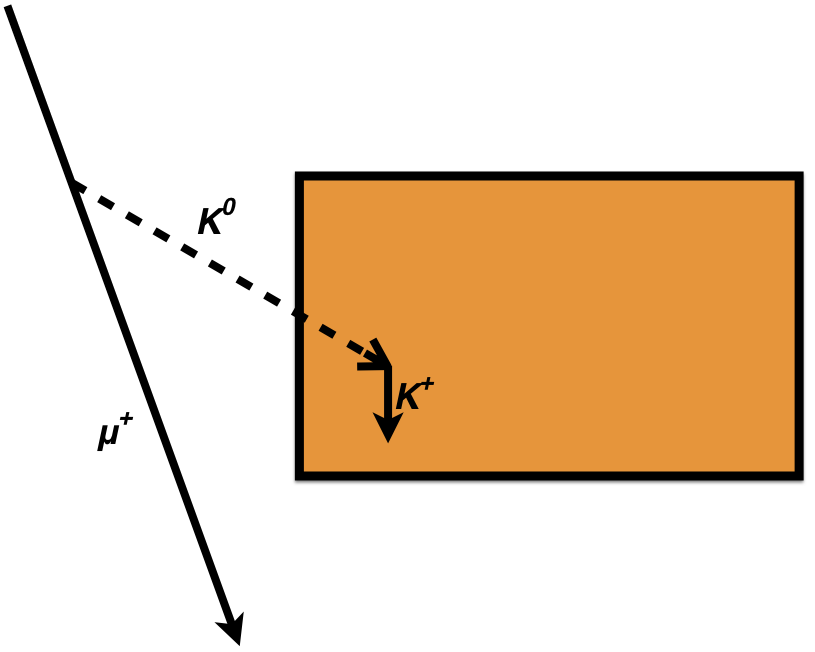
\includegraphics[width=0.5\textwidth]{KaonNDKInteraction}
  \caption[How the interaction of a cosmic muon can mimic a nucleon decay signature]
          {How the interaction of a cosmic muon can mimic a nucleon decay signature, by producing a $K^{0}_{L}$ which interacts far from the detector wall, producing an isolated kaon.}
  \label{fig:K0LongBackground}
\end{figure}


%*******************************************************************************
%*********************************** Chapter DUNE ******************************
%*******************************************************************************
\chapter{The Deep Underground Neutrino Experiment}  %Title of chapter

\graphicspath{{DUNE/Figs/PDF/}{DUNE/Figs/Raster/}{DUNE/Figs/Vector}}

\nomenclature[a-tick]{tick}{Unit of time equal to 500 ns}
\nomenclature[z-CRC]{CRC}{Cosmic Ray Counter}
\nomenclature[z-SiPM]{ADC}{Analogue to Digital Converter}
\nomenclature[z-TPC]{TPC}{Time Projection Chamber}
\nomenclature[z-SiPM]{SiPM}{Silicon Photo Multiplier}
\nomenclature[z-FD]{FD}{Far Detector}

%********************************** %First Section  **************************************
\section{DUNE location and beam line} %Section - X.1 

%********************************** %Second Section  *************************************
\section{The DUNE detectors and schedule} \label{sec:DUNEDetector} %Section - X.2

%********************************** %Third Section  *************************************
\section{Physics opportunities of DUNE} %Section - X.3

%********************************** % 3.1 Section  *************************************
\subsection{Neutrino physics}  %Section - X.3.1

%********************************** % 3.2 Section  *************************************
\subsection{Nucleon decay and supernovae neutrinos}  \label{sec:NDK_Atmos}%Section - X.3.2

\begin{table}[h!]
\caption[Nucleon decay limits in DUNE and Super-Kamiokande]
        {Nucleon decay limits in DUNE and Super-Kamiokande, in some favoured decay channels.}
\centering
\label{tab:NDKLim}
\begin{tabular}{c c c c}
\toprule
{Total flux (cm$^{-2}$ s$^{-1}$)} & {Mean E$_{\mu}$ (GeV)} & {Mean slant depth (m w.e)} & {Mean $\theta$ ($^{\circ}$)} \\ 
\midrule
5.66 $\times$ 10$^{-9}$           & 283                    & 4532                       & 26                           \\
\bottomrule
\end{tabular}
\end{table}

%********************************** % 3.3 Section  *************************************
\subsection{Background to nucleon decay} \label{sec:BkNDK}  %Section - X.3.3

\begin{figure}[h!]
  \centering
  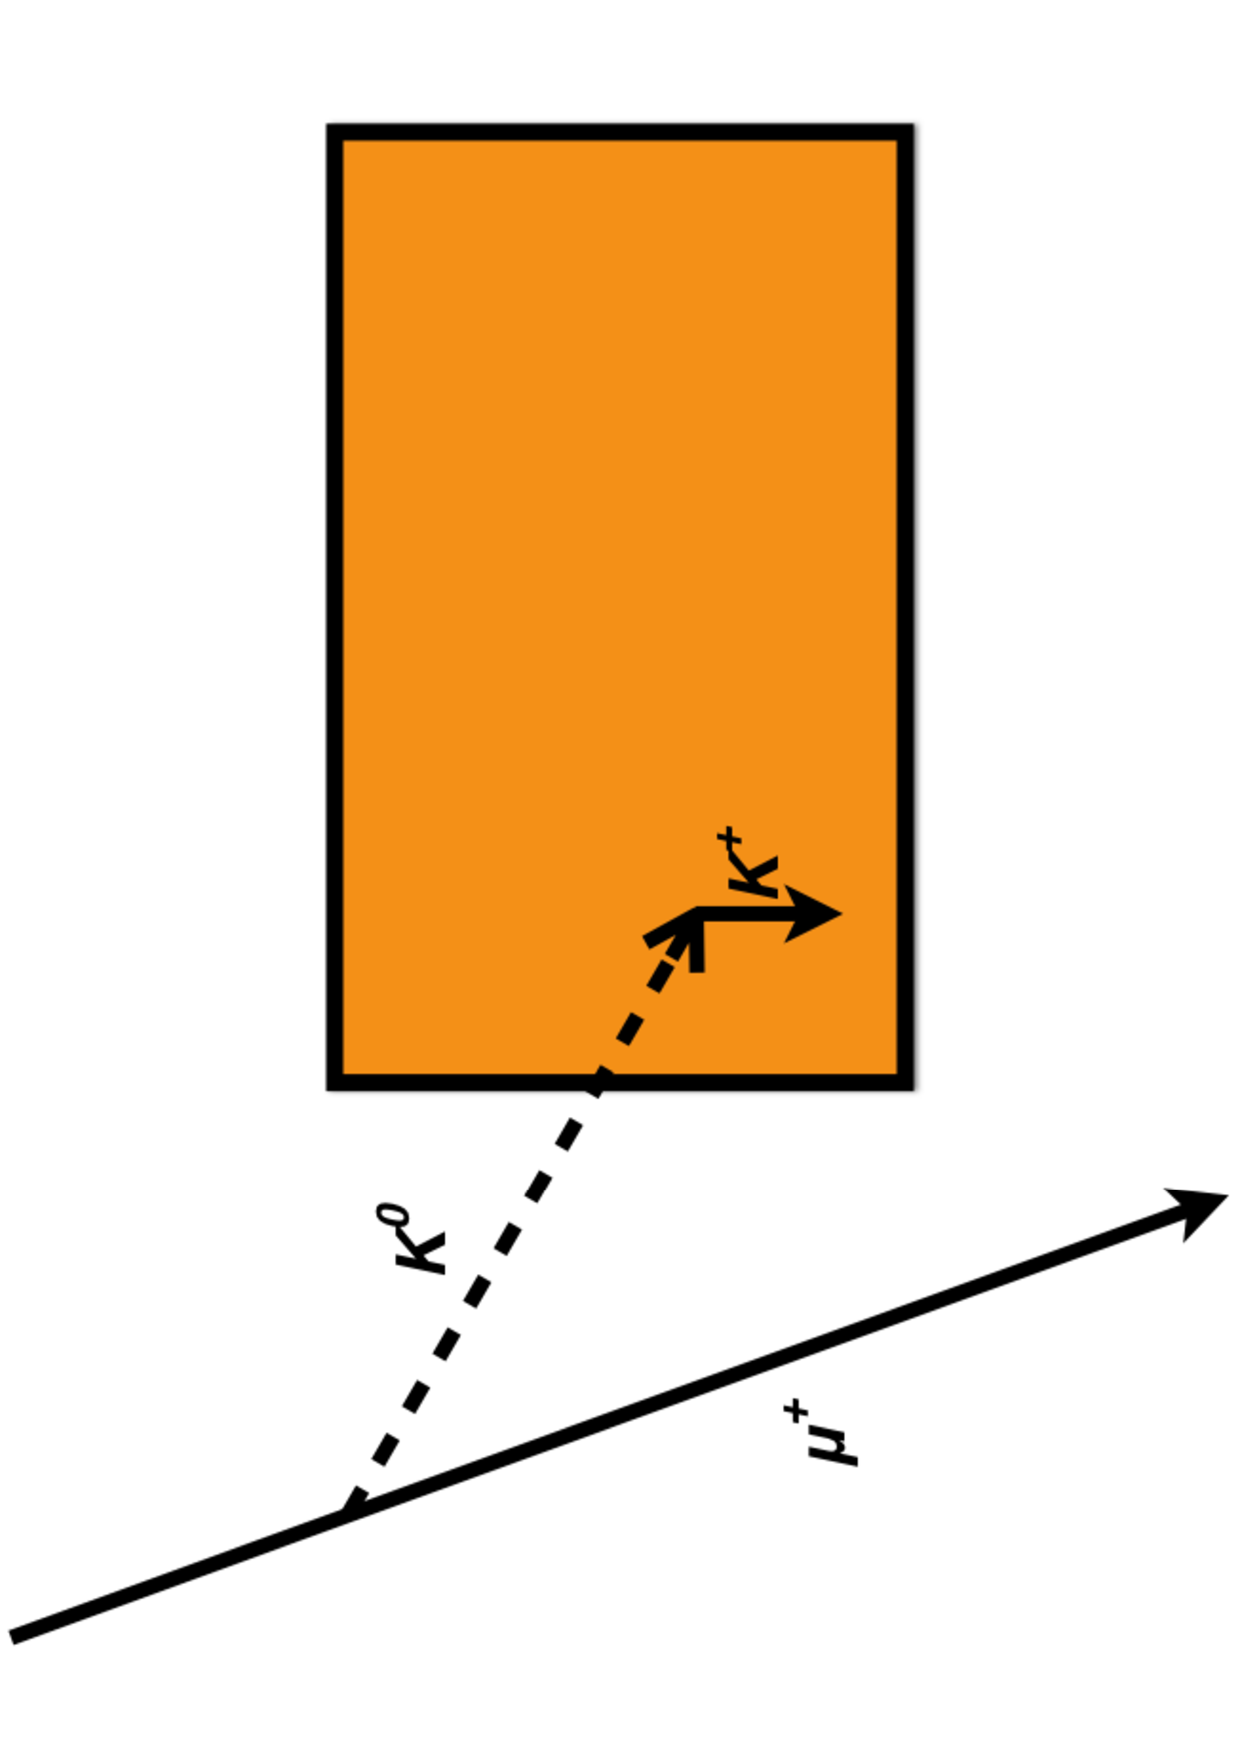
\includegraphics[width=0.5\textwidth]{KaonNDKInteraction}
  \caption[How the interaction of a cosmic muon can mimic a nucleon decay signature]
          {How the interaction of a cosmic muon can mimic a nucleon decay signature, by producing a $K^{0}_{L}$ which interacts far from the detector wall, producing an isolated kaon.}
  \label{fig:K0LongBackground}
\end{figure}

%********************************** % Fourth Section  *************************************
\section{Path to building DUNE - The 35 ton prototype} \label{sec:The35tonDetector}  %Section - X.4

\begin{figure}[h!]
  \centering
  %\includegraphics[width=0.85\textwidth]{}
  \caption[The wrapped wires of the 35 ton]{A schematic showing what the wrapped wire planes of the DUNE detector designs looked like in the 35 ton.}
  \label{fig:35tonWireGeom}
\end{figure}

\begin{figure}[h!]
  \centering
  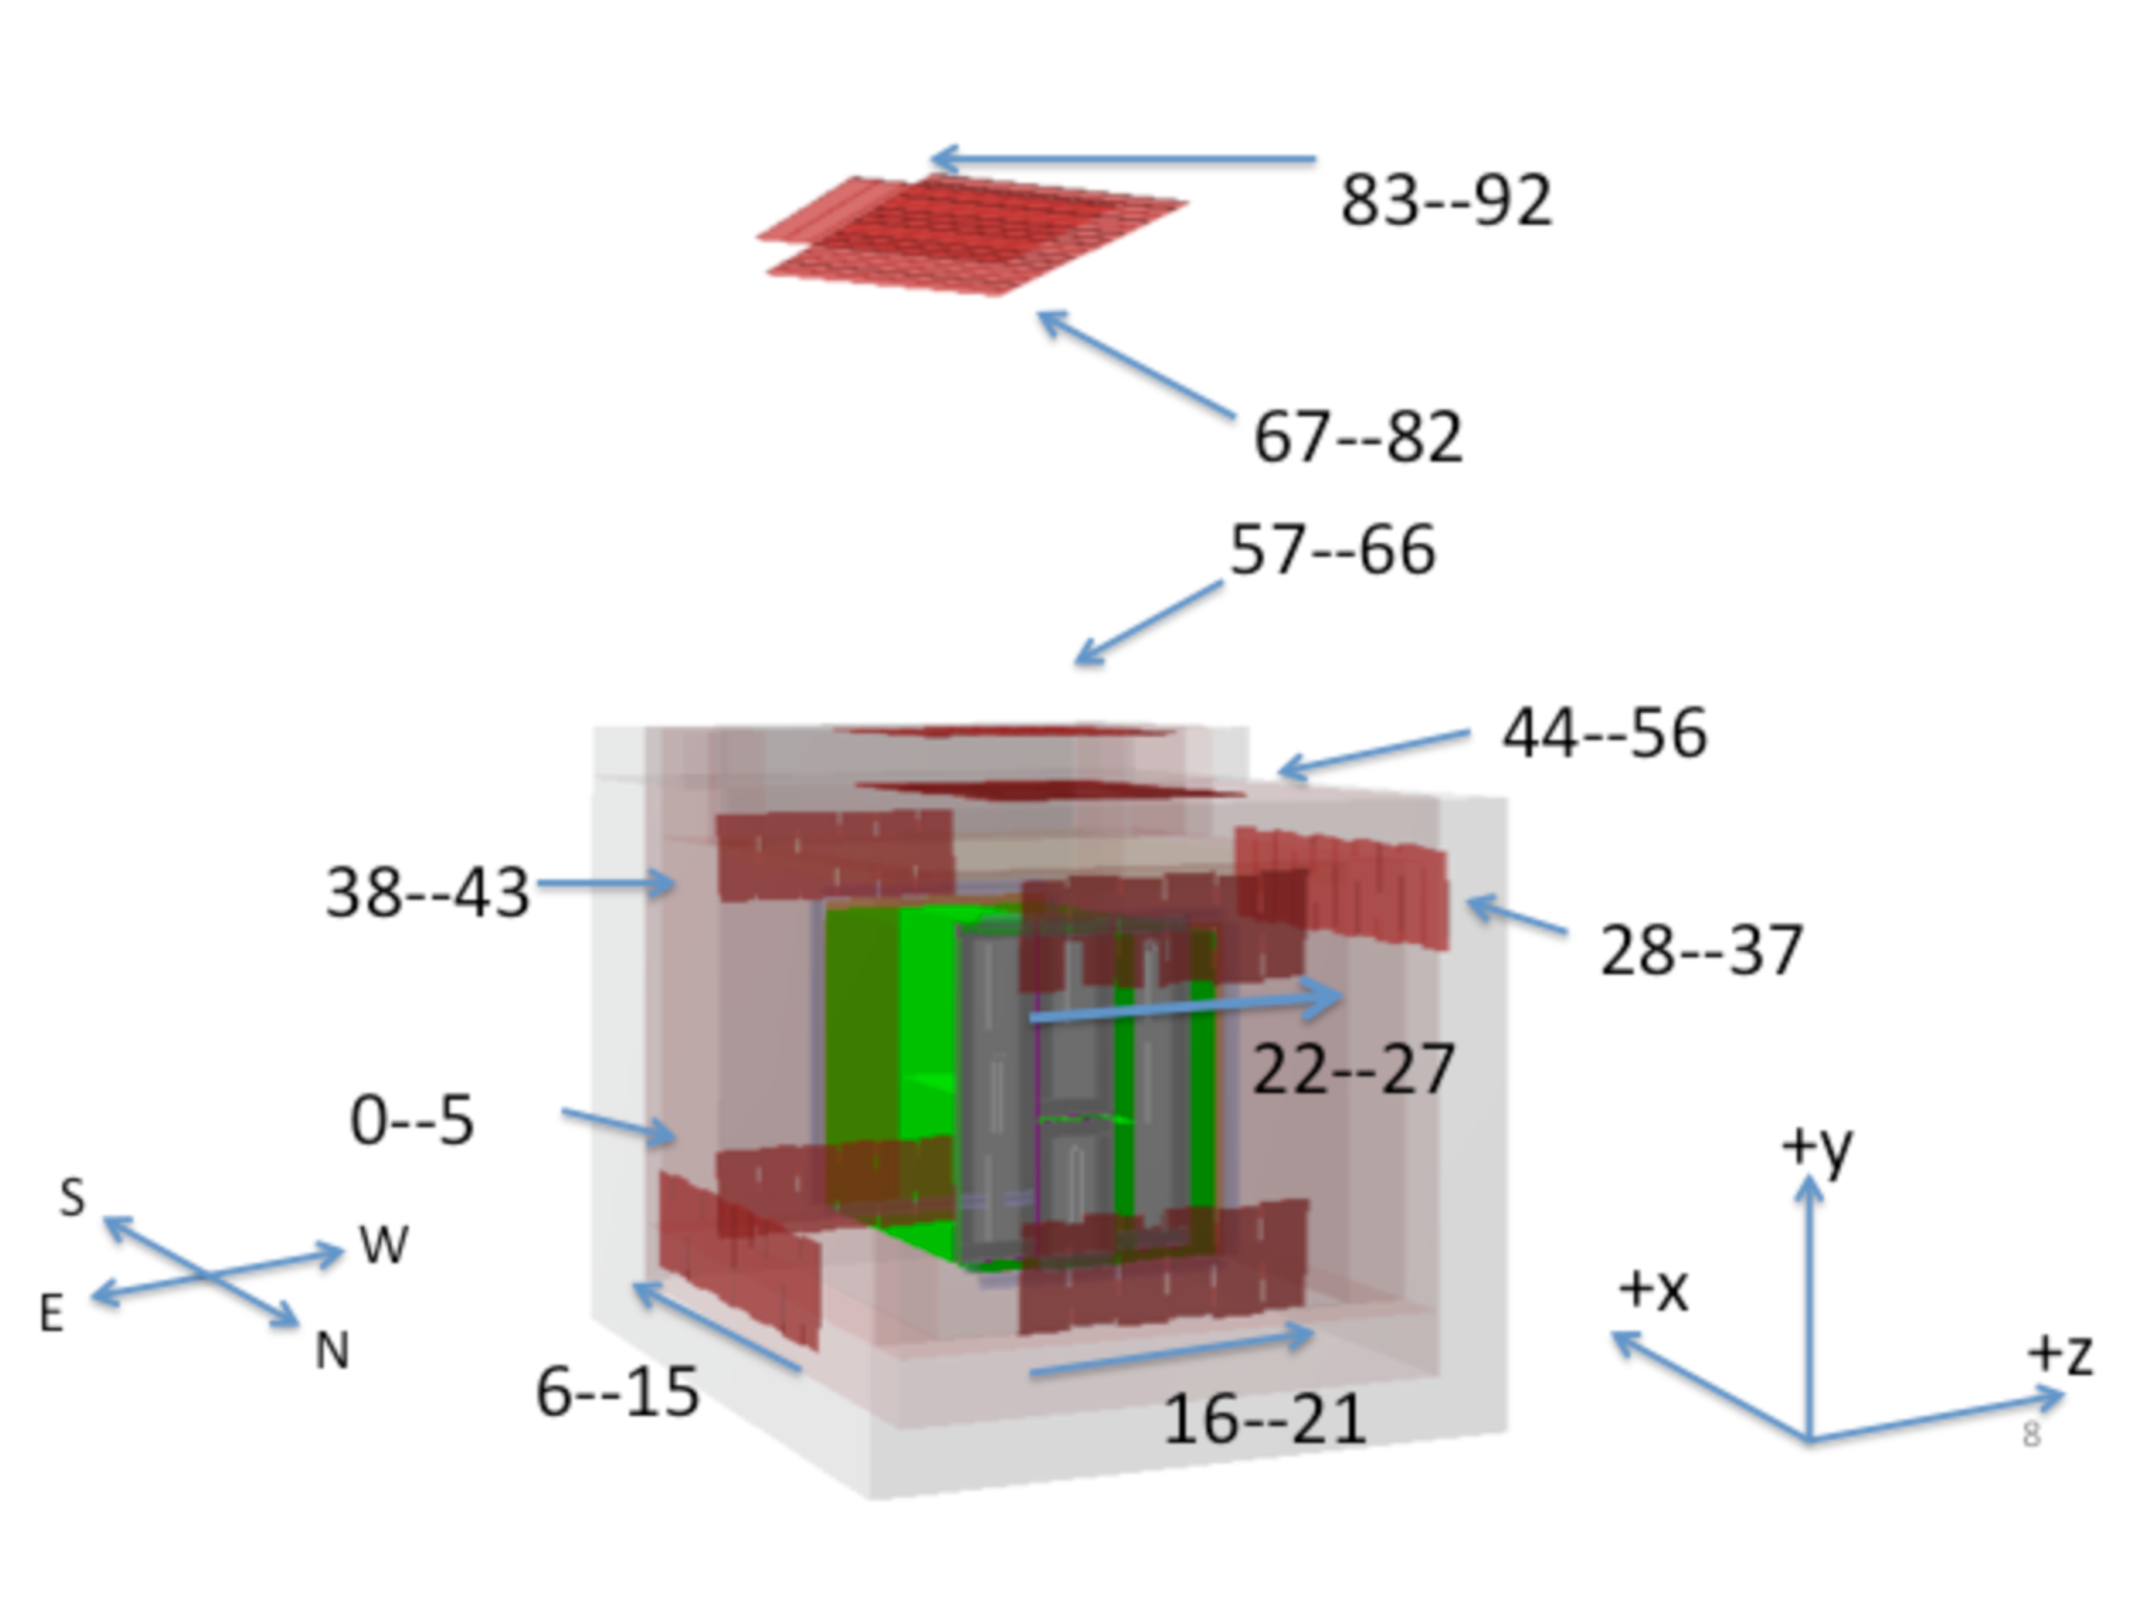
\includegraphics[width=0.85\textwidth]{35tonFullDetect}
  \caption[A representation of the counter locations in the 35 ton]
          {A representation of the counter locations in the 35 ton, with the magnetic and LArSoft co-ordinate systems shown. The other detector components can be seen inside the cryostat, such that the counters on the North wall are behind the short drift volume. The East - West counters are numbered 6-15 and 28-37 respectively. The North Lower - South Upper counters are numbered 16-21 and 38 - 43 respectively. The North Upper - South Lower counters are numbered 22-27 and 0-5 respectively. The telescope triggers are numbered 44-92 and are split into four groups.}
  \label{fig:35tonCounterLoc}
\end{figure}

%********************************** % Fifth Section  *************************************
\section{The DUNE software} \label{sec:LArSoft} %Section - X.5
The software package used by DUNE is called LArSoft~\citep{Church_LArSoft}~\citep{LArSoftOrg} which is a simulation, reconstruction and analysis package for Liquid Argon Time Projection Chamber (LArTPC) that is being used by many experiments in the US neutrino program. LArSoft has been developed to be detector agnostic, meaning that much of the code is shared between experiments. To this end it is envisioned that it will be used as a platform for constant development in existing experiments and those still in the planning phases such as DUNE. LArSoft is built around the Fermilab-supported \emph{analysis reconstruction framework} (\emph{art}). External packages such as ROOT~\citep{ROOT} and GEANT4~\citep{GEANT4} are incorporated into LArSoft meaning that the user does not have to coordinate specific versions of the packages as the newest versions are automatically incorporated. \\

There are numerous mechanisms by which particles can be generated within the software with external packages. One such package is GENIE~\citep{GENIE} which is used to study neutrino interactions and nucleon decays. Another package, Nuance~\citep{Nuance}, is a neutrino interaction generator specifically for Liquid Argon (LAr). Finally, CRY~\citep{CRY} and CORSIKA!!!citep{CORSIKA} are cosmic ray events generators which are used to simulate the expected event rates for surface detector locations in absence of a neutrino beam. Recently the MUon Simulations UNderground (MUSUN)~\citep{MUSUN}~\citep{MUSUN2} generator which takes the output of MUon SImulation Code (MUSIC)~\citep{MUSUN}~\citep{MUSIC}~\citep{MUSIC2} has also been incorporated, see Section~\ref{sec:FDIncorporation} for further details. It is also possible to use an inbuilt single particle generation mode which is fully tuneable as particle type, momenta, positions and directions can all be varied. \\

The co-ordinates and angles in LArSoft are defined as follows, and schematic representations of how this appears in the 35 ton are shown in Figure~\ref{fig:LArSoft_coords}:
\begin{itemize}
\item $x$ - The beam direction, with maximal $x$ being where the beam enters the detector.
  \begin{itemize}
  \item In the 35 ton prototype where there is no beam positive $x$ is in the opposite direction to that which electrons drift in the large TPC, where $x$ = 0 is the position of the APA frames in the long drift volume.
  \item In the far detector geometry $x$ = 0 is defined as the midpoint between the two rows of CPAs 
  \end{itemize}
\item $y$ - The vertical direction, with maximal $y$ being the most highest point.
  \begin{itemize}
  \item In the 35 ton $y$ = 0 is halfway between the gap created by the two centre APAs which are mounted one above the other.
  \item In the far detector $y$ = 0 is defined as the midpoint between the two vertical layers of TPCs.
  \end {itemize}
\item $z$ - Defined as such to have a right handed co-ordinate system.
  \begin{itemize}
  \item In the 35 ton $z$ = 0 is at the edge of the leftmost APA frame when looking down the long drift volume.
  \item In the far detector $z$ = 0 is defined at the edge of the leftmost APA frame when looking down the long drift volume.
  \end{itemize}
\item $\theta$ - The angle that a vector makes from the $x$ axis in the $xy$ plane.
\item $\phi$ - The angle between the $z$ axis and the vector.
\end{itemize}

\begin{figure}[h!]
  \centering
  \begin{subfigure}{0.45\textwidth}
    \centering
    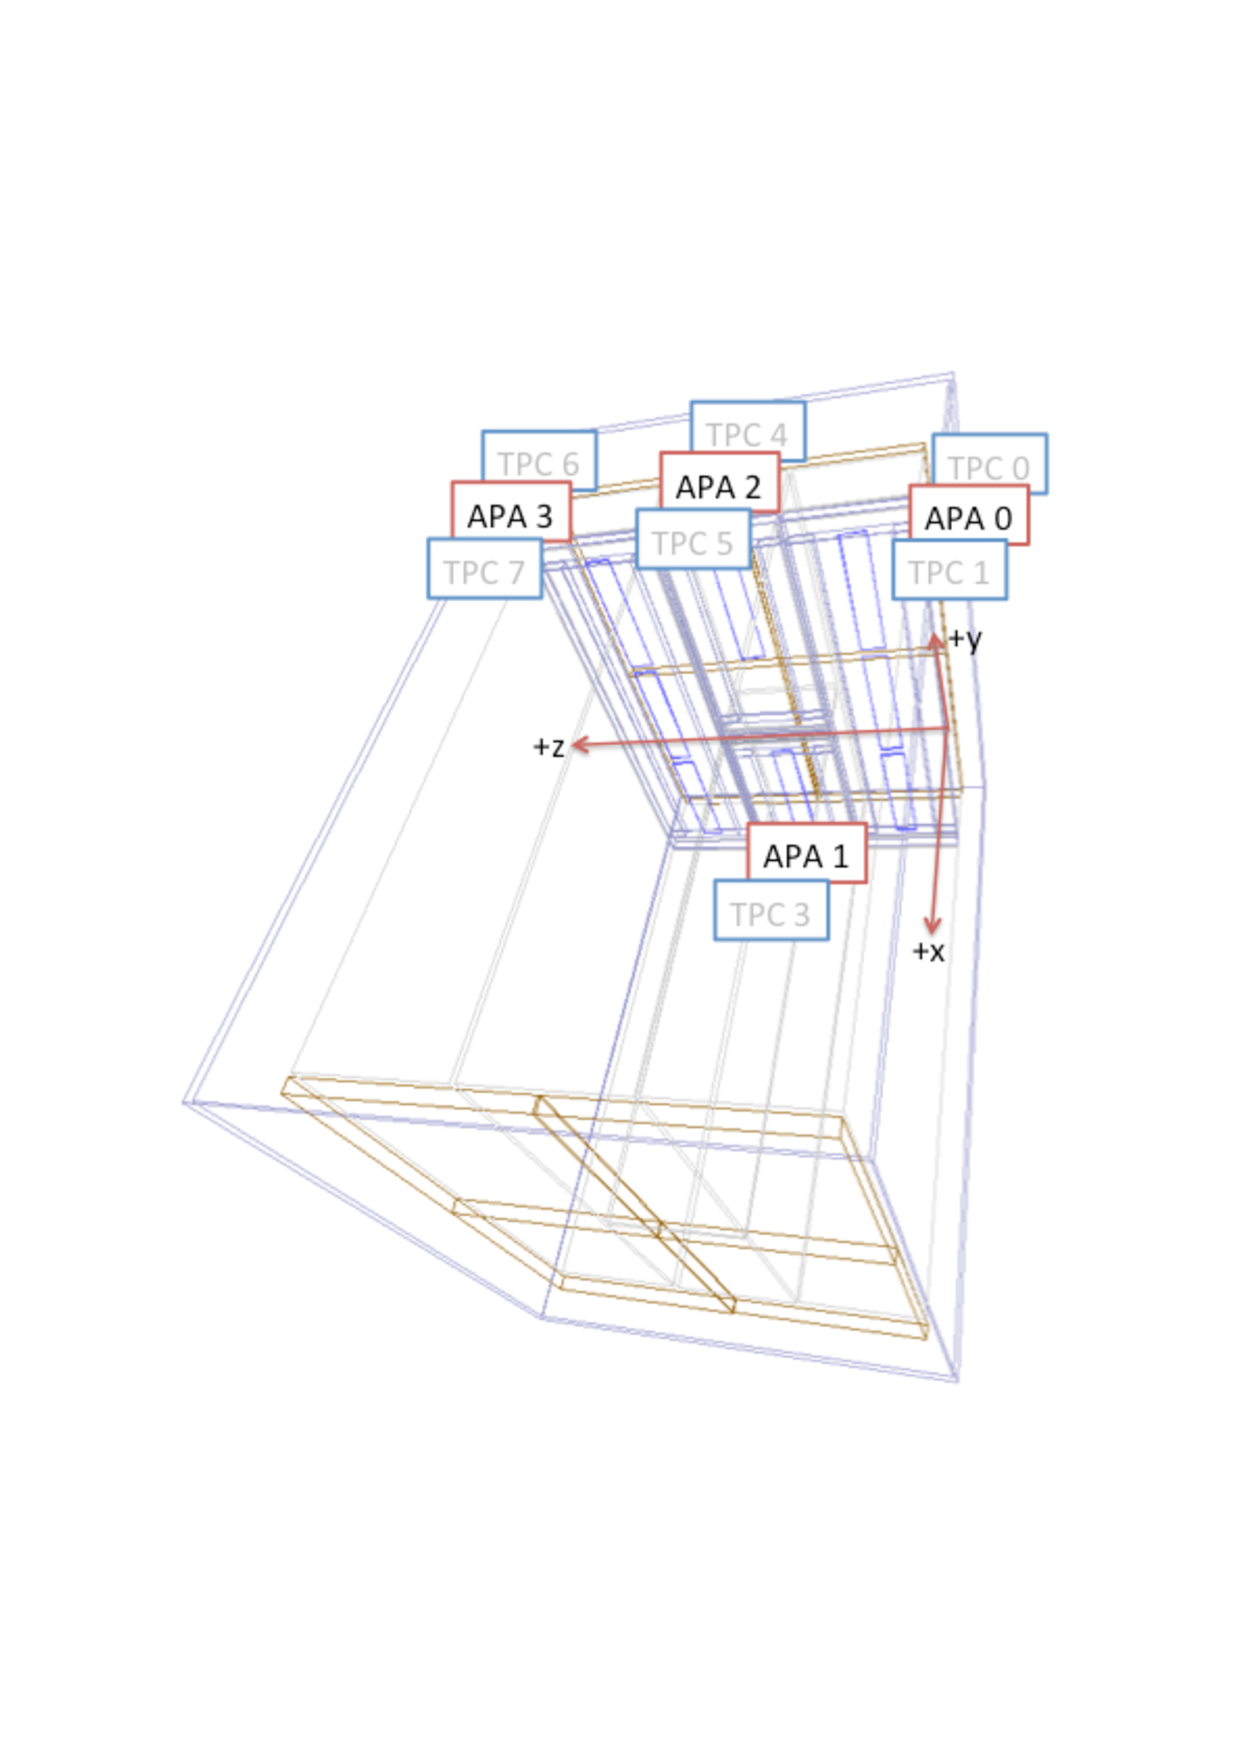
\includegraphics[width=\textwidth]{35ton_APASchem}
    \caption{The location of the origin of the 35 ton co-ordinate system in 3D.}
  \end{subfigure}
  \hspace{0.08\textwidth}
  \begin{subfigure}{0.45\textwidth}
    \centering
    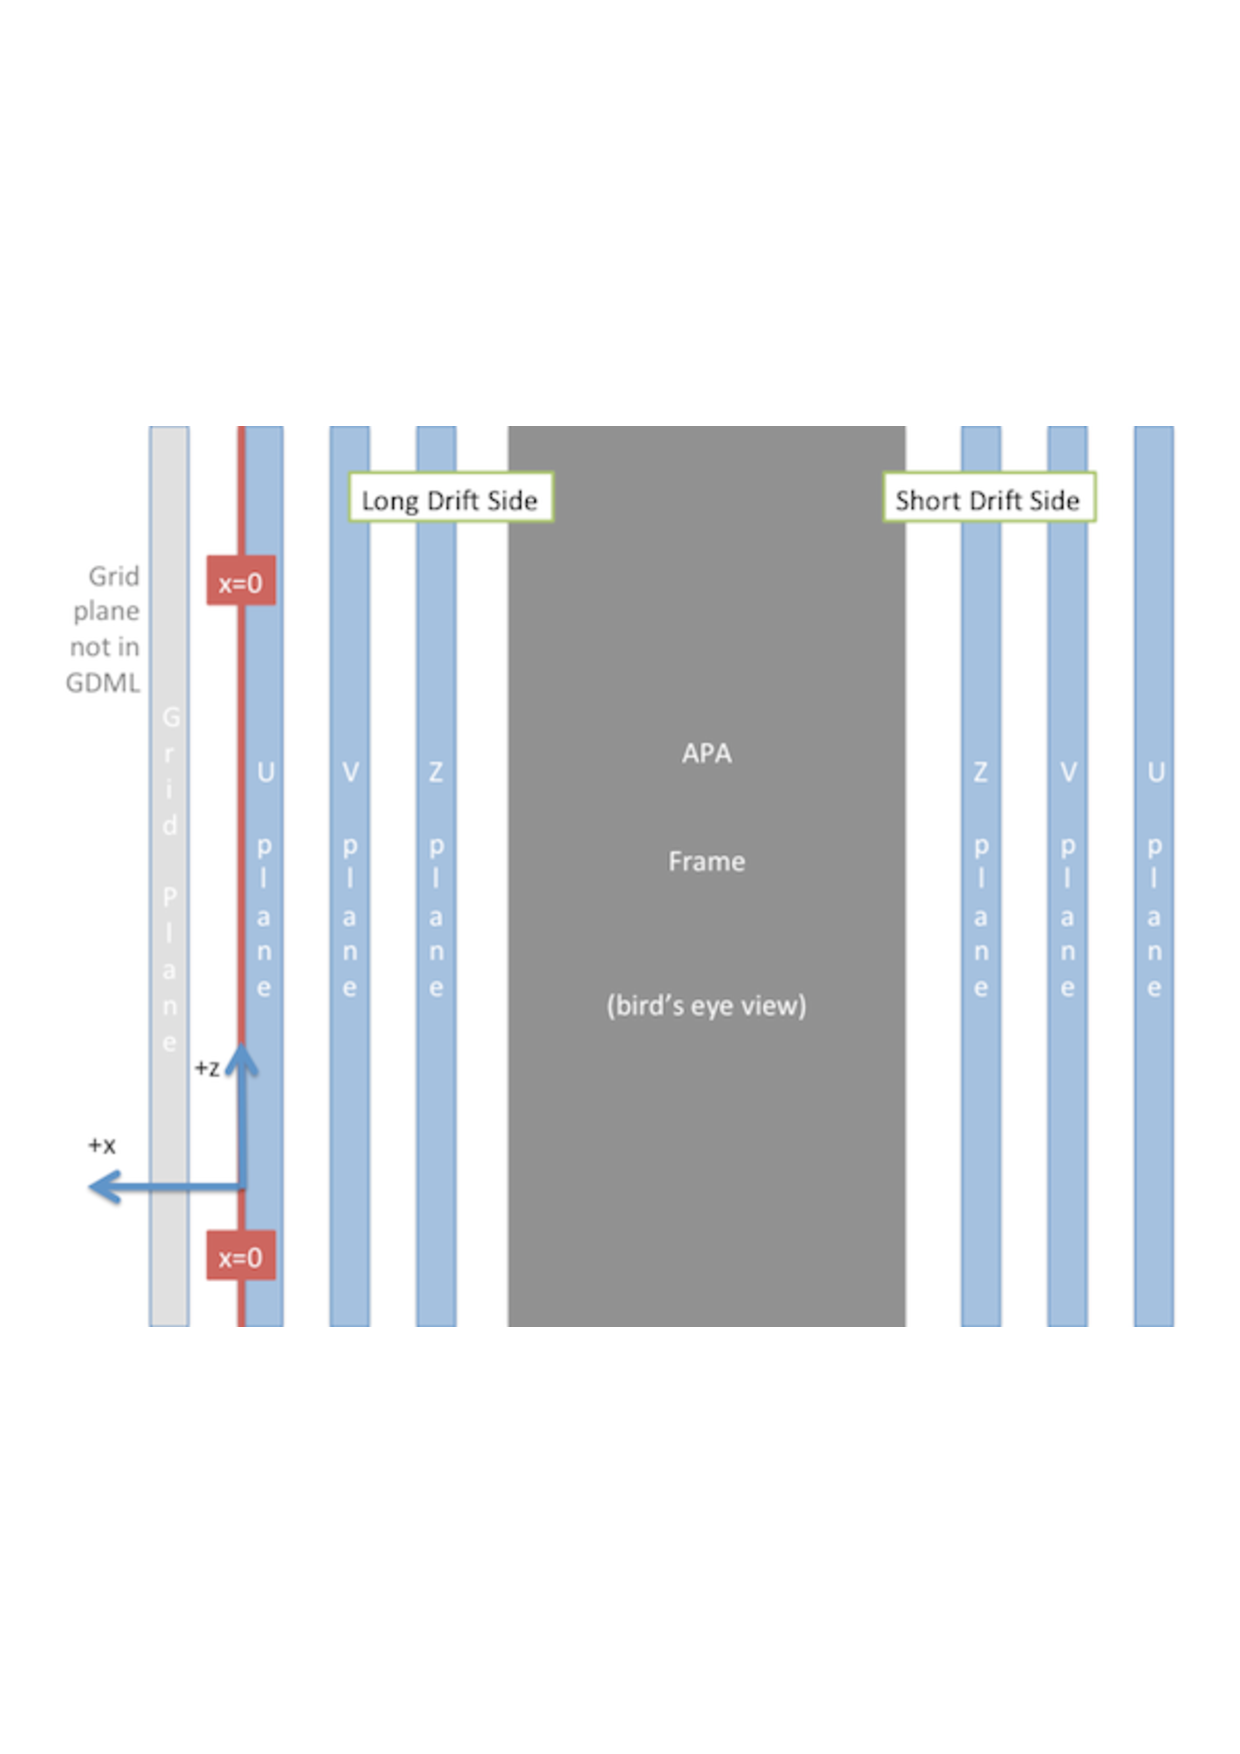
\includegraphics[width=\textwidth]{35ton_xCenter}
    \caption{The location of the origin of the 35 ton co-ordinate system in a 2D aerial view.}
  \end{subfigure}
  \caption[The LArSoft co-ordinate system as it is represented in the 35 ton.]
          {The LArSoft co-ordinate system as it is represented in the 35 ton. Left shows the location of the origin relative to the TPC detector components. The four APAs, and eight TPCs are shown, where the even numbered TPCs are on the short drift side, $\sim$20 cm drift, and the odd numbered TPCs are on the long drift side, $\sim$250 cm drift. The CPAs are also shown as the objects with a brown outline. Right shows the location of the origin with respect to the APAs. The wire planes are shown, the U and V planes are induction wires, whilst the Z planes are collection wires.}
  \label{fig:LArSoft_coords}
\end{figure}

The simulation of particles is usually split into five separate distinct processes to reflect the different stages in which development often progresses. The advantage of segmenting the computational process in this way is that improvements can easily applied to a file without rerunning the entire chain. This is especially important when large Monte Carlo or data samples are produced for general use within collaborations so that users are able to concentrate on improving a specific part of the computational process. When these all-purpose samples are produced the analysis performed provides users with any Monte Carlo truth information along with the reconstructed quantities for use in analyses performed outside LArSoft. The computational process is often broken down in the following way:
\begin{itemize}
\item Particle generator.
\item Particle transport using GEANT4.
\item Full detector simulation, including detector responses. 
\item Full event reconstruction.
\item Analysis.
\end{itemize}

Later significant focus will be given to the reconstruction of TPC data, and so it is necessary to briefly illustrate the mechanisms by which TPC data is reconstructed in LArSoft. Much of the information presented below is summarised in~\citep{LArSoftRecoNote}~\citep{LArSoftOrg}. After the full detector simulation or data taking, detector effects such as the electronics response function and a pedestal offset have to removed. Once these effects are removed the signal is estimated using the optimal value of $signal/noise$ which would produce the measured signal. This process, called deconvolution, does not conserve pulse height and is not guaranteed to preserve the normalisation. The deconvoluted signals are all unipolar distributions which means that Gaussian distributions can then be fitted to them when trying to reconstruct hits. This is shown in Figure~\ref{fig:LotsOfHits}, and explained further below.\\

\begin{figure}[h!]
  \centering
  \begin{subfigure}{0.95\textwidth}
    \centering
    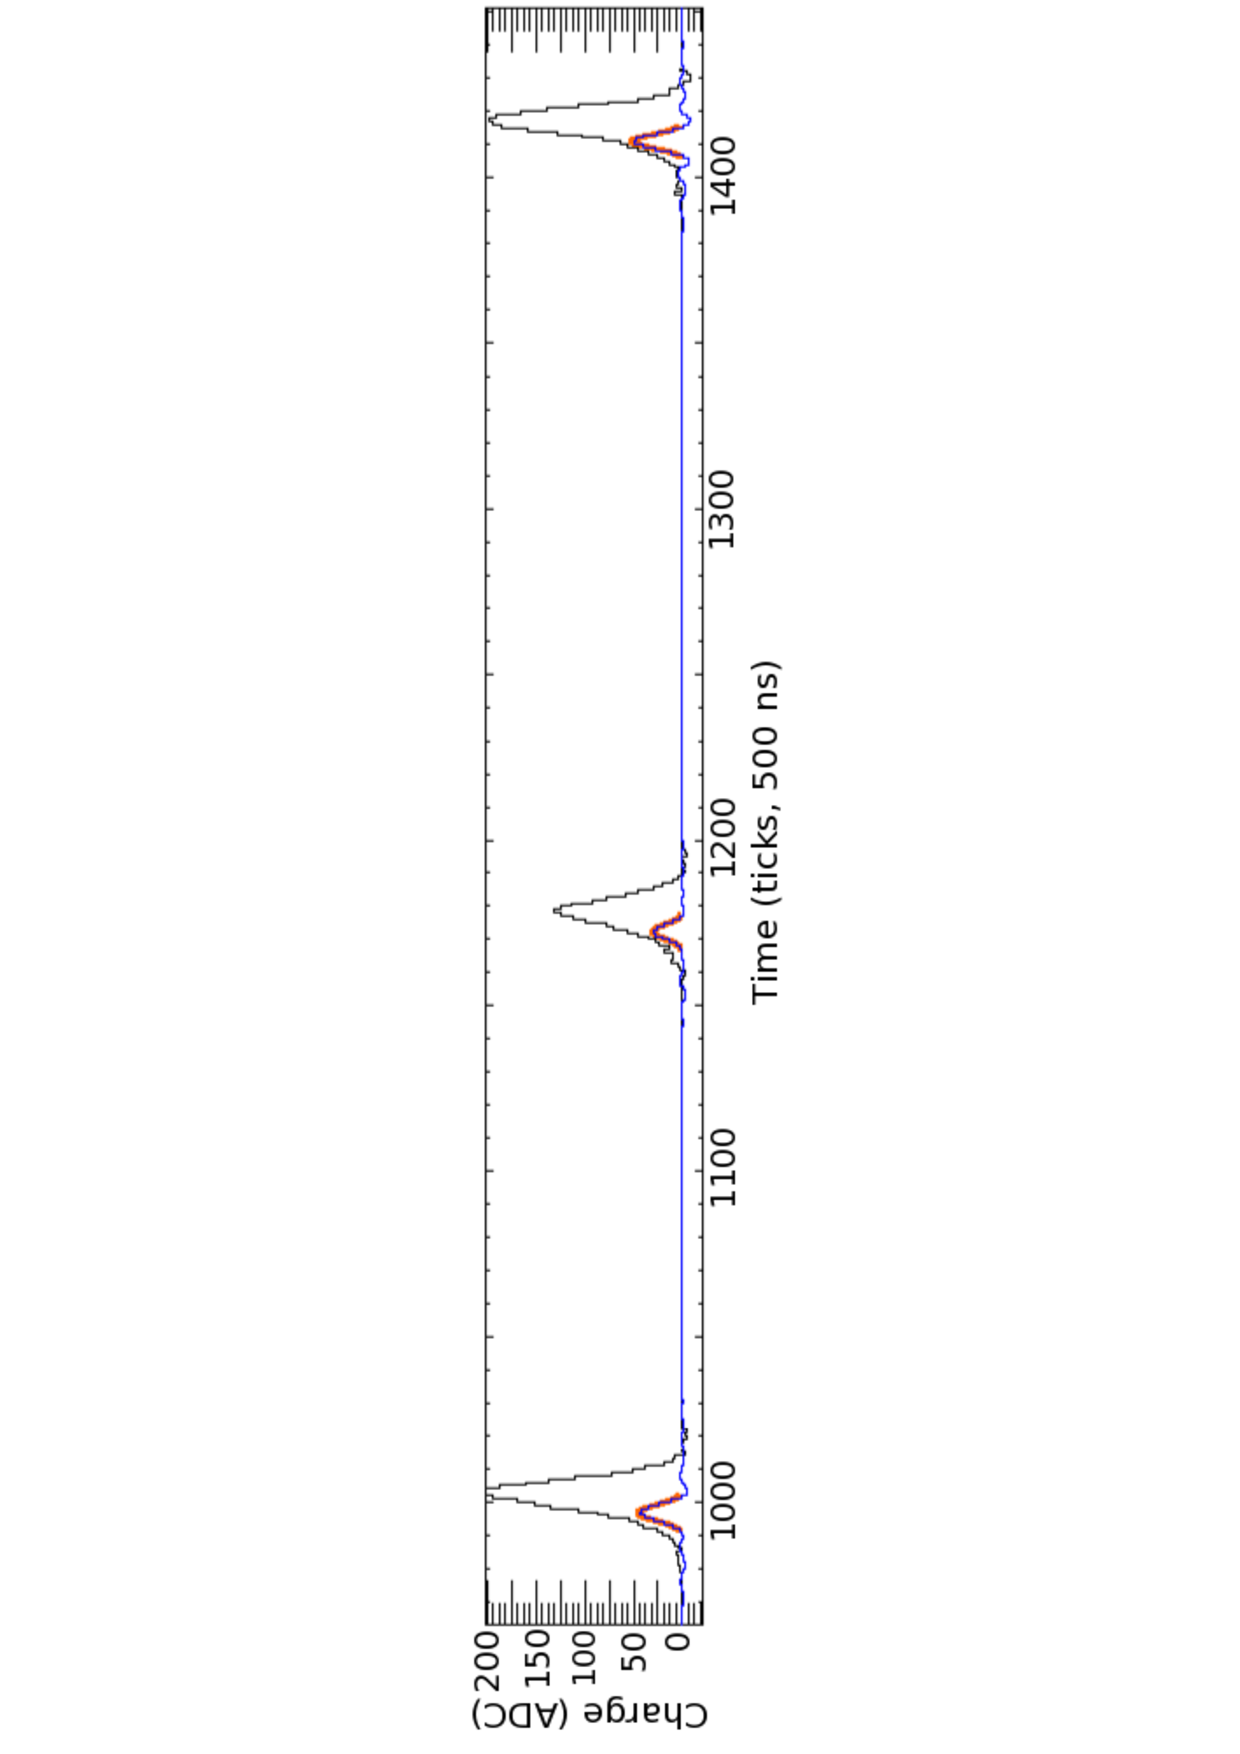
\includegraphics[width=\textwidth]{CollectionPlane}
    \caption{Collection plane depositions.}
    \label{fig:LotsOfHits_Col}
  \end{subfigure}
  \begin{subfigure}{0.95\textwidth}
    \centering
    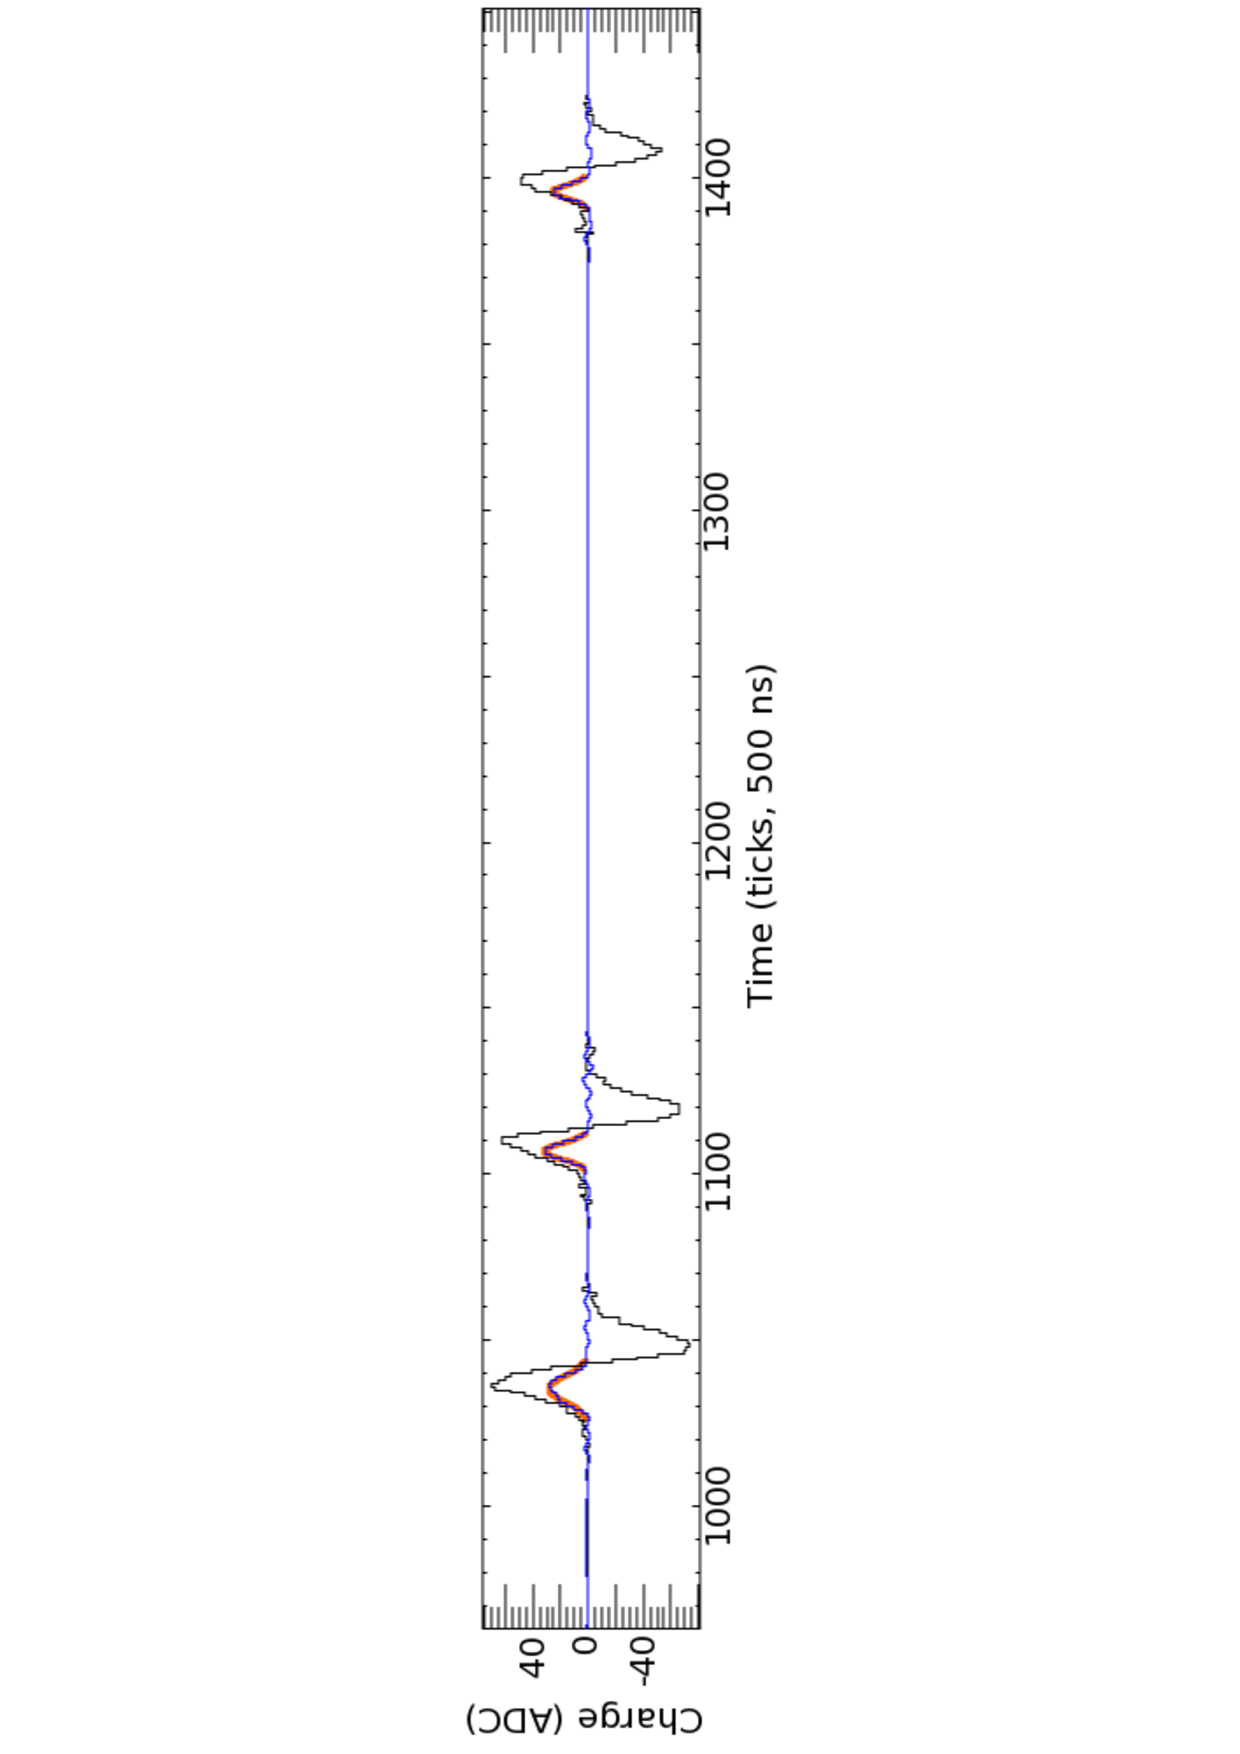
\includegraphics[width=\textwidth]{InductionPlane}
    \caption{Induction plane depositions.}
    \label{fig:LotsOfHits_Ind}
  \end{subfigure}
  \begin{subfigure}{0.95\textwidth}
    \centering
    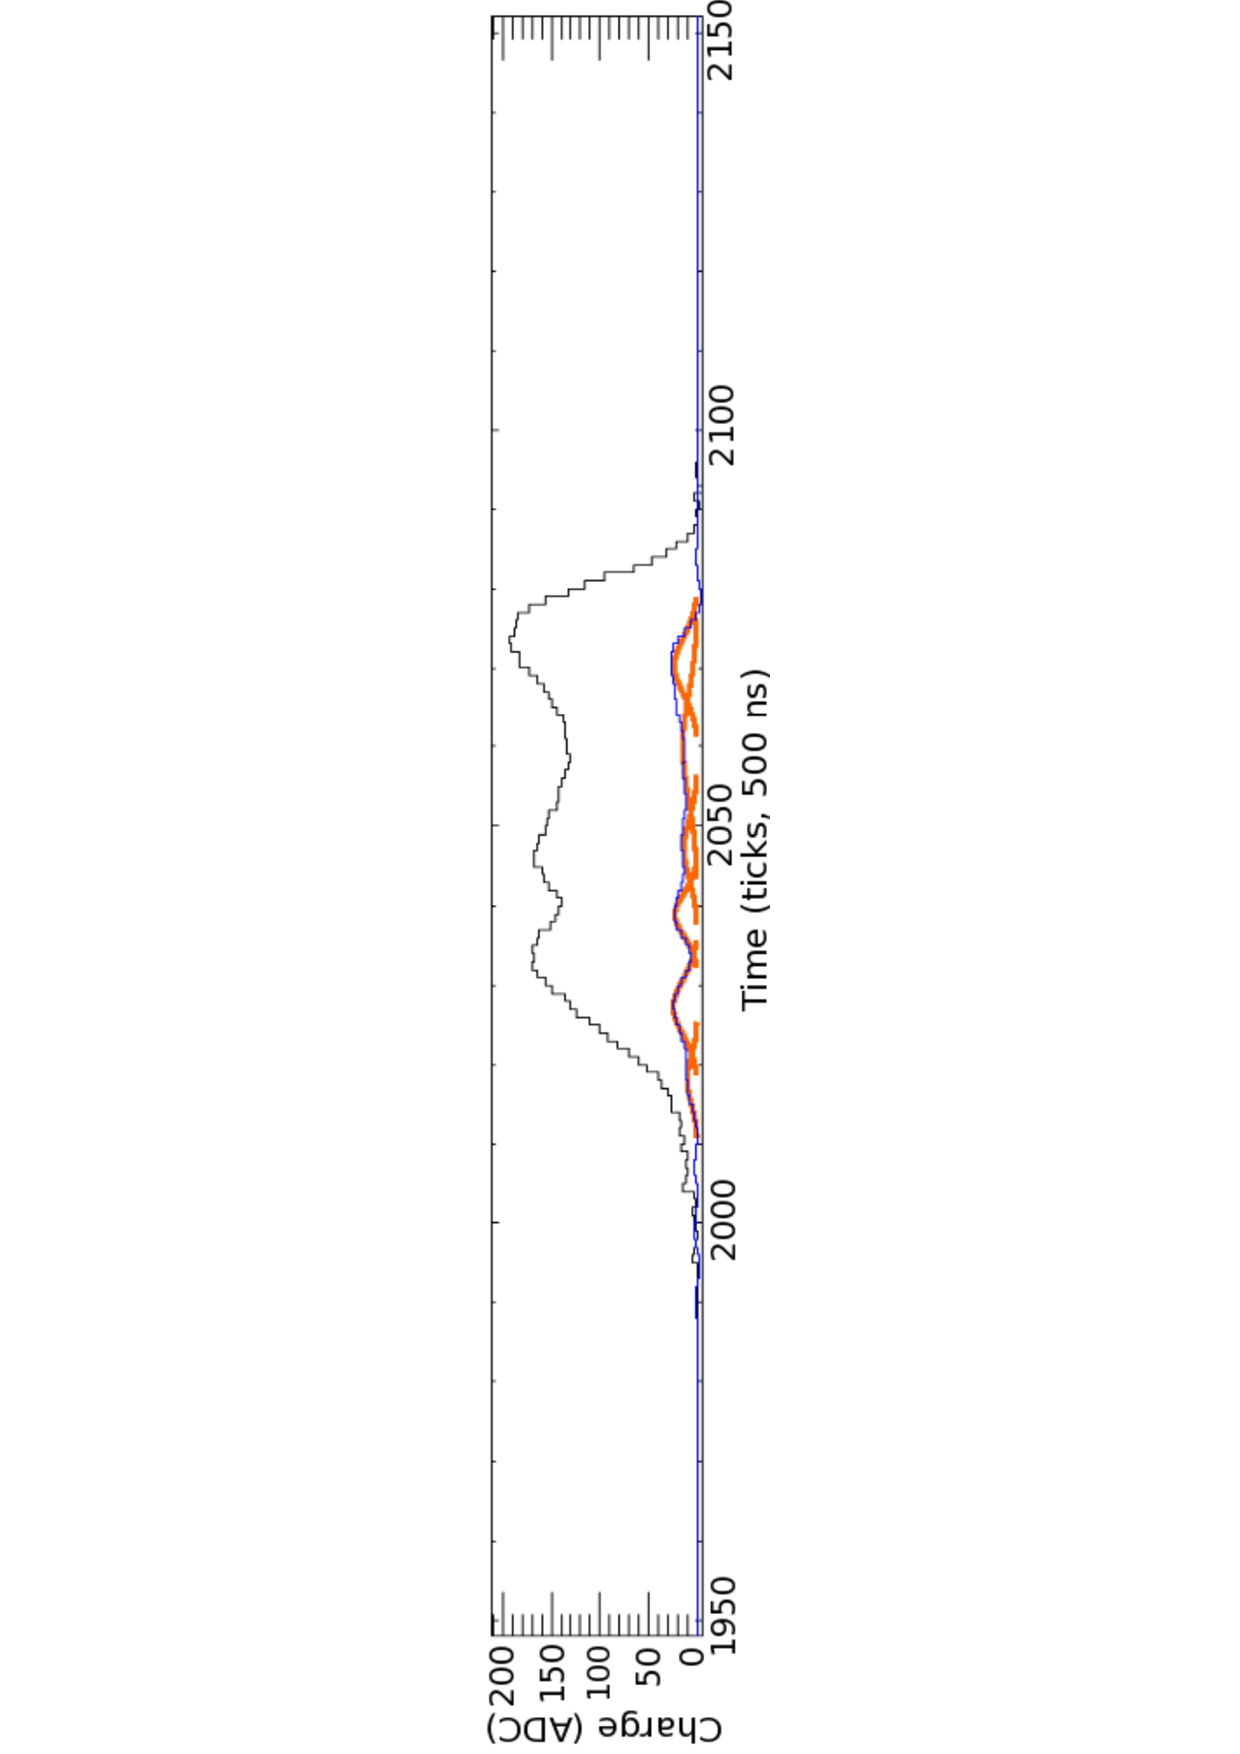
\includegraphics[width=\textwidth]{Complex}
    \caption{A large collection plane deposition over a large period of time.}
    \label{fig:LotsOfHits_Big}
  \end{subfigure}
  \caption[Reconstructed hits from simulated energy depositions]
          {The raw and deconvoluted signals with reconstructed hits on single wires for simulated energy depositions. The depositions, from particles generated by CRY, are not from a single event and have been selected for demonstration purposes only. The plots are shown with increasing charge (ADC) on the $y$ axis, and increasing time (ticks, 500 ns) on the $x$ axis. The black lines represent the raw signals, the blue lines represent the deconvoluted signals and the orange lines represent the reconstructed hits. Top shows depositions on a collection plane wire, it can be seen that the raw signal is unipolar. Middle shows depositions on an induction plane wire, it can be seen that the raw signal is bi-polar whilst the deconvoluted signal and reconstructed hits are unipolar. Bottom shows a complex deposition on a collection plane wire, where multiple reconstructed hits are required to reproduce the deconvoluted signal.}
  \label{fig:LotsOfHits}
\end{figure}

The deconvoluted signals are reconstructed into hits by identifying regions that are above a threshold value and then attempting to replicate the signal in these regions by introducing Gaussian distributions. For isolated hits this is typically achieved using only one Gaussian distribution, however for large energy depositions over a large period time where many particles are involved, multiple Gaussian distributions are often required. Large energy depositions are also possible when the direction of the particle aligns with a wire, this means that all of the deposited energy is collected on this single wire. Examples of reconstructed hits are shown in Figure~\ref{fig:LotsOfHits}. These figures are taken from separate CRY simulated events, and so do not correspond to a continuous simulated event. They have been selected only as a demonstration of the process of hit reconstruction. Figures~\ref{fig:LotsOfHits_Col} and~\ref{fig:LotsOfHits_Ind} show multiple time-separated energy depositions on a collection and induction wire respectively. A more complex energy deposition on a collection plane wire is shown in Figure~\ref{fig:LotsOfHits_Big} where energy depositions from many particles at similar times have created a complicated energy deposition that requires many reconstructed hits to explain. \\

As noted in Section~\ref{sec:DUNEDetector} and Section~\ref{sec:The35tonDetector} the DUNE FD and the 35 ton both have wrapped wires on the induction planes. A result of this is that the location of the reconstructed hit on an induction wire is ambiguous as a single wire has many wire segments, as shown in Figure~\ref{fig:35tonWireGeom}. An important feature of this ambiguity is that the TPC in which the hit occurred cannot be identified unless it is combined with another hit. These ambiguities do not extend to the collection plane wires as they are not wrapped and so consist of only a single wire segment in a single TPC. Hits are combined across the three planes by identifying wire segments on each plane which intersect and have hits at common times. In the traditional reconstruction process only hits that make these so-called 'triple points' are considered disambiguated, with other hits being identified as noise hits causing them to be discarded. \\

The inclination of the wire planes has to be carefully chosen so as to minimise both the number of wires required and the number of times that wire triplets intersect. This is shown in Figure~\ref{fig:WirePitches}, where the wire inclinations used in the 35 ton detector, are compared to those in the DUNE FD reference design. The inclination of wires in the 35 ton was 45$^{\circ}$ $\pm$ 0.7$^{\circ}$ meaning that many wire triplets cross twice and some wire pairs cross three times. When wire triplets cross multiple times the triplet which has the smallest distance between the common intersection point and the two, two-wire intersection points, is chosen as the best intersection candidate. This is shown as the 'Good intersection' on the right panel in Figure~\ref{fig:WirePitches}. The different wire pitches are necessary so that one of the triple points can be evaluated to be a better candidate, as with a wire pitch of 45$^{\circ}$ it can be impossible to distinguish between different triple points. The inclination of wires in the FD was chosen to be 36$^{\circ}$ to remove the possibility of multiple intersection points, as given the geometry of the APAs multiple intersection points are impossible and so disambiguation is much simpler. The lower inclination results in more induction wires being required though, making it more expensive to instrument the detector. It is also important that all wires on a given APA are either read at the top or base of the APA, depending on whether the APA is at either the top or the base of the detector respectively. This is because there must be minimal space between TPCs in the DUNE FD to reduce the internal dead space, and so TPCs cannot be read out along the sides as this would require a non-negligible amount of space to accommodate the cabling.\\

\begin{figure}[h!]
  \centering
  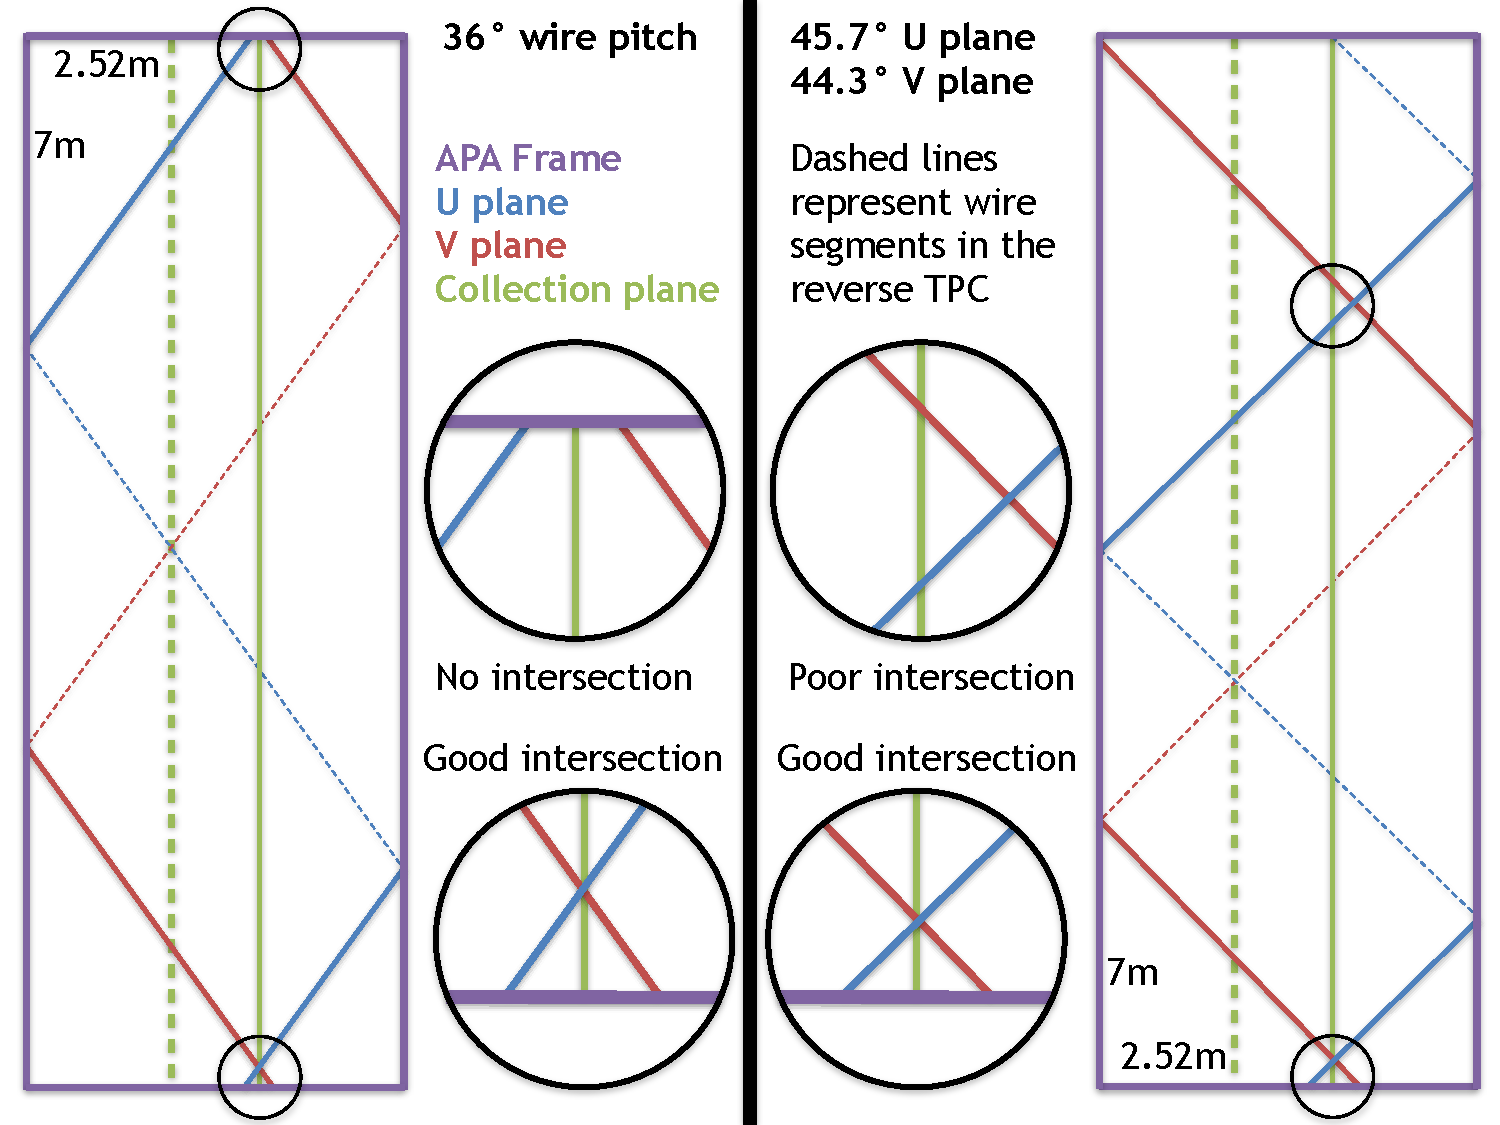
\includegraphics[width=0.85\textwidth]{WireAngleCondition}
  \caption[Performing disambiguation with different wire pitches.]
          {The effect that different wire pitches have on the ability to perform disambiguation in APAs with the far detector geometry. The left panel shows a wire pitch of 36$^{\circ}$, which is the reference design for the far detector, whilst the right panel shows wire pitches of 45$^{\circ}$ $\pm$ 0.7$^{\circ}$, as was used in the 35 ton. The left panel shows that only one 'triple point' can be made with the three wires shown, and so disambiguation is relatively trivial. The right panel shows that two 'triple points' can be made with the three wires shown, the 'triple point' where the three wires have a common intersection point is labelled as a 'good intersection' and it is this intersection point which would be chosen for the disambiguated hit.}
  \label{fig:WirePitches}
\end{figure}

Once the hits have been disambiguated they are combined to make clusters in each of the three planes, before the clusters are merged to make reconstructed tracks or showers. The clustering process is usually performed in wire-tick space on each plane separately, where all the hits from a single track or shower should be make a single cluster on each plane. It is possible to seed the start of clusters by using imaging techniques such as a Harris transform~\citep{HarrisTrans}, or to identify straight lines by using Hough transforms~\citep{HoughTrans}. As hits from a physical entity are unlikely to remain on a single channel or all come at identical times, clusters are often spread out over many channels for a range of times especially when performing clustering for showers. \\

Once clusters have been identified in each plane they can then be merged into 3-dimensional tracks and showers. The two most common tracking algorithms are PMTrack~\citep{PMTrack} and Pandora~\citep{Pandora}, and the most common showering algorithm is EMShower~\citep{EMShower}. Once 3D objects have been reconstructed, the calorimetric quantities need to be determined, this is often done separately for each plane. Two models exist for calculating $\frac{dE}{dx}$ in LArSoft, Birks model~\citep{BirksModel} and a modified Box model~\citep{PIDA_Paper} which uses a correction to the Box model~\citep{BoxModel} at low values of $\frac{dE}{dx}$. Normally the modified Box model is used as it holds for both large and small ionisation's, whereas Birks model experiences difficulties at large ionisation's and the traditional Box model struggles at low $\frac{dE}{dx}$. Both models incorporated in LArSoft, calculate the $\frac{dE}{dx}$ of a hit using the deposited charge ($dQ$) and the track pitch ($dx$) of the hit as well as the conversion of ADC value to number of electrons ($C_{GeV \rightarrow e^{-}}$), a correction due to electron lifetime ($C_{lifetime}$), the LAr density ($\rho$), the electric field ($E_{field}$) and the tuneable electron recombination factors ($Recomb_{X}$). The series of equations used in Birks model are shown in Equation~\ref{eq:Birks}, whilst those used in the modified Box model are shown in Equation~\ref{eq:ModBox}. \\

\begin{subequations}
  \label{eq:Birks}
  \begin{align}
    \frac{dE}{dx} &= \frac{ dQdx }{ \alpha - (\beta \times dQdx) } \label{eq:Birks_1} \\
    dQdx &= \frac{ dQ \times C_{lifetime} }{ dx \times C_{ADC \rightarrow e^{-}} } \label{eq:Birks_Correc} \\
    \alpha &= Recomb_{A} \times C_{GeV \rightarrow e^{-}} \times 10^{-3} \label{eq:Birks_A}\\
    \beta  &= \frac{ Recomb_{B} }{ \rho \times E_{field} } \label{eq:Birks_B}
  \end{align}
\end{subequations}

\begin{subequations}
  \label{eq:ModBox}
  \begin{align}
    \frac{dE}{dx} &= \frac{ e^{\alpha} - Recomb_{A} }{ \beta } \label{eq:ModBox_1} \\
    \alpha &= \frac{10^3 \times \beta }{ C_{GeV \rightarrow e^{-} } } \times \frac{dQ}{dx} \label{eq:ModBox_A}\\
    dQdx &= \frac{ dQ \times C_{lifetime} }{ dx \times C_{ADC \rightarrow e^{-}} } \label{eq:ModBox_Correc} \\
    \beta &= \frac{ Recomb_{B} }{ \rho \times E_{field} } \label{eq:ModBox_B}
  \end{align}
\end{subequations}

When performing calorimetry it is also important that the interaction time is known so that the $x$ positions of hits can be corrected, as they will be reconstructed assuming an interaction time of 0 s. This assumption is made because when using beam events the beam trigger is placed at a time of $T = 0$. An unknown interaction time causes the hit and track positions to be calculated incorrectly, and will also skew the calorimetric corrections, as recombination is a drift dependant effect.

%*******************************************************************************
%*********************************** Chapter XXXXXXXX *****************************
%*******************************************************************************

\chapter{The 35 ton camera system}  %Title of chapter

\nomenclature[z-HV]{HV}{High Voltage}
\nomenclature[z-CMOS]{CMOS}{Complementary Metal-Oxide Semiconductor}
\nomenclature[z-CCD]{CCD}{Charge-Couple Device}
\nomenclature[z-DVR]{DVR}{Digital Video Recorder}


\graphicspath{{The35tonCameras/Figs/Raster/}{The35tonCameras/Figs/PDF/}{The35tonCameras/Figs/Vector/}}

As noted in Section~\ref{sec:The35tonDetector}, a camera system which was designed and built by the University of Sheffield, was installed in Run II of the 35 ton prototype. The reason for this was to monitor the cryostat for any potential high voltage (HV) breakdowns. The occurrence of a HV breakdown in liquid Argon (LAr) in possible due to the large electric fields which are required for experiments such as DUNE. For example, when the drift field of 500 V cm$^{-1}$ will be applied to the DUNE far detector (FD), it will require a nominal drift voltage of -190 kV~\citep{DUNECDR}. As the breakdown field has recently been measured to be much lower than this, at around 40 kV cm$^{-1}$~\citep{BlatterEField}, some form of monitoring is required. \\

To this end, a Complementary Metal-Oxide Semiconductor (CMOS) camera is used within the LAr to observe any potential HV breakdowns in the 35 ton cryostat. Charge-Coupled Device (CCD), and CMOS cameras have been previously been used to do this. This has never before been done using cameras which are immersed in LAr. Previously, cameras have either used viewing ports which were built into the detector, or were inside enclosures which had a raised temperature~\citep{BlatterEField,BERNcam,LAPD,Liverpool,Weizmannbubbles}. As well as looking for HV breakdowns, the cameras also visually monitored the TPC and cryogenic components as filling occurred. The information contained in this section is a summary of the paper detailing the performance of the cameras in the 35 ton prototype~\citep{CameraPaper}. \\

%********************************** %Second Section  *************************************
\section{The selection and characterisation of cameras} \label{sec:CamSelec} %Section - X.2
As the cameras in the 35 ton are submerged in LAr, they are required to work at cryogenic temperatures. The cameras are also required to be sensitive enough to visible light, that they can observe the sparks created by the HV breakdowns, this means that the cameras must have low thermal noise. CMOS cameras are used as there are many cameras which are rated to work down to temperatures of -40 $^{\circ}$C. CMOS cameras are also found to have lower leakage currents, improved mobility, and lower thermal noise, at temperatures around 100K~\citep{thermalnoise1,thermalnoise2}. \\

When a shock test, consisting of submersion in LAr, is performed on a range of CMOS cameras, it is found that the most reliable camera is a \emph{Floureon} car reversing camera. It is believed that the simplicity of this camera allows it to be relatively unaffected when operating at low temperatures. This is because it has a simple internal circuit consisting of; resistors, capacitors, a crystal oscillator, and a flash memory chip. \\

It is important to determine the effect which operation at cryogenic temperatures has on the performance of the cameras. To do this, the frame rate, and resolutions in both time and space, whilst submerged in LAr, are compared with a complementary set of measurements made at room temperature in air. It is found that the frame rate, and resolution in time, are both unaffected at 50 Hz, and 20 ns, respectively. The timing resolution of the cameras was determined using LED's in a dark box, which were connected to a pulse generator that generated pulses of variable widths. It was found that in both air and LAr, the cameras were able to trigger on pulses once they were longer than 20 ns. The spatial resolution, which was also found to be unaffected within systematic errors, was measured by varying the distance between two optical fibres, connected to a single LED, until the light from both optical fibres could no longer be resolved. \\

When attempting to use the cameras to locate HV breakdowns, it is necessary to develop a triggering mechanism. The camera signals are read out using a digital video recorder (DVR), which is remotely accessible using SwannView Link, a commercially available surveillance program. The SwannView Link software detects movement between successive frames, and so in normal use will begin recording if, for example, a person enters the field of view. The length of time for which a video is recorded, and the number of frames which are recorded before the trigger, can be configured by the user. The monitoring for HV breakdowns is remarkably similar to this application, as when a breakdown occurs the field of view would be illuminated by a large flash of light, which was not present in the previous frame. When determining if a breakdown has occurred, a threshold in the number of pixels which change between consecutive frames is used. It is also possible to select only a limited number of pixels, if for example, some regions of the cameras field of view are rapidly changing, or if the expected change would only be in a very precise location. This was the case with some of the cameras in the 35 ton, where there was elevated thermal noise in some regions of the camera pictures. \\

The ability of the cameras to measure HV breakdowns, using the above triggering system, was tested prior to installation in the 35 ton. In the tests, a high voltage was applied across a printed circuit board, until breakdown was observed. When breakdowns occurred, the triggers which the cameras recorded showed sparks which were highly localised and lasted over multiple frames. \\

%********************************** %Second Section  *************************************
\section{The design of the camera system} \label{sec:CamDesign} %Section - X.2

As will be noted at the start of Chapter~\ref{chap:35tondata}, the 35 ton detector was filled with LAr for over 3 months, and so the shock tests performed with liquid nitrogen were not sufficient to guarantee continuous running of the cameras during the entire 35 ton run. It is also necessary to protect against the prospect of a power failure, which could cause the cameras to be turned off for a large period of time. In this instance, they would have to be able to be power cycled at cryogenic temperatures. During testing, it was found that whilst some of the \emph{Floureon} cameras were able to do this, this was not the case for all cameras. Only cameras which were found to be able to be power cycled in the cold were used in the 35 ton. \\

As the failure rate of the cameras was non-zero, and because the 35 ton run was scheduled to be much longer than any cameras had been tested in the cold, it was decided that it was prudent to build a self-contained module to house the cameras. A heater, consisting of two resistors placed either side of the camera, was installed inside the camera module. This is because it was found that some of the cameras which failed the shock tests, could be power cycled when they were exposed to an elevated, though still cryogenic, temperature. A temperature sensor was also placed in the modules, so that the increase in temperature during normal operation, and also during heating, could be measured. It was found that the cameras caused the internal temperature of the module to rise by roughly 15 K, though the temperature of the glass viewing panel, and the external camera module, were unchanged. It was also found that with the heater operational, the internal temperature of the module could rise by as much as 80 K after 17 minutes. During operation, the heaters and power supply to the cameras were controlled using a custom-built, remotely controllable device, built by Bob Bridgeland, at the University of Warwick. The temperature from the PT100 sensor was processed by another custom-made device, the output of which was read into a computer, using a NI USB-6009 device. \\

A schematic of a camera module is shown in Figure~\ref{fig:CamModule}. Figure~\ref{fig:CamModule}, also shows a picture of a sealed camera module, with the individual components inside a module next to it. \\

\begin{figure}[h!]
  \centering
  \begin{subfigure}{0.45\textwidth}
    \centering
    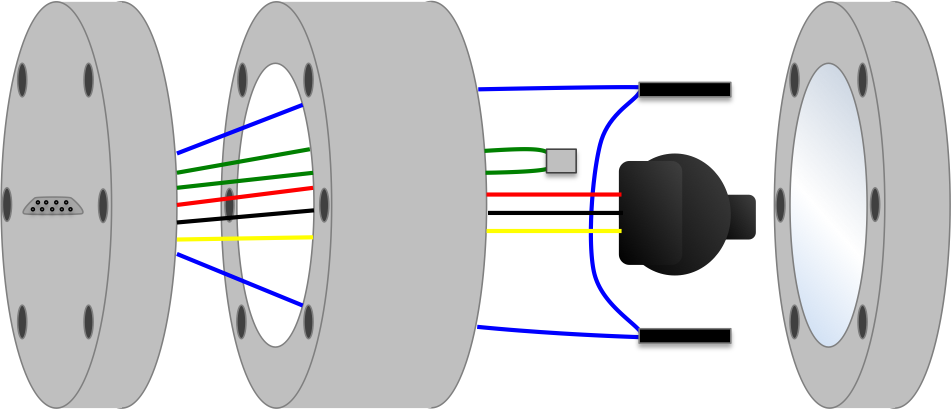
\includegraphics[width=\textwidth]{cam_in_housing_diagram}
    \caption{A schematic of the camera module.}
  \end{subfigure}
  \hspace{0.08\textwidth}
  \begin{subfigure}{0.45\textwidth}
    \centering
    \includegraphics[width=\textwidth]{camera_module_explode_labels}
    \caption{A sealed camera module, along with the components contained inside the module.}
  \end{subfigure}
  \caption[The components which made up a camera module used in the 35 ton camera system]
          {The components which made up a camera module used in the 35 ton camera system. Left shows a schematic representation of the components in the camera modules, with wires from the PT100 temperature sensor (green), the heating resistors (blue) and camera (red, blue, yellow), connected to a 9-pin D-sub feed through, shown on the left of the image. Right shows the physical components, both inside and outside, a module. A camera, a heater and a temperature sensor, can all be seen. A PTFE holder is used to ensure that the components remain in the desired locations, with the camera pressed up to the glass viewing panel. Bolts are used to ensure that the camera modules are leak tight.}
  \label{fig:CamModule}
\end{figure}

It was necessary to mount the camera modules inside the 35 ton. This was achieved using a custom-designed mounting bracket, an example of which is shown in Figure~\ref{fig:CamMount}. The mounts were fixed to existing cryogenic pipework, and could be freely rotated, so that the cameras could be pointed towards specific regions of interest. This meant that the camera mounts had two degrees of freedom, as well as being able to freely placed on the cryogenic pipes. \\

\begin{figure}[h!]
  \centering
  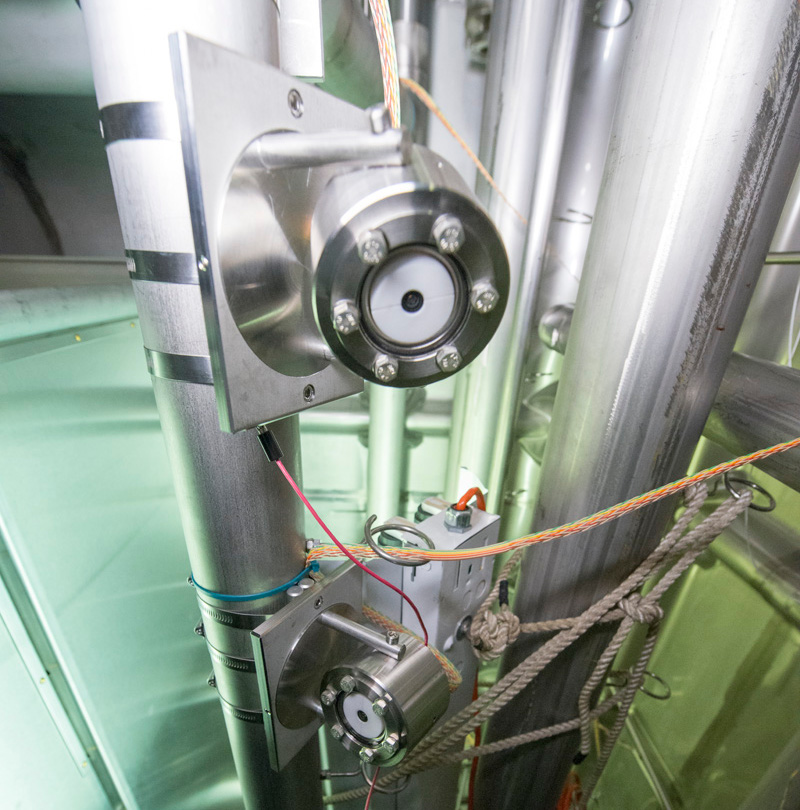
\includegraphics[width=0.45\textwidth]{cammount35tcrop}
  \caption[Two camera modules which are mounted in the 35 ton prototype detector]
          {Two camera modules which are mounted in the 35 ton prototype detector. The mounts are affixed to a 3'' SCH cryogenic pipe. The multi-coloured ribbon cables which were used to carry the camera signals outside of the cryostat can be seen in the picture.}
  \label{fig:CamMount}
\end{figure}

However, before the cameras could be installed in the 35 ton cryostat, several safety reviews had to be completed, in order to comply with safety standards set out by Fermilab, the host lab for the 35 ton prototype. This consisted of a review of the cable rack which was used during operations, plus individual reviews for the components which were custom-built. There was also a further review covering the camera system as a whole when it was operational. Only after the successful completion of all of these reviews was the camera system allowed to be installed, and ran unsupervised, inside the 35 ton cryostat. \\

In order to satisfy the safety requirements, adequate grounding of the rack, and all of its components, had to be displayed. This requirement extended to ensuring that the cables used in the system, which were assembled at Fermilab, would not introduce any potential ground loops into the 35 ton system. This meant that detailed diagrams of the individual components, and how they linked together to form the camera system, had to be produced. The detailed diagram which was produced representing the entire camera system is shown in Figure~\ref{fig:CamSysDiagram}. \\

\begin{figure}[h!]
  \centering
  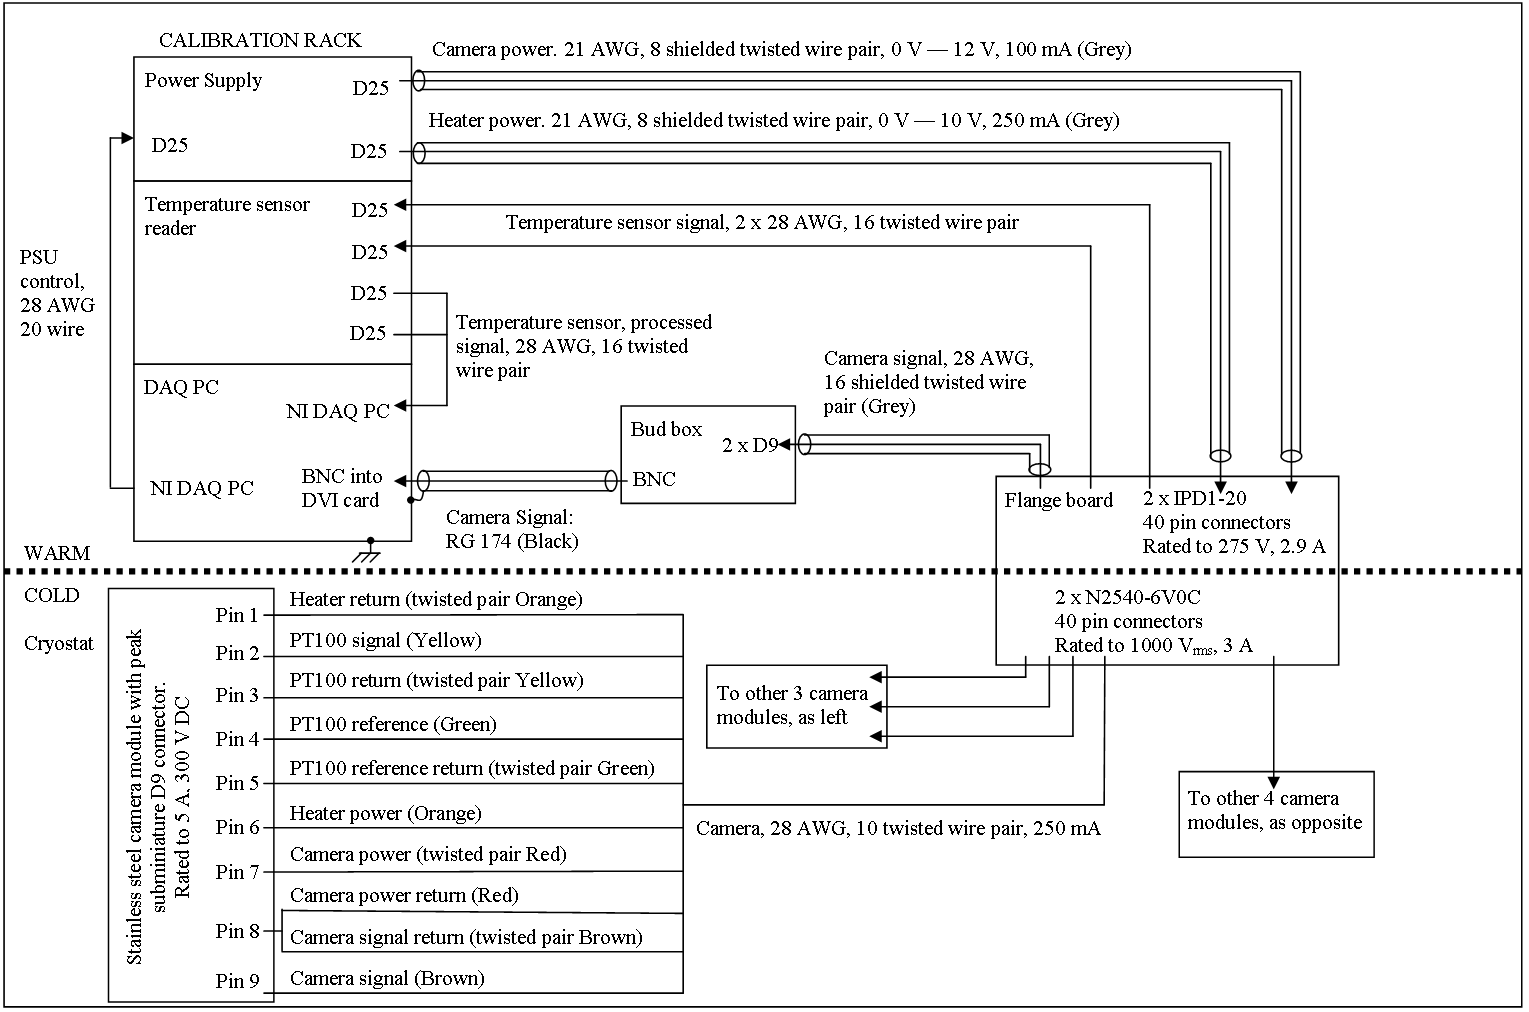
\includegraphics[width=0.95\textwidth]{Camera_Block_diagram}
  \caption[The system diagram for the 35 ton camera system]
          {The system diagram for the 35 ton camera system. The contents of the rack which was used in the camera system (top left), the wires which were terminated at the flange board (right), and the signals that each of the wires connected to the cameras carried (bottom left), are shown. In addition to this, the wire gauge (in units of AWG), along with the voltages and currents which they carried, and the number of wires which were bound together, are shown for the connections between each subsystem and the flange board. Shielded wires are shown as wires with cylindrical covers around them, such as the wire labelled ``Camera power.'' In total there were eight camera modules installed in the cryostat, connected in two groups of four cameras, to the flange board by two 40 pin connectors.}
  \label{fig:CamSysDiagram}
\end{figure}

%********************************** % Fifth Section  *************************************
\section{Performance in the 35 ton}  %Section - X.5
In total eight cameras were installed inside the 35 ton cryostat, the locations of which were selected to maximise the potential of observing any HV breakdowns which may occur. It was decided that the cameras would be focused on the following parts of the detector;
\begin{itemize}
\item The top right hand corner of the cathode.
\item The bottom right hand corner of the cathode.
\item The top left hand corner of the cathode.
\item The bottom left hand corner of the cathode.
\item The location of the high voltage feed through.
\item The ullage - the gap between the top of the TPC, and the roof of the cryostat
\item The cool down sprayers - this was only for use doing cool down, to check that they were operating as expected.
\item The phase separator - this was for use during operation to ensure that it was running as expected.
\end{itemize}
Upon installation in the cryostat, some calibration images were taken for each camera, these are shown in Figure~\ref{fig:CamFOV}. \\

\begin{figure}
 \centering
 \minipage{0.4\textwidth}
   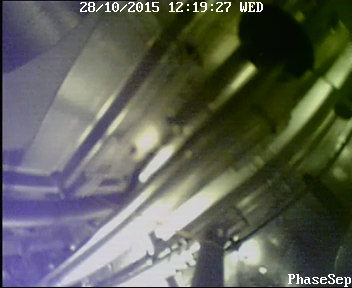
\includegraphics[width=\linewidth]{phasesep}
 \endminipage
 \minipage{0.4\textwidth}
  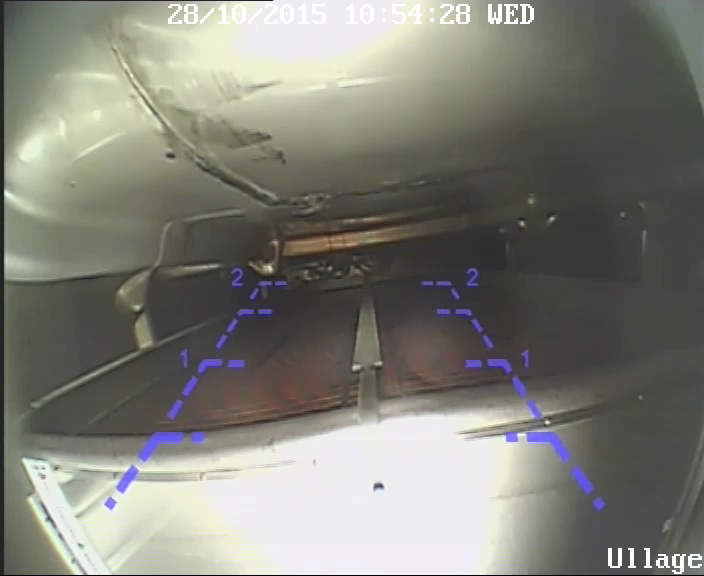
\includegraphics[width=\linewidth]{ullage}
 \endminipage

 \minipage{0.4\textwidth}
  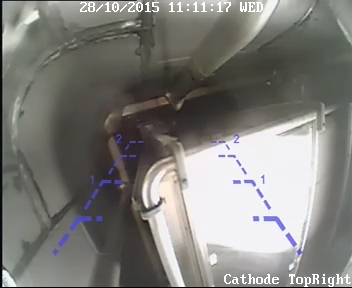
\includegraphics[width=\linewidth]{cathodetr}
 \endminipage
 \minipage{0.4\textwidth}
   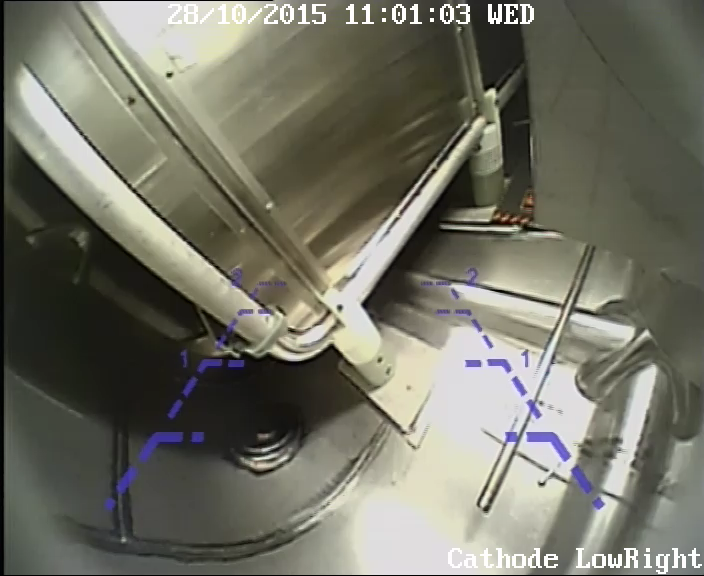
\includegraphics[width=\linewidth]{cathodelr}
 \endminipage

 \minipage{0.4\textwidth}
   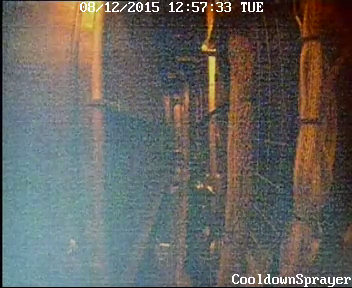
\includegraphics[width=\linewidth]{cooldownsp}
 \endminipage
 \minipage{0.4\textwidth}
   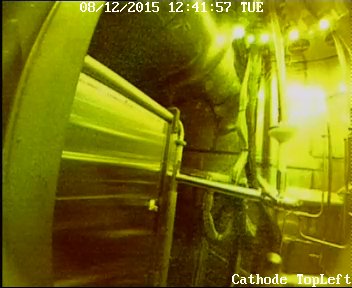
\includegraphics[width=\linewidth]{cathodetl}
 \endminipage

 \minipage{0.4\textwidth}
   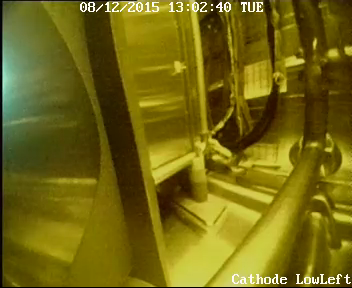
\includegraphics[width=\linewidth]{cathodell}
 \endminipage
 \minipage{0.4\textwidth}
   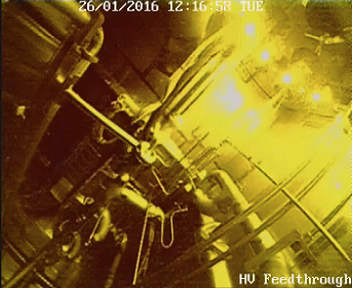
\includegraphics[width=\linewidth]{hvft}
 \endminipage
 \caption[The calibration images for the 8 cameras used in the 35 ton camera system]
         {The calibration images for the 8 cameras used in the 35 ton camera system.  The images from left to right, top to bottom, show the following: phase separator, ullage, cathode top right, cathode bottom right, cool down sprayers, cathode top left, cathode bottom left, and high voltage feed through.  The upper four images were taken with a halogen light illuminating the cryostat, prior to it being sealed up.  The lower four images were taken with an LED ring light on, with the cryostat sealed up.  All images are left-right inverted due to software.}
 \label{fig:CamFOV}
\end{figure}

As previously mentioned, the cameras used were car reversing cameras, and so this is why there are distance lines on some of the images in Figure~\ref{fig:CamFOV}. From Figure~\ref{fig:CamFOV}, it also evident that there is a large variation in the picture quality of the different cameras. This is attributed to aspects of the cabling, as some cables were slightly longer than others, or had less reliable electrical connections. It could also be due to differences in the cameras, because, as discussed in Section~\ref{sec:CamDesign}, the stability of the cameras which were tested was not uniform. This variability in the camera stability, also manifested itself in the amount of signal degradation which was observed over time. The signal degradation over the course of the run, for two cameras, is shown in Figure~\ref{fig:CamSigDeg}. \\

\begin{figure}[h!]
  \centering
  \begin{subfigure}{0.95\textwidth}
    \centering
    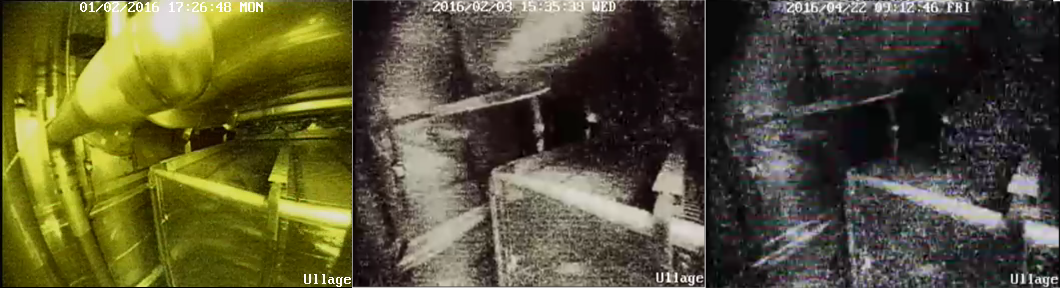
\includegraphics[width=\textwidth]{Cam1degradation2}
    \caption{The degradation in signal quality of the camera focused on the ullage.}
  \end{subfigure}
  \begin{subfigure}{0.95\textwidth}
    \centering
    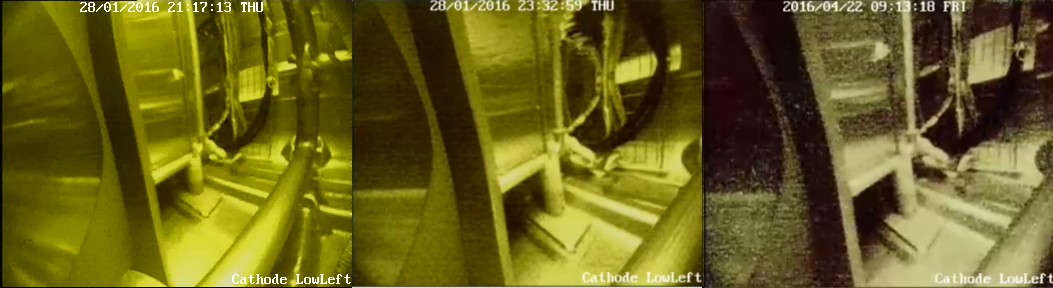
\includegraphics[width=\textwidth]{Cam4degradation2}
    \caption{The degradation in signal quality of the camera focused on the lower left corner of the cathode.}
  \end{subfigure}
  \caption[The signal degradation over time for two cameras in the 35 ton camera system]
          {The signal degradation over time for two cameras in the 35 ton camera system. Top shows the signal degradation observed for the camera focused on the ullage. Bottom shows the signal degradation for the camera focused on the lower left corner of the cathode. For both cameras, left shows the field-of-view prior to cool down, centre shows the field-of-view immediately after cool down, and right shows the field-view after 10 weeks of operation. These are full colour images, as recorded by the DVR, and so no post-processing has been performed on the images.}  
  \label{fig:CamSigDeg}
\end{figure}

From Figure~\ref{fig:CamSigDeg}, it can be seen over the course of the run, the fields-of-view for both cameras became more pixelated, and that there was an increase in the number of pixels which were either saturated, or dead. The large number of saturated pixels was particularly evident when the cryostat was not illuminated, and meant that the region which could be used to trigger on HV breakdowns was severely limited for some cameras. As shown, this degradation was highly camera specific, with the resolution of the ullage camera deteriorating severely, whilst the camera focusing on the lower left corner of the cathode is relatively unchanged over the course of the run. A striking difference between the left-most images, and the central and right-most images, in Figure~\ref{fig:CamSigDeg}, is the loss of colour in the images which are produced. This is attributed to a partial failure of the on-board encoding circuits, which resulted in the colour signal streams not being functional when exposed to cryogenic temperatures. This loss of colour was seen as soon as the cameras were exposed to cryogenic temperatures, and was also observed in the initial tests performed in Sheffield. \\

During normal operation of the 35 ton system, the high voltage operated stably at 60 kV, and so no breakdowns were observed. However, after the cathode was raised to 135 kV in low-purity argon, three of four breakdowns were detected by the camera system, and data was written to disk as expected. Unfortunately, the cameras were not able to pinpoint the exact locations of the breakdowns, and so their effectiveness at discerning the locations of HV breakdowns is still largely untested. Despite this, however, the cameras proved to be a very valuable monitoring tool in the 35 ton cryostat, and there has been interest in including analogous systems in future LArTPCs, such as SBND~\citep{SBNProposal}. \\

It is also important to note that the cameras were able to operate safely within their modules, and did not impinge on any other systems in the cryostat. They were also found to be able to be power cycled after large periods of time in the cold, including after not being operational for a large period of time. One such period, which lasted for 9 days, was when the cameras were powered off whilst extensive noise hunting was performed. Upon being power cycled, all 8 cameras were immediately brought back online, without the need for the inbuilt heaters. \\

%*****************************************************A**************************
%********************************** Chapter XXXXXXXX ***************************
%*******************************************************************************

\nomenclature[z-MIP]{MIP}{Minimally Ionising Particle}
\nomenclature[z-MPV]{MPV}{Most Probable Value} 
\nomenclature[z-PID]{PID}{Particle IDentification}
\nomenclature[z-ROI]{ROI}{Region Of Interest}

\chapter{Simulations of the 35 ton prototype}  %Title of chapter

\graphicspath{ {35tonSimulation/Figs/PDF/} {35tonSimulation/Figs/Vector/} } %{35tonSimulation/Figs/Raster/}

%********************************** %First Section  *************************************
\section{Determination of interaction times} \label{sec:SimInteractionTimes} %Section - X.1
As outlined at the end of Section~\ref{sec:LArSoft} it is important to know the interaction time of a track when performing calorimetric reconstruction. When performing simulations the simplest interaction time to assign to a reconstructed object is the Monte Carlo truth time of when the particle was created. The creation time can be used as the distances considered in simulations are small compared to the velocities which the particles are initially travelling meaning that interactions throughout the volume are less than the resolution of the detector (500 ns). When matching a reconstructed object with a GEANT4 particle the particle which contributed the most overall deposited charge to the whole track is chosen. This means that the energy deposited for each hit on the track is broken down into how much each particle contributed to the charge of the individual hit, with the energies summed over all hits. The ability to assign the true interaction times to 3D objects is vital when wanting to benchmark how well other determinations of interaction times perform or to determine the efficiency of the tracking algorithms as described in Section~\ref{sec:SimRecoEffic}. \\

In the 35 ton detector, it was envisioned that there would be at least two ways in which interaction times could be assigned to tracks, one using the external cosmic ray counters and another using reconstructed scintillation light collected by the photon detectors. The cosmic ray counters were used extensively in the 35 ton data, as described in Section~\ref{sec:DataAlgs}, however in simulation the scintillation light was used as this would have been more powerful during continuous running as not all particles would pass through counters but one wold expect almost all of them to produce reconstructable scintillation light. Flashes of lights are reconstructed by using a pre-built library which models the expected number of photoelectrons to be measured on each photon detector given the 3D position of the source of the flash. This library takes into account the expected quantum efficiencies of each photon detector. \\

When trying to produce an association metric a sample of 10,000 Anti-Muons with a cosmic-like distribution was used as then there there should only be one long track with which to match one reconstructed flash. A cosmic-like distribution is defined as a set of particles which have a $\cos^{2}$ angular distribution, no minimum or maximum energies and have a flat distribution of initial positions in the $xz$ plane and a uniform initial $y$ position. When this sample was simulated it was clear that the photon detector reconstruction using the pre-built libraries worked well as the reconstructed flash source normally lay very close to the track which caused it. It was found that a calculation of a Point Of Closest Approach (PoCA)!!~citep{PoCA}!! of the reconstructed track to the flash source gave an effective metric by which the two could be combined. Other metrics such as the distance between the flash source and the track centre, and the perpendicular distance between the flash source and the line joining the start and end of track were investigated but found to provide a less reliable metrics. The latter of these metrics is less effective because the reconstructed tracks are rarely straight lines, due to particles scattering as they travel through the LAr and so the perpendicular distance at each hit must be calculated. A comparison of these metrics is shown in Figure~\ref{fig:PDYZDist}. \\

\begin{figure}[h!]
  \centering
  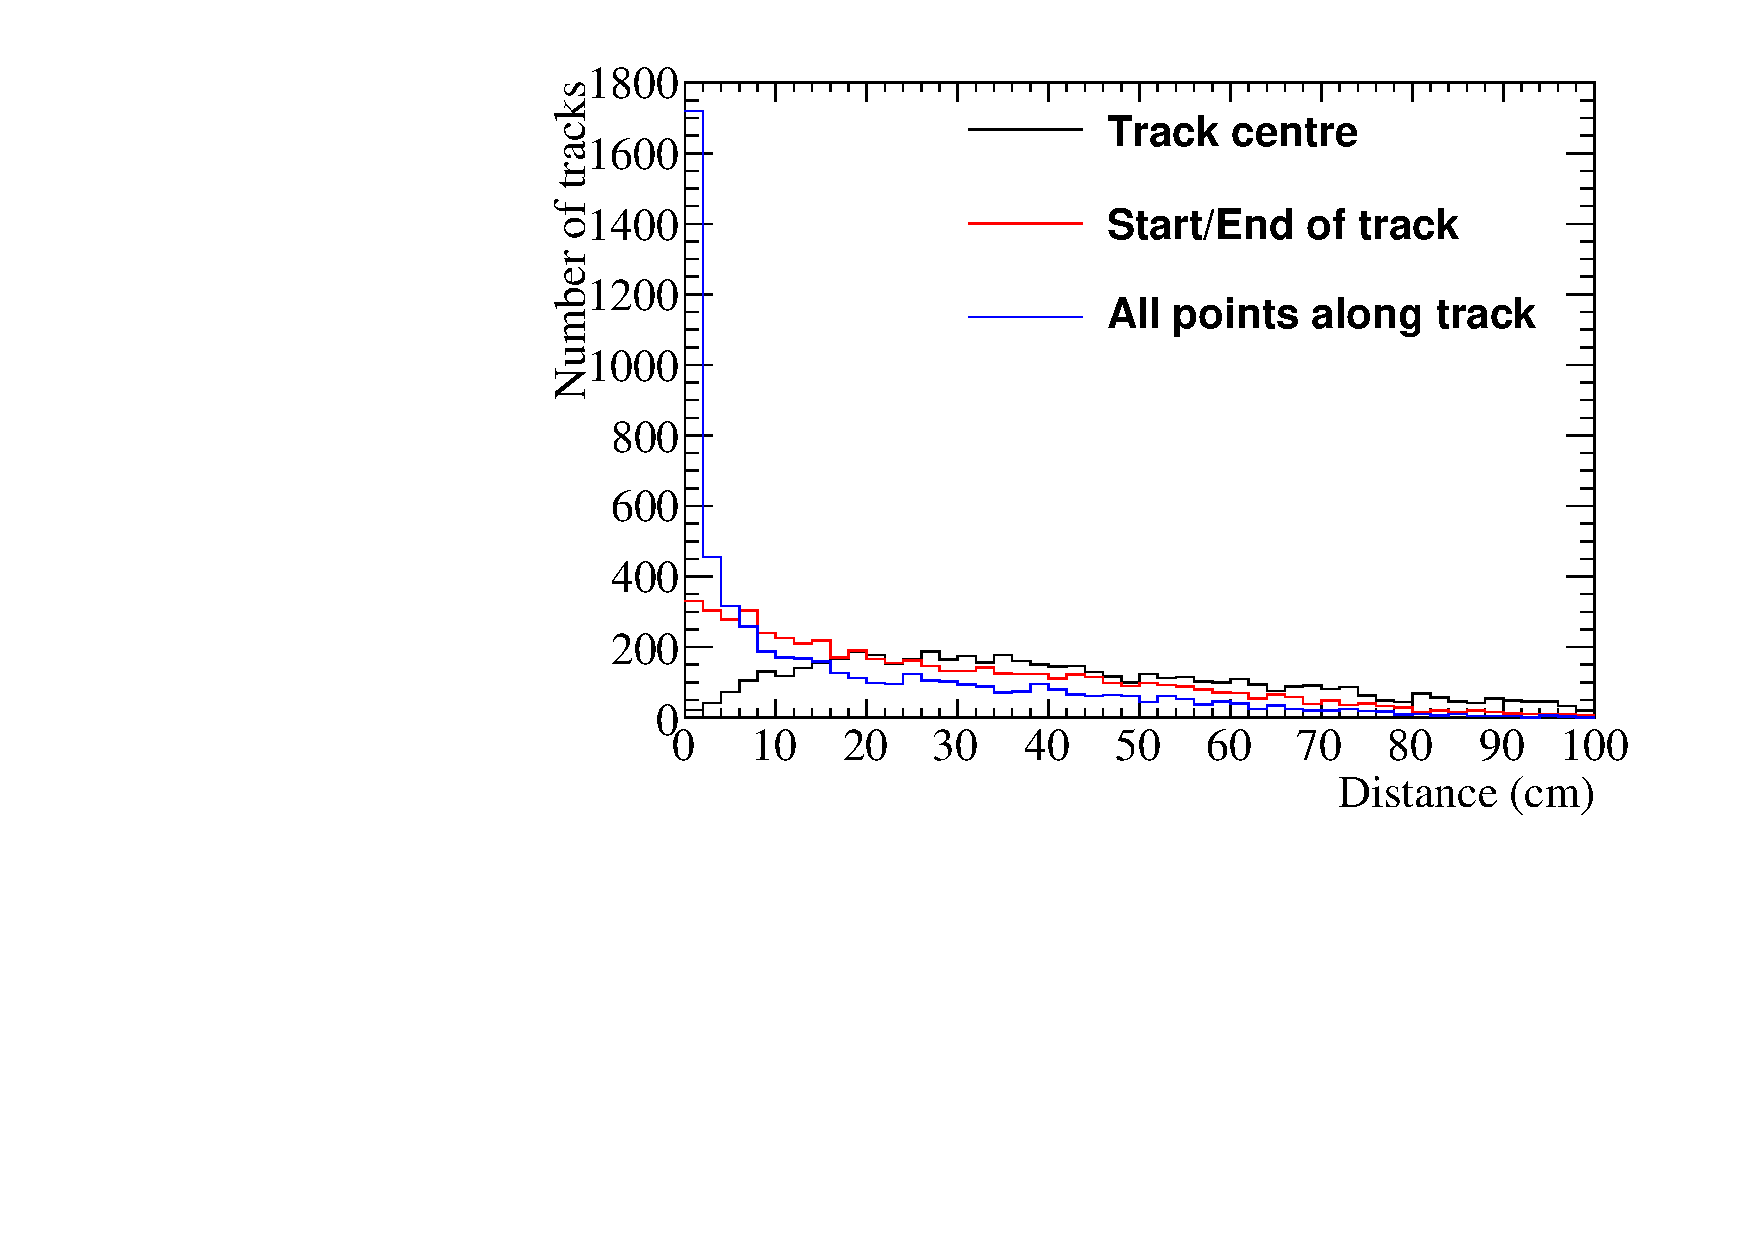
\includegraphics[width=0.5\textwidth]{DiffTrackSeps}
  \caption[Matching tracks and flashes in the 35 ton using positions in the $yz$ plane]
          {A comparison of $yz$ comparisons of reconstructed tracks and flashes in the 35 ton.}
  \label{fig:PDYZDist}
\end{figure}

Another metric by which flashes could be assigned to reconstructed tracks is by utilising the relationship between the number of measured photoelectrons and the distance from the APAs at which they were produced. When considering two flashes of scintillation light that are produced at different distances from the APAs, it would be expected that more photoelectrons would be collected from the photons produced closer to the APAs. Utilising this relationship, shown in Figure~\ref{fig:PD_PExPlot}, means that the distance from the APAs can be predicted from the number of photoelectrons which are measured. This predicted distance can then be compared to the expected $x$ position of a reconstructed track given the difference in flash time and hit times, this is shown in Figure~\ref{fig:PD_PEDiffX}. The difference in these two quantities is used as the second metric as it gives an indication of how well a flash properties match the reconstructed $x$ position of the track, with a value of 0 representing an excellent match. \\

\begin{figure}[h!]
  \centering
  \begin{subfigure}{0.45\textwidth}
    \centering
    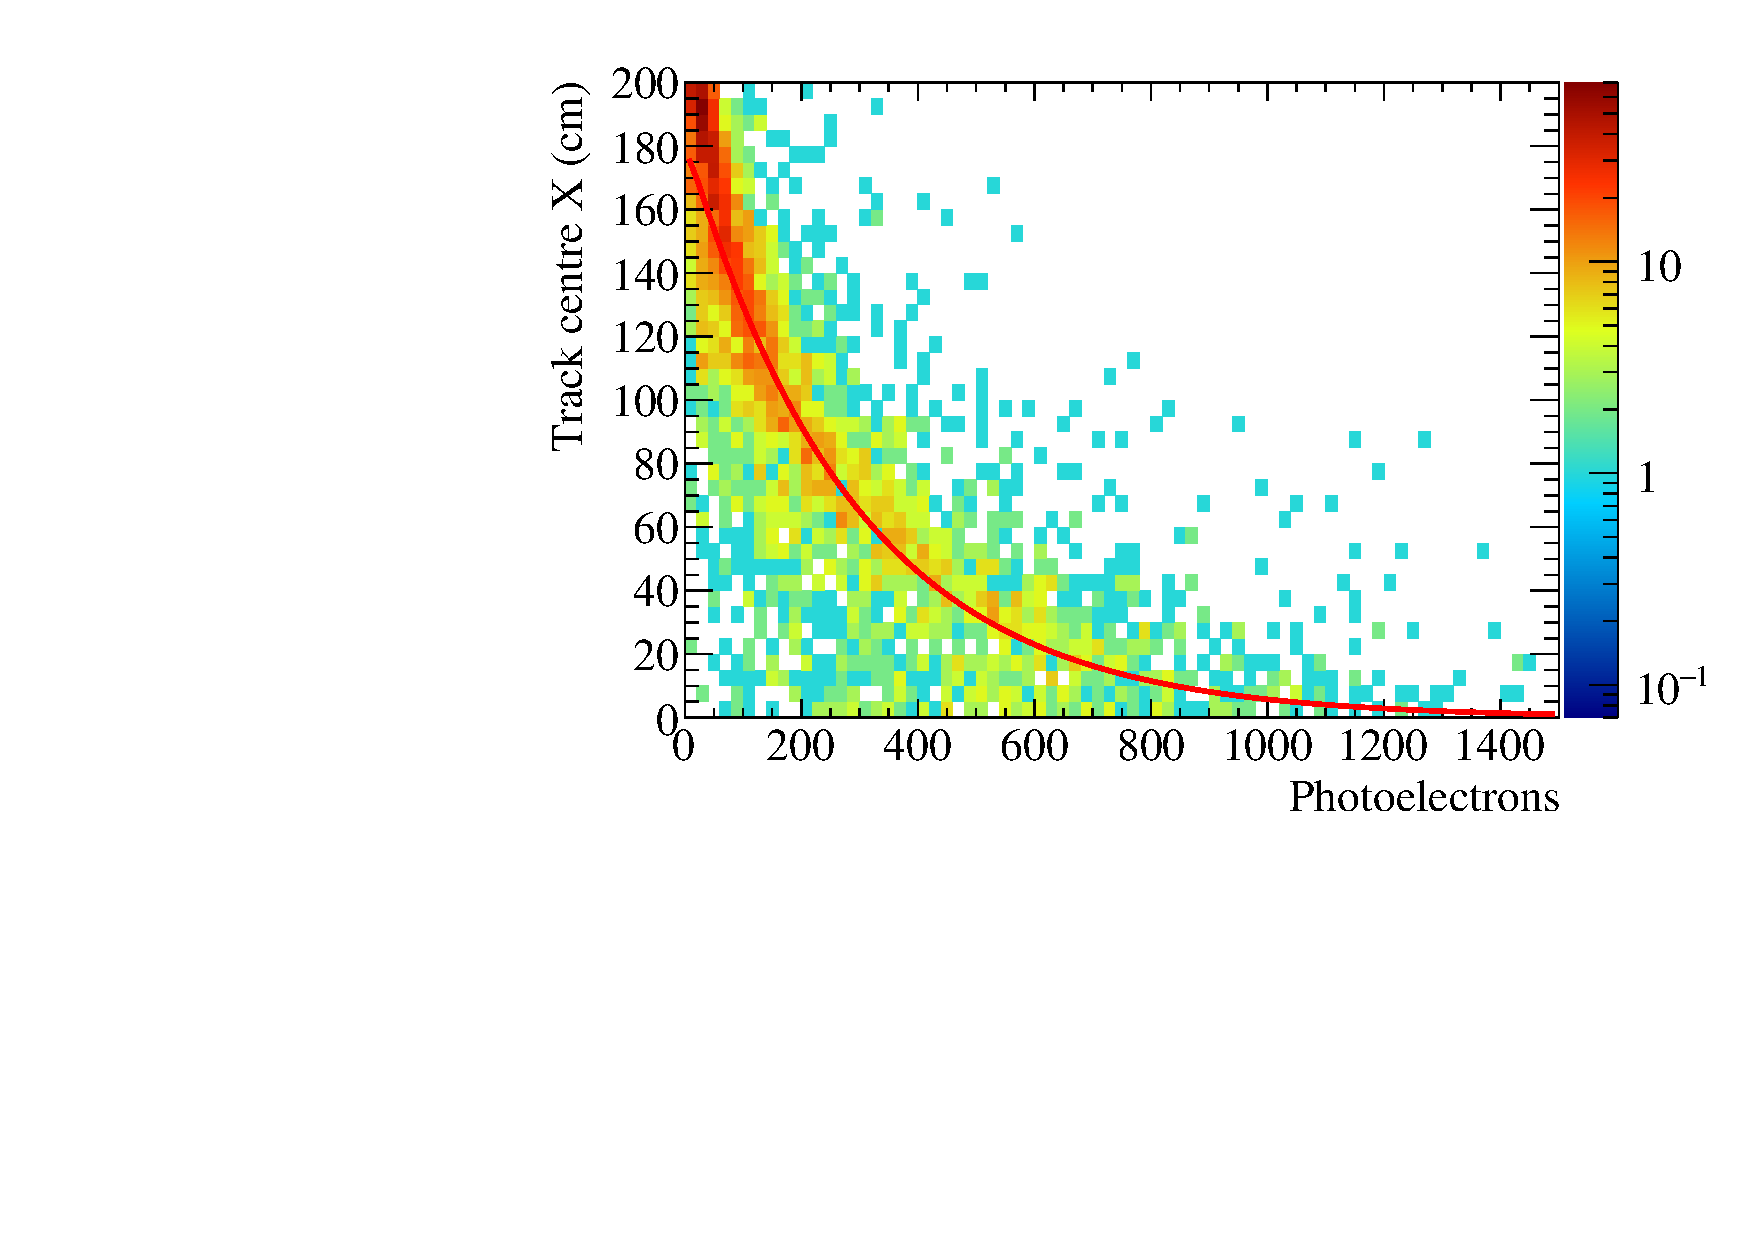
\includegraphics[width=\textwidth]{NumPE_Distance}
    \caption{How the number of photoelectrons measured changes with drift distance.}
    \label{fig:PD_PExPlot}
  \end{subfigure}
  \hspace{0.08\textwidth}
  \begin{subfigure}{0.45\textwidth}
    \centering
    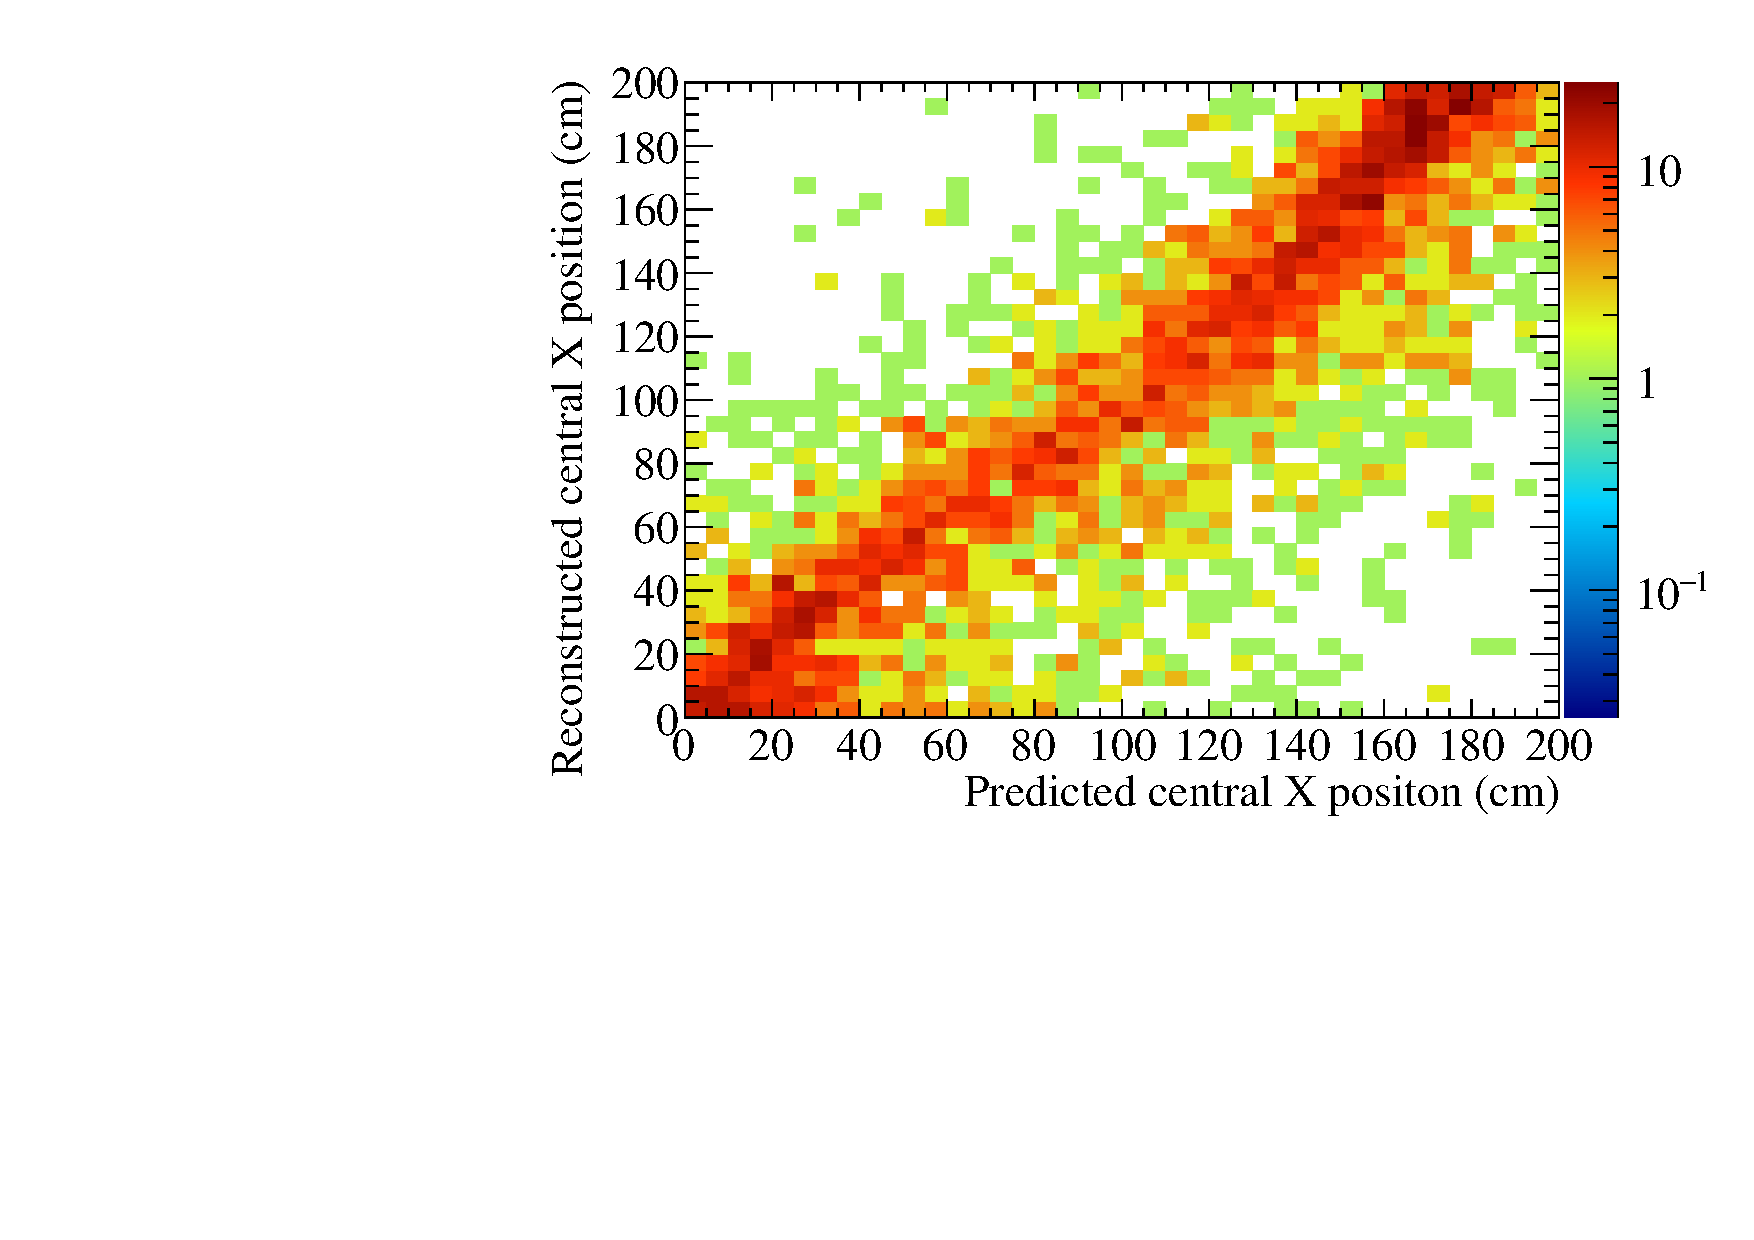
\includegraphics[width=\textwidth]{DiffFlashPredReco}
    \caption{The difference in $x$ position using the relationship in Fig~\ref{fig:PD_PExPlot} and the difference in flash and hit times.}
    \label{fig:PD_PEDiffX}
  \end{subfigure}
  \caption[Matching tracks and flashes in the 35 ton using photoelectron information]
          {How the number of reconstructed photoelectrons changes with increasing drift distance, and how this can be used to predict the interaction time of tracks. How consistent the predicted interaction times using this method replicate the $x$ positions one would expect given the drift times they correspond to, there is one entry for every track/flash pair.}
\end{figure}

Using these metrics it is possible to attempt to assign reconstructed flashes to reconstructed tracks. Only flashes which are within one drift window of a given track are considered, as flashes outside of this time window cannot have been caused by the reconstructed track. Once flashes are assigned to tracks it is possible to determine how well the matching has performed by comparing the Monte Carlo truth interaction time with the photon detector interaction time. When doing this it is more useful to use a long (16 ms, 32,000 tick) CRY sample as then particles come at random timings as opposed to all at $T$ = 0 as with the Anti-Muon sample initially considered. This comparison is shown in Figure~\ref{fig:PD_MCPDDiff}, where there is a clear peak at a time difference of 0 ms in the Monte Carlo truth and photon detector interaction times. When zooming in on this peak it can be seen that there is a systematic offset of 0.6 $\mu$s, this is due to an electronics offset applied in the simulation to the photon detector system. \\

\begin{figure}[h!]
  \centering
  \begin{subfigure}{0.45\textwidth}
    \centering
    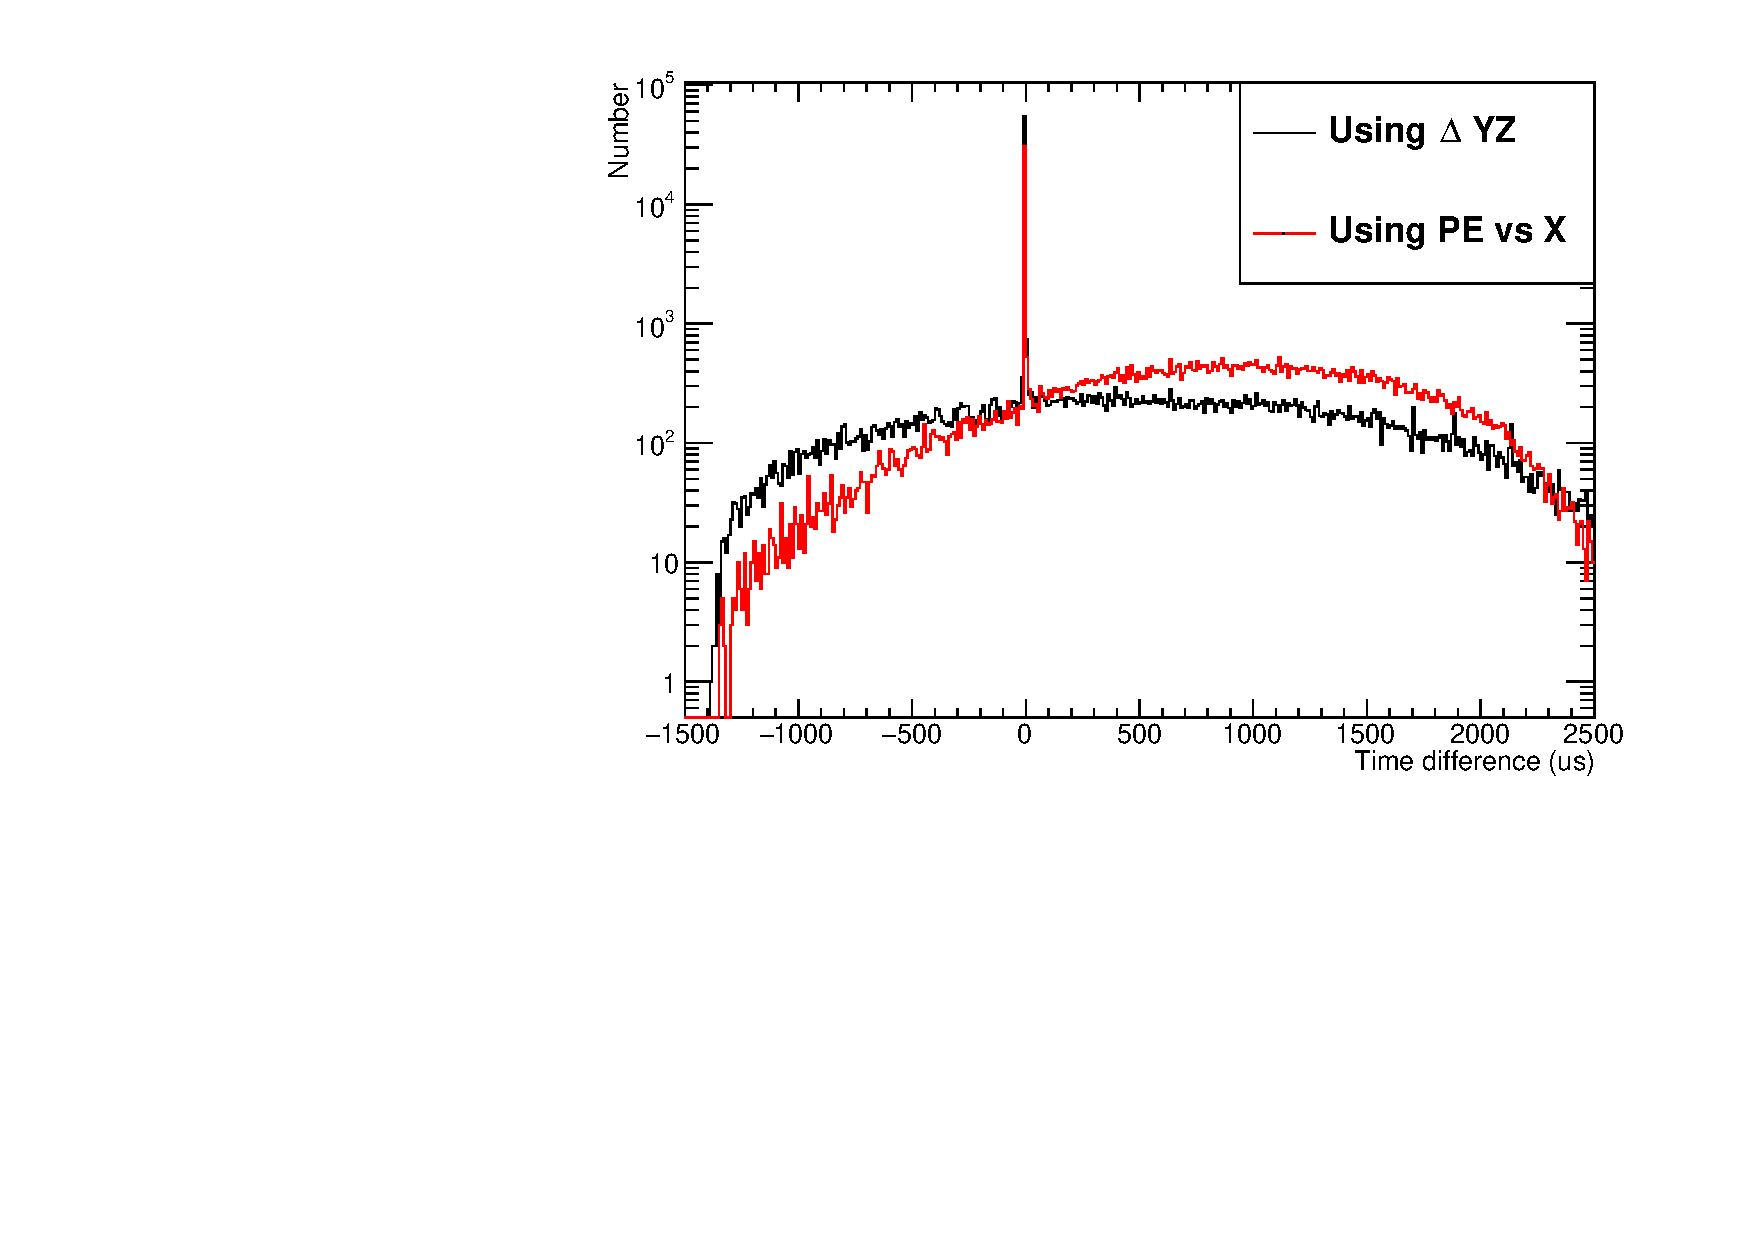
\includegraphics[width=\textwidth]{Pred_Reco_T_Full}
    \caption{The difference in interaction times.}
  \end{subfigure}
  \hspace{0.08\textwidth}
  \begin{subfigure}{0.45\textwidth}
    \centering
    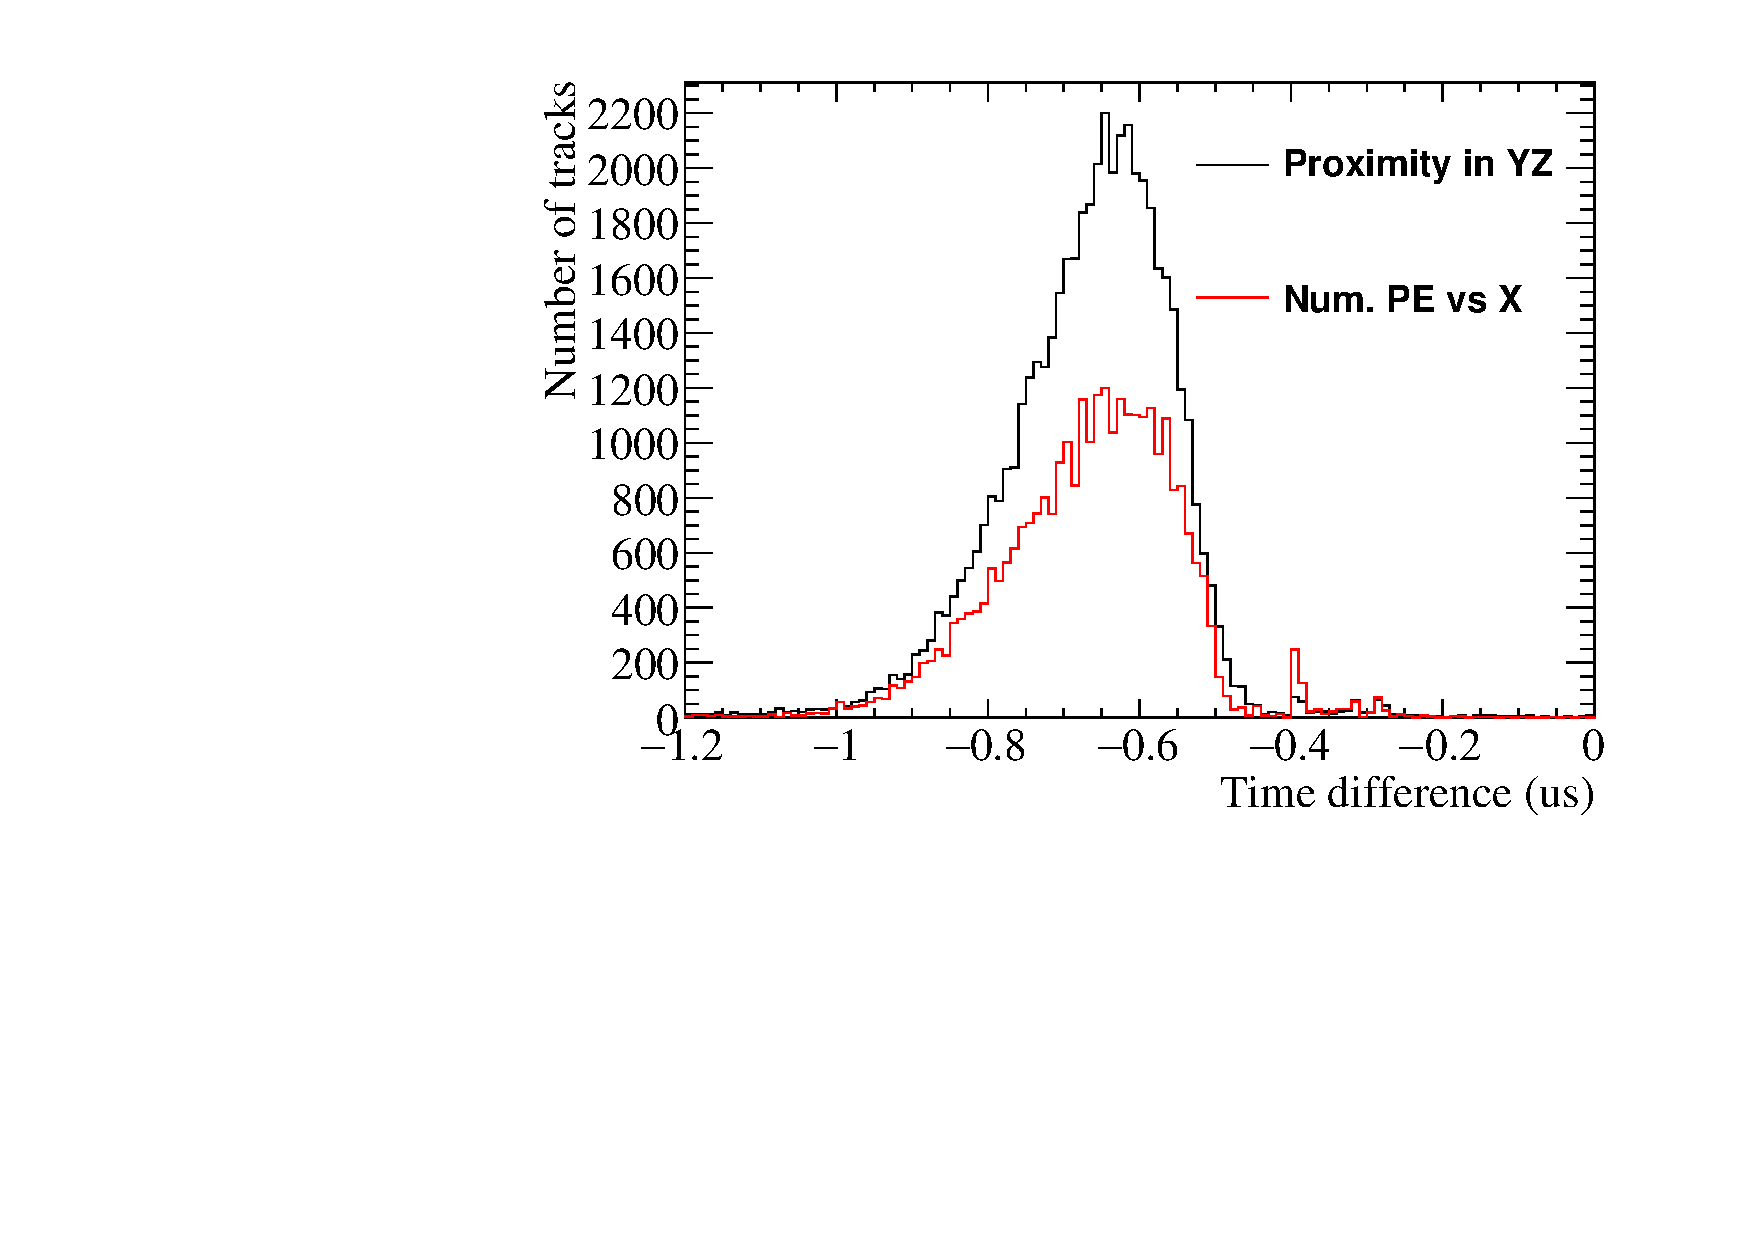
\includegraphics[width=\textwidth]{Pred_Reco_T_Zoom}
    \caption{Zoomed in at low time differences.}
  \end{subfigure}
  \caption[The difference in Monte Carlo interaction times and the predicted interaction times using the photon detectors]
          {The difference in Monte Carlo interaction times and the predicted interaction times using the photon detectors.}
          \label{fig:PD_MCPDDiff}
\end{figure}

From Figure~\ref{fig:PD_MCPDDiff} it can clearly be seen that the metric using the proximity of the flash centre to the track trajectory yields the best matches. This is likely caused by the large spread in the number of photoelectrons collected at fixed drift distances, as shown by Figure~\ref{fig:PD_PExPlot}. The two metrics can be combined to give a prediction for the interaction time, though given the increased sensitivity from the proximity metric this should be given greater weighting. In physics data the metric using the number of collected photoelectrons is particularly sensitive to the absolute light level in the detector as a high residual light level would reduce the proportional change in the number of photoelectrons collected for increasing drift distances. This metric also relies a sample of tracks with known $x$ positions upon which it can be calibrated which may be difficult to obtain. \\



%********************************** % Second Section  *************************************
\section{Calibrating calorimetric constants} \label{sec:MCCalib} %Section - X.2
Having the correct calorimetric responses is vital when trying to calculate $\frac{dE}{dx}$ as the measured change in charge has to be correctly converted to the change in energy. The parameters which need to be tuned in order to ensure that this is done correctly are the $Recomb_A$ and $Recomb_B$ of Equations~\ref{eq:ModBox},~\ref{eq:ModBox_B},~\ref{eq:Birks_A} and~\ref{eq:Birks_B} respectively. These parameters have to be tuned in such a way as to make a known particle energy deposition have the correct $\frac{dE}{dx}$, the easiest deposition to tune against is the Minimally Ionising Particle (MIP) peak which in LAr should have a value of 1.8 MeV cm$^{-3}$. To do this the sample of 10,000 Anti-Muons made to calibrate the photon detector track/flash assignment will be used as many of these particles will be MIPs. \\

To select the MIPs in the sample only tracks caused by through-going muons are used. The $\frac{dE}{dx}$ value for all hits in all tracks is then calculated, with the different planes separated out as each one will have its own normalisation factor. A Gaussian distribution is then fitted around the peaks for each of the planes to discern the Most Probable Value (MPV) of $\frac{dE}{dx}$ for that plane. If the MPVs are not equal to 1.8 MeV cm$^{-3}$ then the normalisation factors are scaled through a process of trial and error until the correct MPVs are measured. An example of the tuning being applied is shown in Figure~\ref{fig:CaloTune}. Tuning of the calorimetric constants is required whenever the electronics gains or signal shaping functions are changed.

\begin{figure}[h!]
  \centering
  \begin{subfigure}{0.45\textwidth}
    \centering
    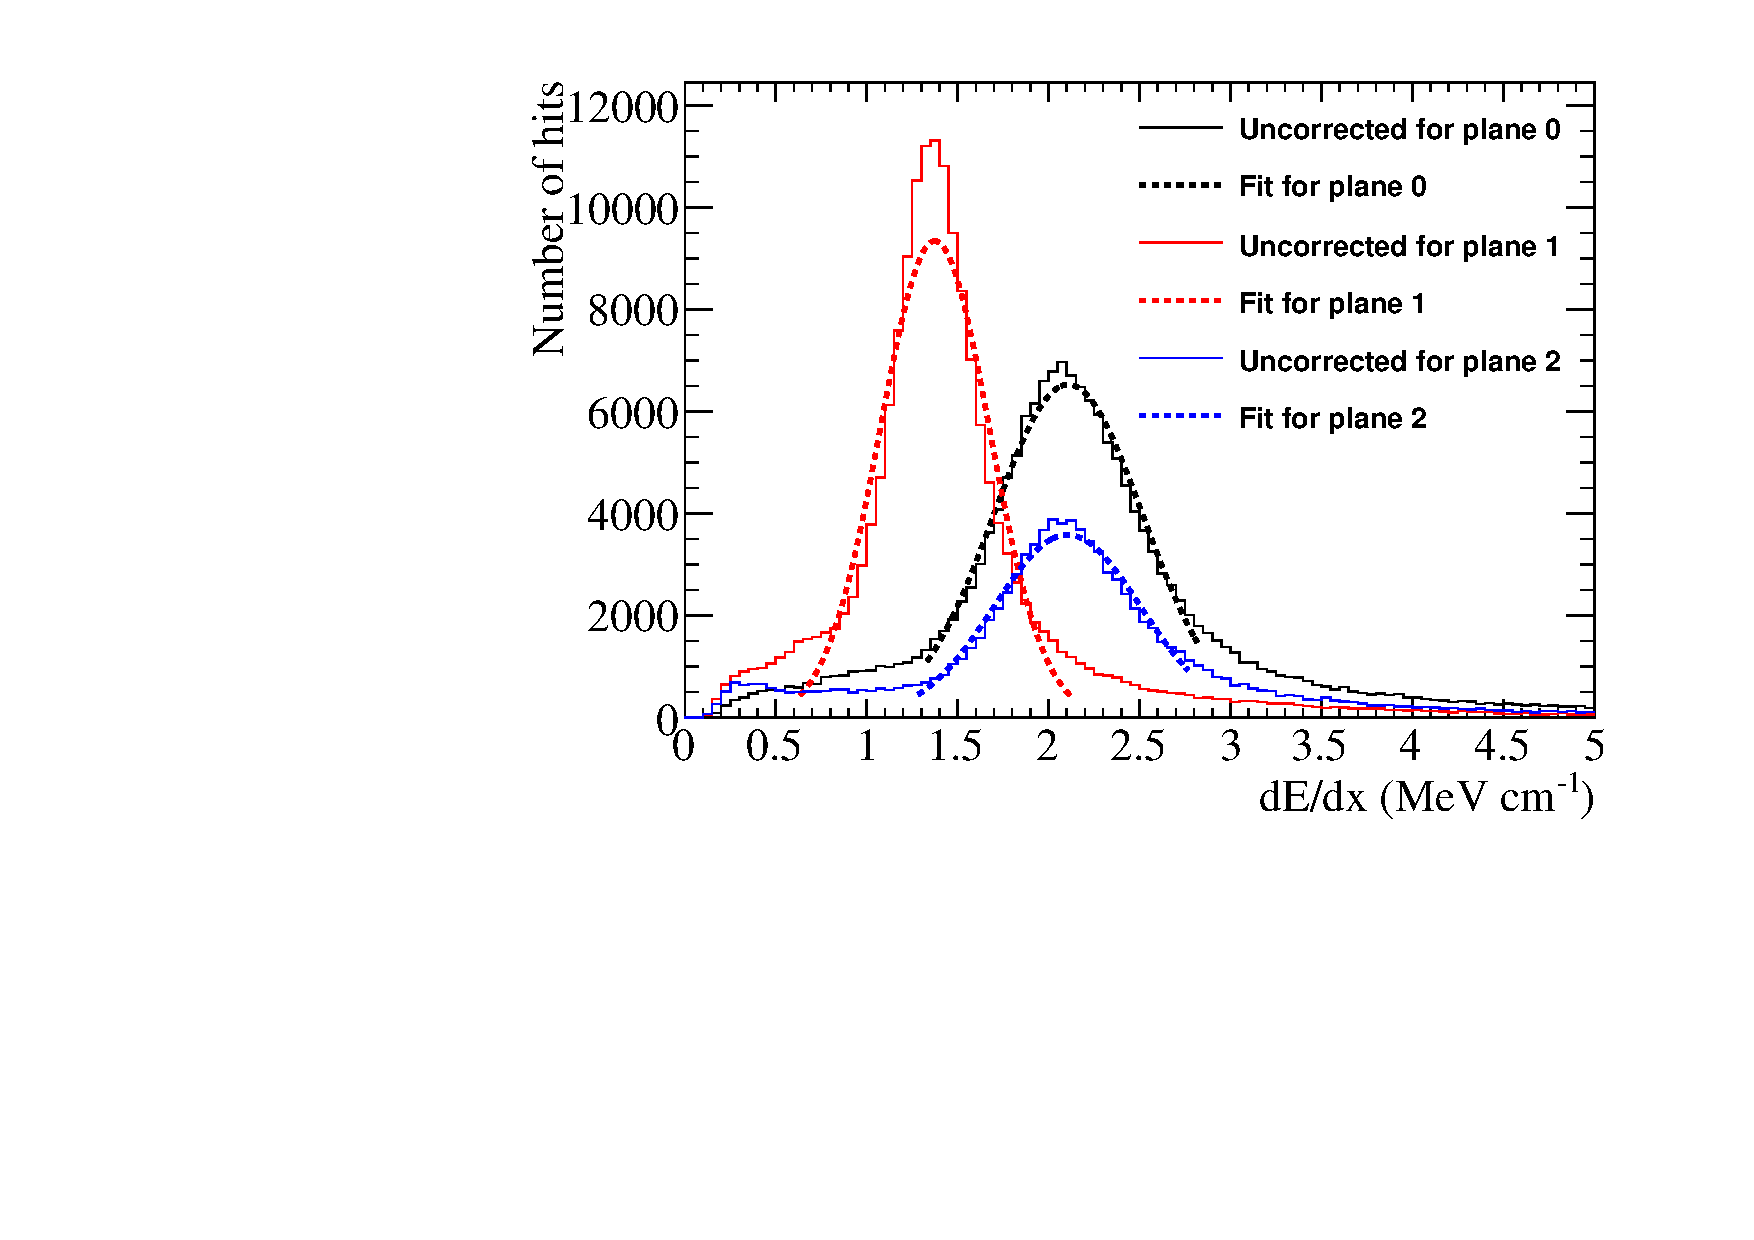
\includegraphics[width=\textwidth]{UnCorrectedCanvas}
    \caption{Before a normalisation correction is applied.}
    \label{fig:CaloTune_Before}
  \end{subfigure}
  \hspace{0.08\textwidth}
  \begin{subfigure}{0.45\textwidth}
    \centering
    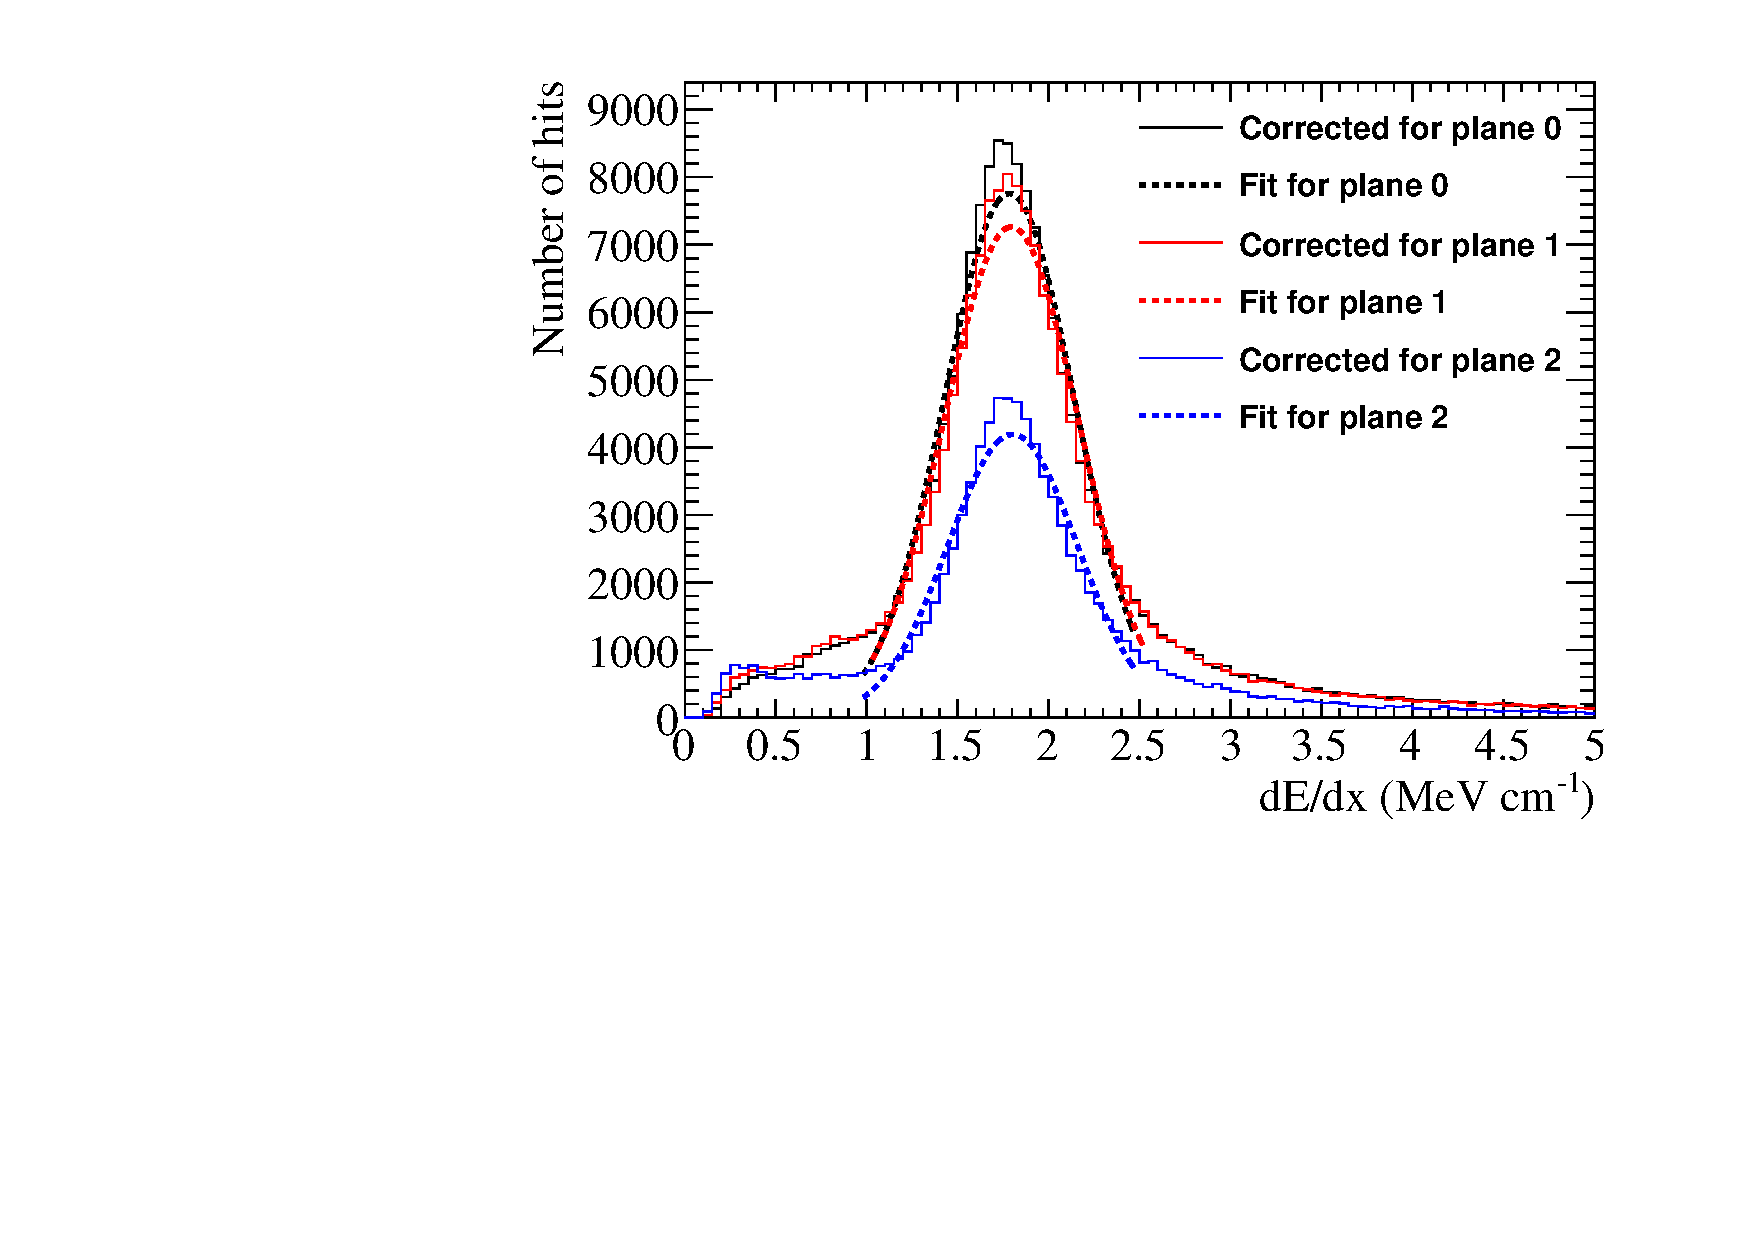
\includegraphics[width=\textwidth]{CorrectedCanvas}
    \caption{After a normalisation correction is applied.}
    \label{fig:CaloTune_After}
  \end{subfigure}
  \caption[The tuning of the calorimetric constants in the 35 ton]
          {How the $\frac{dE}{dx}$ MPVs change for each plane when a change is made to the electronics gains in the 35 ton. Figure~\ref{fig:CaloTune_Before} shows the MPVs after the change using the previous constants, whilst Figure~\ref{fig:CaloTune_After} shows the MPVs after a re-tuning of the constants.}
          \label{fig:CaloTune}
\end{figure}
        
%********************************** % Third Section  *************************************
\section{Discerning reconstruction efficiencies} \label{sec:SimRecoEffic} %Section - X.3
Knowledge of the strengths and weaknesses of different tracking algorithms is vital when using them for physics analyses, to this end it is useful to develop a metric by which they can be compared. In order to do this a series of conditions have to be applied to the reconstructed tracks from a large set of simulated particles which are reconstructed using different tracking algorithms. It is interesting to observe what the effect of event complexity has on the reconstruction algorithms and so efficiencies will be calculated for both the Anti-Muon and CRY samples used in Section~\ref{sec:SimInteractionTimes}. \\

The criteria upon which to determine whether a particle is well reconstructed has to be carefully chosen as every definition will have limitations. For example, consider a particle that travels 100 cm in the active volume of the detector but is reconstructed as 2 separate tracks (tracks 1 and 2), with lengths 77 cm and 23 cm respectively. Firstly, should these tracks should be merged, or left separate? If the reconstruction algorithms have found them to be separate tracks then it would be difficult to ascertain that they are from the sample particle in real data, and so in considerations here they are not merged. One metric of efficiency would be to consider a track well reconstructed if it has a length between 75$\%$ and 125$\%$ of the Monte Carlo truth length that the particle traversed in the detector, in which case track 1 would be considered well reconstructed. Another metric however would be to consider a track well reconstructed if the Monte Carlo truth distance the particle traversed in the detector is between 75$\%$ and 125$\%$ of the reconstructed length, in which case neither track would be considered well matched. Both metrics have used exactly the same tracks and a seemingly identical method of evaluating whether a track is well reconstructed or not, but have got the opposite results. As such it is wrong to say which consideration gives the correct result, but instead the result of each should be considered equally. In discussions here the former definition of efficiency will be used, such that a track is considered well reconstructed if:
\begin{itemize}
\item Reconstructed track length is more than or equal to 75$\%$ of the Monte Carlo track length.
\item Reconstructed track length is less than or equal to 125$\%$ of the Monte Carlo track length.
\item Only one reconstructed track can be matched per Monte Carlo particle.
\end{itemize}

When calculating efficiencies it is important to consider much more than just the ratio of reconstructed to true track length. To this end efficiencies with regards to many aspects of the tracks are calculated:
\begin{itemize}
\item Track length
\item Energy deposited in the active volume of the detector
\item The angle $\theta$ of the track
\item The angle $\phi$ of the track
\end{itemize}
In all efficiency plots the Monte Carlo truth quantity, not the reconstructed quantity is shown so as to reflect how the variations of these quantities affect the reconstruction efficiencies. It is also useful to observe the effect on reconstruction of failed disambiguation and incorrect interaction time determination. To show this two forms of reconstruction are ran on the particles, one no Monte Carlo information is used and another where the disambiguation and interaction time are cheated. Cheated disambiguation means using the Monte Carlo truth information of the energy deposition to correctly assign which wire segment the energy was deposited on. \\

The calculation of reconstruction efficiencies also serves as an effective method upon which reconstruction algorithms can be further developed as it identifies aspects which do not work as expected. For example when the efficiencies for the CRY sample were initially calculated they were significantly lower than for the Anti-Muon sample, but only when disambiguation was not cheated. It transpired that this was because the disambiguation was only selecting the largest collection of hits on each plane for each TPC. This is not a problem when only 1 particle is simulated and will reduce the number of noise hits but in a CRY sample of 16 ms there will almost certainly be multiple particles in each TPC. Removing the hits from all but one of these multiple particles will cause them to have no reconstructed track, and thus cause the efficiency to drop significantly. Upon making the disambiguation algorithm no longer have this restriction the reconstruction efficiencies of the Anti-Muon and CRY samples were observed to become much more similar. \\

The reconstruction efficiencies given the current state of the most commonly used reconstruction algorithms are shown in Figures~\ref{fig:SimEffic_Length},~\ref{fig:SimEffic_EnDepos},~\ref{fig:SimEffic_Theta},~\ref{fig:SimEffic_Phi} and~\ref{fig:SimEffic_ThetaPhi}. Efficiencies are shown for both the Anti-Muon and CRY samples, where it can be seen that the efficiency tends to be lower for the CRY sample. It is thought that this is due to the more complex event structure, as particles will have large interaction times and particles which have similar interaction times may cross causing reconstruction errors. The reconstruction efficiencies for the CRY sample are more realistic as events will rarely be isolated in the detector due to the large flux of cosmic particles on the Earth's surface. \\

\begin{figure}[h!]
  \centering
  \begin{subfigure}{0.45\textwidth}
    \centering
    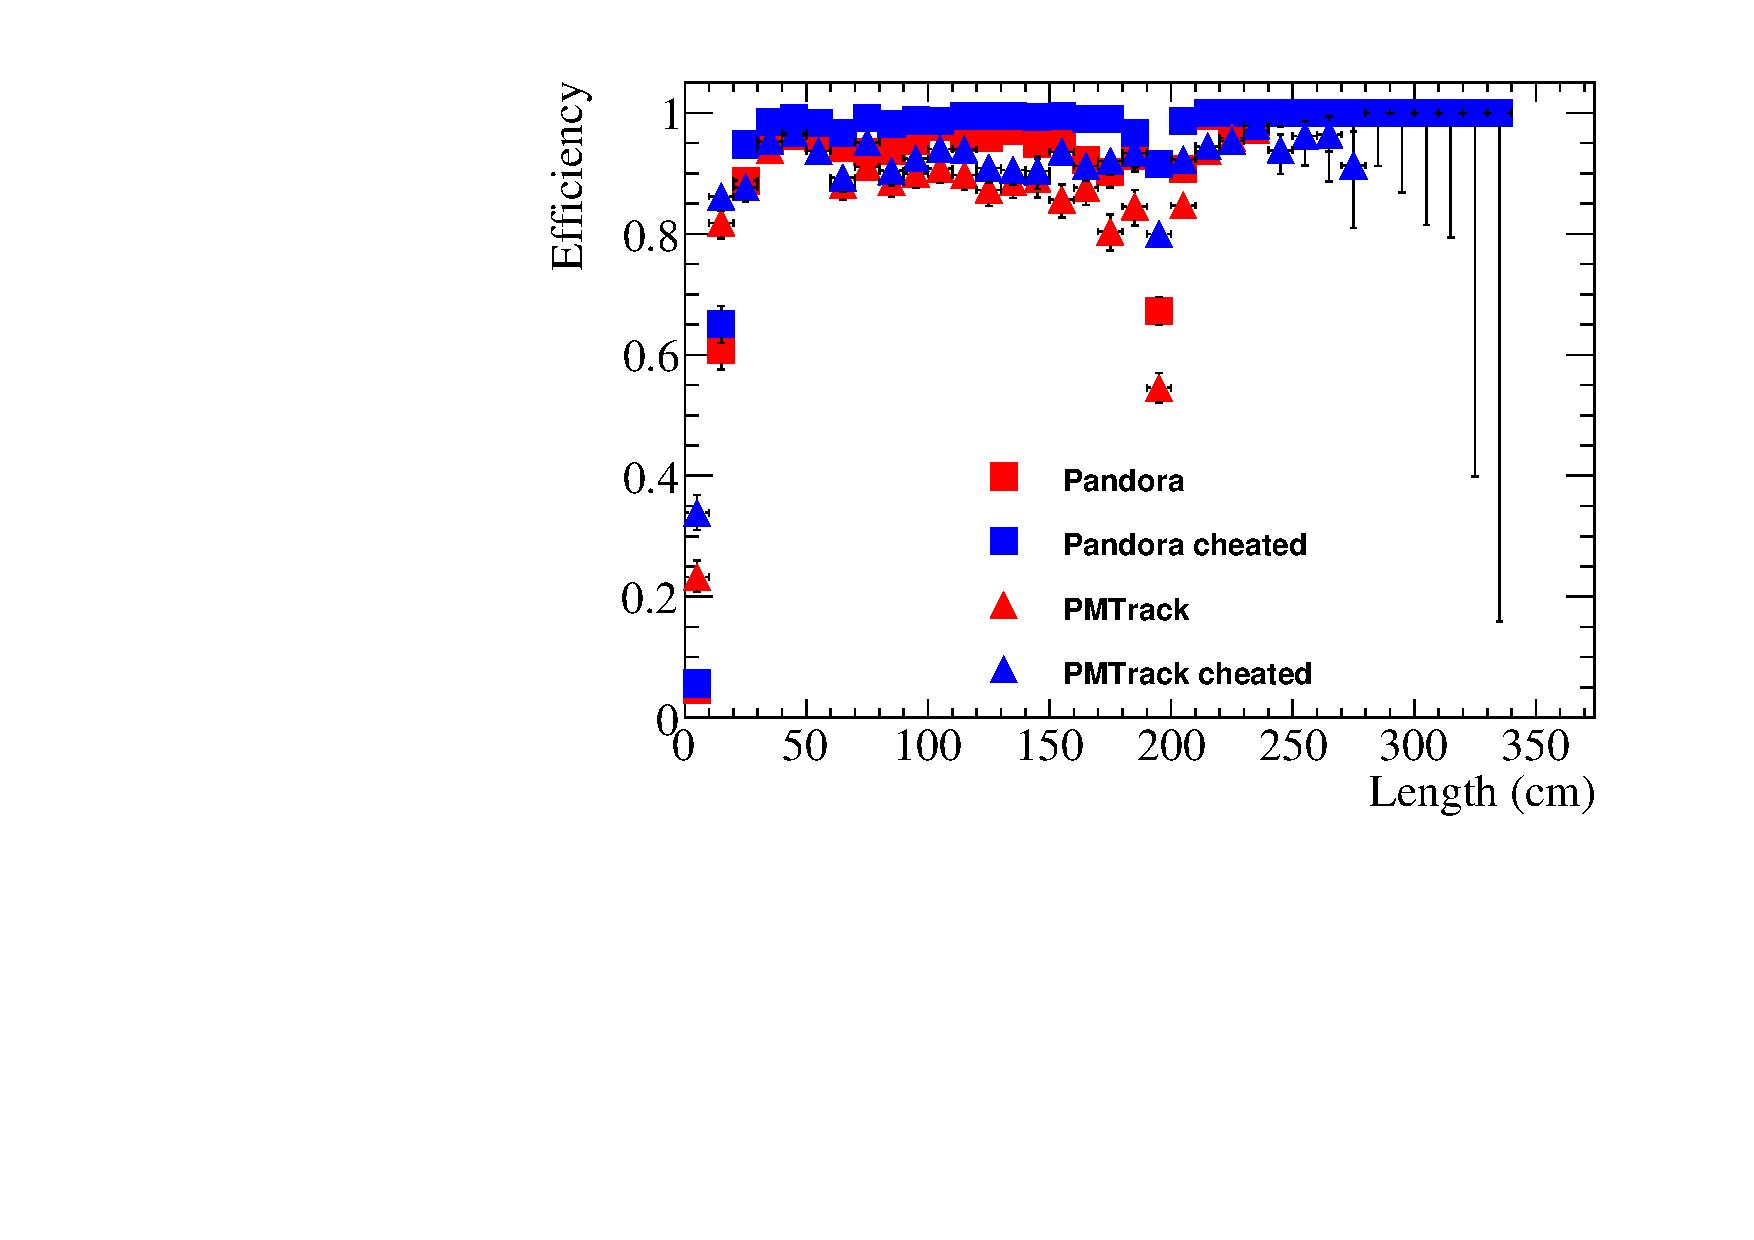
\includegraphics[width=\textwidth]{Effic_AntiMuon_500V_All_Length}
    \caption{Reconstruction efficiencies for an Anti-Muon sample.}
    \label{fig:SimEffic_Length_AMu}
  \end{subfigure}
  \hspace{0.08\textwidth}
  \begin{subfigure}{0.45\textwidth}
    \centering
    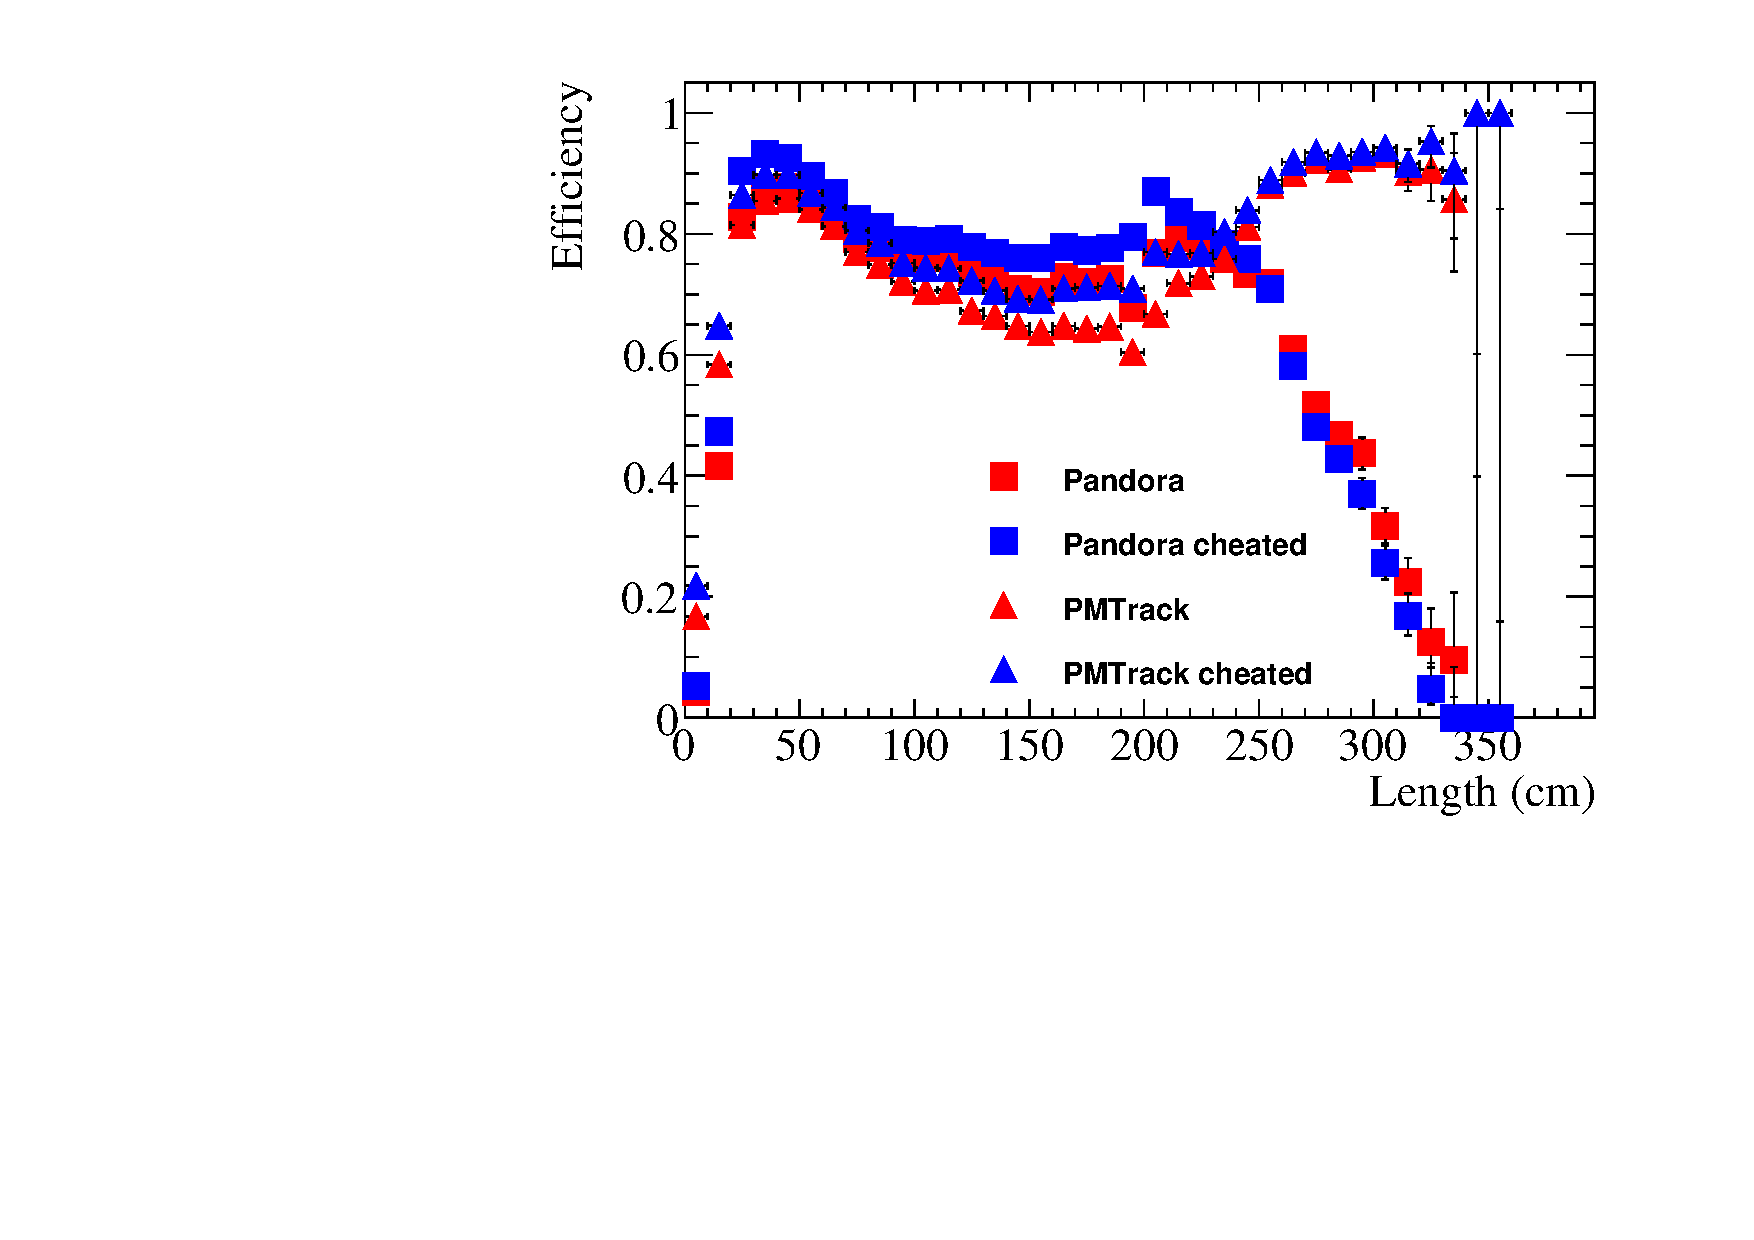
\includegraphics[width=\textwidth]{Effic_Cosmics_500V_All_Length}
    \caption{Reconstruction efficiencies for a CRY sample.}
    \label{fig:SimEffic_Length_CRY}
  \end{subfigure}
  \caption[The reconstruction efficiencies for simulated events as a function of Monte Carlo truth track length.]
          {The reconstruction efficiencies for simulated events as a function of Monte Carlo truth track length. The efficiencies are shown for non-cheated reconstruction (square blocks) and cheated reconstruction (triangle blocks) for both PMTrack (black) and Pandora (blue).}
          \label{fig:SimEffic_Length}
\end{figure}

\begin{figure}[h!]
  \centering
  \begin{subfigure}{0.45\textwidth}
    \centering
    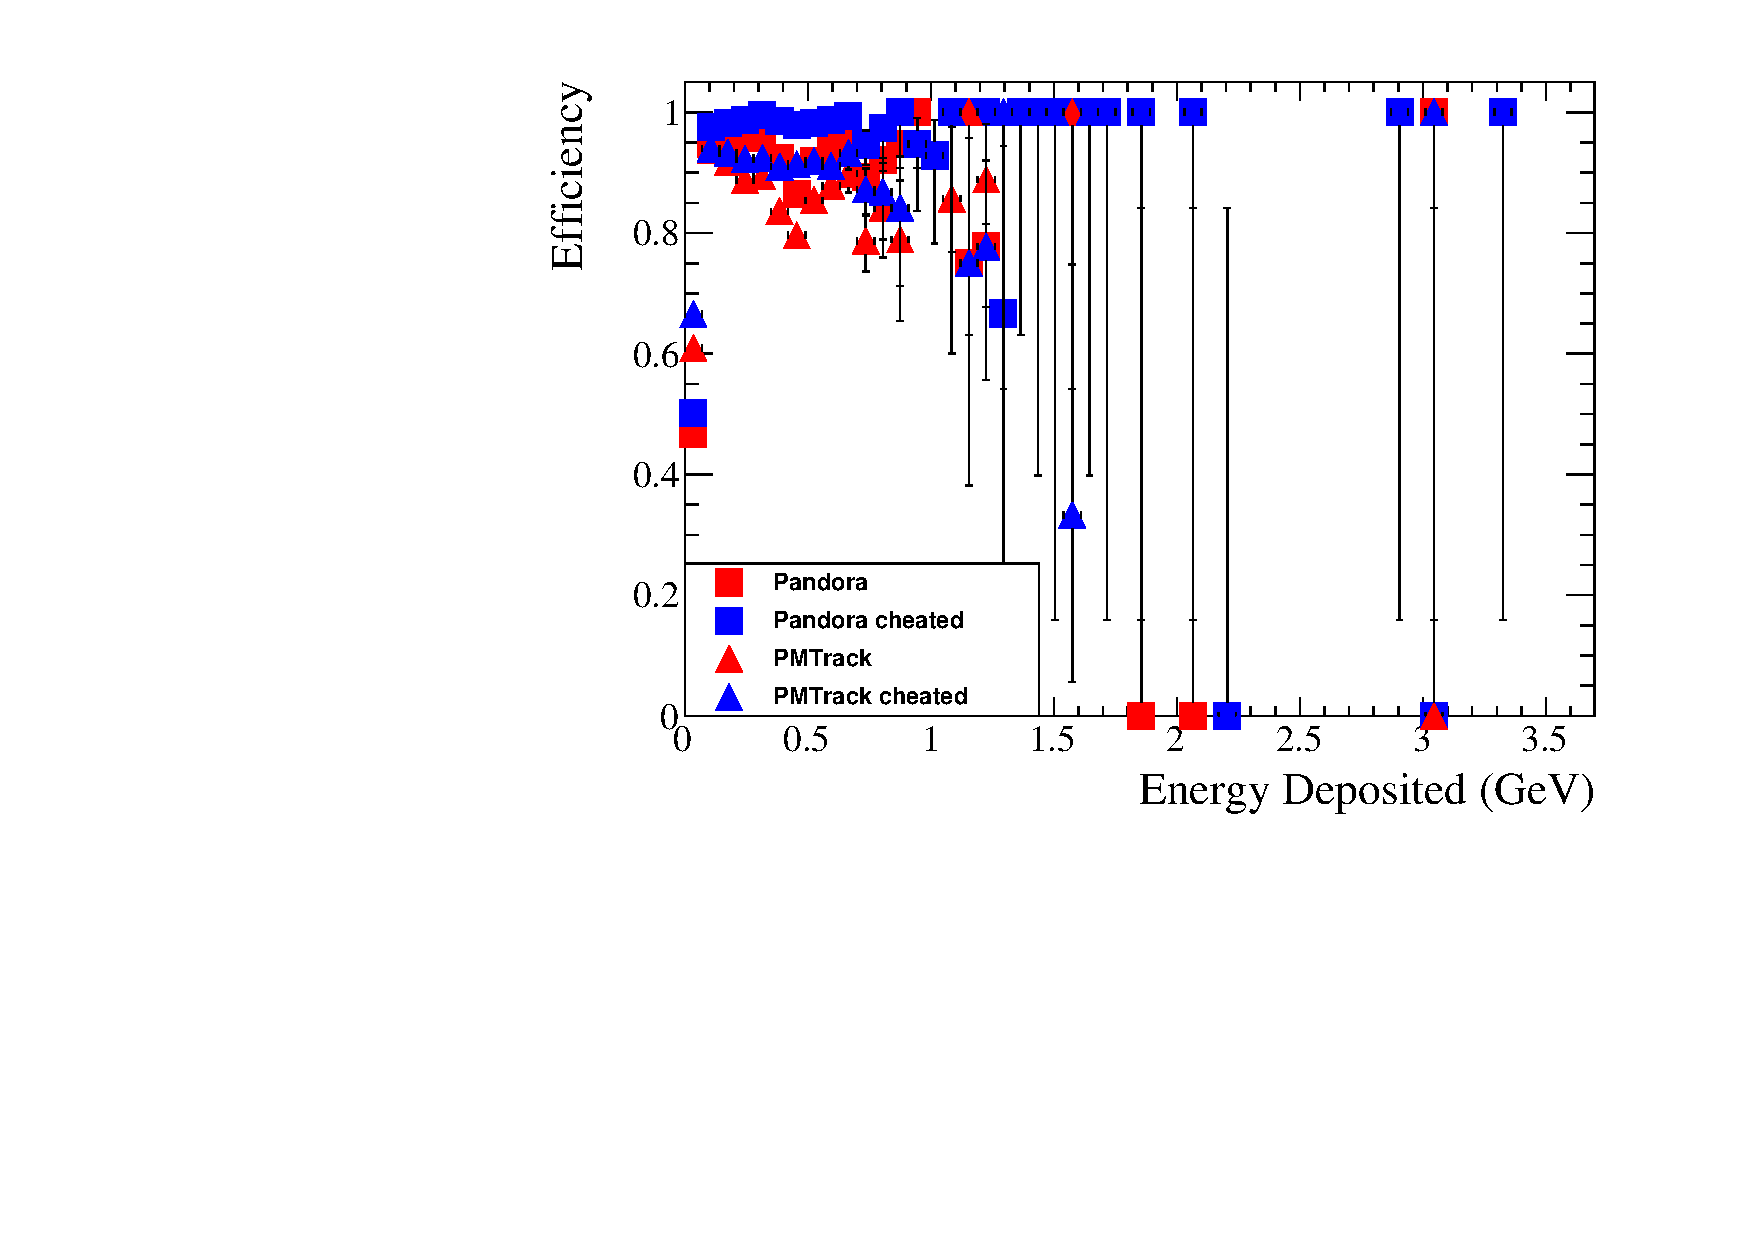
\includegraphics[width=\textwidth]{Effic_AntiMuon_500V_All_EnDepos}
    \caption{Reconstruction efficiencies for an Anti-Muon sample.}
    \label{fig:SimEffic_EnDepos_AMu}
  \end{subfigure}
  \hspace{0.08\textwidth}
  \begin{subfigure}{0.45\textwidth}
    \centering
    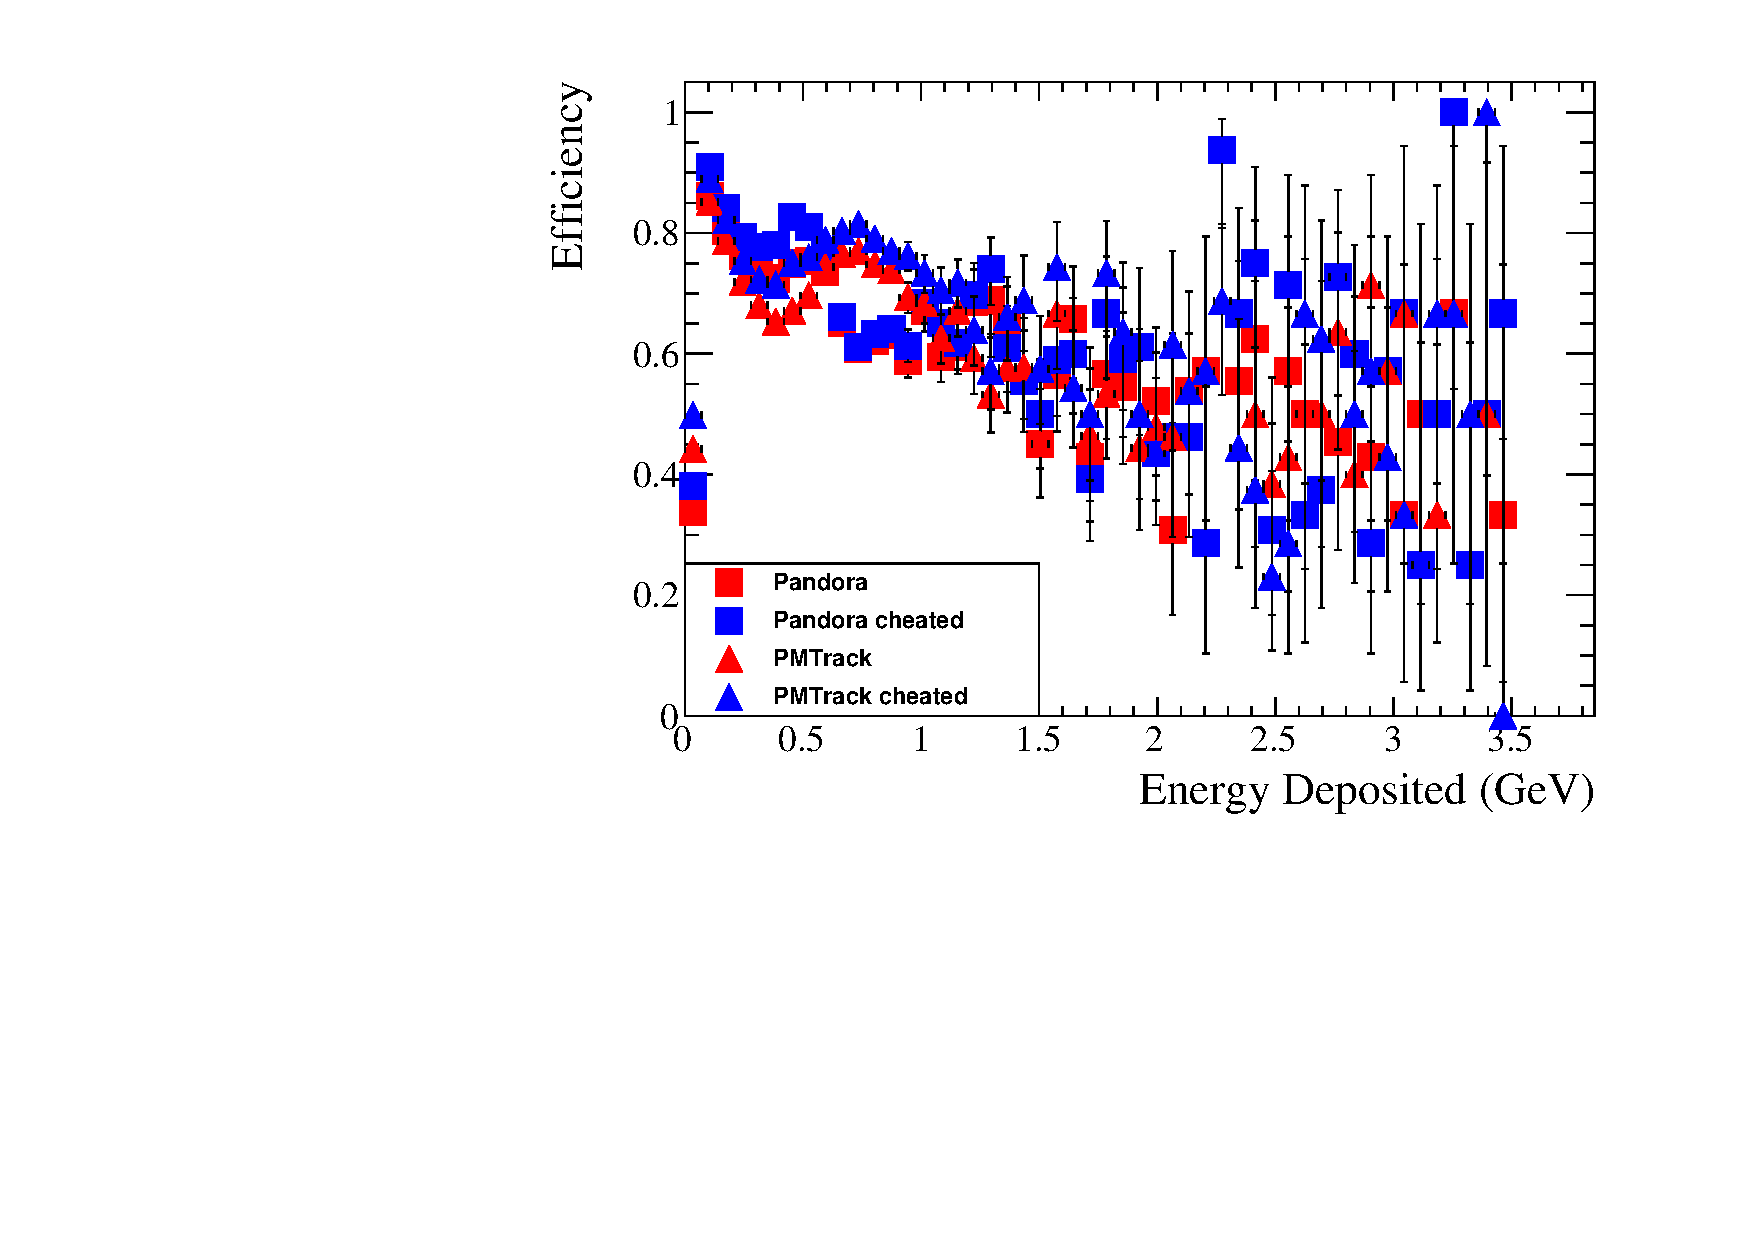
\includegraphics[width=\textwidth]{Effic_Cosmics_500V_All_EnDepos}
    \caption{Reconstruction efficiencies for a CRY sample.}
    \label{fig:SimEffic_EnDepos_CRY}
  \end{subfigure}
  \caption[The reconstruction efficiencies for simulated events as a function of Monte Carlo truth deposited energy.]
          {The reconstruction efficiencies for simulated events as a function of Monte Carlo truth deposited energy. The efficiencies are shown for non-cheated reconstruction (square blocks) and cheated reconstruction (triangle blocks) for both PMTrack (black) and Pandora (blue).}
          \label{fig:SimEffic_EnDepos}
\end{figure}

\begin{figure}[h!]
  \centering
  \begin{subfigure}{0.45\textwidth}
    \centering
    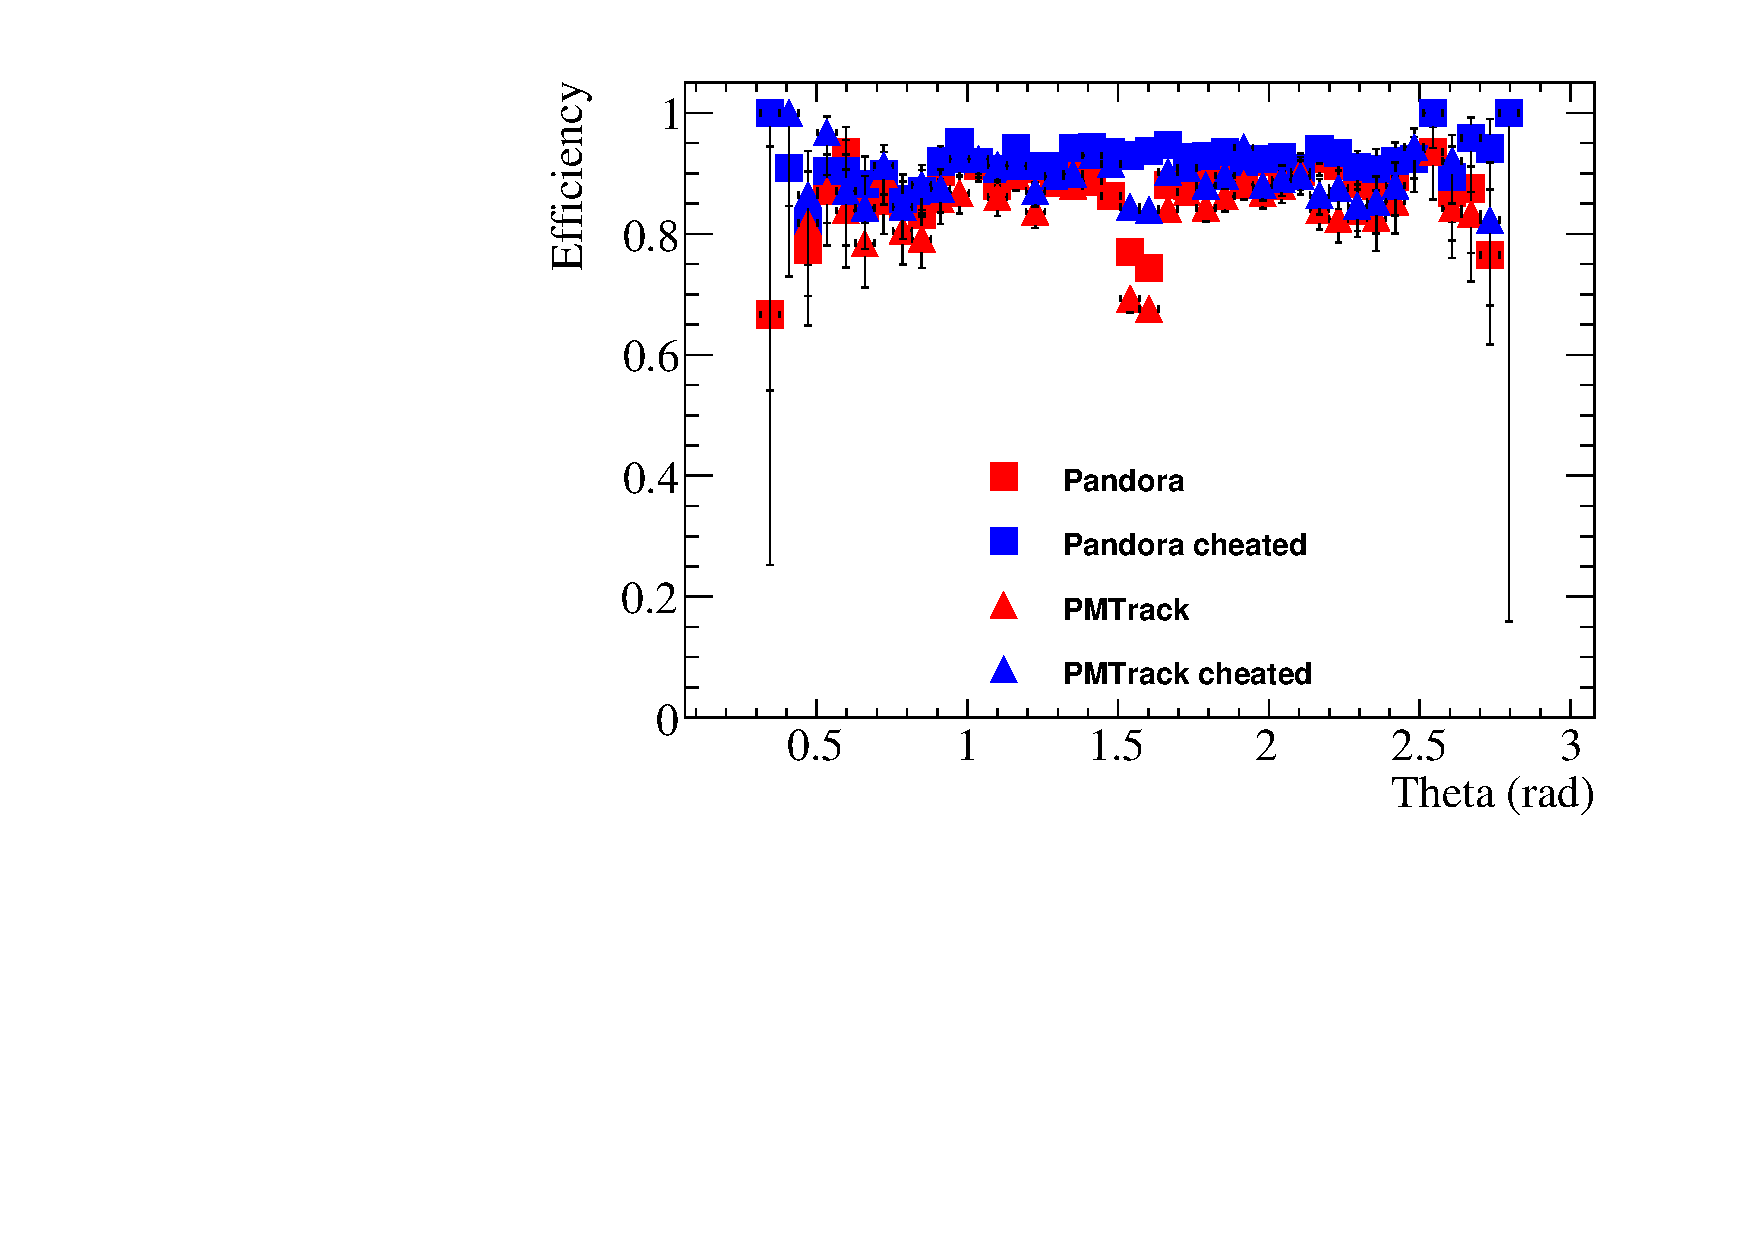
\includegraphics[width=\textwidth]{Effic_AntiMuon_500V_All_Theta}
    \caption{Reconstruction efficiencies for an Anti-Muon sample.}
    \label{fig:SimEffic_Theta_AMu}
  \end{subfigure}
  \hspace{0.08\textwidth}
  \begin{subfigure}{0.45\textwidth}
    \centering
    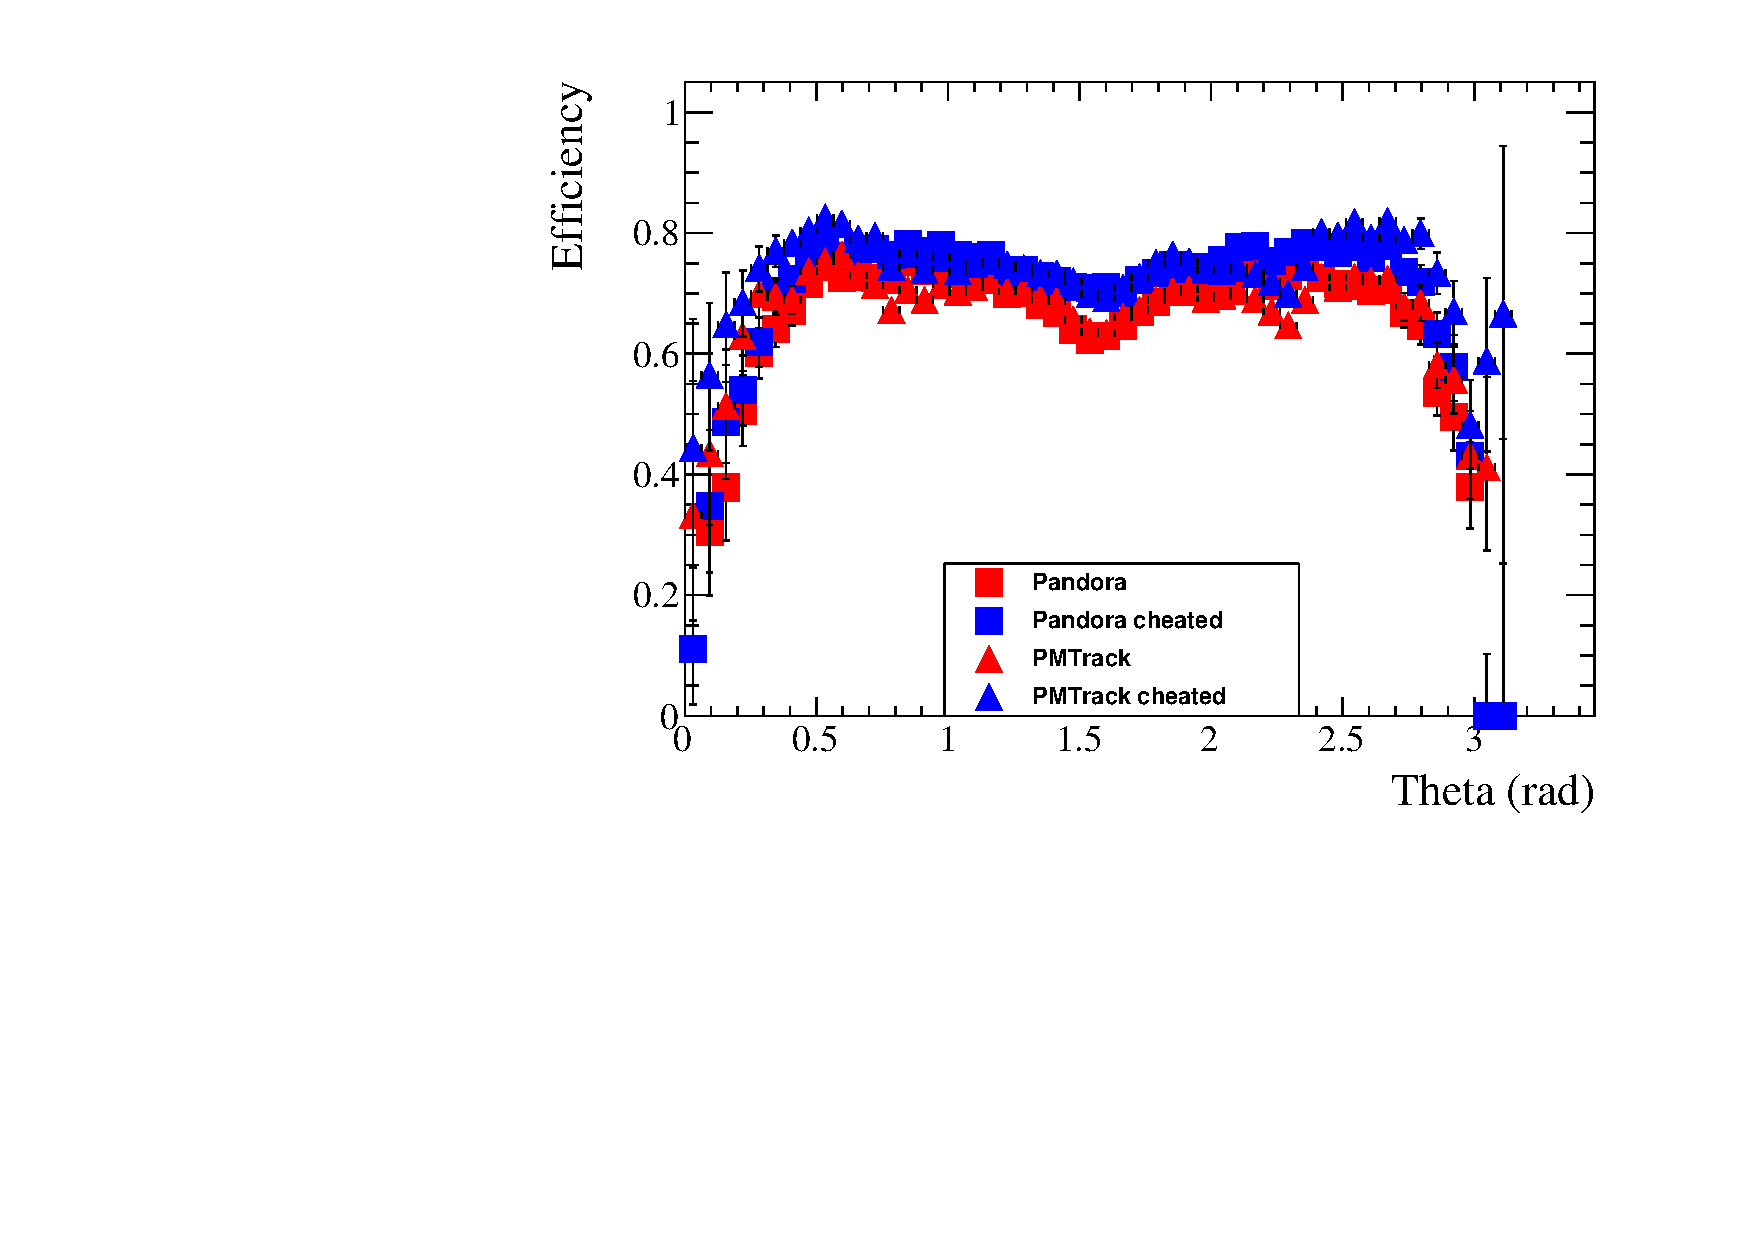
\includegraphics[width=\textwidth]{Effic_Cosmics_500V_All_Theta}
    \caption{Reconstruction efficiencies for a CRY sample.}
    \label{fig:SimEffic_Theta_CRY}
  \end{subfigure}
  \caption[The reconstruction efficiencies for simulated events as a function of Monte Carlo truth track angle in theta.]
          {The reconstruction efficiencies for simulated events as a function of Monte Carlo truth track angle in theta. The efficiencies are shown for non-cheated reconstruction (square blocks) and cheated reconstruction (triangle blocks) for both PMTrack (black) and Pandora (blue).}
          \label{fig:SimEffic_Theta}
\end{figure}

\begin{figure}[h!]
  \centering
  \begin{subfigure}{0.45\textwidth}
    \centering
    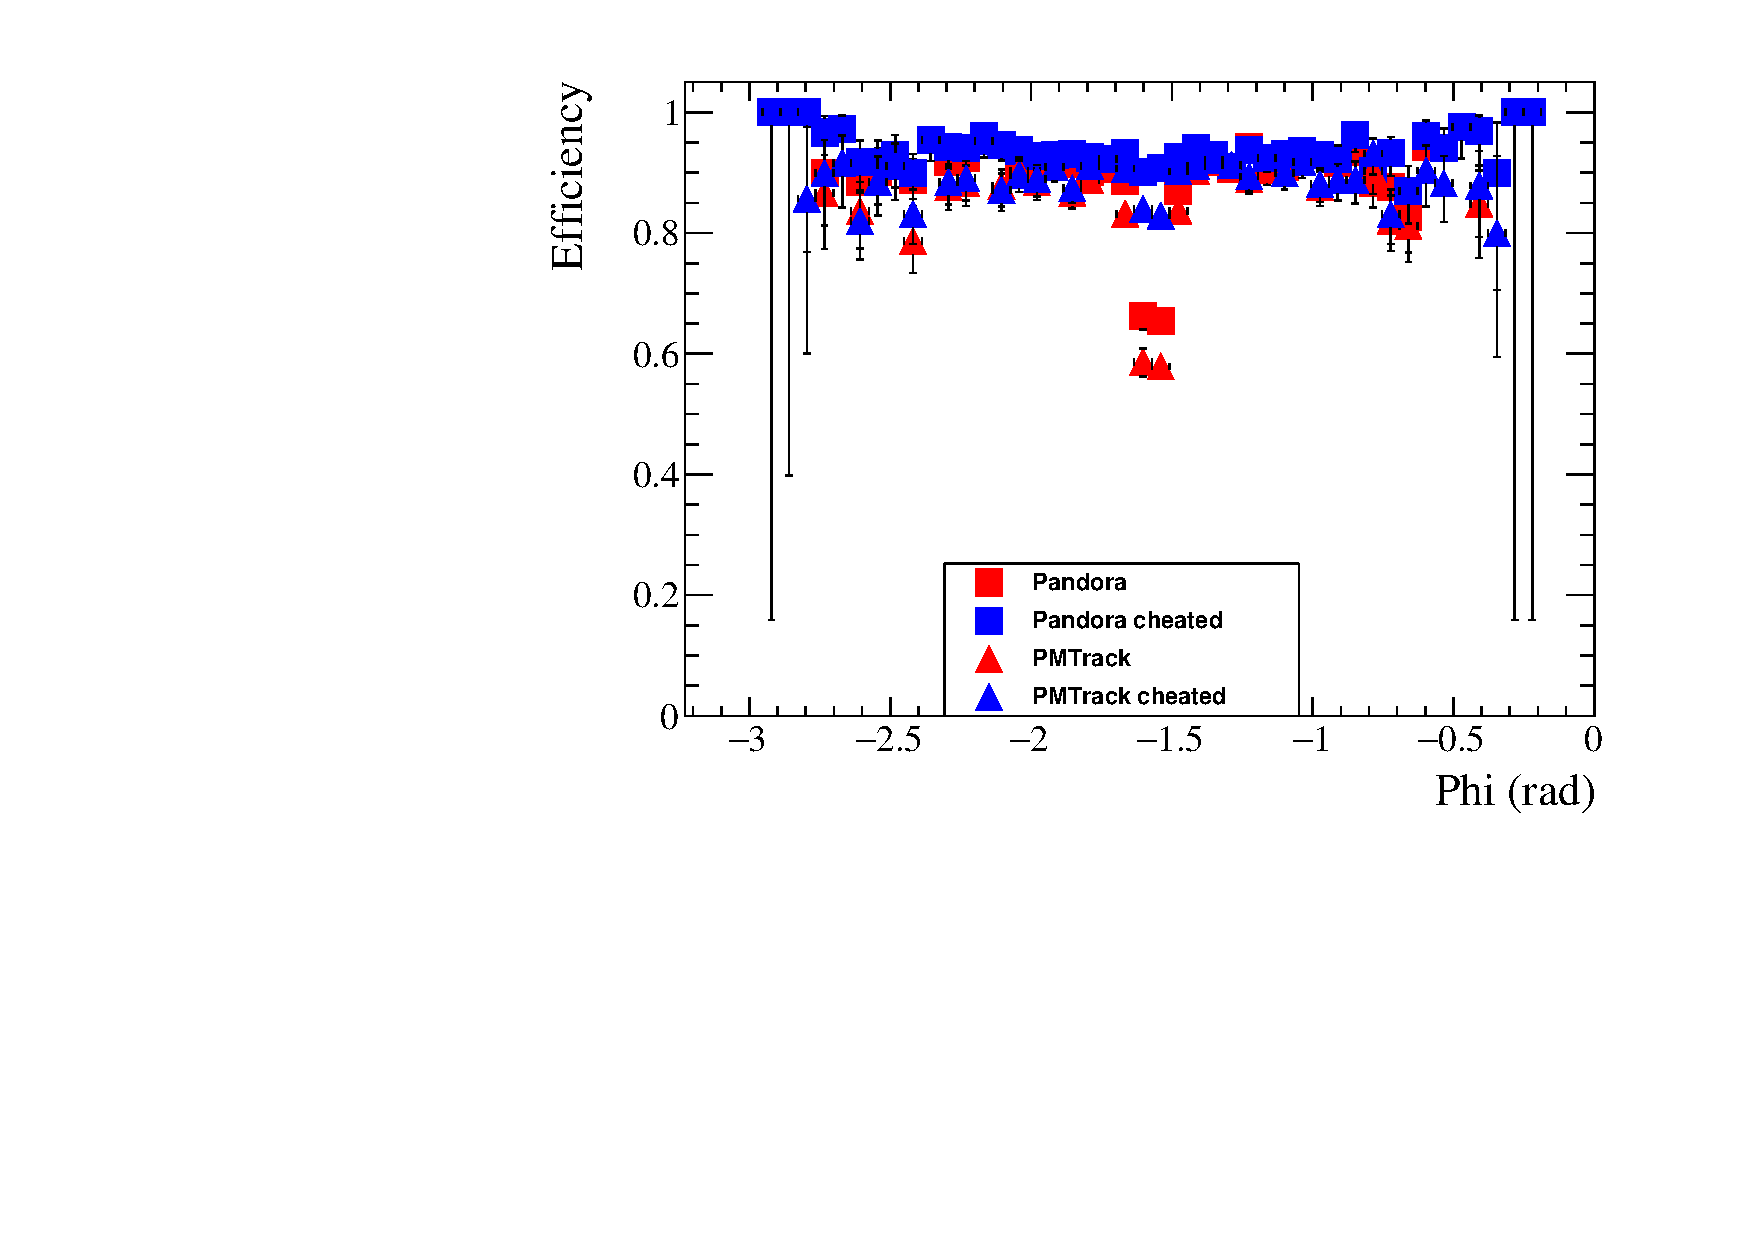
\includegraphics[width=\textwidth]{Effic_AntiMuon_500V_All_Phi}
    \caption{Reconstruction efficiencies for an Anti-Muon sample.}
    \label{fig:SimEffic_Phi_AMu}
  \end{subfigure}
  \hspace{0.08\textwidth}
  \begin{subfigure}{0.45\textwidth}
    \centering
    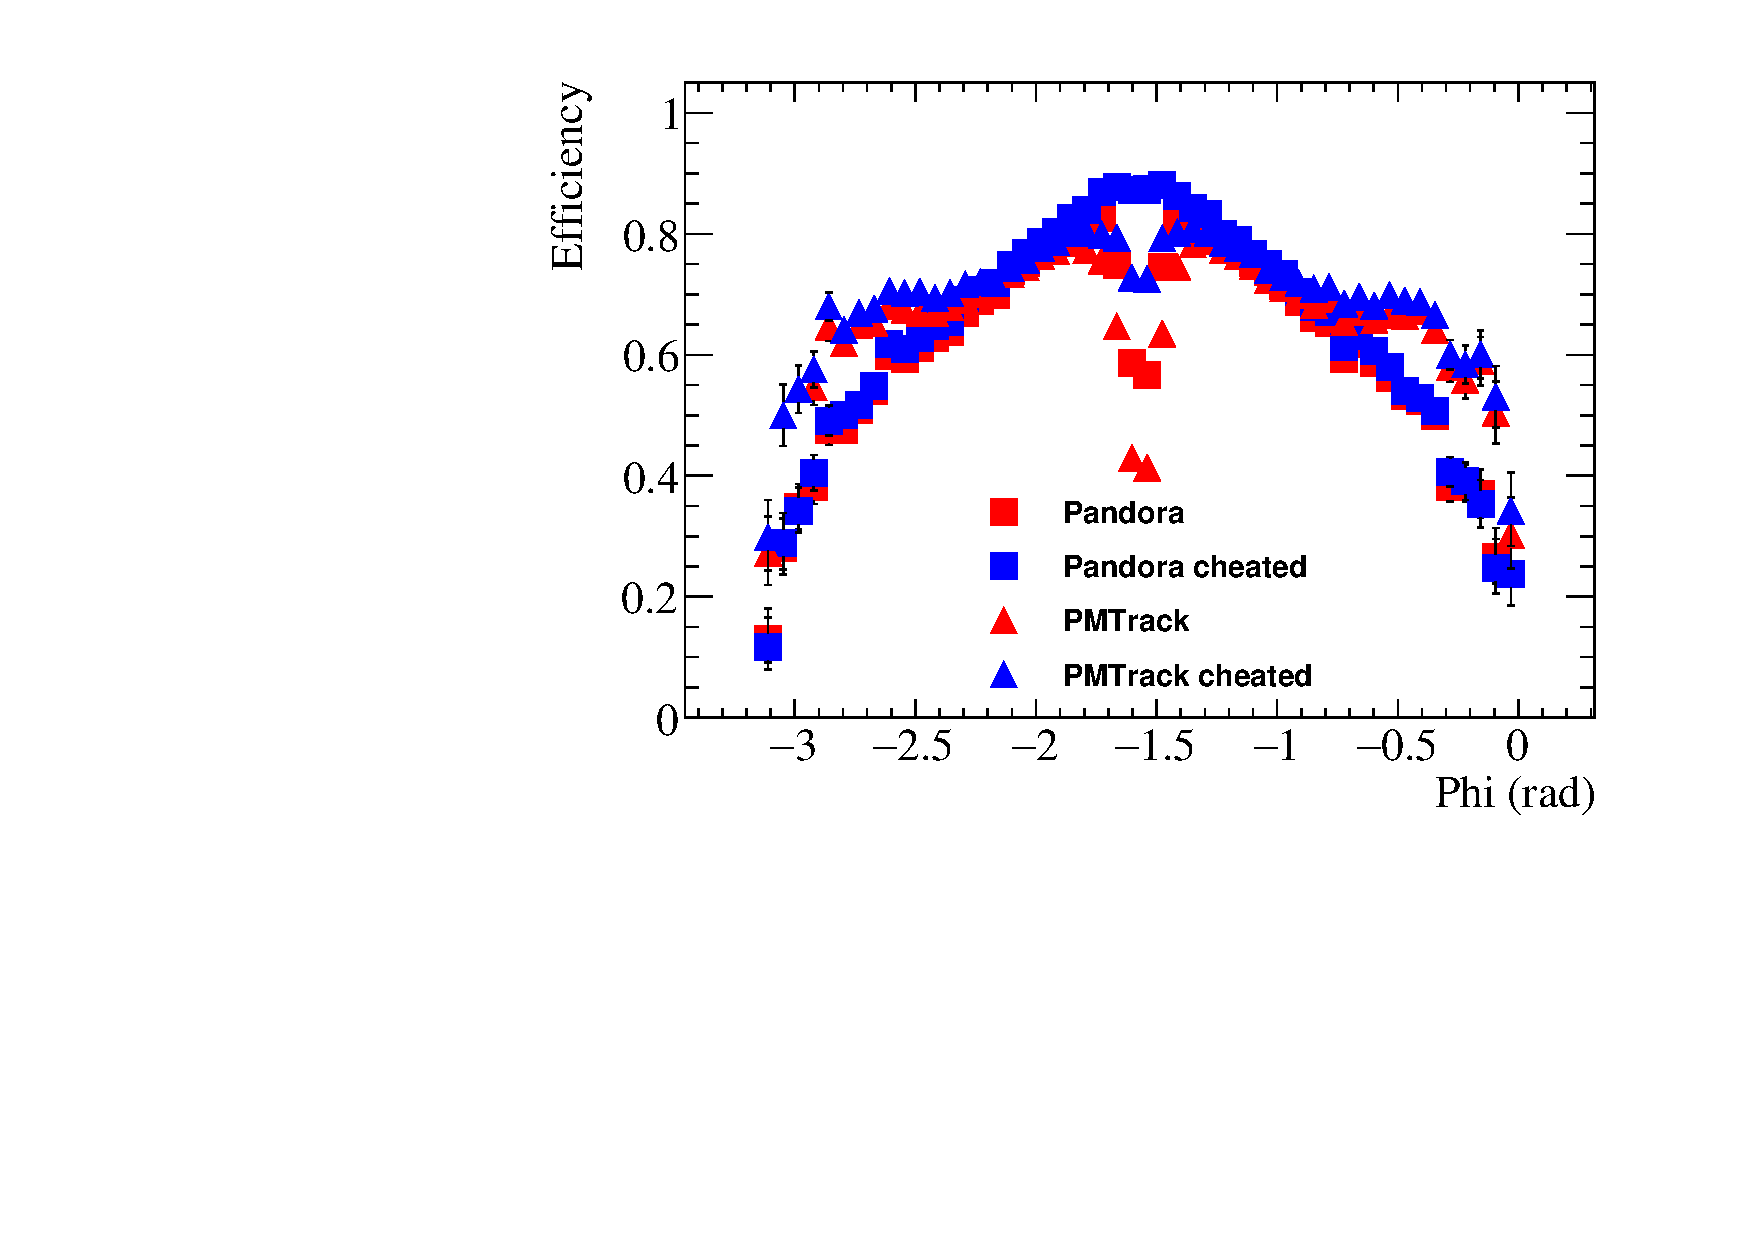
\includegraphics[width=\textwidth]{Effic_Cosmics_500V_All_Phi}
    \caption{Reconstruction efficiencies for a CRY sample.}
    \label{fig:SimEffic_Phi_CRY}
  \end{subfigure}
  \caption[The reconstruction efficiencies for simulated events as a function of Monte Carlo truth track angle in phi.]
          {The reconstruction efficiencies for simulated events as a function of Monte Carlo truth track angle in phi. The efficiencies are shown for non-cheated reconstruction (square blocks) and cheated reconstruction (triangle blocks) for both PMTrack (black) and Pandora (blue).}
          \label{fig:SimEffic_Phi}
\end{figure}

\begin{figure}[h!]
  \centering
  \begin{subfigure}{0.45\textwidth}
    \centering
    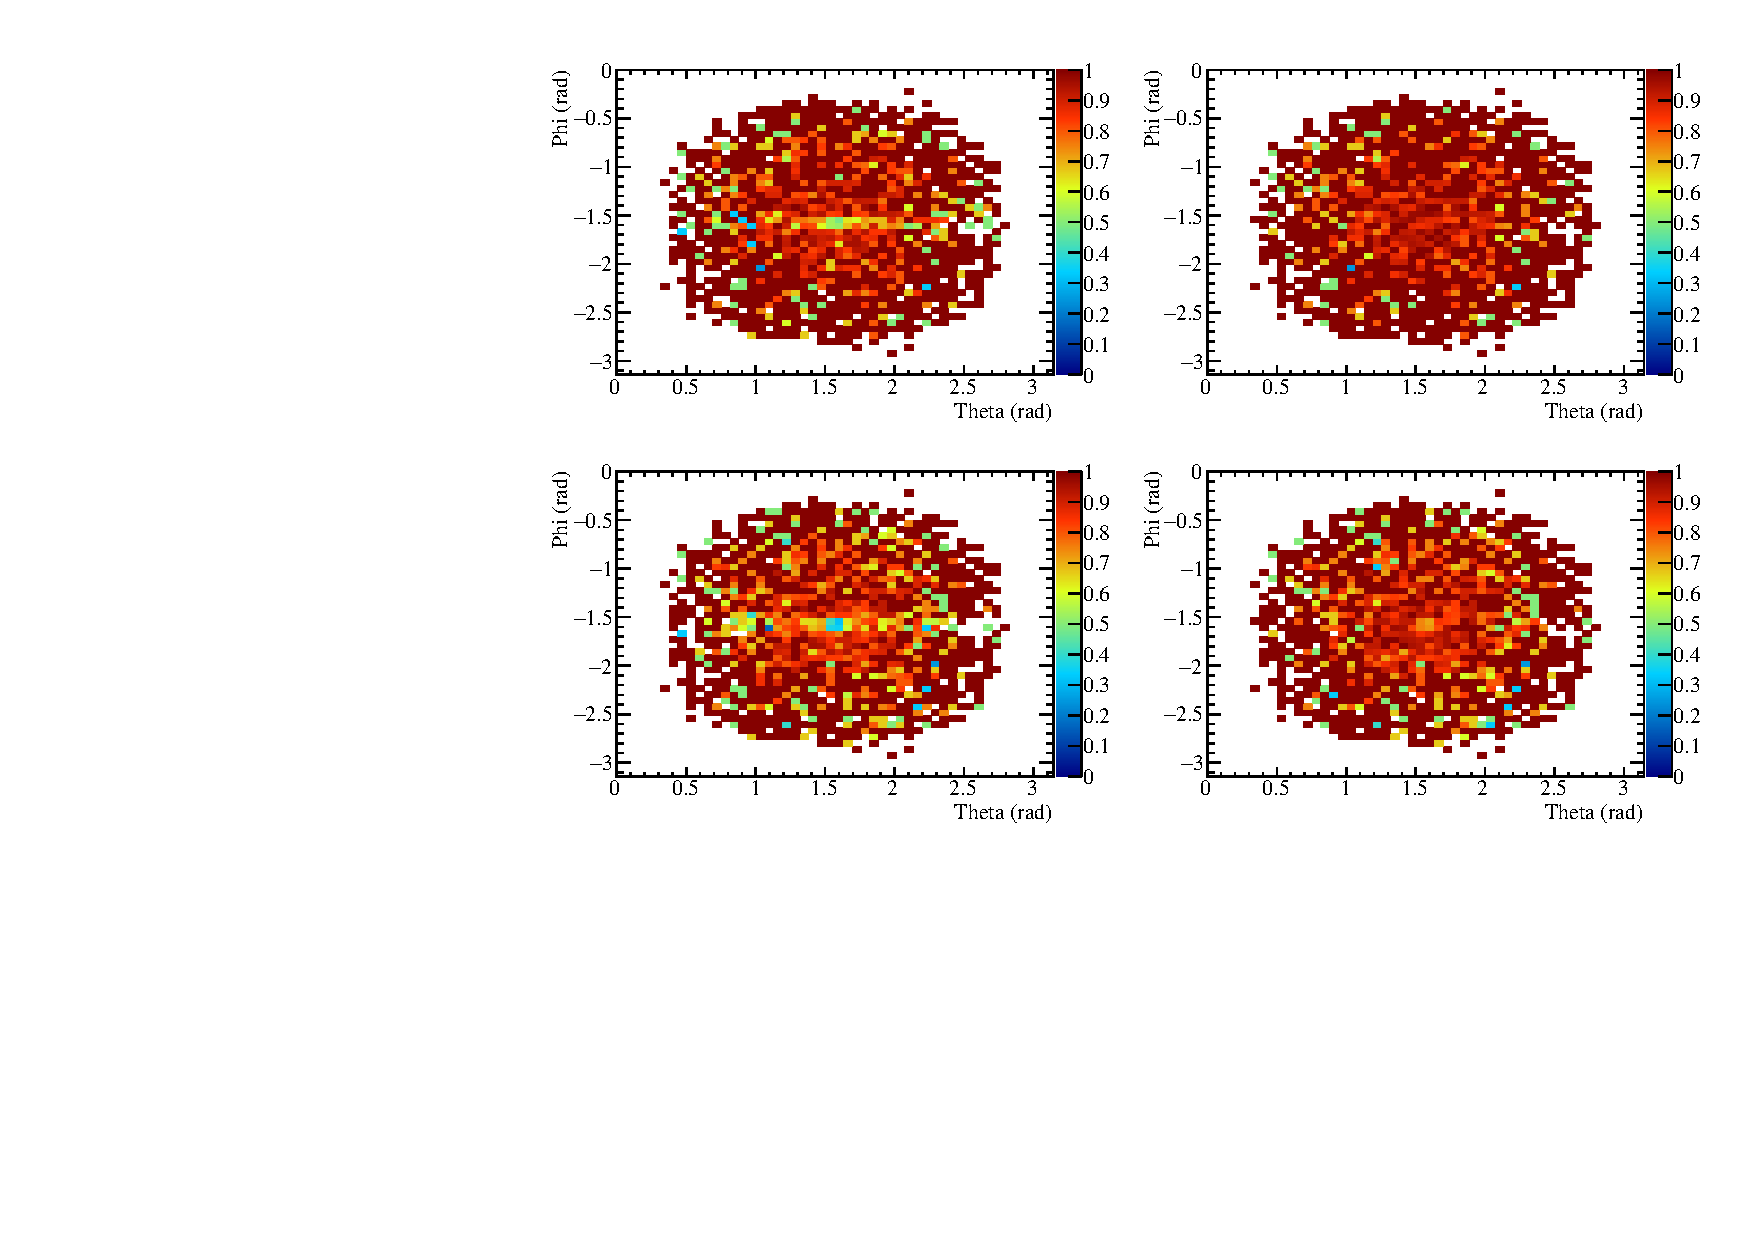
\includegraphics[width=\textwidth]{Effic_AntiMuon_500V_All_PhiTheta}
    \caption{Reconstruction efficiencies for an Anti-Muon sample.}
    \label{fig:SimEffic_ThetaPhi_AMu}
  \end{subfigure}
  \hspace{0.08\textwidth}
  \begin{subfigure}{0.45\textwidth}
    \centering
    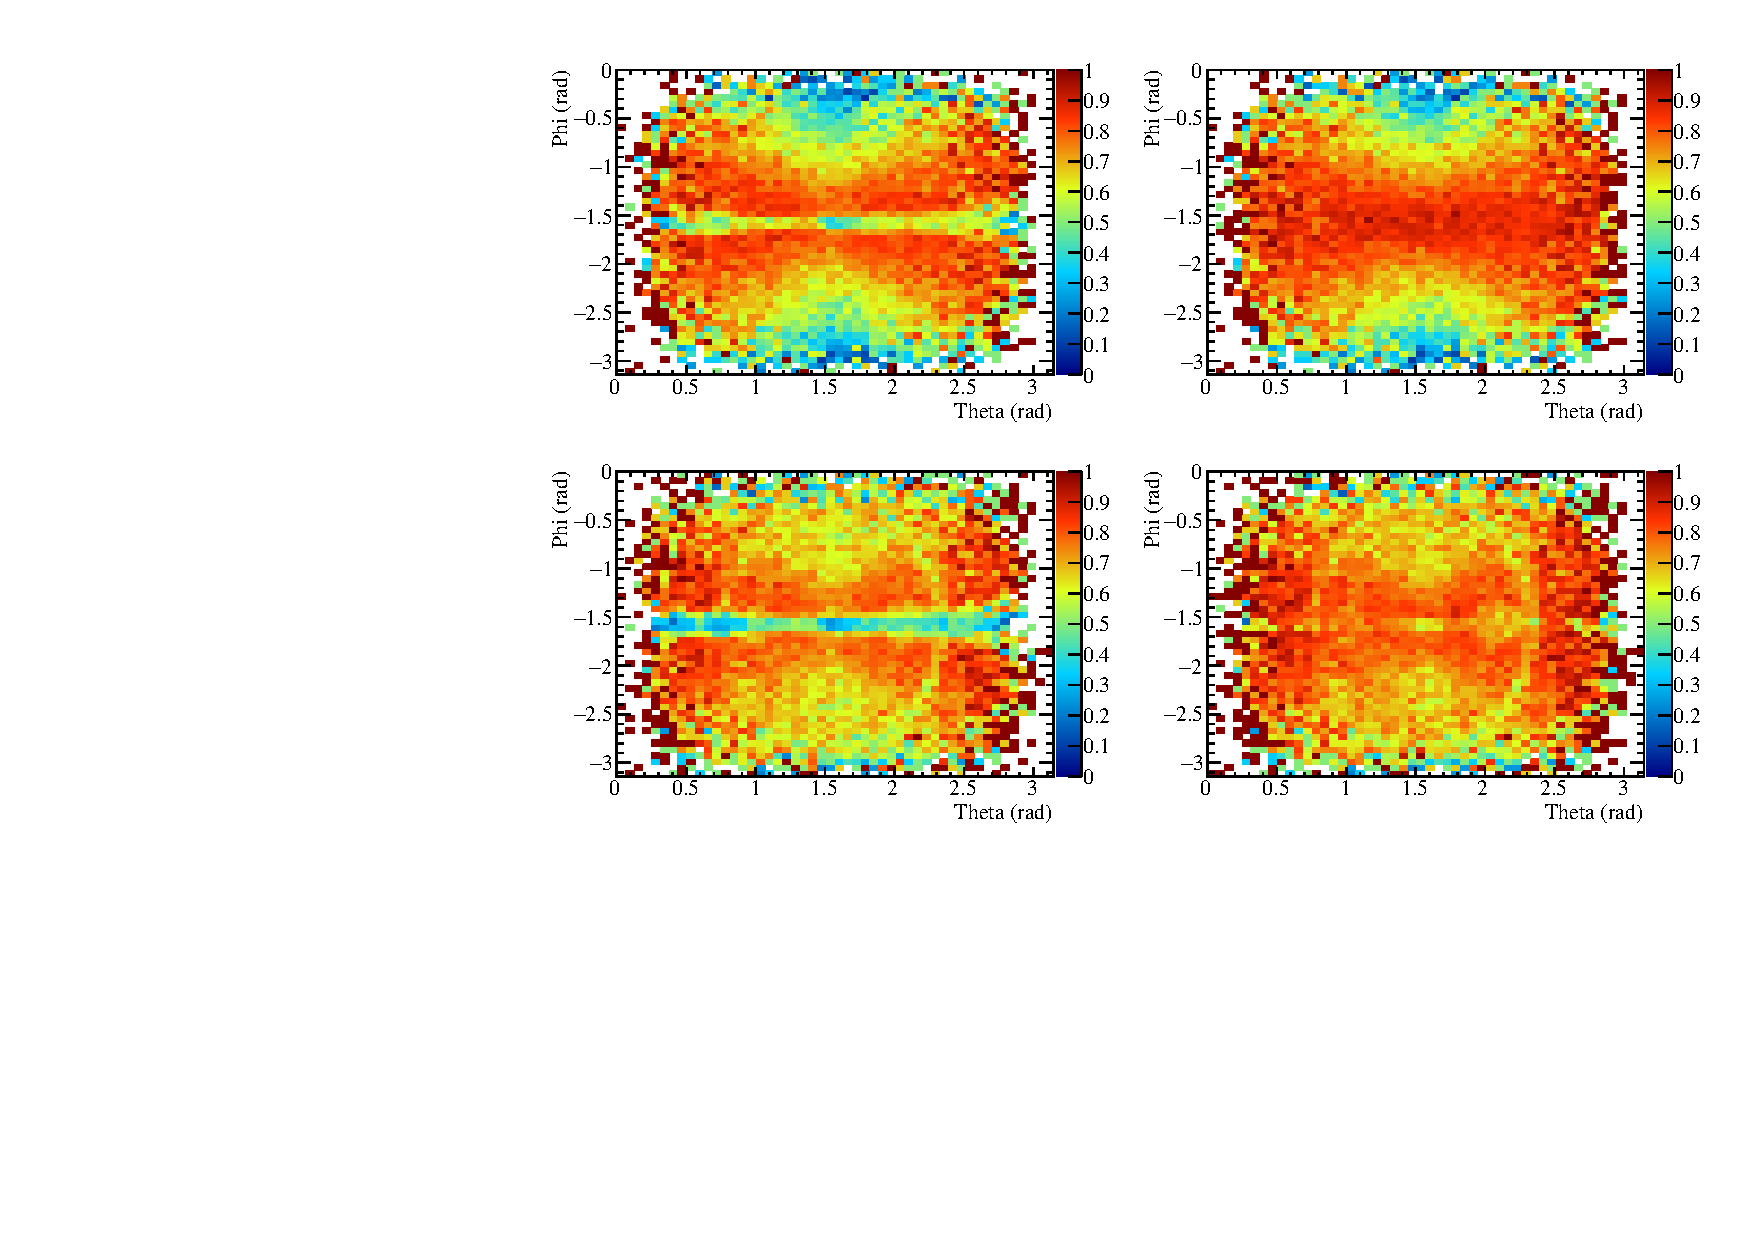
\includegraphics[width=\textwidth]{Effic_Cosmics_500V_All_PhiTheta}
    \caption{Reconstruction efficiencies for a CRY sample.}
    \label{fig:SimEffic_ThetaPhi_CRY}
  \end{subfigure}
  \caption[The reconstruction efficiencies for simulated events as a function of Monte Carlo truth track angle in theta and phi.]
          {The reconstruction efficiencies for simulated events as a function of Monte Carlo truth track angle in theta and phi. The efficiencies are shown for non-cheated reconstruction (plots on the left) and cheated reconstruction (plots on the right) for both Pandora (plots on the top) and PMTrack (plots on the bottom).}
          \label{fig:SimEffic_ThetaPhi}
\end{figure}

A striking feature of Figure~\ref{fig:SimEffic_Length} is the rapid decrease in reconstructed efficiency for the CRY sample for track lengths above 250 cm when using Pandora. The cause of this is that tracks are reconstructed separately in the long and short drift volumes before being merged when they are found to be co-linear in the $yz$ plane. This is not a problem in the Anti-Muon sample as the $x$ position of the hits calculated using Equation~\ref{eq:HitTime} will be correct. However, when the same is done for hits in the CRY sample using particles with large interaction times the $x$ positions will have offsets proportional to the interaction time unless the hit time is corrected by Equation~\ref{eq:HitTime_Int}. The result of this is that merged tracks can have discontinuities in their $x$ coordinates of more than 20 m. As the interaction time of the track is calculated using the output of the tracking algorithms it is not possible to directly correct for the interaction time at present. It is however possible to subtract this jump in $x$ position from the track length quantity which is calculated when the stitched track is stored in the event, this will give the correct track length though the user will still have to correct individual hit positions in later analyses using the calculated interaction time. This is what is done by PMTrack, hence it not exhibiting this rapid decrease in reconstruction efficiency for long tracks. \\

\begin{subequations} \begin{align}
  x_{Hit} &= T_{Hit} \times v_{Drift} \label{eq:HitTime} \\
  T_{Hit} &= T_{Measured} - T_{Interaction} \label{eq:HitTime_Int}
\end{align} \end{subequations}

It is clear from Figure~\ref{fig:SimEffic_Length} that tracks of lengths less than 30 cm are poorly reconstructed. The very low efficiency for tracks of less than 10 cm can be partially attributed to particles of lengths less than 1 cm as these particles are too short to be reconstructed using the current reconstruction process. These very short particles represent ~30\% of the particles with lengths below 10 cm. Though these particles will need to be reconstructed when looking for supernovae bursts special algorithms will probably be written as these particles will only cross 1 or 2 wires in each plane and so may look similar to noise hits meaning that they will not be combined into clusters. Another issue is that the low energies of these particles may mean that the hits are below threshold and so will not be reconstructed. The reconstruction of longer tracks will also be affected by the number of wires which they cross, though this should matter much less for particles with lengths of more than 5 cm as they will have crossed roughly 10 wires in each plane, this should be enough to reliably construct clusters. This can be seen to be the case for PMTrack when considering the Anti-Muon sample, as the efficiencies for track lengths between 10 and 20 cm is roughly the same as that for track lengths between 20 and 30 cm, however when considering the CRY sample there is still a significant decrease in efficiency. This is attributed to the more complex event structure in the CRY sample, where secondary particles are produced which are mis-reconstructed, as when considering only muons the reconstruction efficiency is seen to be the same as that for the Anti-Muon sample. \\

The trend of increasing efficiency for longer track lengths from Figure~\ref{fig:SimEffic_Length} can also be seen in Figure~\ref{fig:SimEffic_EnDepos} as the energy deposited increases. This is because particles which deposit more energy will tend to have travel further in the detector. The amount of energy that particles deposit is limited by the size of the detector though as particles with an energy of more than 1 GeV are energetic enough to through-going MIPS. This results in few particles depositing more than 1 GeV in the detector causing the uncertainty in the reconstruction efficiency to increase above this energy. \\

It is also interesting to note the pronounced decreases in reconstruction efficiencies for particular angles shown in Figure~\ref{fig:SimEffic_Theta} and Figure~\ref{fig:SimEffic_Phi}. The decrease in efficiency at $\phi = \frac{\pi}{2}$ can be attributed to the drop in efficiency for tracks of ~200 cm, as this corresponds to the vertical height of the detector meaning that few collection wires are hit and so determining the triple points needed by the disambiguation are difficult to find. This is verified by the large increase in efficiency achieved by cheating the disambiguation. Similarly the decrease in efficiency at $\theta = \frac{\pi}{2}$ can be attributed to particles which are perpendicular to the collection wires resulting in few collection wires being hit. \\  

The information from Figures~\ref{fig:SimEffic_Theta} and~\ref{fig:SimEffic_Phi} is combined in Figure~\ref{fig:SimEffic_ThetaPhi} where the sharp drops in efficiency for the CRY sample are particularly visible. The effect of cheated disambiguation is clear in Figure~\ref{fig:SimEffic_ThetaPhi_CRY} where the dip in efficiency as a function of $\theta$ at fixed $\phi=\frac{\pi}{2}$ is completely removed. The same is not true for the dip in efficiency as a function $\phi$ at fixed $\theta = \frac{\pi}{2}$, though the reduction in efficiency was not uniform or as severe across all values of $\theta$ as it remains mainly confined to values of $\theta$ close to 0 or $\pi$, particularly when using Pandora . The observation that a significant improvement in the quality of reconstruction can be made in improving the disambiguation is a driving force in the wire pitches being 36$^{\circ}$ for the DUNE FD as opposed 45$\pm$0.7$^{\circ}$ in the 35 ton, because as discussed in Section~\ref{sec:LArSoft} the shallower wire pitch makes disambiguation easier. Though disambiguation will be easier in the different geometry, further efforts to improve disambiguation are still required, as are continued efforts to reconstruct the shortest tracks. \\

%********************************** % Fourth Section  *************************************
\section{Performing particle identification}  \label{sec:PID} %Section - X.4
Being able to perform reliable particle identification (PID) is key deliverable for the DUNE experiment, and so efforts have been made to establish a metric by which this can be achieved. The predominant method of performing PID in LAr is to use the relationship between $\frac{dE}{dx}$ and the residual range of the track, defined as being the distance between a point on the track and the stopping point of the track. The relationship between these particle is observed to be dependent on particle mass and is quantified by the Bethe-Bloch equation!!!citep{BetheBloch}!!! which is shown in Figure~\ref{fig:BetheBloch}. The sharp increase in energy loss per unit length can be seen to occur at different momenta for different particle masses meaning that the peak value of $\frac{dE}{dx}$ can change significantly. One example of a large change in the peak value of $\frac{dE}{dx}$ can be seen by comparing muons and protons, whist muons and pions are very similar. \\

\begin{figure}[h!]
  \centering
  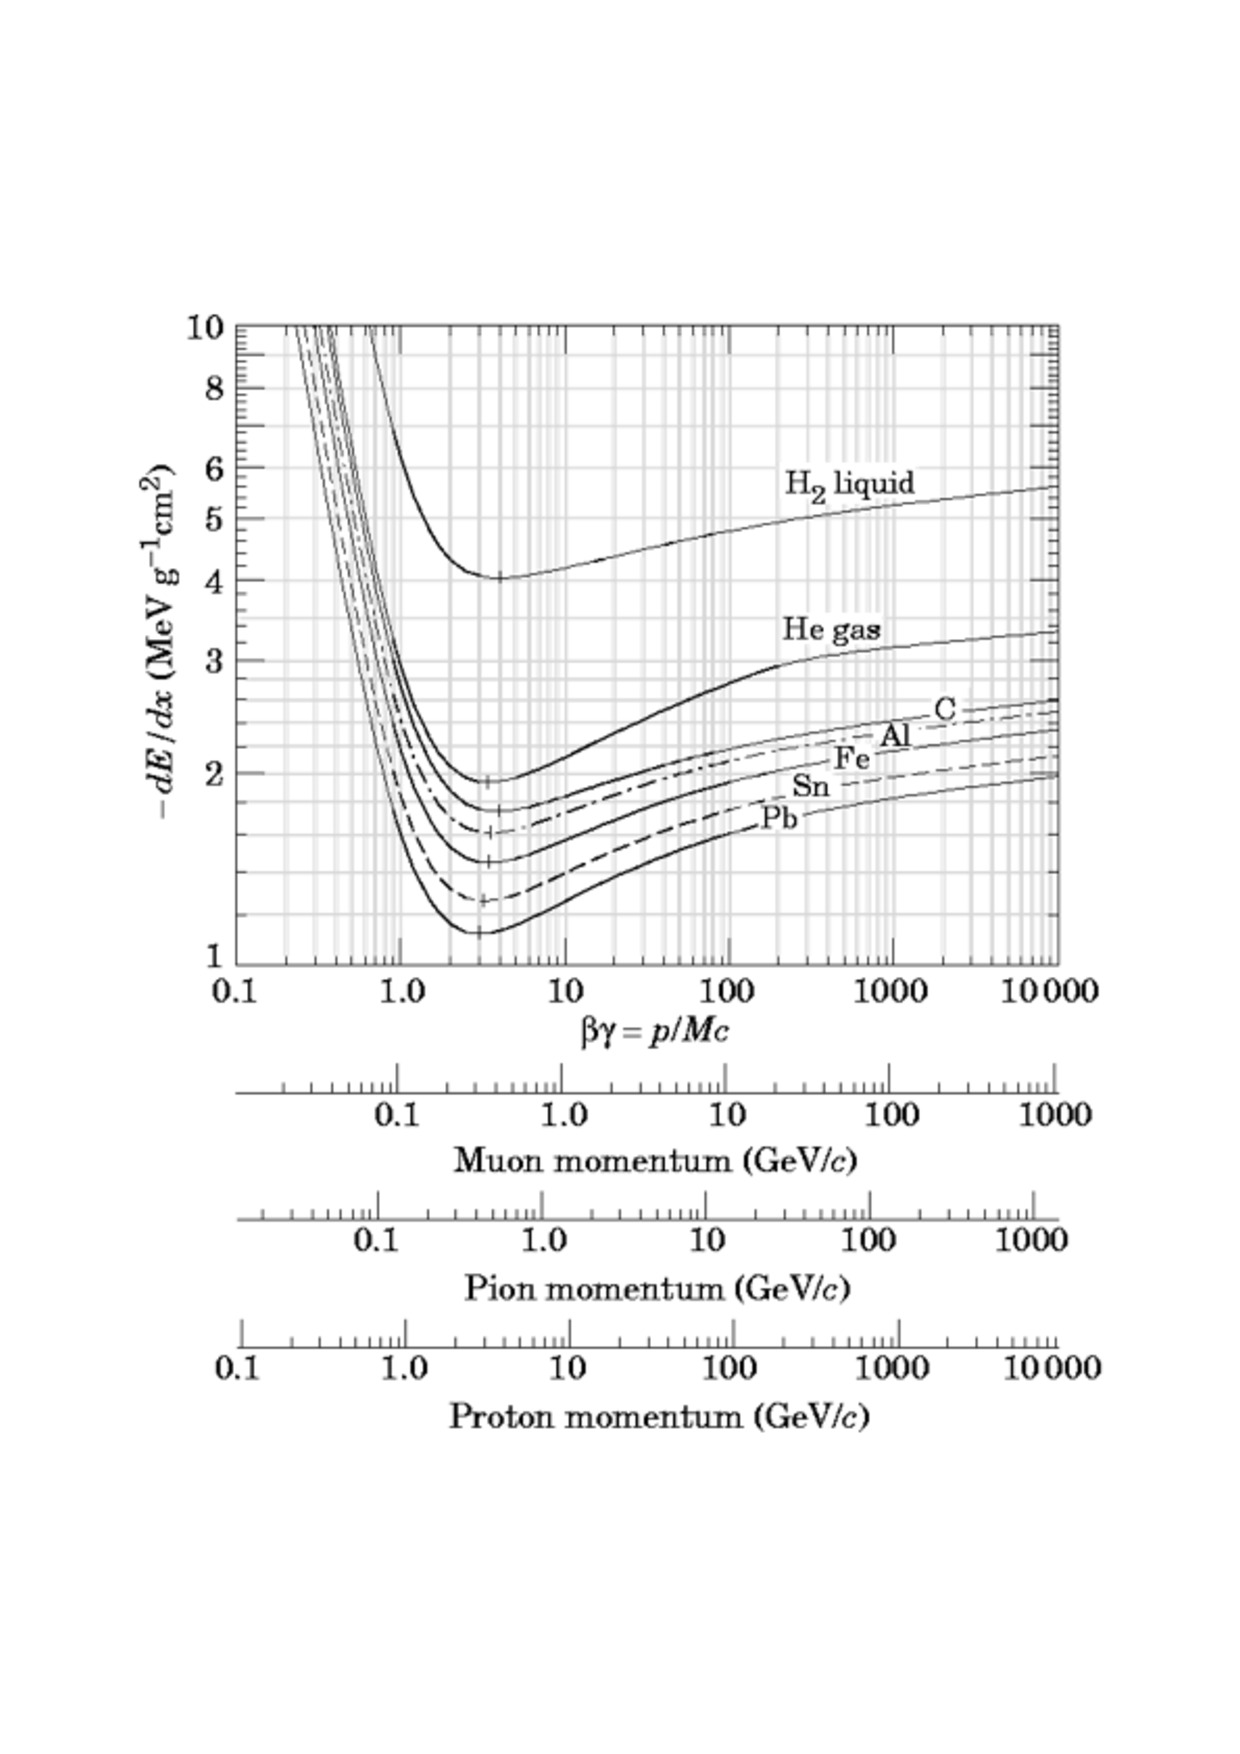
\includegraphics[width=0.5\textwidth]{BetheBlock}
  \caption[The medium and particle type dependence of the Bethe-Bloch equation]
          {The Bethe-Bloch equation describes energy loss per unit length as a function of energy in different mediums. The energy losses expected for different particle types is shown in different mediums. Liquid Argon with a density of 1.4 g cm$^{-3}$ has a density slightly less than that of Carbon at 1.8 g cm$^{-3}$.}
  \label{fig:BetheBloch}
\end{figure}

The particle mass dependence can be seen by plotting the $\frac{dE}{dx}$ against the residual range of the particle on a log-log plot, as shown in Figure~\ref{fig:PIDA_loglog}. A power law dependence is found to describe the relationship~\citep{PIDA_Paper}, as shown in Equation~\ref{eq:PIDA}. The dependence on $b$ is found to be weak, and so can be set to -0.42 for all particle masses. This means that the main discriminant used is the $A$ parameter, which has a strong dependence on particle mass. The values for $A$ and $b$ calculated from Figure~\ref{fig:PIDA_loglog} are shown in Table~\ref{tab:PIDAVals}. It is found that the error introduced by fixing the $b$ parameter is small compared to the error from ionisation fluctuations. \\

\begin{equation}
  \label{eq:PIDA}
  \frac{dE}{dx}_{calo} = A R^b
\end{equation}

\begin{equation}
  \label{eq:PIDA_A}
  A_i = (\frac{dE}{dx}_{calo})_i \times R^{0.42}_i
\end{equation}

\begin{table}
\caption[Stopping power parameterization for various particle types in liquid Argon]
        {Stopping power parameterization for various particle types in LAr~\citep{PIDA_Paper}.}
\centering
\label{tab:PIDAVals}
\begin{tabular}{l c c}
\toprule
{Particle} & {A MeV cm$^{-(1-b)}$} & {b} \\ 
\midrule
Pion     & 8  & -0.37 \\

Kaon     & 14 & -0.41 \\

Proton   & 17 & -0.42 \\

Deuteron & 25 & -0.43 \\
\bottomrule
\end{tabular}
\end{table}

Once the $b$ parameter is set to be constant for all particle types it is possible to calculate a value for the $A$ parameter for each hit on the track using Equation~\ref{eq:PIDA_A}, where $R_i$ is the residual range of the track at that point. The particle type discriminant, called PIDA, can then be calculated for a track by finding the average value of $A_i$ found for the track. As the particle mass dependant increase in $\frac{dE}{dx}$ only occurs near the end of the track, the PIDA variable can only be calculated for particles which stop in the detector as all other particles will have MIP-like $\frac{dE}{dx}$ distributions and so cannot be identified in this way. As shown by the plotted range of Figure~\ref{fig:PIDA_loglog} the average value of $A$ is normally calculated for the last 30 cm of the track. \\

The PIDA method was tested in~\citep{PIDA_Paper}, where the PIDA values were calculated for Monte Carlo particles which stopped in the detector using truth information over the last 30 cm of the particle lengths. This is shown in Figure~\ref{fig:PIDA_MC}, where a clear separation can be seen between the peaks for Muons, Pions, Kaons and Protons. Though the Muon and Pion peaks are relatively close together they can still be resolved in the plot due to little overlap. It is interesting to note how tight the PIDA distributions found in the paper are, which allows the different particles types to cleanly separated in the truth study. The author notes that an incorrect tuning of the recombination effects will cause the distributions to become broader, and an incorrect calibration of the detector will introduce a systematic shift in the expected values of PIDA. \\

\begin{figure}[h!]
  \centering
  \begin{subfigure}{0.45\textwidth}
    \centering
    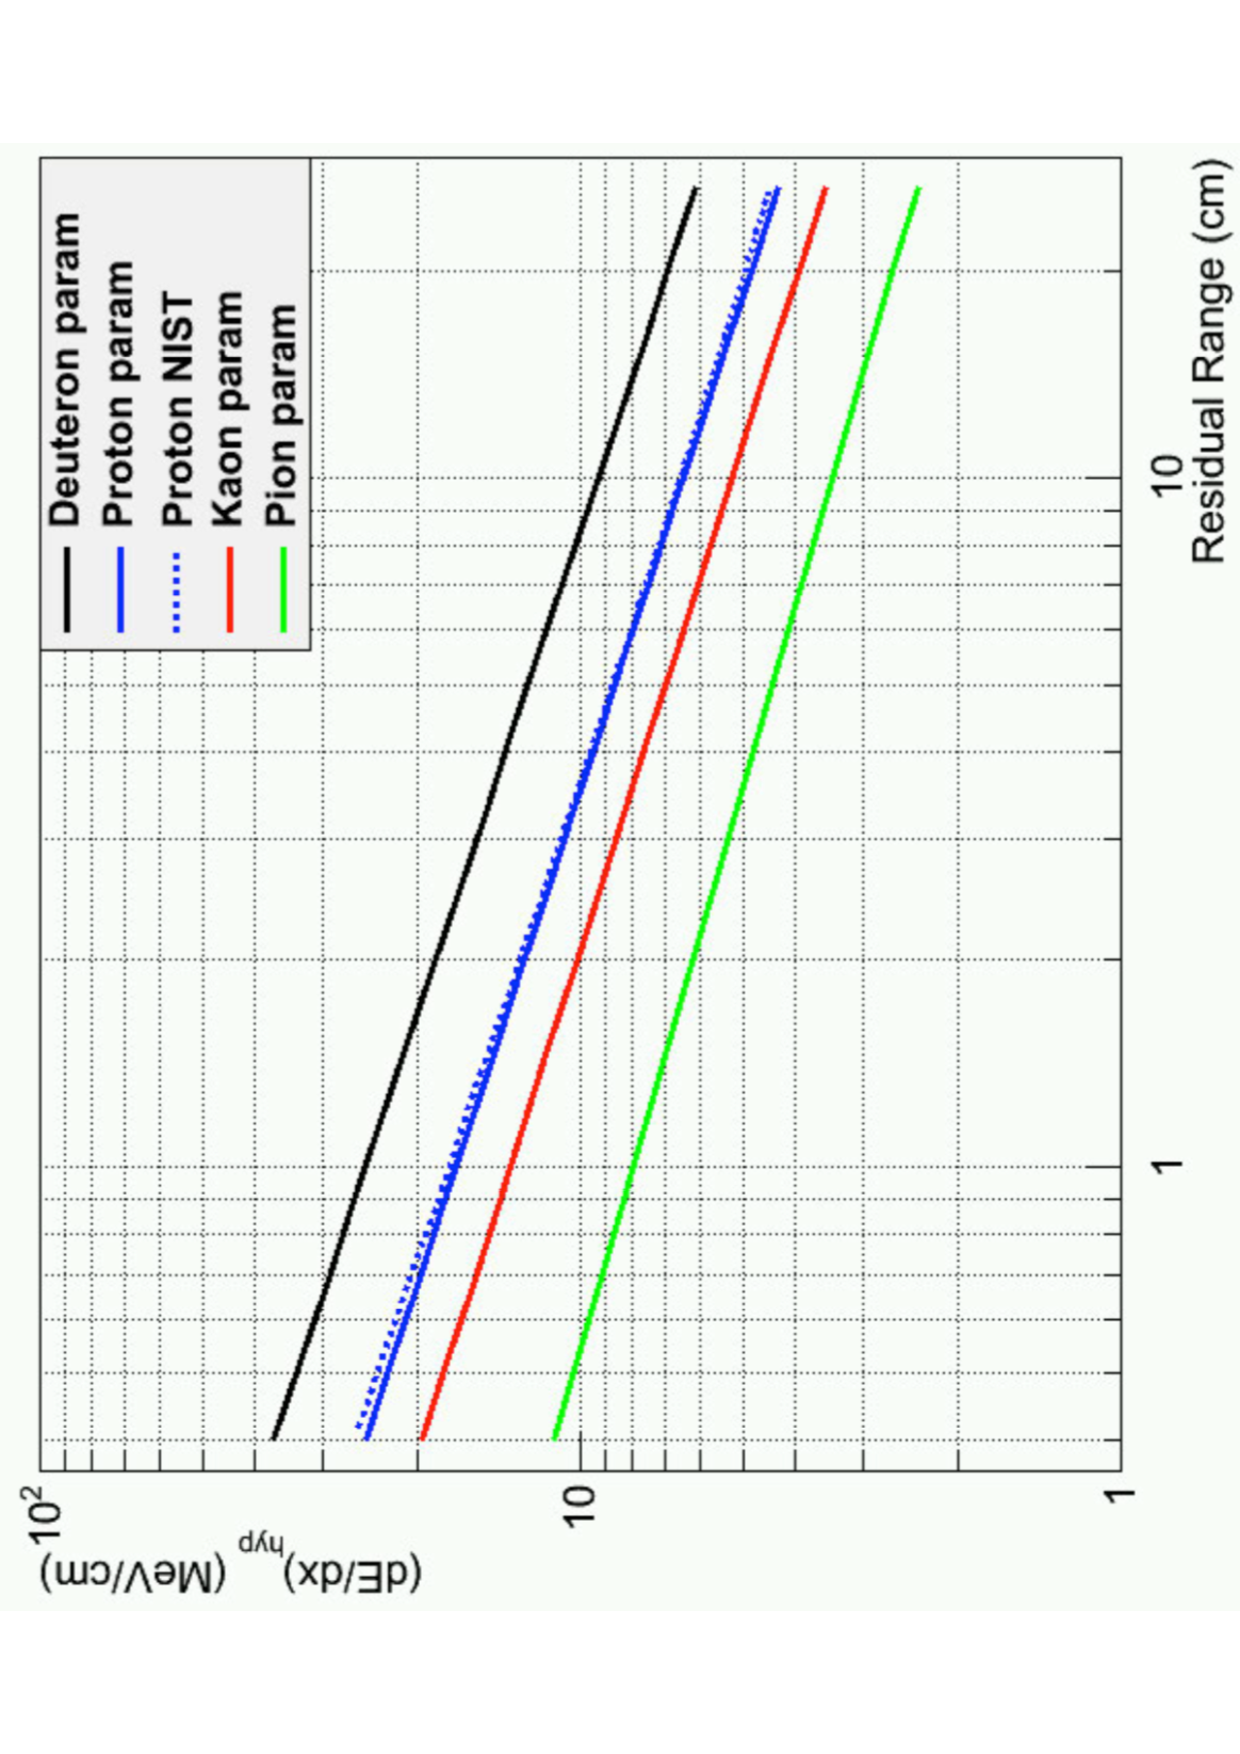
\includegraphics[width=\textwidth]{StoppingPower}
    \caption{Stopping power for different particle masses.}
    \label{fig:PIDA_loglog}
  \end{subfigure}
  \hspace{0.08\textwidth}
  \begin{subfigure}{0.45\textwidth}
    \centering
    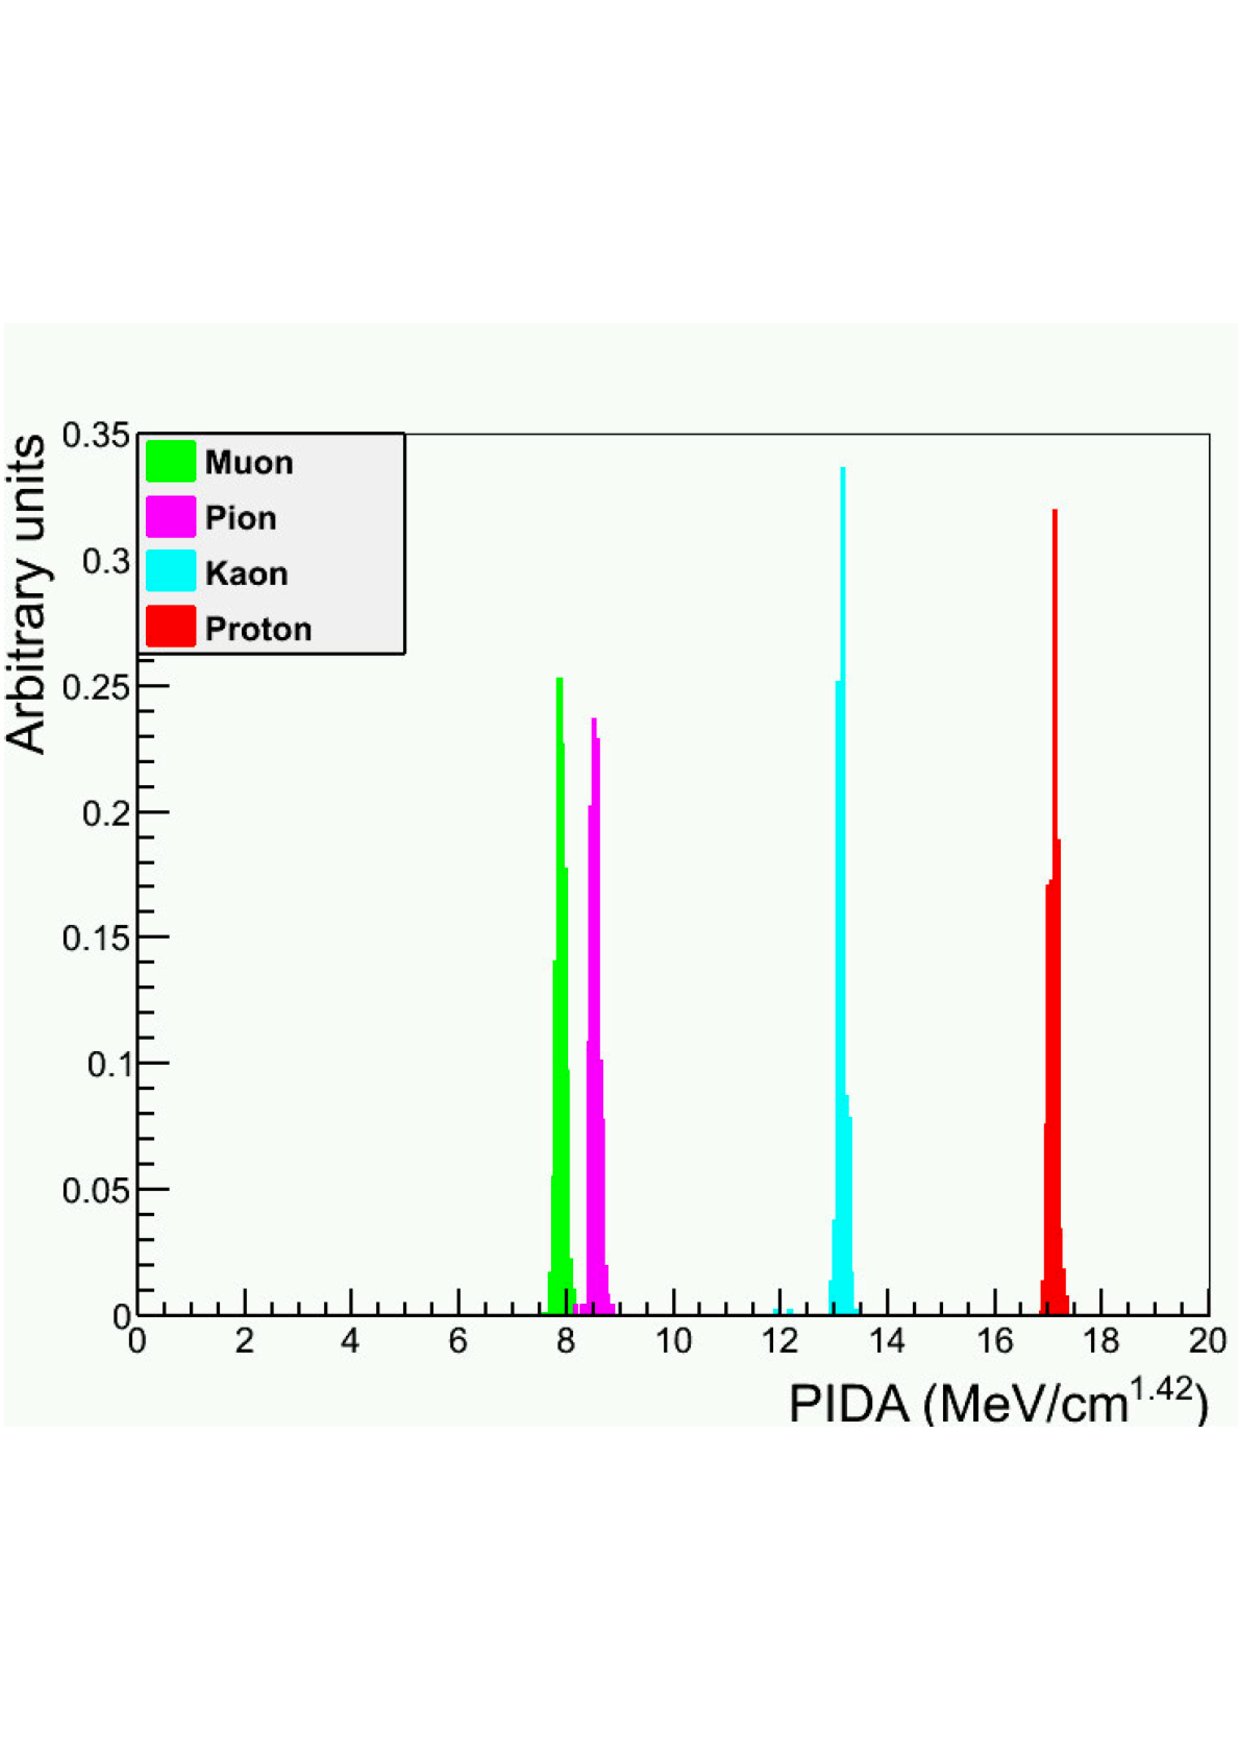
\includegraphics[width=\textwidth]{TruthPIDA}
    \caption{Distribution of PIDA values for different particle masses.}
    \label{fig:PIDA_MC}
  \end{subfigure}
  \caption[Defining the PIDA metric for particle identification.]
          {Defining the PIDA metric for particle identification and testing it on a Monte Carlo sample using truth information.}
          \label{fig:PIDAPlots}
\end{figure}

From Figure~\ref{fig:PIDAPlots} it can be seen that the most distinct PIDA distributions are that of muons and protons, these are also two of the most common particle types in cosmic rays. For these reasons particle identification using the PIDA variable will be attempted on simulations of the 35 ton. As outlined in Sections~\ref{sec:SimInteractionTimes} and ~\ref{sec:MCCalib} in order to do this the interaction times of particles have to be well known and the calibration constants must be tuned so as to ensure that the effects of recombination are properly accounted for. It is also useful to use the information found in Section~\ref{sec:SimRecoEffic} about the efficiency with which tracks are reconstructed. In this regard it is useful to produce additional figures showing the reconstruction efficiencies of protons in the CRY sample, these are shown in Figure~\ref{fig:Prot_Effic}.\\

\begin{figure}[h!]
  \centering
  \begin{subfigure}{.45\textwidth}
        \centering
        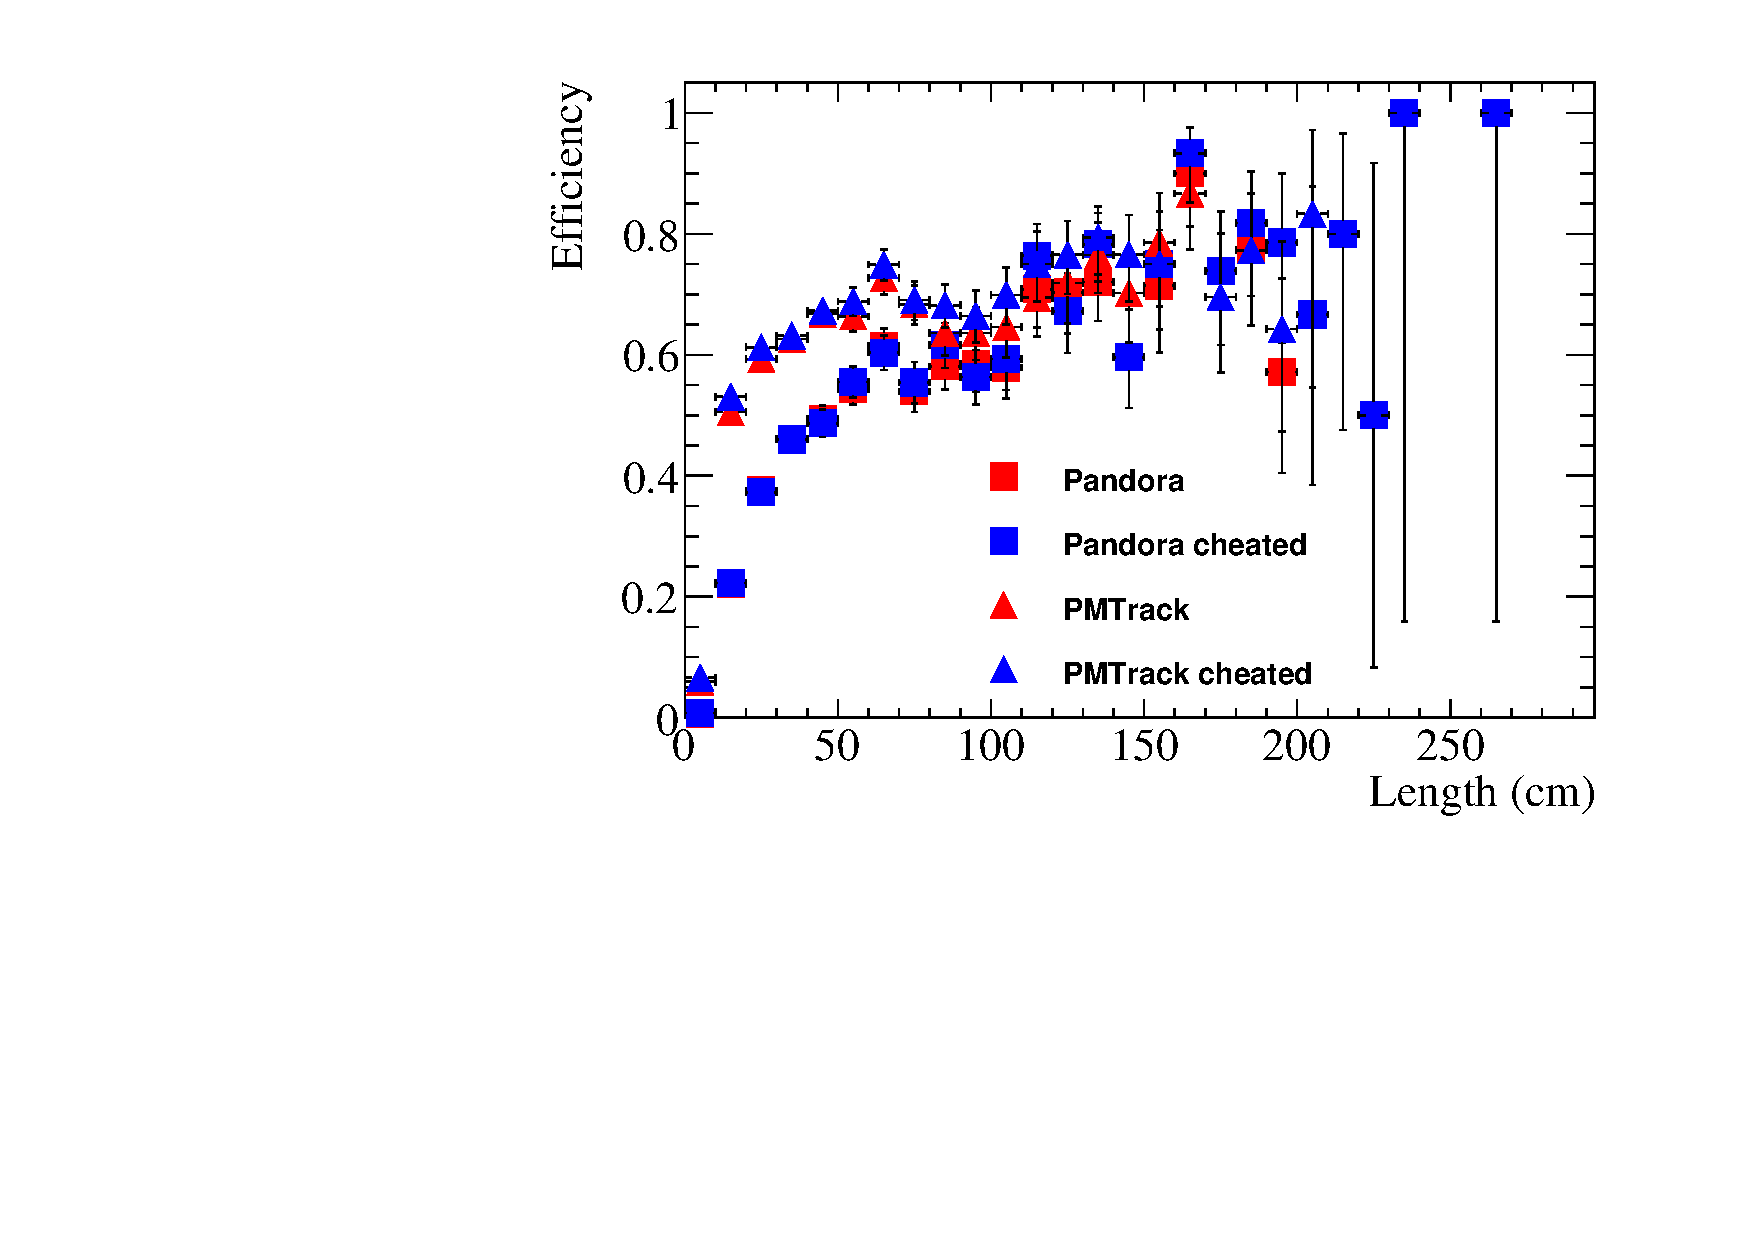
\includegraphics[width=\textwidth]{Effic_ProtonEnrich_500V_Proton_Length}
        \caption{The reconstruction efficiency as a function of Monte Carlo truth track length.}
        \label{fig:Prot_Effic_Len}
  \end{subfigure}
  \hspace{0.08\textwidth}
  \begin{subfigure}{.45\textwidth}
        \centering
        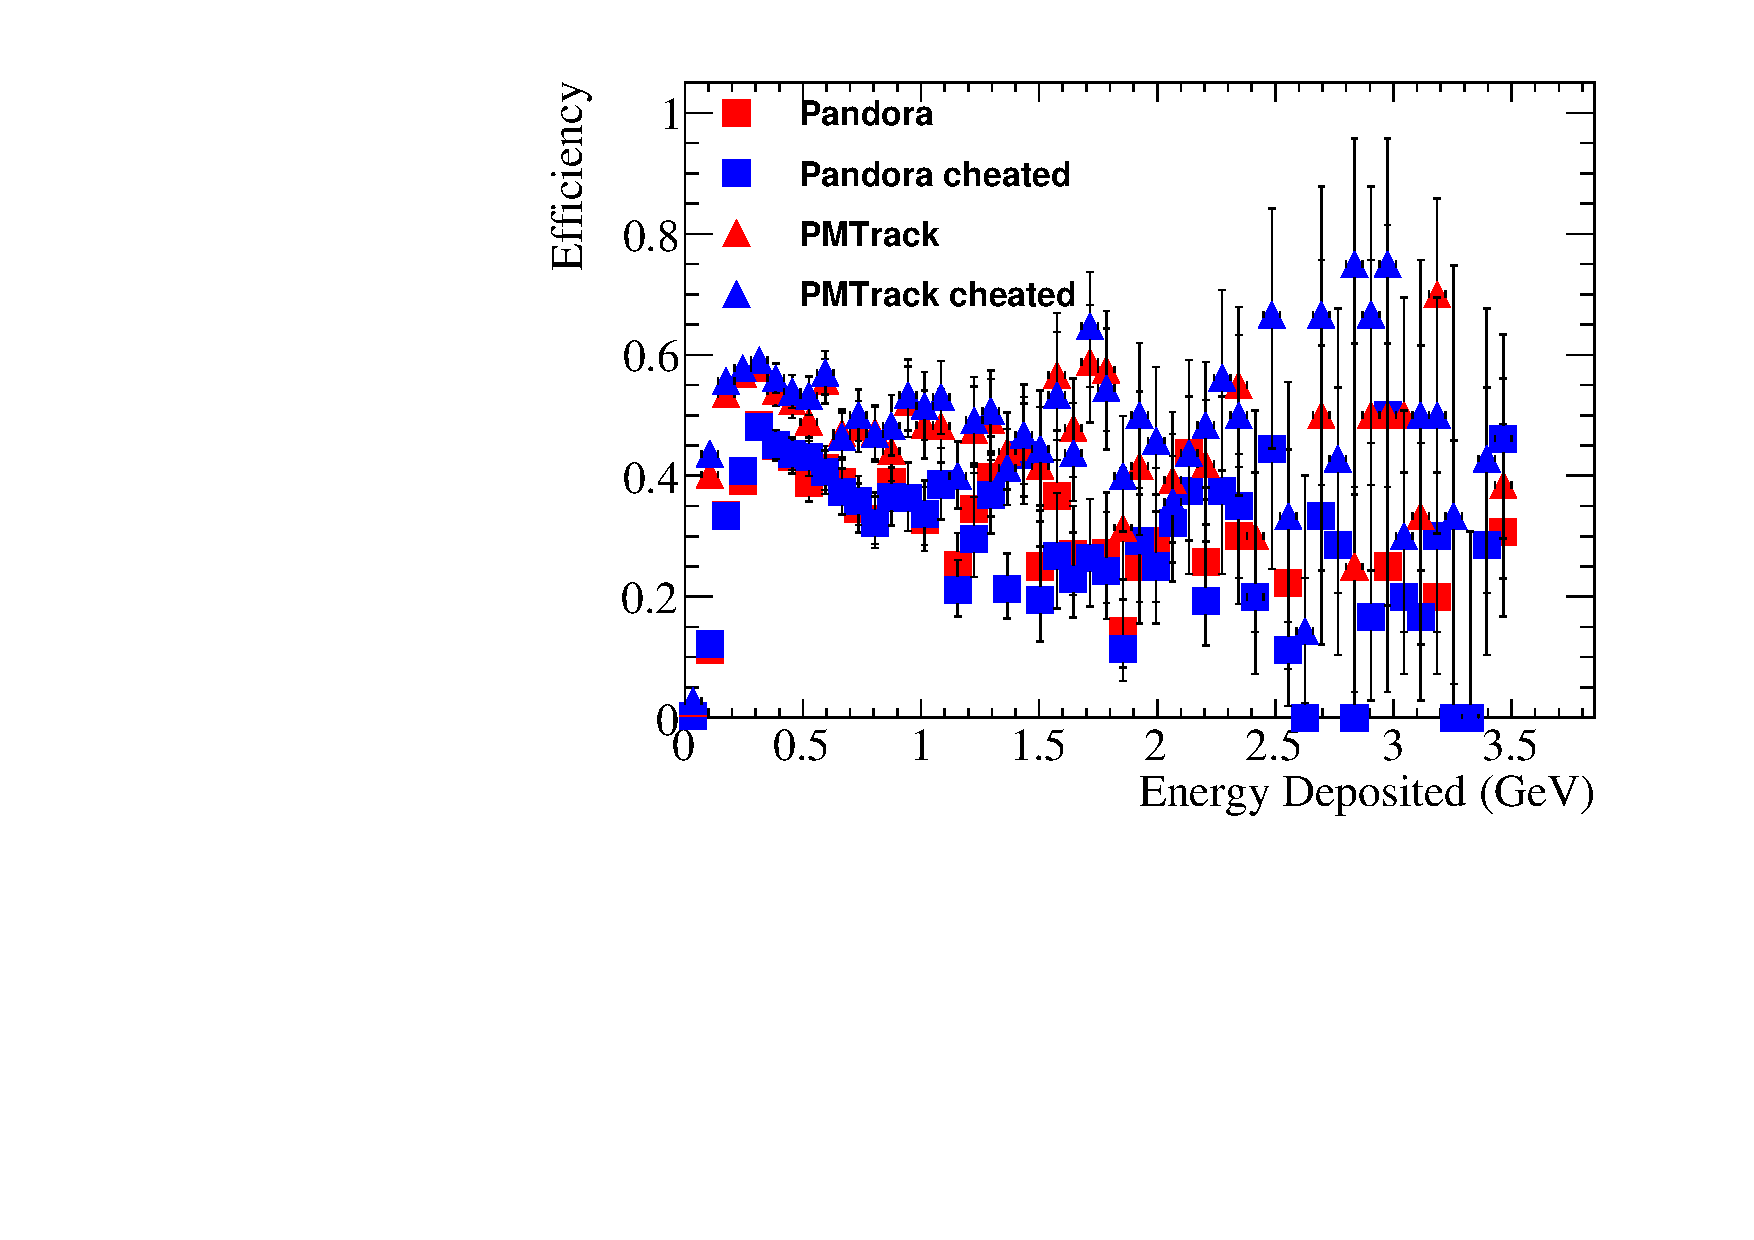
\includegraphics[width=\textwidth]{Effic_ProtonEnrich_500V_Proton_EnDepos}
        \caption{The reconstruction efficiency as a function of Monte Carlo truth deposited energy.}
        \label{fig:Prot_Effic_EnDepos}
  \end{subfigure}
  \begin{subfigure}{.45\textwidth}
        \centering
        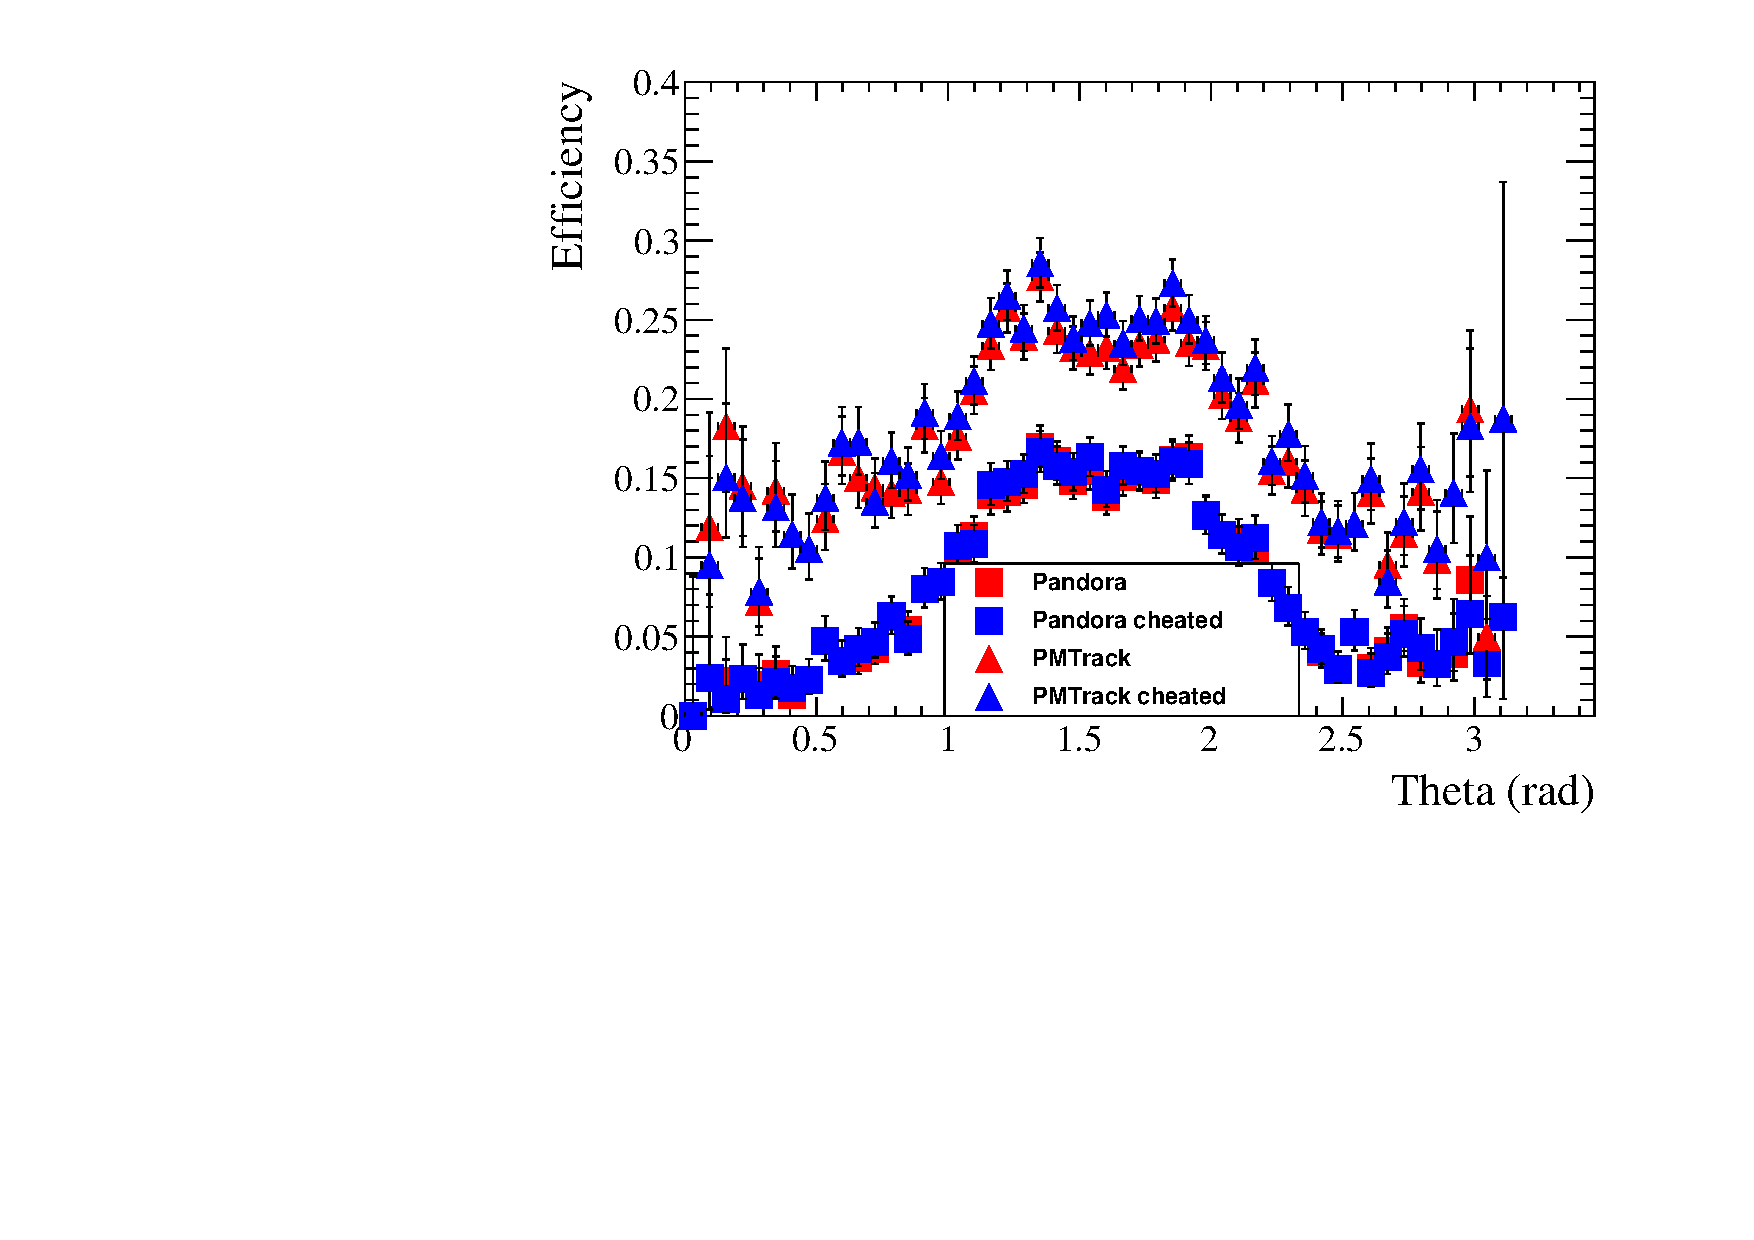
\includegraphics[width=\textwidth]{Effic_ProtonEnrich_500V_Proton_Theta}
        \caption{The reconstruction efficiency as a function of Monte Carlo truth track angle in theta.}
        \label{fig:Prot_Effic_Theta}
  \end{subfigure}
  \hspace{0.08\textwidth}
  \begin{subfigure}{.45\textwidth}
        \centering
        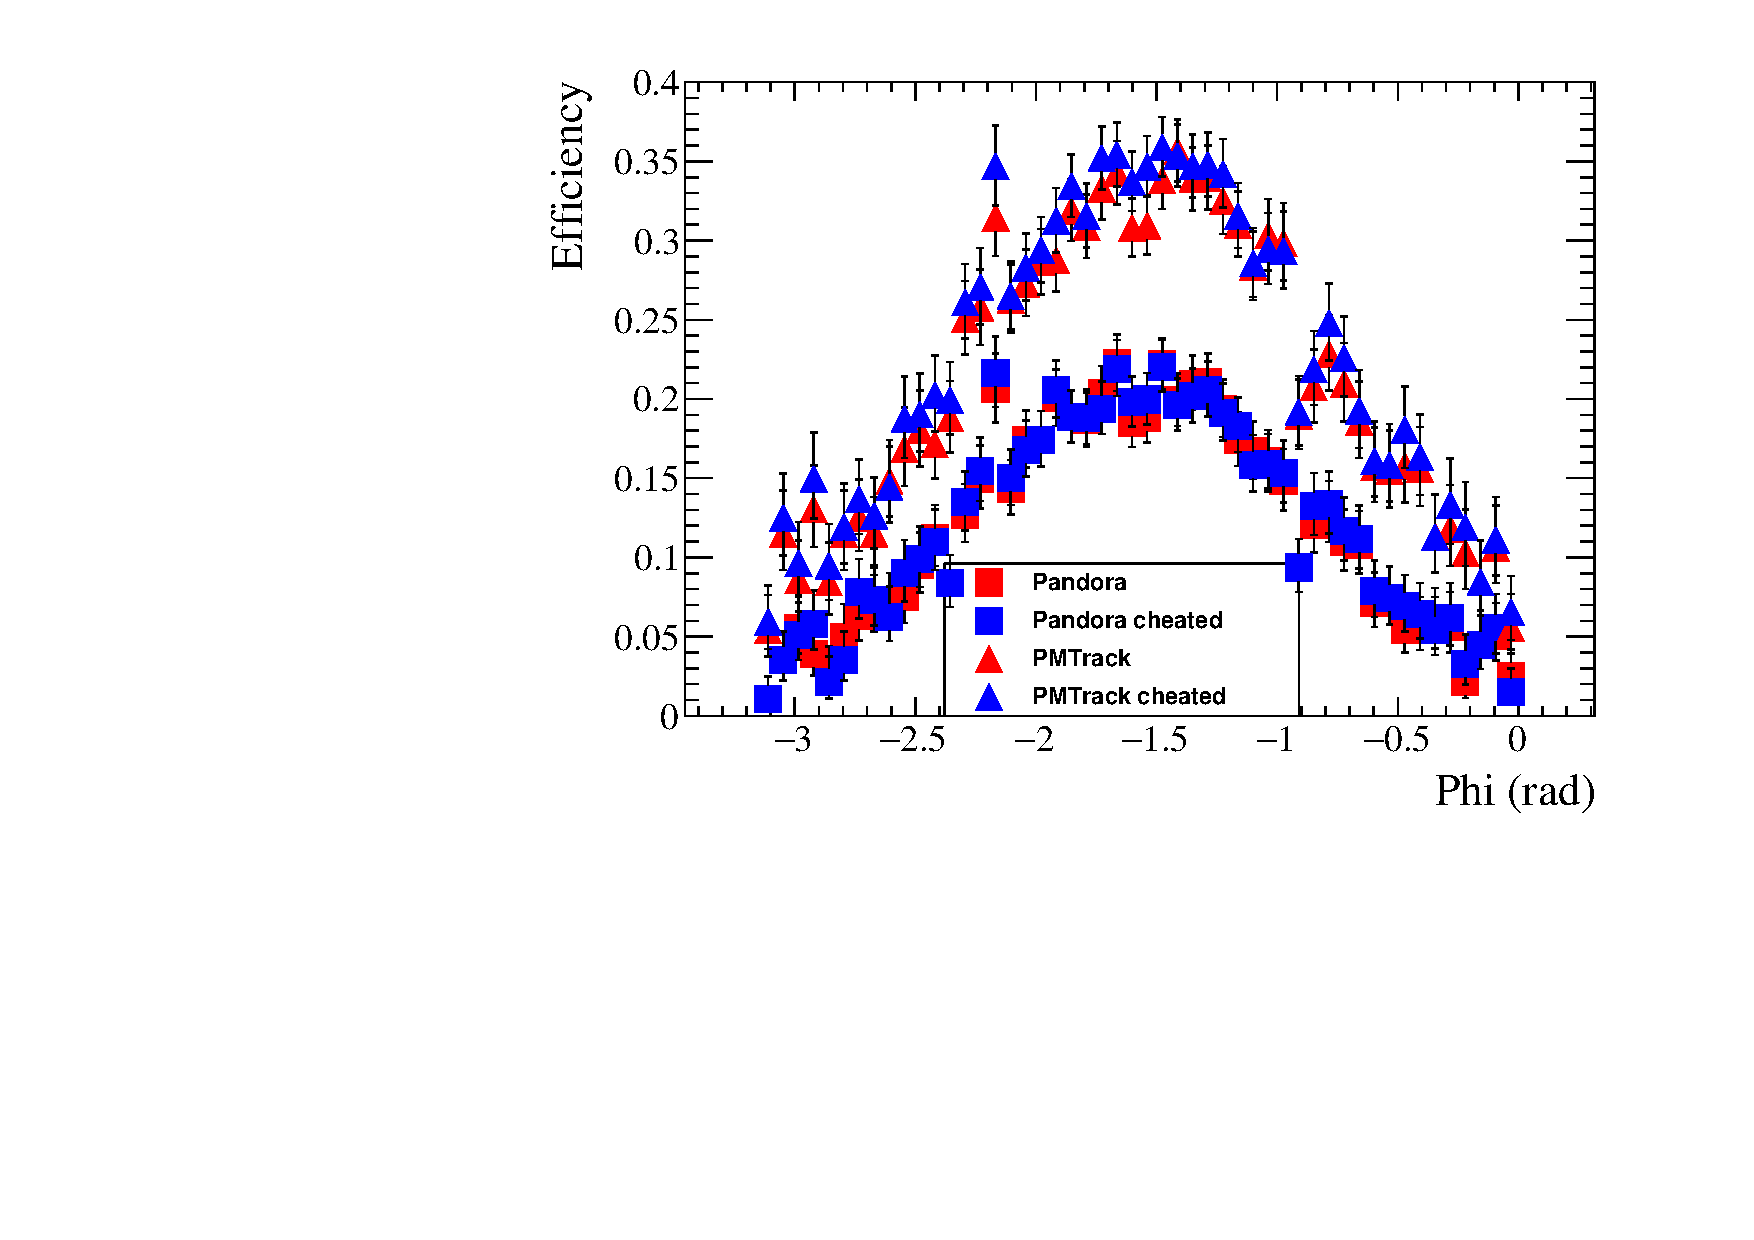
\includegraphics[width=\textwidth]{Effic_ProtonEnrich_500V_Proton_Phi}
        \caption{The reconstruction efficiency as a function of Monte Carlo truth track angle in phi.}
        \label{fig:Prot_Effic_Phi}
  \end{subfigure}
  \begin{subfigure}{.45\textwidth}
        \centering
        \includegraphics[width=\textwidth]{Effic_ProtonEnrich_500V_Proton_PhiTheta}
        \caption{The reconstruction efficiency as a function of Monte Carlo truth track angle in theta and phi.}
        \label{fig:Prot_Effic_PhiTheta}
  \end{subfigure}
  \caption[The reconstruction efficiencies for protons in a sample generated using CRY.]
          {The reconstruction efficiencies for protons in a sample generated using CRY. The efficiencies are shown for non-cheated reconstruction (square blocks) and cheated reconstruction (triangle blocks) for both PMTrack (black) and Pandora (blue).}
  \label{fig:Prot_Effic}
\end{figure}

Figure~\ref{fig:Prot_Effic} shows that the average reconstruction efficiency for PMTrack is higher than that for Pandora when considering protons, as the efficiency for the former is roughly 10\% higher for all angles as shown in Figure~\ref{fig:Prot_Effic_Theta}, though it is much lower than the overall efficiency seen in Figure~\ref{fig:SimEffic_Theta_CRY}. From Figure~\ref{fig:Prot_Effic_Len} it is evident that the efficiency for protons with track lengths of more than 10 cm is similar to that of the overall efficiency for the CRY sample, but the efficiency for the shortest tracks is significantly lower than that of the whole CRY sample. A review of the true path lengths of the simulated particles shows that 60\% of the protons have path lengths of less than 1 cm and that none of these particles were reconstructed, it is this large number of very short particles which causes the overall reconstruction to be relatively low. When a minimum path length of 1 cm (10 cm) is required the reconstruction efficiency rises to 37\% (58\%), so when the shortest tracks are not counted the reconstruction performs well. \\

It is also useful to produce samples where the primary particle is a single muon or proton located in the active volume of the detector. This allows for a sample of isolated tracks to be made upon which the capabilities of the PIDA metric can be tested. It also allows the reconstruction efficiency to be found for particles in isolation. The properties of the particles generated are illustrated below in Table~\ref{tab:IsolProp}. The values of the simulated quantities were found by changing the given parameters by an amount taken from a random sampling of a Gaussian distribution of width equal to the error listed. These simulation parameters were chosen to produce samples which would contain both exiting and stopping particles whilst generating the particles in the LAr would ensure that there was always a reconstructable track in the detector. \\

The reconstruction efficiencies when using the PMTrack reconstruction method is shown for the simulated particles in Figure~\ref{fig:Isol_Effic}. SOME SPLAININGS ABOUT THAT SAMPLE!!!! \\

\begin{table}
\caption{The properties of initial particles simulated in the muon and proton samples.}
\centering
\label{tab:IsolProp}
\begin{tabular}{l c c}
\toprule
{} & {Muon properties} & {Proton properties} \\ 
\midrule
Initial position (cm)              & (100 $\pm$ 50, 0 $\pm$ 30, 80 $\pm$ 20) & (100 $\pm$ 50, 0 $\pm$ 30, 80 $\pm$ 20)  \\

Initial momentum (GeV)            & 0.3 $\pm$ 0.1 & 0.8 $\pm$ 0.5 \\

Initial $\theta_{XZ}$ $(^{\circ})$ &   0 $\pm$ 180 &   0 $\pm$ 180 \\

Initial $\theta_{YZ}$ $(^{\circ})$ & -45 $\pm$ 45  & -45 $\pm$ 45  \\
\bottomrule
\end{tabular}
\end{table}

\begin{figure}[h!]
  \centering
  \begin{subfigure}{.45\textwidth}
        \centering
        %\includegraphics[width=\textwidth]{Effic_ProtonEnrich_500V_Proton_Length}
        \caption{The reconstruction efficiency as a function of Monte Carlo truth track length.}
        \label{fig:Isol_Effic_Len}
  \end{subfigure}
  \hspace{0.08\textwidth}
  \begin{subfigure}{.45\textwidth}
        \centering
        %\includegraphics[width=\textwidth]{Effic_ProtonEnrich_500V_Proton_EnDepos}
        \caption{The reconstruction efficiency as a function of Monte Carlo truth deposited energy.}
        \label{fig:Isol_Effic_EnDepos}
  \end{subfigure}
  \begin{subfigure}{.45\textwidth}
        \centering
        %\includegraphics[width=\textwidth]{Effic_ProtonEnrich_500V_Proton_Theta}
        \caption{The reconstruction efficiency as a function of Monte Carlo truth track angle in theta.}
        \label{fig:Isol_Effic_Theta}
  \end{subfigure}
  \hspace{0.08\textwidth}
  \begin{subfigure}{.45\textwidth}
        \centering
        %\includegraphics[width=\textwidth]{Effic_ProtonEnrich_500V_Proton_Phi}
        \caption{The reconstruction efficiency as a function of Monte Carlo truth track angle in phi.}
        \label{fig:Isol_Effic_Phi}
  \end{subfigure}
  \begin{subfigure}{.45\textwidth}
        \centering
        %\includegraphics[width=\textwidth]{Effic_ProtonEnrich_500V_Proton_PhiTheta}
        \caption{The reconstruction efficiency as a function of Monte Carlo truth track angle in theta and phi.}
        \label{fig:Isol_Effic_PhiTheta}
  \end{subfigure}
  \caption[The reconstruction efficiencies for single muons and protons in the 35 ton.]
          {The reconstruction efficiencies for single muons and protons in the 35 ton. The efficiencies are shown for non-cheated reconstruction (square blocks) and cheated reconstruction (triangle blocks) for both muons (black) and protons (blue).}
  \label{fig:Isol_Effic}
\end{figure}

As the increase in $\frac{dE}{dx}$ is only visible when the particle stops in the detector it is necessary to remove exiting particles from the sample by applying a fiducial cut cut on the end point of the reconstructed track. It is important to only place this on the end point of the track, as one does not want to remove particles which enter the detector and then stop. When calorimetry is performed the end point of the track is determined using, among other metrics, the increase in $\frac{dE}{dx}$ and so the residual range of the track (a stored data member of the track object) should always refer to the end of the particles trajectory. For this study a fiducial cut of 5 cm is used as this means that a large section of an exiting track would have to be mistaken for a stopping particle. This will reduce the sample size, but it is necessary to ensure that exiting particles are not included in the final distributions. A further cut that is applied is the requirement that there are a minimum of 10 continuous collection plane hits, this is to ensure that an adequate number of points are taken upon which to find an average value of PIDA for the track. Similar cuts are described in~\citep{PIDA_Paper}, and the resulting distributions of PIDA values for the single proton and muon samples are shown in Figure~\ref{fig:Isol_PIDA}. \\

\begin{figure}[h!]
  \centering
  \begin{subfigure}{.45\textwidth}
        \centering
        \includegraphics[width=\textwidth]{IsolatedProtons_500V_Dec16_Proton_PIDA}
        \caption{The PIDA values calculated for the single proton sample.}
        \label{fig:Isol_PIDA_Proton}
  \end{subfigure}
  \hspace{0.08\textwidth}
  \begin{subfigure}{.45\textwidth}
        \centering
        \includegraphics[width=\textwidth]{IsolatedMuons_500V_Dec16_Muon_PIDA}
        \caption{The PIDA values calculated for the single muon sample.}
        \label{fig:Isol_PIDA_Muon}
  \end{subfigure}
  \caption[The calculated PIDA values for single muons and protons in the 35 ton.]
          {The calculated PIDA values for single muons and protons in the 35 ton. A series of criteria designed to select only tracks due to stopping particles which have a required number of collection plane hits is applied. The tracks are then further refined using truth information such as the true end point of the particle.}
  \label{fig:Isol_PIDA}
\end{figure}

As can be seen from Figure~\ref{fig:Isol_PIDA} using truth information can make the distributions much cleaner, particularly when discounting particles for which the reconstruction algorithms do not track to their end point. It is reassuring to see that few tracks are reconstructed backwards, as if this were not the case then performing particle identification would be very difficult as it would indicate that the calorimetry and tracking algorithms are not performing well. Improvements can still be made though, as both plots in Figure~\ref{fig:Isol_PIDA} contain tracks which do not have the final energy depositions. This can seen as when tracks which do not match with the true end points of the particles are removed the low tails of the PIDA distributions are significantly reduced. It is observed that the PIDA distributions are cleaner when information from all three wire planes are used as opposed to only using the collection plane. This shows how important it is to calibrate the electronics response of all three wire planes and how additional wire planes can improve calorimetry as well as the accuracy of reconstruction algorithms. \\

The relationship between the $\frac{dE}{dx}$ and residual range of a track is shown in Figure~\ref{fig:Isol_dEdx} for both protons and muons. The much steeper increase in $\frac{dE}{dx}$ at low residual range for protons compared to muons is clearly visible when comparing Figures~\ref{fig:Isol_dEdx_Proton} and~\ref{fig:Isol_dEdx_Muon}. The contamination in the proton sample at low PIDA can be seen in Figure~\ref{fig:Isol_dEdx_Proton} where there is a clear sample of tracks for which the $\frac{dE}{dx}$ does not increase for low residual ranges. These plots are filled after tracks which do not correlate to the ends of the true trajectories are removed, and so the tail of low $\frac{dE}{dx}$ values is due to particles for which the simulated detector did not find increased energy depositions as the particle stopped. It is interesting to note that when a simple version of PIDA is calculated using the MC truth energy deposits, shown in Figure~\ref{fig:MCPIDA}, these particles are also found to have low value of PIDA. It is therefore possible that at least some of these protons do not in fact stop, but interact when they still have a significant amount of kinetic energy, though some tracks which have a low truth PIDA have the expected PIDA when using reconstructed information. \\

\begin{figure}[h!]
  \centering
  \begin{subfigure}{.45\textwidth}
        \centering
        \includegraphics[width=\textwidth]{IsolatedProtons_500V_Dec16_Proton_dEdx}
        \caption{The $\frac{dE}{dx}$ versus residual range plot for the single proton sample.}
        \label{fig:Isol_dEdx_Proton}
  \end{subfigure}
  \hspace{0.08\textwidth}
  \begin{subfigure}{.45\textwidth}
        \centering
        \includegraphics[width=\textwidth]{IsolatedMuons_500V_Dec16_Muon_dEdx}
        \caption{The $\frac{dE}{dx}$ versus residual range plot for the single muon sample.}
        \label{fig:Isol_dEdx_Muon}
  \end{subfigure}
  \caption[The $\frac{dE}{dx}$ versus residual range plot for single muons and protons in the 35 ton.]
          {The measured relationship between $\frac{dE}{dx}$ and residual range for single muons and protons in the 35 ton. The plots are made after applying all of the cuts outlined in Figure~\ref{fig:Isol_PIDA}, meaning that the MIP peaks have been suppressed using truth information.}
  \label{fig:Isol_dEdx}
\end{figure}

\begin{figure}[h!]
  \centering
  \includegraphics[width=0.5\textwidth]{IsolatedProtons_500V_Dec16_Proton_MCPIDA_PIDA}
  \caption[A comparison between PIDA values calculated using truth and reconstructed information]
          {A comparison between PIDA values calculated using truth and reconstructed information}
  \label{fig:MCPIDA}
\end{figure}

It is useful to summarise the information shown in Figure~\ref{fig:Isol_PIDA} in a table so that an efficiency of identifying stopping particles can be found. This is shown in Table~\ref{tab:Isol_PIDA_Proton} for protons, and in Table~\ref{tab:Isol_PIDA_Muon} for muons. The PIDA ranges referred to are 14-18 and 6-10 for the protons and muons respectively. As can be seen in Table~\ref{tab:Isol_PIDA_Proton} the efficiency upon which protons can be identified does not change significantly as the sequential criteria are applied, but as shown in Figure~\ref{fig:Isol_PIDA_Proton} the low PIDA peak decreases significantly. The same cannot be said for the muon sample however where the criteria that the tracking end point matches the true end point as that removes a significant section of the tail within the PIDA range, but the resulting distribution is more similar to the distribution shown in Figure~\ref{fig:PIDA_MC}. Though the cut to remove tracks which do not have the correct end points reduces the efficiencies, should all the tracks be reconstructed with the correct end points then one can imagine that the number of tracks within the PIDA range would increase and the distributions would become more symmetrical as shown in Figure~\ref{fig:Isol_PIDA_Muon}. \\

\begin{table}
  \caption[A summary of the PIDA values calculated for the proton sample as sequential cuts are applied]
          {A summary of the PIDA values calculated for the proton sample as sequential cuts are applied.}
  \centering
  \label{tab:Isol_PIDA_Proton}
  \begin{tabular}{l c c c}
    \toprule
    \multirow{2}{*}{Applied cut} & \multicolumn{3}{c}{Proton sample} \\ 
    \cmidrule{2-4}
      & Tracks & In PIDA range & Efficiency \\ 
    \midrule
      Total stopping particles            & 9000 &      &      \\

      Reconstructed tracks                & 8000 & 5000 & 55\% \\

      Survives 5 cm fiducial cut          &      &      &      \\

      Minimum of 10 collection plane hits &      &      &      \\

      Correct track orientation           &      &      &      \\

      Correct tracking end point          &      &      &      \\
    \bottomrule
  \end{tabular}
\end{table}

\begin{table}
  \caption[A summary of the PIDA values calculated for the proton sample as sequential cuts are applied]
          {A summary of the PIDA values calculated for the proton sample as sequential cuts are applied.}
  \centering
  \label{tab:Isol_PIDA_Muon}
  \begin{tabular}{l c c c}
    \toprule
    \multirow{2}{*}{Applied cut} & \multicolumn{3}{c}{Muon sample} \\ 
    \cmidrule{2-4}
      & Tracks & In PIDA range & Efficiency \\ 
    \midrule
      Total stopping particles            & 9000 &      &      \\

      Reconstructed tracks                & 8000 & 5000 & 55\% \\

      Survives 5 cm fiducial cut          &      &      &      \\

      Minimum of 10 collection plane hits &      &      &      \\

      Correct track orientation           &      &      &      \\

      Correct tracking end point          &      &      &      \\
    \bottomrule
  \end{tabular}
\end{table}

Upon verifying that the PIDA metric can reliably determine particle type when they are simulated in isolation, the next step is to observe the accuracy upon which particles can be identified in a CRY sample. The sample used here differs from the CRY sample used earlier in that only event which contain a proton in the detector are reconstructed, this is done to reduce simulation time and storage space as this cut will still provide a substantial number of muons whilst ensuring that a large proton sample can be reconstructed. The process of calculating PIDA values for the tracks is identical in all samples, though as discussed in Section~\ref{sec:SimRecoEffic} the much more complicated event structure in the CRY sample affects the reconstruction efficiency and so will likely also affect the accuracy of the calorimetry. The calorimetry will be affected in two ways, firstly the reduced performance of the reconstruction algorithms will mean that some particles are not reconstructed at all, whilst those that are reconstructed may be more likely to have missing hits meaning that the end points may be less well reconstructed. This will cause the tail of low $\frac{dE}{dx}$ values seen in Figure~\ref{fig:Isol_dEdx_Proton} to be more pronounced. Secondly, as shown in Figure~\ref{fig:PD_MCPDDiff} though the photon detector time determination is very accurate for a large number of tracks it is also incorrect for a large number of tracks, this will cause the recombination correction to be miscalculated which will in turn increase the calculated $\frac{dE}{dx}$ and hence PIDA values. \\

The PIDA values calculated for protons and muons in the CRY sample are shown in Figure~\ref{fig:CRY_PIDA}. As can be seen from Figure~\ref{fig:CRY_PIDA_Muon} there is a tail of very high PIDA value muon tracks which contaminate the proton PIDA region of interest (ROI). This causes a serious problem when trying to identify protons from a cosmic sample as the number of muons present is significantly larger than the number of protons. The result of this will be a sample of tracks which will not be very pure, and so further cuts will have to be devloped to enhance the purity of this sample whilst not reducing the efficiency upon which proton tracks are identified. 

\begin{figure}[h!]
  \centering
  \begin{subfigure}{.45\textwidth}
        \centering
        %\includegraphics[width=\textwidth]{}
        \caption{The PIDA values calculated for the single proton sample.}
        \label{fig:CRY_PIDA_Proton}
  \end{subfigure}
  \hspace{0.08\textwidth}
  \begin{subfigure}{.45\textwidth}
        \centering
        %\includegraphics[width=\textwidth]{}
        \caption{The PIDA values calculated for the single muon sample.}
        \label{fig:CRY_PIDA_Muon}
  \end{subfigure}
  \caption[The calculated PIDA values for muons and protons in a CRY sample through the 35 ton]
          {The calculated PIDA values for muons and protons in a CRY sample through the 35 ton. A series of criteria designed to select only tracks due to stopping particles which have a required number of collection plane hits is applied. The tracks are then further refined using truth information such as the true end point of the particle.}
  \label{fig:CRY_PIDA}
\end{figure}

%*******************************************************************************
%*********************************** Chapter XXXXXXXX *****************************
%*******************************************************************************
\chapter{The 35 ton data sample} \label{chap:35tonData} %Title of chapter
  
\graphicspath{{35tonData/Figs/PDF/}{35tonData/Figs/Raster/}{35tonData/Figs/Vector/}}

The data taking period for the 35 ton prototype was from November 2015 until March 2016. This included an extensive commissioning period before the detector was filled with LAr, and the electric field was turned on. During this time many of the features of the data discussed below were first noticed, and attempts to rectify these were pursued. A long commissioning period was also required because many of the DAQ sub-systems were still under active development in November.\\

A total of 22 days worth of data was collected with the electric field set at 250 V cm$^{-1}$, the breakdown of when these periods occurred is shown in Figure~\ref{fig:DataCollected}. It is clear that the analysable data is interspersed with data where the electric field was not turned on, this is both due to extenuating circumstances such as a site wide power outage in early March, and a dedicated two week noise hunting exercise in February. The physics data taking period ended at 3am on 19th March 2016, when a filtration pump broke causing an unrecoverable loss of purity as air was pumped into the detector. Following this studies to understand the electronics noise and to test the high voltage systems continued, but it was deemed too costly to acquire any more physics data. During this time the electric field was raised to the nominal value of 500  V cm$^{-1}$, and some of the causes of the higher than expected noise levels were discerned. \\

\begin{figure}
  \centering
  \includegraphics[width=1.0\textwidth]{DataCollected}
  \caption[The 35 ton data sample]{Timeline showing the data collected during the 35 ton Phase II run once the purification pumps were turned on.}
  \label{fig:DataCollected}  
\end{figure}

%********************************** %First Section  **************************************
\section{Organisation of the data structure} \label{Organisation of the data structure} %Section - X.1
As previously noted the 35 ton consisted of three detector sub-systems: RCEs collecting TPC data, SSPs collecting photon detector data, and CRCs tagging cosmic rays. The DAQ combined these three data streams into synchronous events in time and saved them as LArSoft data objects. These data objects would later have to be converted to the offline data products, which the reconstruction tools developed on simulation used, this is discussed in Section~\ref{Reformatting the data to the offline structure}. This section describes the structure of the data objects in the raw form.\\

During operations the DAQ was configured to maximise data throughput and physics potential. This meant recording different lengths of times for each of the three sub-systems, as the data volumes and length of physics information were significantly different. For example, due to the emission of prompt light, the physics information from the SSPs is of a much shorter length of time than the physics information from the RCEs, where data has to be recorded whilst the electrons drift through the LAr. During the running period the recorded data was triggered by through-going muons which produced coincidences on the CRCs on opposites side of the cryostat. A coincidence is defined as two CRC modules recording a hit within 32 ns. The system used to collect the CRC data was also responsible for generating the triggers, and so this meant that the trigger rate could be suppressed to approximately 1 Hz, by only producing triggers every N times a coincidence occurred, where N was a tuneable variable. A trigger rate of 1 Hz was used as the maximum speed at which data could be written to disk was approximately 60 MB s$^{-1}$, which is roughly equal to the size of each triggered event when the entire detector is read-out in the configuration discussed below. The rate at which events were recorded could have been increased if zero-suppression of the TPC data had been used, however the noise level meant that this was not feasible. \\ 

With an electric field of 250 V cm$^{-1}$, and a drift of 2.25 m, the drift time for electrons at the long drift CPA was roughly 2.6 ms or 5200 ticks (where 1 tick is 500 ns). It was decided that in order for a track causing a counter coincidence to be separated from other tracks, it was necessary to have roughly one drift window both before, and after, the drift window around the coincidence. This means that data was recorded for 7.5 ms, or 15,000 ticks, around each coincidence. The SSPs only collected the prompt light from through-going particles, and so only 200 $\mu$s of SSP data was recorded for each event. The CRCs produced the least volume of data, and so were able to be read out constantly. \\

As the run mode required accessing buffered data, it had to be discretised inside the components before being sent to the event builders in the DAQ. In the discussion of how this worked, focus will be given on the RCE data where some new terms need to be introduced. The smallest unit of data, called a nanoslice, is the data from one RCE for one tick, where each RCE controls 128 channels meaning that there were a total of 16 RCEs in the 35 ton. A microslice is then made by combining 1000$\times$N nanoslices such that it contains 0.5 ms (1,000 ticks) of data across all channels, where N is the number of RCEs that are recorded in the run. Microslices are then combined to make millislices, the length of which was configurable. Once produced, these millislices were sent by the DAQ to the event builders, to be stored as time synchronous LArSoft data objects. \\

The time synchronous events produced by the DAQ, did not, however, correspond to the physics events. This is because the DAQ was originally designed to produce a continuous data stream. This meant that the DAQ was configured to pad events with headers when a sub-system provided no physics information, such as nanoslices in the case of the RCEs. Removing these padded header objects was a remit of the online to offline converter discussed in Section~\ref{Reformatting the data to the offline structure}. As the length of the millislices was configurable, it was chosen to be 10 ms (20,000 ticks), in order to best attempt to fully contain physics events, and reduce the need for the online to offline converter to stitch DAQ events together. The padding of millislices with headers between physics events introduced some peculiarities in the recorded data, such as millislices containing two parts of non-continuous data. This is shown in Figure~\ref{fig:DataStructure}, where the second millislice has no information for the time between the end of physics event 2, and the start of physics event 3.\\

\begin{figure}
  \centering
  \includegraphics[width=0.75\textwidth]{DataStructure}
  \caption[The 35 ton data structure]
          {A diagram of possible millislice structures for the TPC data recorded by the 35 ton. Each row represents a millislice, whilst each box represents a microslice. The vertical blue lines delineate each microslice, giving 20 microslices per millislice. Solid red and green boxes represent microslices with TPC data in them. A group of 15 continuous red and green boxes are the recorded ``physics events''. Green boxes represent triggers which were used, with the black lines showing the time in the millislice at which the trigger occurred. Green and black patterned boxes represent coincidences of CRCs which were not issued as triggers. A possible reason for these triggers not being issued, is their proximity to a previous coincidence trigger which was issued.}
  \label{fig:DataStructure}
\end{figure}

During normal data taking, the last N microslices are buffered in the RCEs so that if a trigger is issued, the previous millislices can be accessed before they are deleted. As the data is buffered in the form of microslices, previous microslices may only be accessed in whole. This means that a whole number of microslices must be loaded before the trigger, so when a trigger is issued part way through a microslice, the previous X microslices are sent to the event builders. As a result, there are always a minimum number of ticks both before (5,000 ticks), and after (9,000 ticks), the trigger, but the exact numbers can change by up to 1,000 ticks for a given event, depending on where in the microslice the trigger came. The result of this is that it is impossible to know the number of ticks before/after a given counter coincidence. This is shown in Figure~\ref{fig:DataStructure} where the black lines representing triggers, are seen to occur at different points within the microslices. For example, physics event 1 will have more data after the trigger than physics event 2 as the trigger occurs earlier in the triggered microslice.

%********************************** %Second Section  *************************************
\section{Reformatting the data to the offline structure} \label{Reformatting the data to the offline structure} %Section - X.2
Conversion of the data objects stored in the raw data to the data objects used in simulation required a suite of unpacking services to be written, the specifics of which are not discussed here. These all required a common interface through which to access the data and check that the timing of each component was consistent, so that a final LArSoft file for downstream use could be produced. This interface had the added role of producing complete physics events, meaning that it had to be able to combine multiple millislices and extract only the data containing the continuous physics events. \\

Following the unpacking of each of the sub-systems, the data reformatter would loop through the TPC ticks to see if a user defined set of conditions could be satisfied at that time. These conditions were usually whether an East-West or North-South counter coincidence occurred at that time, or if this millislice contained TPC data whilst the previous one did not. The latter was the default configuration as this gave the option of preserving all of the data gathered, for reasons discussed at the end of Section~\ref{Organisation of the data structure}. Other conditions were available, though rarely used, such as if the SSPs observed a large flash of flight, or if there was a large change in the average TPC ADC value. Once a set of conditions are satisfied a user defined number of pre-condition ticks are gathered. No pre-condition ticks are gathered when the previous millislice contains no TPC data, as there is no previous data to load which would not have a gap in time, see Figure~\ref{fig:DataStructure}. In the case of using a counter coincidence to make an event, a value of 300 pre-condition ticks is normally used, with a maximum of 5000 ticks being able to reliably collected. Once the pre-conditions ticks are gathered, a further N post-condition ticks are gathered, where N is defined by the user. Usually 15,000 ticks are gathered when the previous millislice is empty, and 5,200 ticks are gathered when there is a coincidence, though a maximum of 9,000 ticks could be reliably gathered. Data from the other components is added to the event if its timestamp is within the timestamps of the first and last ticks in the event, when no more TPC data is required, or at the end of a millislice if stitching is required. All timestamps are corrected such that the event began at $t$=0 as the reconstruction assumes this, and the timestamp of the start of the event is stored in the event record, so that it can be accessed later if required. \\

At all points in this process it is important to integrate flexibility so that the user can choose the length of events, which sub-systems are in the events, and what the conditions are for making events. It is also important for users to be able to run the service on already formatted events, as the unpacking services are the major overhead in running the interface. It is also conceivable that users would want to reformat Monte Carlo events so as to centre them around their chosen conditions, and so the use of the unpacking was determined by the interface depending on the format of the input file.

%********************************** % Third Section  *************************************
\section{Observations on data quality and noise mitigation} \label{sec:AllTheNoise} %Section - X.3
Reformatting the online data to the offline format was an important step in maintaining data quality, as subsequently there was no access to the raw data due to the framework of the 35 ton software. Some of the important checks which are performed are outlined in Figure~\ref{fig:DataDrops}. If any of these issues are present in a given physics event then it is discarded, as the integrity of the data cannot be guaranteed. It was decided that these events would be discarded as non-synchronous events would lead to hits in the detector being at incorrect times, and padding empty events with pedestals could mean that tracks seem to disappear and later reappear as they travel through the detector. \\

Another example of inconsistent events is when the sub-systems are not synchronised with each other. This is normally caused by one of the sub-systems missing a clock increment from the master timing unit, due to the data trigger being issued close to an increment from the master unit. This misalignment causes an incorrect time sample being read out, and so the data from each sub-system within a millislice is not consistent. The result of this is that the event will fail the timestamp check, and so won't be added to the event record. To avoid incomplete events these physics events are also discarded when observed. \\

\begin{figure}
  \centering
  \includegraphics[width=0.85\textwidth]{DataDrops}
  \caption[Dropped TPC data in the 35 ton]
          {A diagram of TPC microslices within millislices in the 35 ton data stream. Two millislices are shown, each containing 10 microslices. One physics event straddling the millislice boundaries is shown, and 4 RCEs representing each row are read out. The vertical blue lines delineate each microslice (0.5 ms, 1,000 ticks), with the thick blue line showing the millislice boundary. Solid red boxes represent micro slices with TPC data in them. It can be seen that RCEs 1 and 2 contain data for the same interval, whilst the data from RCE 3 in millislice 2 has been ``Dropped,'' and the data from RCE 4 is shifted by 1 microslice from RCEs 1 and 2 and is thus ``Inconsistent.'' As a result of these issues this physics event would be discarded as data integrity cannot be guaranteed.}
  \label{fig:DataDrops}
\end{figure}

The electronic noise in the 35 ton was higher than anticipated, with the RMS of the RCE ADC being approximately 30 counts compared to an expected thermal noise of around 2.5 ADC counts. Many sources contributed to this elevated noise, some of which are explained below. \\

Though not directly affecting the noise issues ``stuck ADC codes'' were a feature of the data which had to removed. ``Stuck ADC codes'' were caused by bit level corruption where lowest 6 bits in the ADC became frozen to either {\tt 0x0} or {\tt 0x3f}. This was observed during the first stages of commissioning and an algorithm to remove them was developed and tested on Monte Carlo~\citep{InslerStuckCode}. In simulations it was observed that the signal could be recovered with minimal losses, as shown in Figure~\ref{fig:StuckCodes}, where the blue lines (after removal) are seen to closely match the black lines (before adding stuck codes). \\

\begin{figure}
  \centering
  \begin{subfigure}{0.48\textwidth}
    \centering
    \includegraphics[width=\textwidth]{StuckCodes}
  \end{subfigure}%
  \hspace{0.03\textwidth}%
  \begin{subfigure}{0.48\textwidth}
    \centering
    \includegraphics[width=\textwidth]{StuckCodes2}
  \end{subfigure}
  \caption[Recovering stuck ADC codes in the 35 ton]
          {Two Monte Carlo spectra showing the effect of the introduction and removal of stuck bits on a simulated signal. The black line shows the simulated signal on a wire, which is then modified by adding the effects of ``stuck ADC codes,'' shown by the red line. The ``stuck ADC codes'' are then removed, and the resulting signal is given by the blue line. It can be seen that the signal loss is minimal after the ``stuck ADC codes'' are removed. The figures were taken from~\citep{InslerStuckCode}.}
          \label{fig:StuckCodes}
\end{figure}

A significant portion of the noise was correlated between groups of 32 channels, where the ADCs would coherently oscillate. To remove these coherent shifts, ADC baselines were calculated for these groups of 32 channels at each tick, and then subtracted from the measured ADC values. This was found to be an effective method of removing coherent noise in MicroBooNE \citep{uBooNENoise}. The effect of removing coherent noise is shown in Figure~\ref{fig:CoherentNoise}, where the signal peak becomes much easier to discern after noise removal, and a coherent noise peak around tick 6030 is removed. An issue with removing coherent noise in this way is that events which are parallel to the APAs will produce signals at common times across adjacent wires, and these signals may be removed along with the coherent noise. This will cause a reduction in the hit reconstruction efficiency. The only way to prevent this is to ``protect'' potential signal regions from the coherent noise removal, as is done in MicroBooNE \citep{uBooNENoise}. \\

\begin{figure}
  \centering
  \begin{subfigure}{0.48\textwidth}
    \centering
    \includegraphics[width=\textwidth]{BeforeCoherent}
    \caption{Before coherent noise removal}
  \end{subfigure}%
  \hspace{0.03\textwidth}%
  \begin{subfigure}{0.48\textwidth}
    \centering
    \includegraphics[width=\textwidth]{AfterCoherent}
    \caption{After coherent noise removal}
  \end{subfigure}
  \caption[Removing coherent noise in the 35 ton]
          {The effect of coherent noise removal on a 35 ton signal event. Left shows the signal before coherent noise is removed, and right shows the signal after the coherent is removed. The signal peak around tick 6200 is much clearer after coherent noise removal, meaning that hit reconstruction becomes much simpler.}
  \label{fig:CoherentNoise}
\end{figure}

When a Fast Fourier Transform (FFT) \citep{CoTuFFT} is performed on the coherent noise subtracted waveforms, it can be seen that signals occur with specific frequencies. Some of these frequencies are caused by real energy depositions, whilst others are due to the electronics noise. It is possible to remove the noise frequencies by applying Wiener filters \citep{WienerFilter}. Frequency spectra are taken for each of the three planes, and a clear signal is both preserved and suppressed. The raw signal spectra, are then divided by the signal suppressed spectra, to produce $signal/noise$ frequency spaces. The regions of frequency space to be conserved, given by regions of high $signal/noise$, can then be found by fitting a combination of sigmoid functions to the frequency spaces. A demonstration of how this was applied is shown in Figure~\ref{fig:FrequencyFilter}. It is also possible to remove specific frequencies which are not removed by the filters, this was necessary for a 54 KHz noise component, which was introduced by the fluorescent lights in the detector hall. After the run ended it was found that some of the high frequency noise components were introduced by a short on a warm power cable. The techniques used to find this cable will be used when commissioning future detectors \citep{35tonNoiseMeeting}. \\

\begin{figure}
  \centering
  \begin{subfigure}{0.48\textwidth}
    \centering
    \includegraphics[width=\textwidth]{Waveforms}
    \caption{A raw and signal subtracted waveform for a collection plane wire.}
    \label{fig:FreqWaveform}
  \end{subfigure}%
  \hspace{0.03\textwidth}%
  \begin{subfigure}{0.48\textwidth}
    \centering
    \includegraphics[width=\textwidth]{NoiseFFTs}
    \caption{The FFT of the raw and signal subtracted waveform for a collection plane wire.}
    \label{fig:FreqFFT}
  \end{subfigure}
  \begin{subfigure}{0.48\textwidth}
    \centering
    \includegraphics[width=\textwidth]{Collection}
    \caption{The $signal/noise$ ratio for a collection plane wire, the red line shows the fraction of frequency power which passes the filter.}
    \label{fig:FreqCollection}
  \end{subfigure}%
  \hspace{0.03\textwidth}%
  \begin{subfigure}{0.48\textwidth}
    \centering
    \includegraphics[width=\textwidth]{Induction}
    \caption{The $signal/noise$ ratio for an induction plane wire, the red line shows the fraction of frequency power which passes the filter.}
    \label{fig:FreqInduction}
  \end{subfigure}
  \caption[Applying Wiener filters to the 35 ton data]
          {The application of Wiener filters to the 35 ton data. Top left shows a waveform from a collection plane wire which is then signal suppressed. The FFT of both the raw and signal suppressed waveforms are shown top right. The $signal/noise$ ratio for this waveform is shown bottom left, where a sigmoid function has been overlaid to preserve only the areas of high $signal/noise$. The $signal/noise$ frequency space ratio, and an overlaid sigmoid function, for an induction wire, is shown bottom right.}
  \label{fig:FrequencyFilter}
\end{figure}

An example of the effect of the noise mitigation steps is shown in Figure~\ref{fig:NoiseRemoval}. The left side shows the raw data and the right side shows the data after the stuck code unsticker, coherent noise removal and Wiener filter algorithms have been applied. The effect of noise removal is clear, as the signals from the tracks become much more pronounced, particularly on the bottom induction plane. However, it can also be seen that the noise removal algorithms also remove signals from tracks, as the depositions shown on the collection plane (top plot) around tick 10,000 becomes much less pronounced. \\

\begin{figure}
  \centering
  \begin{subfigure}{0.55\textwidth}
    \centering
    \includegraphics[width=\textwidth]{Evd_BeforeNoise}
    \caption{Raw signal before noise removal}
  \end{subfigure}
  \begin{subfigure}{0.55\textwidth}
    \centering
    \includegraphics[width=\textwidth]{Evd_AfterNoise}
    \caption{Signal after noise removal}
  \end{subfigure}
  \caption[The effect of noise removal algorithms in the 35 ton]
          {Event displays showing the effect of the noise removal algorithms on data in the 35 ton. The event displays show the signals in the collection, U and V planes respectively. The plots show wire number, time in ticks and charge in ADC counts on the $x$, $y$ and $z$ axes respectively. The effect of the noise removal algorithms can clearly be seen, as large changes in charge due to the noise, are no longer present after they have been applied. The application of the noise removal algorithms does however also remove real signals, as depositions across many channels at the same time which were present before their application, can no longer be seen after they are applied.}
  \label{fig:NoiseRemoval}
\end{figure}

Transitions to a higher noise state associated with strong signals at high frequencies, between 400 and 650 KHz, were observed after cool down. The transitions would occur approximately every 2 hours, and were occasionally observed to happen shortly after a saturation event across the whole detector \citep{35tonNoiseMeeting}. Once the state was induced the only way to stop it was to power cycle the low voltage supplies. It was found that power cycling APA3 could both stop, and induce the higher noise state. Importantly, this was the only APA with electronics located at the base of the TPC. The data taken during the elevated noise state was unrecoverable as the electronics noise was too large, and so upon the observation of a transition the low voltage supplies were power cycled. It was observed that the transitions occurred much less frequently when APA3 was not powered, and so it was not used for significant portions of the data taking period. Despite efforts to study the transitions during warm testing they were unable to be induced, and have not been observed in other experiments such as MicroBooNE, despite other experiments using the same low voltage supplies. It is thought that the cause of the transitions is a feedback loop in the low voltage cable, which was much longer in the 35 ton than in MicroBooNE. This would explain why APA3 was more susceptible to the feedback loop, as the cable is routed past its electronics~\citep{35tonNoiseDoc}.

%********************************** % Fourth Section  *************************************
\section{Performance of reconstruction algorithms} \label{sec:DataAlgs}  %Section - X.4
Following the noise removal outlined above, hit and track finding was still more difficult than in simulations, due to the still elevated noise level. In order for a reasonable number of hits to be reconstructed the hit finding threshold had to be substantially increased in data, as compared to Monte Carlo. This meant that many of the low energy hits would not be reconstructed. \\

A potential solution to not reconstructing the low energy hits, is to use the counter positions to select only hits which could have caused coincidences. When determining whether a reconstructed hit could have caused the counter coincidence, a two-dimensional window around the counter edges in the $yz$ plane is constructed, and timing information is used to extend this to three dimensions. The $x$ position of the hit can be calculated using the hit time, and electron drift velocity using Equation~\ref{eq:HitTime}. \\

Determining whether collection plane hits are within the counter window is trivial as they have a constant $z$ position, and either cover the full detector height (tall APAs), or roughly half of the detector height (short APAs). The wrapping of the induction planes, however, means that each wire segment has to be considered individually, and that multiple segments of a given wire could lie within the counter shadow. The 3-dimensional volume that is enclosed by connecting the edges of the counters which were hit in the counter coincidence, is called the ``counter shadow.'' Only those wires which lie within the 2-dimensional projection of this volume onto the $yz$ plane, are considered here. Choosing between these potential wire segments is done by iterating through the following steps. If at any point only one segment satisfies the condition then that segment is chosen:
\begin{itemize}
\item Does the wire segment intersect any collection plane wires which record hits?
  \begin{itemize}
  \item This is because when there is a signal on an induction plane there should also be signals on the collection wires.
  \end{itemize}
\item Are there adjacent wires which have hits at a similar time?
  \begin{itemize}
  \item This is because one would expect a track to deposit energy on multiple adjacent wire segments. 
  \end{itemize}
\item Which hit lies closest to the line defined by unique collection plane hits in the $xz$ plane?
  \begin{itemize}
  \item This is follows identical logic to the first criterion, but selects the hit which best matches the collection plane hits, and attempts to remove the effect of noisy collection plane wires by only using wires which have one hit within the counter shadow. This would also hopefully improve the quality of the fit, as there will not be numerous outlying hits.
  \item This can be changed to consider the line defined by previously selected hits in the given TPC and plane where the hit choices are.
  \end{itemize}
\end{itemize}

Following a re-optimisation of the clustering algorithms, it was observed that the standard reconstruction could achieve track reconstruction to a similar efficiency as the counter shadowing, and so the standard reconstruction has been used in the discussions to follow \citep{TingjunClustering}. There has since been an effort to improve the counter shadowing hit disambiguation to remove the outlying collection plane hits using the MLESAC method \citep{MLESAC}, whereby points which are far away from a best fit are ignored. These studies are still on-going~\citep{MattMLESAC}. \\

%****** Now to talk about the reconstruction efficiencies... ******%
A symptom of the elevated noise state is that signals are often dropped on one of the induction planes, this means that the tracking algorithms often have to combine clusters in only two of the three planes. Reconstruction using two planes was shown to be effective by the ArgoNeuT collaboration \citep{ArgoNeuT}, so the loss of signal in one of the three planes is not prohibitive to track reconstruction. Another consequence of the elevated noise level is that even when the counters are used to seed hit finding, the hit finding threshold is too high to reconstruct the very lowest hits. This causes the plot of $dQ/dx$ for muons, shown in Figure~\ref{fig:TingjunLifetime}, to look flat, due to a cutoff at 100 ADC cm$^{-1}$, below which no hits are reconstructed. The inability to reconstruct the lowest energy hits means that calorimetry is all but impossible on the 35 ton dataset, even though the tracking algorithms perform relatively well. The inability to perform reliable calorimetry en masse means that the only particles which can be assuredly identified are the muons which triggered the counter coincidences, making the analysis proposed in Section~\ref{sec:PID} extremely difficult, if not impossible. \\

\begin{figure}
  \centering
  \includegraphics[width=0.85\textwidth]{TingjunLifetime}
  \caption[$dQ/dx$ in the 35 ton as a function of drift time]
          {The $dQ/dx$ values for a sample of muon collection plane hits, note the cutoff at 100 ADC cm$^{-1}$ due to the hit finding threshold. Figure taken from~\citep{TingjunLifetime}.}
  \label{fig:TingjunLifetime}
\end{figure}  

The muons in the triggered sample will all traverse the detector, but their orientations can be carefully selected by the user. For example, one could easily select a sample of muons which cross the APAs at increasing angles, or are parallel to the wire planes at increasing drift distances. This is done by matching through-going muons with counter coincidences. The process by which this is done is identical for both North-South and East-West coincidences, though more focus will be given to the later, as it is with muons of this orientation that the study shown in Section~\ref{sec:DiffusionAnalysis} was performed. The same matching technique would also have been applied to vertical muons had the telescope trigger been utilised. For a reference as to the locations of the counters around the cryostat, see Figure~\ref{fig:35tonCounterLoc}, and for a representation of only the East-West counters, see Figure~\ref{fig:EWCounters}. \\

\begin{figure}
  \centering
  \includegraphics[width=0.65\textwidth]{CounterSchematic}
  \caption[The numbering scheme for the East - West counters in the 35 ton]
          {The numbering scheme for the East - West counters in the 35 ton. The counters have been numbered from 0 to 10 depending on their position from the end of the short drift volume. This is different to the LArSoft numbering scheme shown in Figure~\ref{fig:35tonCounterLoc} where they go from 6-15 and 28-37 for the East and West counters respectively. Three hypothetical muons which would have caused coincidence triggers are shown as dashed lines, and the hypothetical reconstructed tracks they produce are shown as solid lines. The red track is an APA crossing event, and would produce tracks in TPCs 1 and 6. The black muon is fully reconstructed as one continuous track, however the blue particle is not reconstructed in the middle TPCs and so is reconstructed as two separate tracks.}
  \label{fig:EWCounters}
\end{figure}

It is possible to construct a line in the $yz$ plane joining the centres of the two counters which were hit when a coincidence occurred, shown by the dashed line in Figure~\ref{fig:EWCounters}. This can then be compared with the trajectory of a track in the $yz$ plane and a dot product of the two vectors calculated. A reconstructed track is assigned to a given counter coincidence if the dot product of the track and the coincidence is more than 0.98, and the hit times are consistent with the $x$ positions of the counters. The results of the dot product calculation are shown in Figure~\ref{fig:CounterCoincidence}. Matching only tracks which are well aligned with a counter coincidence should produce a pure sample of tracks, as parallel muons are unlikely to be highly correlated in time, and any tracks reconstructed from the noise will have random directions. This is shown in data where if multiple tracks pass the dot product cut they are co-linear and are not randomly orientated, as shown in Figure~\ref{fig:CounterTrackAngle}. \\

\begin{figure}
  \centering
  \begin{subfigure}{0.48\textwidth}
    \centering
    \includegraphics[width=\textwidth]{CosTheta_Data}
    \caption{All dot product values.}
  \end{subfigure}%
  \hspace{0.03\textwidth}%
  \begin{subfigure}{0.48\textwidth}
    \centering
    \includegraphics[width=\textwidth]{CosThetaZoom_Data}
    \caption{Dot product values close to 1.}
  \end{subfigure}
  \caption[The dot product of the track and vector joining the centres of the coincidence counters in the $yz$ plane]
          {The dot product of the track and vector joining the centres of the coincidence counters in the $yz$ plane. A threshold value of 0.98 is required for a track to be considered to be due to the counter coincidence. It can be seen that many tracks are well aligned with counter coincidences, having dot products of more than 0.99.}
          \label{fig:CounterCoincidence}
\end{figure}

\begin{figure}
  \centering
  \begin{subfigure}{0.48\textwidth}
    \centering
    \includegraphics[width=\textwidth]{North-South}
    \caption{A North-South counter coincidence.}
  \end{subfigure}%
  \hspace{0.03\textwidth}%
  \begin{subfigure}{0.48\textwidth}
    \centering
    \includegraphics[width=\textwidth]{East-West}
    \caption{An East-West counter coincidence.}
  \end{subfigure}
  \caption[The alignment of reconstructed tracks with the vectors joining the centres of the coincidence counters]
          {The alignment of reconstructed tracks with the vectors joining the centres of the coincidence counters. The dashed lines show the vectors joining the centres of counters hit in the coincidence, whilst the solid lines show the reconstructed tracks. Left shows the alignment of tracks with a North-South coincidence, whilst right shows the alignment of tracks with an East-West coincidence. The $z$ positions of the tracks are shown on the $x$ axis, and the $y$ positions of the tracks are shown on the $y$ axis. Figures taken from~\citep{TingjunClustering}.}
          \label{fig:CounterTrackAngle}
\end{figure}

By matching tracks in this way it is possible to evaluate the reconstruction efficiencies for these muons, at increasing drift distances and track angles. If multiple tracks are aligned with the coincidence, and are within the expected time region, then their track lengths are summed when calculating reconstruction efficiencies. This is because, it is expected that the track was split by a region of the detector either being turned off, or being too noisy to reconstruct a track. If these tracks have a combined track length of more than 50 cm, then the coincidence is identified as having been successfully reconstructed. This threshold is much lower than the true track length which should be reconstructed (more than 150 cm), but few particles are fully reconstructed in the data, and so a compromise is made to achieve a large enough sample of tracks upon which analyses can be performed. A reconstructed track that is 50 cm long is likely to have a large number of hits on collection plane wires that are not noisy, and it is these hits which are required when calculating purity or measuring the effect of diffusion, as discussed in Section~\ref{sec:DiffusionAnalysis}. A track with length more than 50 cm is also likely to have been stitched between TPCs, due to the geometry of the 35 ton and track trajectories. The demonstration of stitching tracks between TPCs was a design goal of the 35 ton, and so identifying tracks where this was achieved satisfies that goal. \\

An important concept that must be introduced before these reconstruction efficiencies can be described is that of a ``counter difference.'' The ``counter difference'' of a coincidence and it's associated tracks, is defined as the absolute difference between the counter numbers of the East and West counters that were hit. As such, the ``counter differences'' of the coincidences shown in Figure~\ref{fig:CounterCoincidence}, are 2, 3 and 6 for the black, red and blue coincidences respectively. Given the orientation of the counters, the rarest counter difference will be 9, as only particles which hit counters ($E_0$ and $W_9$) and ($E_9$ and $W_0$) will have a counter difference of 9. In contrast to this, the most common value for the counter difference is 1, as there are many possible combinations of East and West counters being hit to give this counter difference. In the discussions below ``counter difference'' is occasionally referred to as ``delta counter'' or ``$\Delta$ counter.'' The approximate angles which tracks, with given counter differences, have relative to the APA frames, is shown in Table~\ref{tab:CDiffAng}. \\

\begin{table}
\caption[The angles which tracks, with given counter differences have, relative to the APA frames]
        {The angles which tracks, with given counter differences have, relative to the APA frames. Though the East and West counters have a width in the $y$ (vertical) direction, this is much less than their extent in the $z$ direction. The depth of the counters, their extent in $x$, is negligible compared to the separation of the East-West counters. The counters have identical widths in both the $y$ and $z$ directions. The angles are calculated using the difference in the centres of the counters in the $z$ direction divided by the separation of the East and West counters in $z$.}
\centering
\label{tab:CDiffAng}
\begin{tabular}{c c}
\toprule
{Absolute counter difference} & {Approximate angle ($^{\circ}$)} \\ 
\midrule
0 & 0    $\pm$ 2.1 \\

1 & 4.2  $\pm$ 2.1 \\

2 & 8.4  $\pm$ 2.0 \\

3 & 12.5 $\pm$ 2.0 \\

4 & 16.5 $\pm$ 2.0 \\

5 & 20.3 $\pm$ 1.9 \\

6 & 23.9 $\pm$ 1.8 \\

7 & 27.3 $\pm$ 1.7 \\

8 & 30.7 $\pm$ 1.6 \\

9 & 33.5 $\pm$ 1.5 \\
\bottomrule
\end{tabular}
\end{table}

Figure~\ref{fig:DataRecoEffics} shows a range of reconstruction efficiency plots for combinations of different counter differences, and different drift distances. As the counter coincidences with large counter differences will have large variations in drift positions, the drift distance plotted here is the average $x$ position of the counter centres that were hit. For example, if the two counters that produced the coincidence are at $x$ = 10 cm and $x$ = 230 cm respectively, then the drift distance plotted would be 120s cm. This distance is called the ``coincidence centre'' in the following discussion. Only coincidences which would produce tracks that are contained within the long drift volume are considered here, hence there being no negative $x$ positions. \\

\begin{figure}
  \centering
  \begin{subfigure}{0.65\textwidth}
    \centering
    \includegraphics[width=\textwidth]{AngleCanvas_50}
    \caption{The reconstruction efficiency as a function of counter difference for different coincidence centres.}
    \label{fig:AngleCanvas}
  \end{subfigure}
  %\hspace{0.03\textwidth}%
  \begin{subfigure}{0.65\textwidth}
    \centering
    \includegraphics[width=\textwidth]{DistanceCanvas_50}
    \caption{The reconstruction efficiency as a function of coincidence centres for different counter differences.}
    \label{fig:DistanceCanvas}
  \end{subfigure}

  \begin{subfigure}{0.48\textwidth}
    \centering
    \includegraphics[width=\textwidth]{TwoDimensional_50cm}
    \caption{How the reconstruction efficiency changes for increasing coincidence centres and counter differences.}
    \label{fig:TwoDimCanvas}
  \end{subfigure}%
  \hspace{0.03\textwidth}%
  \begin{subfigure}{0.48\textwidth}
    \centering
    \includegraphics[width=\textwidth]{CounterDiffCan}
    \caption{The number of events for each counter difference that were recorded in the data and the number of those which were successfully reconstructed.}
    \label{fig:CounterDiffFreq}
  \end{subfigure}
  \caption[Reconstruction efficiencies of through going tracks in the 35 ton data]
          {The reconstruction efficiencies for coincidences that trigger an East-West coincidence in the 35 ton data over a 2 day running period.}
  \label{fig:DataRecoEffics}
\end{figure}
    
From Figure~\ref{fig:AngleCanvas}, it is evident that the reconstruction efficiency for tracks with shallow angles relative to the APAs is extremely poor, with the efficiency for tracks aligned with counter differences of 0 or 1 never rising above 10\%. This is due to the coherent noise removal, where hits which are correlated in time will be removed as they will be perceived as being noise, as opposed to real signals. As the difference in counter number increases, the efficiency is seen to increase, though the rate of this increase is seen to depend on the ``coincidence centre''. The effect of increasing ``coincidence centre'' can be seen more clearly in Figure~\ref{fig:DistanceCanvas}, where the efficiency for each counter difference as a function of ``coincidence centre'' is plotted. Here, it can be seen that the reconstruction efficiency decreases for coincidences that are centred further away from the APAs. This is due to the fact that when an energy deposition has further to drift, it will induce a smaller pulse on the wires, meaning that it is more likely to be below the hit threshold. Figure~\ref{fig:TwoDimCanvas} combines Figures~\ref{fig:AngleCanvas} and~\ref{fig:DistanceCanvas}, to show how the reconstruction efficiency for increasing ``coincidence centre'' changes, with increasing counter difference. It can be seen that tracks with counter differences of between 3 and 5, where the ``coincidence centre'' is between 60 cm and 140 cm away from the APAs, are the best reconstructed coincidences. Finally, Figure~\ref{fig:CounterDiffFreq} shows how the frequency of coincidences of a given counter difference occurs, compared to how many events contain reconstructed tracks which are aligned with the coincidence. It can be seen that, as stated earlier, the most common counter difference is 1, with the least common being a counter difference of 9. However, given the low reconstruction efficiency seen for the lowest counter differences, few tracks are reconstructed. This means that when considering the reconstructed tracks, most are due to coincidences with counter differences of either 3, 4 or 5.

%********************************** % Fifth Section  *************************************
\section{Measuring interaction times using electron diffusion}  \label{sec:DiffusionAnalysis}%Section - X.5
As electrons drift from the interaction point to the wire planes they become spread out in both time and space, this effect is known as diffusion, and is an important property of electron transport in LAr, which must be well understood. The mechanism by which diffusion occurs in LAr was first discussed in~\citep{1974NucIM.122..319D, Derenzo, PhysRevA.20.2547, Atrazhev-Timoshkin}, and has since been developed to consist of a complete set of measurements for electric fields between 100 and 2000 V cm$^{-1}$~\citep{Li:2015rqa}. The diffusion of electrons is rarely isotropic, and so the component that is transverse to the drift field, and the component that is parallel to the drift field, are normally measured separately. Diffusion parallel to the drift field is called longitudinal diffusion, and is generally smaller than the component of diffusion that is transverse to the drift field. Figure~\ref{fig:DomDiffSchem} shows how diffusion can smear the electrons collected on a set of wires when the electrons are initially highly correlated in time and space. \\

\begin{figure}
  \centering
  \includegraphics[width=0.85\textwidth]{DiffusionSchematic}
  \caption[Schematic showing the process of diffusion]
          {A schematic showing the longitudinal diffusion (left), and the transverse diffusion (right), of electrons. In both cases, four electrons are initially shown below four wires, and are allowed to diffuse in either the drift direction, or perpendicular to the drift direction, in the longitudinal and transverse cases respectively. It can be seen that the effect of diffusion is to make the electrons spread out in time, in the case of longitudinal diffusion, and to spread out in space, in the case of transverse diffusion. Figure taken from~\citep{DomSeptMeeting}.}
  \label{fig:DomDiffSchem}
\end{figure}

Longitudinal diffusion has the effect of spreading the drifting electrons out in time, causing signals to become wider in time, and smaller in height, as the total charge is conserved. The increasing hit width can be measured for increasing drift times (distances), provided the hits do not fall below a hit finding threshold. Transverse diffusion causes drifting electrons to spread out in space, changing the amount of charge deposited on a wire, and reducing the charge resolution of the detector. Transverse diffusion is measured by discerning how the width of the hit charge distribution changes for increasing drift distances~\citep{Li:2015rqa}. \\

Through-going particles make ideal tracks to study diffusion as they are minimally ionising, and so have roughly constant energy depositions along their tracks. The tracks that they produce can also cover a wide range of drift distances, if they are not parallel to the APAs. The drift distances of hits within a track can be determined by matching the track with a counter coincidence as discussed at the end of Section~\ref{sec:DataAlgs}. The $x$ positions of the hits can then be corrected using the result of Equation~\ref{eq:HitTime_Int}, in Equation~\ref{eq:HitTime}. \\

Traditionally the only way to determine an interaction time for a track is to either match it to an external calibration source, such as whether it aligns with an external counter coincidence, or to match it to a flash of scintillation light, as in Section~\ref{sec:SimInteractionTimes}. These techniques are particularly crucial for neutrino detectors on the Earths surface, such as MicroBooNE, where each neutrino interaction usually has a background of at least one cosmic muon. The reconstructed tracks from this muon background have to be distinguished, from those due to the neutrino interactions, in order correctly assign a scintillation flash to the reconstructed tracks. An event where scintillation flashes and cosmic muons need to be correctly distinguished is shown in Figure~\ref{fig:DiffLotsOfFlashes}. However, it may be possible that the change in hit width due to diffusion, as a particle travels through the detector, could be used to determine the interaction time; though this has not been attempted before. To study whether this is possible, the effects of diffusion would have to be measured for a sample of tracks with known interaction times and orientations. \\

\begin{figure}
  \centering
  \includegraphics[width=0.95\textwidth]{LotsOfTrackFlash}
  \caption[A simulated event display showing multiple tracks and flashes in the 35 ton]
          {A simulated event display showing multiple tracks and flashes to be assigned to each other in the 35 ton, in the $yz$ plane. The coloured lines represent reconstructed tracks, whilst the coloured dashed boxes represent flashes.}
          \label{fig:DiffLotsOfFlashes}
\end{figure}

The 35 ton dataset is ideal for testing this hypothesis, as the counters are able to provide a sample of tracks with known angles and interaction times, which can be used to tune interaction time determination metrics. These metrics can then be applied to another sample of tracks, where the interaction time is known but not used, so that the accuracy of the calculated interaction times can be found. As longitudinal diffusion is the dominant effect that increases the hit width, transverse diffusion will not be directly considered further. However, as noted in Section~\ref{sec:DataAlgs}, the noise level in the 35 ton data causes reconstruction issues, and so it is also useful to compare the method against a low noise detector. Monte Carlo can provide this sample, and this comparison is shown in Section~\ref{sec:MCDataComp}. It is also useful to observe the effects that different detector conditions such as, the electric field, the electron lifetime, the noise level and the rate of diffusion, have on the method. This is shown in Section~\ref{sec:DiffMCStudies}. First though, the method is performed on the 35 ton dataset.

%********************************** % Fifth.First Section  *************************************
\subsection{Determining interaction times in 35 ton data}
When calculating the determination metrics, only hits on wires which are not noisy want to be considered. This is because wires with a high level of correlated noise observe hits with a wider RMS. This is shown in Figure~\ref{fig:DomsHitModel}, where, when a baseline noise of 10 ADC counts is added to a simulated hit, with a peak value of 50 ADC counts, and an RMS of 10 ticks, the width increases by over 10\%. Hits with delta rays also need to be removed, as the deposited energy will be larger and over a longer period of time than hits from the main track. This will make the RMS of the individual hit wider, and also increase the width of the charge distribution for the track. To remove these hits only hits which satisfy the following cuts are used:
\begin{itemize}
\item No hit on the same wire within 50 ticks of the hit in question. This removes delta rays.
\item No more than 10 hits on the same wire in the whole 15,000 tick data sample. This removes clearly noisy wires.
\end{itemize}
These cuts will clearly become much more restrictive as the noise level in the detector increases, but they are essential in order to produce a dataset which is not overpowered by noise. Only collection plane hits are used, as the charge resolution is better, and the signals are unipolar as opposed to bipolar, meaning that a Gaussian function can be easily fitted to the signals. Additionally the $signal/noise$ ratio on the collection planes was much higher than on the induction planes for the 35 ton dataset, and so the hits could be much more reliably reconstructed. \\

\begin{figure}
  \centering
  \begin{subfigure}{0.48\textwidth}
    \centering
    \includegraphics[width=\textwidth]{ToyGauss_Raw}
    \caption{A simulated signal.}
  \end{subfigure}%
  \hspace{0.03\textwidth}%
  \begin{subfigure}{0.48\textwidth}
    \centering
    \includegraphics[width=\textwidth]{ToyGauss_Noise}
    \caption{A simulated signal with a constant noise baseline added.}
  \end{subfigure}
  \caption[The effect of adding a noise baseline to a hit]
          {ADC counts as a function of time for  simulated signal with a width of 10 ticks, and an amplitude of 50 ADC counts, both before and after, a constant noise baseline of 10 ADC counts is added. The simulated ADC value is shown on the $y$ axis, and the time, in ticks, is shown on the $x$ axis. In reality the noise would fluctuate with time. When a Gaussian function is fitted to each signal, it is seen to be more than 10\% larger for the signal where the noise baseline is added. This shows that noise can cause the measured width of a hit to increase. Figure taken from~\citep{DomSeptMeeting}.}
          \label{fig:DomsHitModel}
\end{figure}  

Diffusion is a track angle dependent property, and so track angle ranges have to be considered independently. To minimise the number of figures presented, when graphs are made for all counter differences separately, only graphs made for tracks which have a counter difference of 4 are shown. However, the procedure for predicting interaction times is identical for tracks of all counter differences. Tracks with a counter difference of 4 were chosen as they were one of the angles for which tracks were well reconstructed in the data, see Figure~\ref{fig:DataRecoEffics}. Tracks are considered en masse, and so the hits for every track are separated into 10 cm regions of increasing drift distance from the APAs. The following quantities are calculated for each 10 cm drift region:
\begin{itemize}
\item The hit $RMS$ - the most direct way to measure transverse diffusion.
\item The hit $RMS/Charge$ - an attempt to incorporate the effect of impurities in the LAr for relatively low purity data which will have a drift distance dependence.
  \begin{itemize}
  \item The charge of a hit is calculated by integrating the ADCs of the reconstructed hit over time. 
  \end{itemize}
\end{itemize}
Fitting Gaussian functions around the peaks of the distributions will yield the most probable values for the drift regions, as is shown in Figure~\ref{fig:DiffDataHitFit}. \\

\begin{figure}
  \centering
  \begin{subfigure}{0.48\textwidth}
    \centering
    \includegraphics[width=\textwidth]{DataCan_0}
    \caption{The most probable hit $RMS$ value for hits between $x =$ 20 cm and $x =$ 30 cm.}
  \end{subfigure}%
  \hspace{0.03\textwidth}%
  \begin{subfigure}{0.48\textwidth}
    \centering
    \includegraphics[width=\textwidth]{DataCan_1}
    \caption{The most probable hit $RMS$ value for hits between $x =$ 140 cm and $x =$ 150 cm.}
  \end{subfigure}
  \begin{subfigure}{0.48\textwidth}
    \centering
    \includegraphics[width=\textwidth]{DataCan_2}
    \caption{The most probable hit $RMS/Charge$ value for hits between $x =$ 20 cm and $x =$ 30 cm.}
  \end{subfigure}%
  \hspace{0.03\textwidth}%
  \begin{subfigure}{0.48\textwidth}
    \centering
    \includegraphics[width=\textwidth]{DataCan_3}
    \caption{The most probable hit $RMS/Charge$ value for hits between $x =$ 140 cm and $x =$ 150 cm.}
  \end{subfigure}
  \caption[The most probable values of the $RMS$ and $RMS/Charge$ distributions for tracks with a counter difference of 4 in the 35 ton data]
          {The distributions of hit $RMS$ (top), and hit $RMS/Charge$ (bottom), for points between 20 and 30 cm from the APAs (left), and points between 140 and 150 cm from the APAs (right), for tracks associated with coincidences that have a counter differences of 4. The most probable values hit $RMS$ and hit $RMS/Charge$ are determined by fitting Gaussian functions around the peaks of the distributions. These fits are shown as dashed lines.}
          \label{fig:DiffDataHitFit}
\end{figure}

From Figure~\ref{fig:DiffDataHitFit} it is clear the the width of the hit $RMS$ distribution increases for hits which are further from the APAs. However, the width of the hit $RMS/Charge$ is seen to decrease, though this is due to a sharp cut-off at a hit $RMS/Charge$ equal to roughly 0.038 ticks ADC$^{-1}$. The reason for this cut off was shown in Figure~\ref{fig:TingjunLifetime}. It can also be seen that the most probable values of both the hit $RMS$ and hit $RMS/Charge$ increases with drift distance. \\

This drift distance effect can be observed by plotting the most probable values of hit $RMS$ and hit $RMS/Charge$, as drift distance increases, for fixed counter differences. This drift distance dependence on hit $RMS$ is shown in Figure~\ref{fig:CDiff4DataFit}, for tracks that are associated with a coincidence which had a counter difference of 4. A drift distance dependence can clearly be seen in the data, as the most probable hit $RMS$ is seen to increase for hits which originate further from the APAs. \\

\begin{figure}
  \centering
  \includegraphics[width=0.6\textwidth]{CounterDiff4_Data}
  \caption[The drift distance dependence of diffusion in the 35 ton dataset for coincidences with a counter difference of 4]
          {The most probable values of hit $RMS$ as a function of drift distance, for the hits within a track, associated with a coincidence that had a counter difference of 4.}
  \label{fig:CDiff4DataFit}
\end{figure}

The angular dependence can then be shown by observing how the most probable fit values at a drift distance of 0 cm changes for increasing angles, this is shown in Figure~\ref{fig:DiffData_AngFit}. It is clear that there is an angular dependence on the hit width, as the most probable hit widths next to the APAs is seen to rise for tracks associated with coincidences with large counter differences. This angular dependence, along with the drift distance dependence show that when considering a large sample, diffusion can be separated into distance and angular dependencies. However, whether this can be observed for individual tracks, has not yet been considered. \\

\begin{figure}
  \centering
  \includegraphics[width=0.6\textwidth]{InterceptCanvasData}
  \caption[The angular dependence of diffusion in the 35 ton dataset for hits within 10 cm of the APAs]
          {The most probable values of hit $RMS$ within 10 cm of the APAs, as a function of the counter difference of the coincidence, that the track, to which the hits belong, was associated with.}
  \label{fig:DiffData_AngFit}
\end{figure}

To consider single tracks, the best line fits for the counter differences for a large sample of tracks, such as in Figure~\ref{fig:CDiff4DataFit}, are required. These best line fits can then be used to predict the position you would expect a hit to originate from, given values for the hit $RMS$ and hit $RMS/Charge$, and the angle of the track to which it belongs. The predicted positions can then be compared to the known position from the counter coincidence to determine the accuracy of the prediction. \\

The distributions shown in Figure~\ref{fig:DiffDataHitFit} are asymmetric due to some hits having large values of hit $RMS$ or hit $Charge$. Asymmetry is also introduced due to the thresholding of the hits with the lowest hit charges, this comes about as a result of the elevated hit threshold, required to minimise the number of reconstructed noise hits, as shown in Figure~\ref{fig:TingjunLifetime}. Whilst nothing can be done retrospectively concerning the omission of the lowest charge hits, the highest charge hits, which cause the tails at low hit $RMS/Charge$, can be removed. This can be done by not using hits which are in the tails of the hit $Charge$ distribution. The tails of the distributions are removed by considering a plot of normalised hit charge, whereby the most probable hit charge has a value of 1. A conservative cut on normalised hit charges of 0.25 is made, so that it can be guaranteed that the tails are removed. This is shown in Figure~\ref{fig:DiffData_ChargeCut}, and means that any hits with charges less than $\sim$65 ADC, and any hits with charges more than $\sim$170 ADC are not used. This will have the effect of removing some of the low charge hits which were reconstructed, but the main effect will be the removal of the significant number of high charge hits, which introduce the tail at low hit $RMS/Charge$. This is shown in Figure~\ref{fig:DiffDataHitFit}. The difference in the predicted and reconstructed hit times should then be centred around the interaction time, and be distributed much more uniformly. This will mean that the interaction time can be determined much more accurately. \\

\begin{figure}
  \centering
  \includegraphics[width=0.6\textwidth]{ChargeCutData}
  \caption[The distribution of normalised hit charge in the 35 ton dataset]
          {The distribution of normalised hit charge, shown in units of ADC, in the 35 ton dataset. The number of hits with the most probable hit charge has been normalised to a value of 1. A cut on the normalised number of hits being greater than 0.25 is shown, the aim of this cut is to remove the tails of the hit charge distribution.}
  \label{fig:DiffData_ChargeCut}
\end{figure}

An intrinsic assumption in this method is that the track has a large number of collection plane hits, which do not contain delta rays, and are on wires which would not be identified as noisy. The tracks being considered here will have crossed all $z$ values in the detector, meaning that a total of 336 collection hits could potentially be reconstructed. Given the reconstruction problems in the 35 ton detector, very few tracks will have hits on all of these collection wires. However, requiring at least 100 collection plane hits is not unreasonable, and would correspond to a reconstructed track length of at least 50 cm. The difference between the predicted and reconstructed hit time for each hit is shown in Figure~\ref{fig:DiffDataPredHit}, for both the hit $RMS$ and hit $RMS/Charge$ metrics. \\

\begin{figure}
  \centering
  \includegraphics[width=0.6\textwidth]{DifferenceInteractionTime_Data}
  \caption[The difference between the predicted and reconstructed hit times in the 35 ton dataset]
          {The difference between the predicted and reconstructed hit times in the 35 ton dataset. The differences in time when the hit $RMS$ metric is used are shown in black, whilst the differences in time when the hit $RMS/Charge$ metric is used are shown in blue.}
  \label{fig:DiffDataPredHit}
\end{figure}

Figure~\ref{fig:DiffDataPredHit} shows that both distributions are centred around a time difference of 0 $\mu$s in the 35 ton dataset. This is encouraging as it shows that the method has potential. The width of the distribution for the $RMS/Charge$ metric is smaller, and the peak larger, so it is expected that this will provide the more robust metric. This is because these features show that the predicted hit times are likely to be close to the reconstructed hit times. The peaks are centred around a time difference of 0, as the hit times had previously been corrected using the measured interaction time from the counter coincidence. This was done so as to avoid the uncertainty which would arise from allowing the coincidences to remain at random times between ticks 5000 and 6000, in the 15000 tick event. For an explanation as to why this occurs, see the discussion concerning Figure~\ref{fig:DataStructure}. \\

When evaluating interaction times the average difference in reconstructed and predicted hit times across every hit on the track must be considered. This is shown in Figures~\ref{fig:DiffDataAvDiff_RMS} and~\ref{fig:DiffDataAvDiff_RMS_Int}, where, as expected from Figure~\ref{fig:DiffDataPredHit}, the $RMS/Charge$ metric provides a better estimation of the interaction time. The reason for this is that by utilising the charge information due to losses from impurities, this metric gains an extra handle on the drift distance, and hence the reconstructed time of the hits. The losses due to impurities are difficult to measure in high-purity LAr environments, as the decrease in collected charge with increasing drift distances is small~\citep{LongBo}. The effect of increasing LAr purity is shown in Section~\ref{sec:DiffMCStudies}. Using the change in hit charge in the 35 ton may have a drawback though, because, as shown in Figure~\ref{fig:TingjunLifetime}, there is a threshold effect for hits with large drift times. However, as the same threshold effect is present in all 35 ton data samples, the limitation it introduces is mainly in the efficiency with which 'good' collection plane hits will be reconstructed, and so this information can be confidently used. \\

\begin{figure}
  \centering
  \begin{subfigure}{0.6\textwidth}
    \centering
    \includegraphics[width=\textwidth]{Data_AvTimeDiff_RMS}
    \caption{The average difference in interaction times using the hit $RMS$ metric.}
    \label{fig:DiffDataAvDiff_RMS_T}
  \end{subfigure}

  \begin{subfigure}{0.6\textwidth}
    \centering
    \includegraphics[width=\textwidth]{Data_AvXPosDiff_RMS}
    \caption{The average difference in the central $x$ position of a track using the hit $RMS$ metric.}
    \label{fig:DiffDataAvDiff_RMS_X}
  \end{subfigure}
  \caption[The accuracy of the hit $RMS$ method in the 35 ton dataset]
          {The accuracy of the hit $RMS$ method in the 35 ton dataset. Top shows the accuracy to which interaction times can be determined in $\mu$s. Bottom shows the accuracy to which the central $x$ position of a track can be determined. Gaussian functions are fitted to the distributions so that any offset in the predicted times or positions can be discerned.}
  \label{fig:DiffDataAvDiff_RMS}
\end{figure}

Figure~\ref{fig:DiffDataAvDiff_RMS} shows that using the effects of diffusion, and the hit $RMS$, the interaction time and central $x$ position of a track, can be reliably predicted in the 35 ton dataset. The accuracy in determining the interaction time is found to be 240 $\mu$s, where the distribution has a FWHM of 281 $\mu$s. When this is converted into the difference in central $x$ position of the track, the accuracy is found to be 27.7 cm, with a FWHM of 32.1 cm. \\

\begin{figure}
  \centering
  \begin{subfigure}{0.6\textwidth}
    \centering
    \includegraphics[width=\textwidth]{Data_AvTimeDiff_RMS_Int}
    \caption{The average difference in interaction times using the hit $RMS/Charge$ metric.}
    \label{fig:DiffDataAvDiff_RMS_Int_T}
  \end{subfigure}

  \begin{subfigure}{0.6\textwidth}
    \centering
    \includegraphics[width=\textwidth]{Data_AvXPosDiff_RMS_Int}
    \caption{The average difference in the central $x$ position of a track using the hit $RMS/Charge$ metric.}
    \label{fig:DiffDataAvDiff_RMS_Int_X}
  \end{subfigure}
  \caption[The accuracy of the hit $RMS/Charge$ method in the 35 ton dataset]
          {The accuracy of the hit $RMS/Charge$ method in the 35 ton dataset. Top shows the accuracy to which interaction times can be determined in $\mu$s. Bottom shows the accuracy to which the central $x$ position of a track can be determined. Gaussian functions are fitted to the distributions so that any offset in the predicted times or positions can be discerned.}
  \label{fig:DiffDataAvDiff_RMS_Int}
\end{figure}

Figure~\ref{fig:DiffDataAvDiff_RMS_Int} shows that using the effects of diffusion, and the hit $RMS/Charge$, the interaction time and central $x$ position of a track, can be reliably predicted in the 35 ton dataset. The accuracy in determining the interaction time is found to be 171 $\mu$s, where the distribution has a FWHM of 210 $\mu$s. When this is converted into the difference in central $x$ position of the track, the accuracy is found to be 18.5 cm, with a FWHM of 23.0 cm. \\

The resolutions found are quite impressive, as given that the total drift time for electrons through the whole 35 ton detector volume of 250 cm is roughly 5200 ticks, it means that tracks can be cleanly distinguished throughout the detector volume. Though the resolution of the interaction time determination is impressive, it is concerning that there appears to be a systematic offset which has been introduced. This is seen by the distributions not being centred around a difference in predicted and reconstructed times of 0 $\mu$s, as would be expected from the discussion concerning Figure~\ref{fig:DiffDataPredHit}. As discussed earlier, the issues with noise in the 35 ton dataset affect the accuracy with which tracking and calorimetry can be performed, and so it is reasonable to expect that the effectiveness of the interaction time determination was also affected. Therefore, it is prudent to repeat the study on a Monte Carlo sample, with the same detector conditions, but a much lower level of detector noise. This is presented in Section~\ref{sec:MCDataComp}. \\

%********************************** % Fifth.Second Section  *************************************
\subsection{Determining interaction times in a low-noise detector using Monte Carlo, and differences with data} \label{sec:MCDataComp}
When determining interaction times in Monte Carlo simulations, exactly the same criteria are applied to the hits. This is because $\delta$-rays would still change the measured hit width, and will be present in any sample. In a low noise detector it is expected that few wires would be removed due to being noisy, but for consistency there is no danger in applying this cut. Imposing a minimum number of collection plane hits is again important to ensure that the distribution of predicted hit times is centred on the interaction time. In addition to the same criteria being imposed on which wires are used, the same metrics are calculated. In all plots shown below the Monte Carlo dataset has been normalised to the size of the 35 ton dataset. This was done so that the area of the plots shown was the same, enabling easier comparison between the two datasets. \\

Figure~\ref{fig:DiffMCHitFit} shows both the hit $RMS$ and hit $RMS/Charge$ distributions, for hits from tracks that are associated with a coincidence that has a counter difference of 4, and are between 20 cm and 30 cm away from the APAs, or between 140 cm and 150 cm from the APAs. It can seen that there is a large difference in the distributions for hits which are relatively close to the APAs, at distances between 20 cm and 30 cm. The distributions are also much more tightly distributed in the Monte Carlo sample, showing that the variation between hits is much smaller. However, the difference between the Monte Carlo and 35 ton data samples are much smaller at large drift distances, showing that at large distances the distributions become much more varied. An important feature of the 35 ton data sample, which is not present in the Monte Carlo sample, is the sudden cut off in values of high hit $RMS/Charge$. This was briefly discussed in the consideration of Figure~\ref{fig:DiffDataHitFit}, but it is much clearer in Figure~\ref{fig:DiffMCHitFit_3}, where the rapid decrease in the number of hits with values of hit $RMS/Charge$ which are more than 0.038 ticks ADC$^{-1}$ seen in the 35 ton dataset, is not repeated in the Monte Carlo sample. This, along with Figure~\ref{fig:TingjunLifetime}, shows clear evidence that the hits with low values of hit $charge$ are not reconstructed in the 35 ton data sample. \\  

\begin{figure}
  \centering
  \begin{subfigure}{0.48\textwidth}
    \centering
    \includegraphics[width=\textwidth]{CombCan_0}
    \caption{The most probable hit $RMS$ value for hits between $x =$ 20 cm and $x =$ 30 cm.}
  \end{subfigure}%
  \hspace{0.03\textwidth}%
  \begin{subfigure}{0.48\textwidth}
    \centering
    \includegraphics[width=\textwidth]{CombCan_1}
    \caption{The most probable hit $RMS$ value for hits between $x =$ 140 cm and $x =$ 150 cm.}
  \end{subfigure}
  \begin{subfigure}{0.48\textwidth}
    \centering
    \includegraphics[width=\textwidth]{CombCan_2}
    \caption{The most probable hit $RMS/Charge$ value for hits between $x =$ 20 cm and $x =$ 30 cm.}
  \end{subfigure}%
  \hspace{0.03\textwidth}%
  \begin{subfigure}{0.48\textwidth}
    \centering
    \includegraphics[width=\textwidth]{CombCan_3}
    \caption{The most probable hit $RMS/Charge$ value for hits between $x =$ 140 cm and $x =$ 150 cm.}
    \label{fig:DiffMCHitFit_3}
  \end{subfigure}
  \caption[The most probable values of the $RMS$ and $RMS/Charge$ distributions for tracks with a counter difference of 4 in the 35 ton data and a low noise 35 ton detector]
          {The distribution of hit $RMS$ (top), and hit $RMS/Charge$ (bottom), for points between 20 and 30 cm from the APAs (left), and points between 140 and 150 cm from the APAs (right), for tracks associated with coincidences that have a counter differences of 4. The most probable values hit $RMS$ and hit $RMS/Charge$ are determined by fitting Gaussian functions around the peaks of the distributions. These fits are shown as dashed lines. The distributions for the 35 ton dataset are shown in black, whilst the distributions for the Monte Carlo simulation are shown in blue.}
          \label{fig:DiffMCHitFit}
\end{figure}

The most probable values of hit $RMS$ at increasing drift distance are shown in Figure~\ref{fig:DiffMCDataCompFit}, where the Monte Carlo simulation is again shown with the values from the data. As was seen when considering the distributions at specific distances and counter differences, the most probable values of hit $RMS$ in the Monte Carlo simulation is systematically lower than in the data. This is attributed to the elevated noise level seen in the data, because, as seen in Figure~\ref{fig:DomsHitModel}, when a noise base-line is added to a signal, the width of the signal increases. Another difference between the Monte Carlo and the data, is that the gradient of the most probable values of hit $RMS$ in data is roughly half of that in the Monte Carlo. This could be due to an overestimation of the effect of longitudinal diffusion in the Monte Carlo sample, or, it could be due to the larger hit widths seen in the dataset at low drift distances, causing the effects of diffusion to be less apparent. Evidence for the latter can be seen in the stark differences between the figures in Figure~\ref{fig:DiffMCHitFit} at relatively short drift distances, compared to the similarities seen at large drift distances, where it appears that the Monte Carlo accurately simulates the distributions seen in the 35 ton dataset. \\

\begin{figure}
  \centering
  \includegraphics[width=0.6\textwidth]{CounterDiff4_Overlay}
  \caption[The drift distance dependence of diffusion in the 35 ton dataset and Monte Carlo for coincidences with a counter difference of 4]
          {The most probable values of hit $RMS$ as a function of drift distance, for tracks associated with a coincidence that had a counter difference of 4. The distribution for the 35 ton dataset is shown in black, whilst the distribution for the Monte Carlo simulation is shown in blue.}
  \label{fig:DiffMCDataCompFit}
\end{figure}

The most probable value of hit $RMS$ at a drift distance of 0 cm for a range of counter differences is shown in Figure~\ref{fig:DiffMCDataCompInt}. The change in MPV of hit $RMS$ can be seen to increase for both the Monte Carlo and 35 ton data samples, which again shows that the effects of diffusion can be seen to be track angle dependant. However, the way in which the MPV of hit $RMS$ increases is different in the two samples. The increased MPVs of hit $RMS$ seen in the 35 ton dataset, is again prescribed to the increase in hit width caused by the elevated noise level. \\

\begin{figure}
  \centering
  \includegraphics[width=0.6\textwidth]{InterceptCanvasOverlay}
  \caption[The angular dependence of diffusion in the 35 ton dataset and Monte Carlo for hits within 10 cm of the APAs]
          {The most probable values of hit $RMS$ within 10 cm of the APAs, as a function of the counter difference of the coincidence, that the track was associated with. The distribution for the 35 ton dataset is shown in black, whilst the distribution for the Monte Carlo simulation is shown in blue.}
  \label{fig:DiffMCDataCompInt}
\end{figure}

Upon calculating the fit metrics in the low-noise Monte Carlo dataset it is then possible to use these to predict track interaction times. However, it is first necessary to calculate the normalised hit charge distributions as was done for the 35 ton dataset. This is shown in Figure~\ref{fig:DiffOverlay_ChargeCut}. It can be seen that there are hits with lower values of hit $charge$ in the Monte Carlo sample, supporting the idea that there is a thresholding effect in the 35 ton dataset. Importantly however, the aim of the cut to remove the tails of the hit $charge$ distributions can be seen to be successful in both the 35 ton dataset and Monte Carlo sample, as hits with large value of hit $charge$ are removed in both samples. The result of this will be that, the difference in predicted and reconstructed hit times, for a given track, will be centred on the interaction time of the track, as was presented in the discussion of Figure~\ref{fig:DiffData_ChargeCut}. The Monte Carlo hit times have been corrected using the time of the counter coincidence, as was the case for the 35 ton dataset. \\ 

\begin{figure}
  \centering
  \includegraphics[width=0.6\textwidth]{ChargeCutOverlay}
  \caption[The distribution of normalised hit charge in the 35 ton dataset and a Monte Carlo sample]
          {The distribution of normalised hit charge, shown in units of ADC, in the 35 ton dataset and Monte Carlo sample. The number of hits with the most probable hit charge has been normalised to a value of 1. A cut on the normalised number of hits being greater than 0.25 is shown, the aim of this cut is to remove the tails of the hit charge distribution. The distribution for the 35 ton dataset is shown in black, whilst the distribution for the Monte Carlo simulation is shown in blue.}
  \label{fig:DiffOverlay_ChargeCut}
\end{figure}

Figure~\ref{fig:DiffOverlayAvDiff_RMS} compares how reliably the interaction time, and central $x$ position of a track, can be predicted using the effect that diffusion has on the hit $RMS$, in the 35 ton dataset and a low-noise Monte Carlo sample. The accuracy in determining the interaction time in Monte Carlo (data) is found to be, 108 (240) $\mu$s, where the distribution has a FWHM of 98 (281) $\mu$s. When this is converted into the difference in central $x$ position of the track, the accuracy is found to be, 11.8 (27.7) cm with a FWHM of 10.9 (32.1) cm. \\

\begin{figure}
  \centering
  \begin{subfigure}{0.6\textwidth}
    \centering
    \includegraphics[width=\textwidth]{Overlay_AvTimeDiff_RMS}
    \caption{The average difference in interaction times using the hit $RMS$ metric.}
    \label{fig:DiffOverlayAvDiff_RMS_T}
  \end{subfigure}

  \begin{subfigure}{0.6\textwidth}
    \centering
    \includegraphics[width=\textwidth]{Overlay_AvXPosDiff_RMS}
    \caption{The average difference in the central $x$ position of a track using the hit $RMS$ metric.}
    \label{fig:DiffOverlayAvDiff_RMS_X}
  \end{subfigure}
  \caption[Comparing the accuracy of the hit $RMS$ method in the 35 ton dataset and a Monte Carlo simulation]
          {The accuracy of the hit $RMS$ method in the 35 ton dataset and a Monte Carlo simulation. Top shows the accuracy to which interaction times can be determined in $\mu$s. Bottom shows the accuracy to which the central $x$ position of a track can be determined. Gaussian functions are fitted to the distributions so that any offset in the predicted times or positions can be discerned. The distributions for the 35 ton dataset are shown in black, whilst the distributions for the Monte Carlo simulation are shown in blue}
  \label{fig:DiffOverlayAvDiff_RMS}
\end{figure}

Figure~\ref{fig:DiffOverlayAvDiff_RMS_Int} compares how reliably the interaction time, and central $x$ position, of a track can be predicted using the effect that diffusion has on the hit $RMS/Charge$, in the 35 ton dataset and a low-noise Monte Carlo sample. The accuracy in determining the interaction time in Monte Carlo (data) is found to be, -3 (171) $\mu$s, where the distribution has a FWHM of 114 (210) $\mu$s. When this is converted into the difference in central $x$ position of the track, the accuracy is found to be, -0.4 (18.5) cm with a FWHM of 12.6 (23.0) cm. \\

\begin{figure}
  \centering
  \begin{subfigure}{0.6\textwidth}
    \centering
    \includegraphics[width=\textwidth]{Overlay_AvTimeDiff_RMS_Int}
    \caption{The average difference in interaction times using the hit $RMS/Charge$ metric.}
    \label{fig:DiffOverlayAvDiff_RMS_Int_T}
  \end{subfigure}

  \begin{subfigure}{0.6\textwidth}
    \centering
    \includegraphics[width=\textwidth]{Overlay_AvXPosDiff_RMS_Int}
    \caption{The average difference in the central $x$ position of a track using the hit $RMS/Charge$ metric.}
    \label{fig:DiffOverlayAvDiff_RMS_Int_X}
  \end{subfigure}
  \caption[Comparing the accuracy of the hit $RMS$ method in the 35 ton dataset and a Monte Carlo simulation]
          {The accuracy of the hit $RMS/Charge$ method in the 35 ton dataset and a Monte Carlo simulation. Top shows the accuracy to which interaction times can be determined in $\mu$s. Bottom shows the accuracy to which the central $x$ position of a track can be determined. Gaussian functions are fitted to the distributions so that any offset in the predicted times or positions can be discerned. The distributions for the 35 ton dataset are shown in black, whilst the distributions for the Monte Carlo simulation are shown in blue}
  \label{fig:DiffOverlayAvDiff_RMS_Int}
\end{figure}

The hit $RMS/Charge$ metric appears to be able to more accurately predict interaction times, as was seen in when considering the only 35 ton dataset. This is again due to the ability to incorporate information about loses due to impurities, which increase with drift distance. Also, as expected from the previous figures and the lower noise state in the Monte Carlo, it is seen that the interaction times predicted in the Monte Carlo sample more closely match the true interaction times, than was the case with the predictions made in the dataset. An important feature to observe is that, as well as more accurately predicting the interaction times, the widths of the distributions in Monte Carlo are less than half of that in the data, particularly when using the hit $RMS$, as shown in Figure~\ref{fig:DiffOverlayAvDiff_RMS}. This means that the resolution with which tracks can be distinguished in the Monte Carlo sample is much better than in the 35 ton dataset, again this is attributed to the lower noise level in the Monte Carlo. \\

The calculation of interaction times is clearly much better in the low-noise Monte Carlo dataset, than in the 35 ton dataset. However, the distributions when using the hit $RMS$ are still not centred around 0, implying that there is a systematic error in the method, which has not been removed when considering a low-noise environment. The cut applied on the normalised hit $charge$ distribution was applied in order to remove the tails of the hit $RMS/Charge$ distribution, as seen in Figure~\ref{fig:DiffOverlay_ChargeCut}. Given that Figure~\ref{fig:DiffOverlayAvDiff_RMS_Int} shows that when using this metric, the predicted interaction times are centred on the reconstructed interaction times, this appears to have been successful. However, the analogous cut is not performed on the hit $RMS$ distribution, and so this could explain the decreased accuracy using this metric. \\

It is also possible that some $\delta$-rays have not been removed. This is because the only way to remove hits containing unseparated $\delta$-rays, is to look for the slight dip in the raw signal, which is associated with the $\delta$-ray beginning to separate from the main track. This would be almost impossible in the 35 ton dataset given the oscillatory nature of the noise. Were a cut on hit $RMS$ to be applied, then these indistinguishable $\delta$-rays would likely be removed. This is because hits with delta rays would lie in the high value tails of the hit $RMS$ distribution, which the cut would remove. \\

The 35 ton dataset as a whole overestimates the interaction times though, and it is thought that this is due to elevated noise level. Justification for this assertion is discussed in Section~\ref{sec:DiffMCStudies} where the detector conditions of a simulated detector are varied. One of the detector conditions which is varied is the noise level in the detector. \\

%********************************** % Fifth.Third Section  *************************************
\subsection{Discerning the impact of changing detector properties using Monte Carlo samples} \label{sec:DiffMCStudies}
Much has been made of the difficulty that the noise level in the 35 ton dataset introduces, when performing reconstruction and analysis of the data. It is necessary to verify this claim, and so a sample of Monte Carlo events with increasing noise levels is produced, and analysed below. The noise level in the Monte Carlo samples is increased from the low-noise state used in the previous section, to a level more similar to that which is seen in the 35 ton dataset. If the claim that the noise level made reconstruction more difficult is correct, then the the accuracy with which the interaction time can be determined should be seen to anti-correlate with the noise level of the simulated detector. In addition to varying noise levels, the electron lifetime, the electric field, and the constant of longitudinal diffusion are varied. All samples have used the same initial muons, this is done so that the only difference between the different samples are the detector conditions. Only one detector condition is varied at a time, so that the effect of each detector condition can be studied in isolation. As only one detector property is changed between samples, there is one sample that is consistent to all sample sets. This is when the RMS of the noise is 2.5 ADCs, the electron lifetime is 3 ms, the electric field is 500 V cm$^{-1}$, and the coefficient of longitudinal diffusion is 6.2$\times$10$^9$ cm$^2$ ns$^{-1}$. When presenting the studies with changing detector conditions, only the accuracy with the which the interaction time, and central $x$ position of a track, can be predicted is shown here. A more robust collection of figures can be seen in Appendix~\ref{sec:DiffMCPlots}. \\

Figures~\ref{fig:DiffNoiseStudy_AvDiff_RMS} and~\ref{fig:DiffNoiseStudy_AvDiff_RMS_Int} show the effect that the increase in the noise level has on the accuracy to which the interaction time, and central $x$ position of a track, can be determined. \\

Figures~\ref{fig:DiffLifeStudy_AvDiff_RMS} and~\ref{fig:DiffLifeStudy_AvDiff_RMS_Int} show the effect that different electron lifetimes have on the accuracy to which the interaction time, and central $x$ position of a track, can be determined. \\

Figures~\ref{fig:DiffElecStudy_AvDiff_RMS} and~\ref{fig:DiffElecStudy_AvDiff_RMS_Int} show the effect that different electric fields have on the accuracy to which the interaction time, and central $x$ position of a track, can be determined. \\

Figures~\ref{fig:DiffLDiff_AvDiff_RMS} and~\ref{fig:DiffLDiff_AvDiff_RMS_Int} show the effect that different constants of longitudinal diffusion have on the accuracy to which the interaction time, and central $x$ position of a track, can be determined. \\

%%%%%%%% The noise simulation....
\begin{figure}
  \centering
  \begin{subfigure}{0.6\textwidth}
    \centering
    \includegraphics[width=\textwidth]{Canvas_AvDiff_T_RMS_NoiseLevel}
    \caption{The average difference in interaction times using the hit $RMS$ metric.}
    \label{fig:DiffNoiseStudy_AvDiffRMS_T}
  \end{subfigure}
  \begin{subfigure}{0.6\textwidth}
    \centering
    \includegraphics[width=\textwidth]{Canvas_AvDiff_X_RMS_NoiseLevel}
    \caption{The average difference in the central $x$ position of a track using the hit $RMS$ metric.}
    \label{fig:DiffNoiseStudy_AvDiffRMS_X}
  \end{subfigure}
  \caption[Comparing the accuracy of the hit $RMS$ method, as the electronic noise changes]
          {The accuracy of the hit $RMS$ method, for different electronic noise levels. Top shows the accuracy to which interaction times can be determined in $\mu$s. Bottom shows the accuracy to which the central $x$ position of a track can be determined. Gaussian functions are fitted to the distributions so that any offset in the predicted times or positions can be discerned.}
  \label{fig:DiffNoiseStudy_AvDiff_RMS}
\end{figure}

\begin{figure}
  \centering
  \begin{subfigure}{0.6\textwidth}
    \centering
    \includegraphics[width=\textwidth]{Canvas_AvDiff_T_RMS_Q_NoiseLevel}
    \caption{The average difference in interaction times using the hit $RMS/Charge$ metric.}
    \label{fig:DiffNoiseStudy_AvDiff_RMS_Int_T}
  \end{subfigure}
  \begin{subfigure}{0.6\textwidth}
    \centering
    \includegraphics[width=\textwidth]{Canvas_AvDiff_X_RMS_Q_NoiseLevel}
    \caption{The average difference in the central $x$ position of a track using the hit $RMS/Charge$ metric.}
    \label{fig:DiffNoiseStudy_AvDiff_RMS_Int_X}
  \end{subfigure}
  \caption[Comparing the accuracy of the hit $RMS$ method, as the electronic noise level changes]
          {The accuracy of the hit $RMS/Charge$ method, for different electronic noise levels. Top shows the accuracy to which interaction times can be determined in $\mu$s. Bottom shows the accuracy to which the central $x$ position of a track can be determined. Gaussian functions are fitted to the distributions so that any offset in the predicted times or positions can be discerned.}
  \label{fig:DiffNoiseStudy_AvDiff_RMS_Int}
\end{figure}

%%%%%%%% The Electron lifetime study
\begin{figure}
  \centering
  \begin{subfigure}{0.6\textwidth}
    \centering
    \includegraphics[width=\textwidth]{Canvas_AvDiff_T_RMS_ElecLifetime}
    \caption{The average difference in interaction times using the hit $RMS$ metric.}
    \label{fig:DiffLifeStudy_AvDiffRMS_T}
  \end{subfigure}
  \begin{subfigure}{0.6\textwidth}
    \centering
    \includegraphics[width=\textwidth]{Canvas_AvDiff_X_RMS_ElecLifetime}
    \caption{The average difference in the central $x$ position of a track using the hit $RMS$ metric.}
    \label{fig:DiffLifeStudy_AvDiffRMS_X}
  \end{subfigure}
  \caption[Comparing the accuracy of the hit $RMS$ method, as the electron lifetime changes]
          {The accuracy of the hit $RMS$ method, for changing values of the electron lifetime. Top shows the accuracy to which interaction times can be determined in $\mu$s. Bottom shows the accuracy to which the central $x$ position of a track can be determined. Gaussian functions are fitted to the distributions so that any offset in the predicted times or positions can be discerned.}
  \label{fig:DiffLifeStudy_AvDiff_RMS}
\end{figure}

\begin{figure}
  \centering
  \begin{subfigure}{0.6\textwidth}
    \centering
    \includegraphics[width=\textwidth]{Canvas_AvDiff_T_RMS_Q_ElecLifetime}
    \caption{The average difference in interaction times using the hit $RMS/Charge$ metric.}
    \label{fig:DiffLifeStudy_AvDiff_RMS_Int_T}
  \end{subfigure}
  \begin{subfigure}{0.6\textwidth}
    \centering
    \includegraphics[width=\textwidth]{Canvas_AvDiff_X_RMS_Q_ElecLifetime}
    \caption{The average difference in the central $x$ position of a track using the hit $RMS/Charge$ metric.}
    \label{fig:DiffLifeStudy_AvDiff_RMS_Int_X}
  \end{subfigure}
  \caption[Comparing the accuracy of the hit $RMS$ method, as the electron lifetime changes]
          {The accuracy of the hit $RMS/Charge$ method, for changing values of the electron lifetime. Top shows the accuracy to which interaction times can be determined in $\mu$s. Bottom shows the accuracy to which the central $x$ position of a track can be determined. Gaussian functions are fitted to the distributions so that any offset in the predicted times or positions can be discerned.}
  \label{fig:DiffLifeStudy_AvDiff_RMS_Int}
\end{figure}

%%%%%%%% The Electric field study
\begin{figure}
  \centering
  \begin{subfigure}{0.6\textwidth}
    \centering
    \includegraphics[width=\textwidth]{Canvas_AvDiff_T_RMS_ElecField}
    \caption{The average difference in interaction times using the hit $RMS$ metric.}
    \label{fig:DiffElecStudy_AvDiffRMS_T}
  \end{subfigure}
  \begin{subfigure}{0.6\textwidth}
    \centering
    \includegraphics[width=\textwidth]{Canvas_AvDiff_X_RMS_ElecField}
    \caption{The average difference in the central $x$ position of a track using the hit $RMS$ metric.}
    \label{fig:DiffElecStudy_AvDiffRMS_X}
  \end{subfigure}
  \caption[Comparing the accuracy of the hit $RMS$ method, as the electric field changes]
          {The accuracy of the hit $RMS$ method, for changing values of the electric field. Top shows the accuracy to which interaction times can be determined in $\mu$s. Bottom shows the accuracy to which the central $x$ position of a track can be determined. Gaussian functions are fitted to the distributions so that any offset in the predicted times or positions can be discerned.}
  \label{fig:DiffElecStudy_AvDiff_RMS}
\end{figure}

\begin{figure}
  \centering
  \begin{subfigure}{0.6\textwidth}
    \centering
    \includegraphics[width=\textwidth]{Canvas_AvDiff_T_RMS_Q_ElecField}
    \caption{The average difference in interaction times using the hit $RMS/Charge$ metric.}
    \label{fig:DiffElecStudy_AvDiff_RMS_Int_T}
  \end{subfigure}
  \begin{subfigure}{0.6\textwidth}
    \centering
    \includegraphics[width=\textwidth]{Canvas_AvDiff_X_RMS_Q_ElecField}
    \caption{The average difference in the central $x$ position of a track using the hit $RMS/Charge$ metric.}
    \label{fig:DiffElecStudy_AvDiff_RMS_Int_X}
  \end{subfigure}
  \caption[Comparing the accuracy of the hit $RMS$ method, as the electric field changes]
          {The accuracy of the hit $RMS/Charge$ method, for changing values of the electric field. Top shows the accuracy to which interaction times can be determined in $\mu$s. Bottom shows the accuracy to which the central $x$ position of a track can be determined. Gaussian functions are fitted to the distributions so that any offset in the predicted times or positions can be discerned.}
  \label{fig:DiffElecStudy_AvDiff_RMS_Int}
\end{figure}

%%%%%%%% The diffusion constant study

\begin{figure}
  \centering
  \begin{subfigure}{0.6\textwidth}
    \centering
    \includegraphics[width=\textwidth]{Canvas_AvDiff_T_RMS_Diffusion}
    \caption{The average difference in interaction times using the hit $RMS$ metric.}
    \label{fig:DiffLDiff_AvDiffRMS_T}
  \end{subfigure}
  \begin{subfigure}{0.6\textwidth}
    \centering
    \includegraphics[width=\textwidth]{Canvas_AvDiff_X_RMS_Diffusion}
    \caption{The average difference in the central $x$ position of a track using the hit $RMS$ metric.}
    \label{fig:DiffLDiff_AvDiffRMS_X}
  \end{subfigure}
  \caption[Comparing the accuracy of the hit $RMS$ method, as the constant of longitudinal diffusion changes]
          {The accuracy of the hit $RMS$ method, for changing values of the constant of longitudinal diffusion. Top shows the accuracy to which interaction times can be determined in $\mu$s. Bottom shows the accuracy to which the central $x$ position of a track can be determined. Gaussian functions are fitted to the distributions so that any offset in the predicted times or positions can be discerned.}
  \label{fig:DiffLDiff_AvDiff_RMS}
\end{figure}

\begin{figure}
  \centering
  \begin{subfigure}{0.6\textwidth}
    \centering
    \includegraphics[width=\textwidth]{Canvas_AvDiff_T_RMS_Q_Diffusion}
    \caption{The average difference in interaction times using the hit $RMS/Charge$ metric.}
    \label{fig:DiffLDiff_AvDiff_RMS_Int_T}
  \end{subfigure}
  \begin{subfigure}{0.6\textwidth}
    \centering
    \includegraphics[width=\textwidth]{Canvas_AvDiff_X_RMS_Q_Diffusion}
    \caption{The average difference in the central $x$ position of a track using the hit $RMS/Charge$ metric.}
    \label{fig:DiffLDiff_AvDiff_RMS_Int_X}
  \end{subfigure}
  \caption[Comparing the accuracy of the hit $RMS$ method, as the constant of longitudinal diffusion changes]
          {The accuracy of the hit $RMS/Charge$ method, for changing values of the constant of longitudinal diffusion. Top shows the accuracy to which interaction times can be determined in $\mu$s. Bottom shows the accuracy to which the central $x$ position of a track can be determined. Gaussian functions are fitted to the distributions so that any offset in the predicted times or positions can be discerned.}
  \label{fig:DiffLDiff_AvDiff_RMS_Int}
\end{figure}

%%%%%%%% The noise simulation....
Figures~\ref{fig:DiffNoiseStudy_AvDiff_RMS} and~\ref{fig:DiffNoiseStudy_AvDiff_RMS_Int} show the accuracy to which the interaction time, and central $x$ position of a track, can be determined using the effect that diffusion has on the hit $RMS$ and hit $RMS/Charge$, as the noise level in the detector changes. Figures~\ref{fig:DiffNoiseStudy_AvDiff_RMS} and~\ref{fig:DiffNoiseStudy_AvDiff_RMS_Int} both show that the accuracy of the fits decrease with increasing noise levels, but they show this decrease in accuracy is manifested in different ways. As discussed in Section~\ref{sec:AllTheNoise}, the 35 ton data had significant amounts of coherent noise which was not expected, and so this had not previously been simulated. As this level of coherent noise is not expected in future detectors, coherent noise has not been simulated in these increased noise level samples. Instead, the electronics noise, or 'thermal noise,' has been varied. The lowest noise level was the design noise level for the 35 ton, and is what is used in the 'baseline' sample in the plots to follow. This level of thermal noise is very minimal, and so only noise levels which are more than this have been simulated. This is because the $signal/noise$ ratio which one gets with such a low ADC RMS is large, and so a decrease in this noise level is unlikely to make a significant difference in the accuracy of the method. However, as can be seen in the 35 ton data, and the following plots, increasing the noise level has serious consequences. \\

No noise mitigation algorithms have been applied to the increased noise samples shown here. Instead, the threshold that the hit finder uses has been increased to the level that was necessary for a reasonable number of hits to be reconstructed. A reasonable number of hits simply means, not reconstructing such a large number of noise hits that they outweigh the number of true signals from tracks. The hit threshold which was required was determined by looking at the deconvoluted signal, and choosing a threshold which was above the majority of the noise signals. The hit threshold used for each level are summarised below:
\begin{itemize}
\item Noise level of 2.5 ADC RMS - hit threshold of 6 ADC
\item Noise level of 5 ADC RMS - hit threshold of 10 ADC
\item Noise level of 7.5 ADC RMS - hit threshold of 15 ADC
\item Noise level of 10 ADC RMS - hit threshold of 20 ADC
\end{itemize}
This means that the main effect of increasing the noise level is to remove the low charge hits, as they will fall below the hit threshold, as it is increased to compensate for the increased noise level. \\

Firstly, considering Figure~\ref{fig:DiffNoiseStudy_AvDiff_RMS}, it can be seen that the accuracy to which interaction times can be determined rapidly decreases as the noise level increases. This is partly due to the fits used to make the prediction metrics not converging for counter differences of 1, 2, 3 and 4, where the MPV of hit $RMS$ is not seen to increase for increasing drift distances. For evidence of this, see the Figures in Appendix~\ref{sec:DiffMCPlots}. Though this is the extreme case, it can be seen that the validity of the hit $RMS$ for increasing drift distances becomes less predictable as the noise is increased. The result of this is a less accurate prediction metric, which leads to the large offsets and widths of the distributions that are shown in Figure~\ref{fig:DiffNoiseStudy_AvDiff_RMS}.\\

The most striking feature of Figure~\ref{fig:DiffNoiseStudy_AvDiff_RMS_Int} is the decrease in statistics seen for the increasing noise levels. This shows the effect that increasing the noise level, and hence hit threshold has. This is because fewer tracks in total are reconstructed, and those that are reconstructed are less likely to meet the criteria about the number of collection hits required to make predictions. \\

%%%%%%%% The Electron lifetime study
Figures~\ref{fig:DiffLifeStudy_AvDiff_RMS} and~\ref{fig:DiffLifeStudy_AvDiff_RMS_Int}, show the accuracy to which the interaction time, and central $x$ position of a track, can be determined using the effect that diffusion has on the hit $RMS$ and hit $RMS/Charge$, for changing electron lifetimes. Figure~\ref{fig:DiffLifeStudy_AvDiff_RMS} shows that with an electron lifetime of 1 ms, the hit $RMS$ metric is very inaccurate, this is likely due to hits which are a large distance away from the APAs being very difficult to reconstruct, due to the extremely poor lifetime. For this reason, the accuracy to which the hit $RMS$ metric predicts the interaction time improves as the electron lifetime increases, though this increase in small between the 3 ms, 5 ms and 8 ms samples. Figure~\ref{fig:DiffLifeStudy_AvDiff_RMS_Int} shows the opposite effect, the accuracy to which the interaction time can be determined decreases with increasing electron lifetime for the hit $RMS/Charge$ metric. This is shown by the widths of the distribution increasing as the electron lifetime increases. This happens because the decrease in hit charge is much greater when the electron lifetime is lower, and this dependence is the corner stone of this metric. The large decrease in hit charge for low electron lifetimes is why this metric performs so well for low electron lifetimes, and so the decrease in its accuracy is an unavoidable consequence of increasing electron lifetime. \\

%%%%%%%% The Electric field study
Figures~\ref{fig:DiffElecStudy_AvDiff_RMS} and~\ref{fig:DiffElecStudy_AvDiff_RMS_Int}, show the accuracy to which the interaction time, and central $x$ position of a track, can be determined using the effect that diffusion has on the hit $RMS$ and hit $RMS/Charge$, for changing electric field values. Figure~\ref{fig:DiffElecStudy_AvDiff_RMS} shows that the accuracy to which the interaction time can be predicted, decreases with increasing electric field. This is shown by the introduction of an offset in the predicted interaction time for lower values of electric field strength. However, when these interaction times are converted to the central $x$ position of a track, the accuracy is relatively unaffected by electric field strength, due to the slower drift velocities at low electric field strengths. The opposite is shown in Figure~\ref{fig:DiffElecStudy_AvDiff_RMS_Int}, as the accuracy to which interaction time can be predicted does not see the introduction of an offset, and is better for the samples with lower electric field strengths. As the interaction times are accurately predicted, there is no offset seen in the predicted central $x$ position. This shows that the hit $RMS/Charge$ method is unaffected by electric field strength. \\

%%%%%%%% The diffusion constant study
Figures~\ref{fig:DiffLDiff_AvDiff_RMS} and~\ref{fig:DiffLDiff_AvDiff_RMS_Int}, show the accuracy to which the interaction time, and central $x$ position of a track, can be determined using the effect that diffusion has on the hit $RMS$ and hit $RMS/Charge$, for changing values of the longitudinal diffusion constant. As would be expected, both figures show that the accuracy to which the interaction time and central $x$ position can be predicted are highly dependant on the longitudinal diffusion constant. This is seen by the distributions becoming much narrower, and more closely centred around the true interaction time, or central $x$ position, as the constant of longitudinal diffusion increases. It is interesting to note that the extremely poor resolution seen in Figure~~\ref{fig:DiffLDiff_AvDiff_RMS} when there is no longitudinal diffusion, is not present in Figure~\ref{fig:DiffLDiff_AvDiff_RMS_Int}. It is thought that this is due to the effect of charge attenuation, which will still occur because of the finite electron lifetime. 

%********************************** % Fifth.Fourth Section  *************************************
\subsection{The limitations of and future improvements to the method of interaction time determination using diffusion} \label{sec:DiffLimitations}
The comparison of the 35 ton data and Monte Carlo samples, as well as the Monte Carlo samples with differing detector conditions, show that there is potential in the ability to determine interaction times using the effects of diffusion. However, there are still some issues which need to be overcome. These will be discussed briefly below. \\

Many of the figures shown still have slight offsets even though the tails of the hit charge distributions have been removed. However, these offsets are generally confined to detector conditions which would not be considered optimal, such as very low electron lifetimes (1 ms) or high detector noise. The latter is seen to be the case when considering the 35 ton dataset, where the high noise scale can be seen to affect the accuracy to which the interaction time, and central $x$ position, can be determined. A potential solution to reduce these offsets, and also to reduce the width of the distributions, is to perform the interaction time determination twice. The result of the first run, which is what was shown earlier, would then be used to select only hits which lie within the expected regions of hit $RMS$ and hit $RMS/Charge$. This would be possible as the initial interaction time determination could be used to work out the rough $x$ positions of hits, and then only hits which lie within N $\sigma$ of the MPV would be used to determine the interaction time from the second pass. When performing the second pass of interaction time determination, N would be a user defined parameter, but would likely be less than 2, so as to exclude the beginnings of the tails of the hit $RMS$, and hit $RMS/Charge$, distributions. \\

%All of the figures shown that had the difference in predicted and reconstructed interaction times were not centered around 0 $\mu$s and also had large FWHMs. It is thought that this is due to interpreting distributions which are not Gaussian as Gaussian functions, such as Figure~\ref{fig:DiffMCHitFit}. This means that when the MPVs are calculated using only the values around the peaks, there are large tails at both high and low values which are not counted. As the hits which make up these tails are still used to predict the interaction times they will introduce the observed offsets as the times which they would predict will be far from that which the MPV would predict. The result of this is that the assumption made earlier, that over a large number of hits the average predicted interaction time will be correct, could no longer hold. A potential solution to remedy this, is to refine the selection of hits that are used to predict the interaction time to exclude the extreme values of these tails. However, to do this accurately would require some knowledge of the hit location, as the MPV of hit $RMS$ can change significantly over the drift length of the detector. This is shown in Figure~\ref{fig:DiffMCDataCompFit}, where the MPV of hit $RMS$ in Monte Carlo changes from roughly 1.9 ticks near the APAs to roughly 2.8 ticks 200 cm away from the APAs. Looking at the top plots in Figure~\ref{fig:DiffMCHitFit}, this range encompasses the entire distrbibution of Monte Carlo hit $RMS$ values, including the tail of hit $RMS$ above 2.3 ticks which we would like to remove. Another solution to improving the accuracy of the predicted interaction time could be to weight the predicted interaction times from each hit in some way which better represents the distribution of hit $RMS$ and hit $RMS/Charge$ seen in Figure~\ref{fig:DiffMCHitFit}. \\

An important improvement to the method would be to expand it to include the induction plane wires, as this will greatly increase both the number of wires which can be used, and the range of track angles whose interaction times can be predicted. The angular range of the method would increase, as when using only collection plane wires it is impossible to reconstruct enough hits for nearly vertical muons, as very few wires would be hit. This was discussed in Section~\ref{sec:SimRecoEffic}. This was not attempted here, as the electronics noise in the 35 ton data was too large to able to reliably reconstruct all hits on the induction planes, without reconstructing many noise hits. This meant that the hit threshold on the induction planes was very high. \\

%*******************************************************************************AA
%*********************************** Chapter XXXXXXXX *****************************
%*******************************************************************************

\chapter{Simulations of the DUNE Far Detector}  %Title of chapter
\graphicspath{{FarDetectorSimulations/Figs/Raster/}{FarDetectorSimulations/Figs/PDF/}{FarDetectorSimulations/Figs/}}

Previous work presented has been done concerning the 35 ton prototype, however it is also important to simulate the DUNE Far Detector (FD). Simulations in the FD have concentrated on cosmogenic background to neutrino oscillations, in Section~\ref{sec:LBNESurf}, and the muon background to nucleon decay, in Section~\ref{sec:DUNENDK}. The simulations shown in Section~\ref{sec:LBNESurf} are discussed in!!!!~citep{MartinsThesis}!!!!, and were performed for the Long Baseline Neutrino Experiment (LBNE), which along with the Long Baseline Neutrino Oscillation (LBNO) experiment, formed the basis for DUNE, and so are included here for completeness. The other work presented was performed for the DUNE collaboration, in conjunction with work done by Vitaly Kudryavtsev and Matthew Robinson, both of the University of Sheffield. This work was performed with the aim of producing muon-induced background limits to nucleon decay in the DUNE FD. \\

%********************************** %Second Section  **************************************
\section{Simulations of the LBNE surface detector} \label{sec:LBNESurf} %Section - X.2

%********************************** % Third Section  *************************************
\section{The use of MUSUN in LArSoft} \label{sec:FDIncorporation}  %Section - X.3
The primary muons in the following discussions are all generated using MUSIC~\citep{MUSUN}~\citep{MUSIC}~\citep{MUSIC2} and MUSUN~\citep{MUSUN}~\citep{MUSUN2}, and so a brief overview of them is required. MUSIC first propagates muons through a medium, defined by the user, for given initial energies, positions, and direction cosines. A range of energies between 10$^2$ and 10$^7$ GeV are considered, and their energy distributions are stored at depths of between 100 and 15,000 m w.e. Energy losses due to four processes are considered; ionisation, bremsstrahlung, electron-positron pair production and muon-nucleus inelastic scattering. The output of MUSIC is then used by MUSUN to generate a muon energy spectrum and angular distribution, for a given detector location. MUSUN is able to use information about the local surface profile to make these distributions more accurate. \\

The location of the DUNE far detector, near the Ross shaft at SURF, has global coordinates of, 44$^{\circ|}$20$'$45.21$''$ North, 103$^{\circ}$45$'$16.13$''$ West. The rock composition is assumed to be, $< Z >$ = 12.09 and $< A >$ = 24.17. The density is assumed to be 2.70 g cm${-3}$~\citep{Mei:2009py}. The flux calculated by MUSIC/MUSUN of 5.18 $\times$ 10$^{-9}$ cm$^{-2}$ s$^{-1}$ sr$^{-1}$, is well matched to the flux measured by the active veto system of the Davis' experiment, which was (5.38 $\pm$ 0.07) $\times$ 10$^{-9}$ cm$^{-2}$ s$^{-1}$ sr$^{-1}$~\citep{PhysRevD.27.1444}. Given the small differences in these values, and another measurement by the Majorana demonstrator, the systematic uncertainty in calculating the muon flux is estimated to be 20\%~\citep{NDKTFNote}. \\

The surface profile around the proposed detector location is shown in Figure~\ref{fig:SurfProf_Col}, where the proposed location is in the centre of the map. Each quadrant on the map has been divided into 4 angles of 22$^{\circ}$, to help guide the eye when comparing it to Figure~\ref{fig:SurfProf_Azi}, where the distribution of azimuth angles is plotted. The vertical lines in Figure~\ref{fig:SurfProf_Azi} show the division of the quadrants when the angle is calculated from East to the North. When moving from East to North it is possible to discern how the peaks and troughs on the surface profile, correspond to troughs and peaks, in the distribution of azimuthal angle. \\

\begin{figure}[h!]
  \centering
  \begin{subfigure}{0.45\textwidth}
    \centering
    \includegraphics[width=\textwidth]{dune-surface-map}
    \caption{The surface profile of the DUNE far detector site at SURF.}
    \label{fig:SurfProf_Col}
  \end{subfigure}
  \hspace{0.08\textwidth}
  \begin{subfigure}{0.45\textwidth}
    \centering
    \includegraphics[width=\textwidth]{phi-map}
    \caption{The distribution of azimuthal angles of muons at the DUNE far detector site at SURF.}
    \label{fig:SurfProf_Azi}
  \end{subfigure}
  \caption[The correlation between the surface profile and distribution of azimuthal angles at the DUNE far detector site]
          {The correlation between the surface profile and distribution of azimuthal angles at the DUNE far detector site. The quadrants have been divided into four angles of equal size. The azimuthal angle, calculated as the angle from East (pointing to the right in Fig.~\ref{fig:SurfProf_Col}), and increasing counterclockwise, is seen to follow the contours of the surface profile.}
\end{figure}

Given these parameters, the muon flux at the DUNE far detector location, when assuming a spherical detector geometry, and without simulating a detector cavern, is given by Table~\ref{tab:MUSUNflux}. \\
\begin{table}[h!]
\caption[Muon flux parameters as calculated with MUSIC/MUSUN.]
        {Muon flux parameters as calculated with MUSIC/MUSUN.}
\centering
\label{tab:MUSUNflux}
\begin{tabular}{c c c c}
\toprule
{Total flux (cm$^{-2}$ s$^{-1}$)} & {Mean E$_{\mu}$ (GeV)} & {Mean slant depth (m w.e)} & {Mean $\theta$ ($^{\circ}$)} \\ 
\midrule
5.66 $\times$ 10$^{-9}$           & 283                    & 4532                       & 26                           \\
\bottomrule
\end{tabular}
\end{table}

The muons simulated for DUNE are sampled on the surface of a box surrounding the detector hall, that also encompasses 7 m of rock above the cavern, and 5 m of rock on all other sides. This is to ensure that the simulated muons pass through a sufficient amount of rock to induce cascades, both above and around the detector hall. The secondaries produced in these cascades which enter the detector, in the absence of the initial muon, are of particular interest, as they could be mistaken for nucelon decay events. The study of these nucelon decay mimicking events is discussed in Section~\ref{sec:DUNENDK}. The size of the box which the muons are sampled from is 74.43 $\times$ 29.54 $\times$ 30.18 m$^3$, compared to the simulated cryostat which has dimensions, 61.62 $\times$ 14.94 $\times$ 13.58 m$^3$. The dimensions are given as length $\times$ width $\times$ height. The muons are sampled randomly according to their energy spectrum, for a given zenith and azimuthal angle, using the angular distribution obtained with MUSIC. \\

Before this could be done however, MUSUN had to be incorporated into the DUNE software framework, as it had previously been maintained in FORTRAN as an external package. This involved building on the work done by the LZ collaboration in porting the code to C++~!!!!!citep{Kareem}. The process by which this was done, was to first reproduce the distributions produced by the LZ collaboration using the DUNE software framework. Once the distributions could be reproduced for the Davis shaft at SURF, the muon distributions produced by the original FORTRAN code for the DUNE detector location were reproduced. The distributions produced by the DUNE software framework are shown in Figure~\ref{fig:MUSUNIncorp}. These are seen to be consistent with the distributions made for the LBNE collaboration~\citep{MUSUNLBNE}. The initial positions of 10,000 muons generated in LArSoft around the simulated DUNE 10 kt module are shown in Figure~\ref{fig:10ktPos}. The initial positions of the muons are shown as blue points, whilst the cryostat is a single black box, and each TPC is a single red box. \\

\begin{figure}[h!]
  \centering
  \begin{subfigure}{0.45\textwidth}
    \centering
    \includegraphics[width=\textwidth]{DepthCan}
    \caption{The number of muons with given slant depths.}
  \end{subfigure}
  \hspace{0.08\textwidth}
  \begin{subfigure}{0.45\textwidth}
    \centering
    \includegraphics[width=\textwidth]{EnergyPerGeVCan}
    \caption{The initial energy spectrum of simulated muons.}
  \end{subfigure}
  % ========
  \begin{subfigure}{0.45\textwidth}
    \centering
    \includegraphics[width=\textwidth]{ZenithCan}
    \caption{The number of muons with given zenith angles.}
  \end{subfigure}
  \hspace{0.08\textwidth}
  \begin{subfigure}{0.45\textwidth}
    \centering
    \includegraphics[width=\textwidth]{AzimuthCan}
    \caption{The number of muons with given azimuthal angles.}
  \end{subfigure}
  % ========
  \begin{subfigure}{0.45\textwidth}
    \centering
    \includegraphics[width=\textwidth]{AziZenCan}
    \caption{The distribution of zenith and azimuthal angles.}
  \end{subfigure}
  \hspace{0.08\textwidth}
  \begin{subfigure}{0.45\textwidth}
    \centering
    \includegraphics[width=\textwidth]{AziZenColzCan}
    \caption{The distribution of zenith and azimuthal angles, shown with a colour $z$ scale.}
  \end{subfigure}
  \caption[The distributions of some of the important quantities for a sample of 10$^6$ muons generated by MUSUN in LArSoft]
          {The distributions of some of the important quantities for a sample of 10$^6$ muons generated by MUSUN in LArSoft. The slant depths and energies of the simulated muons are shown top. The azimuthal and zentih angles of muons are shown middle. Bottom left shows the profile of zenith angle, against azimuthal angle, whilst bottom right shows this with a colour $z$ axis.}
  \label{fig:MUSUNIncorp}
\end{figure}

\begin{figure}[h!]
  \centering
  \includegraphics[width=\textwidth]{MuonPosCan}
  \caption[The initial positions of muons generated by MUSUN around a DUNE 10 kt module]
          {The initial positions of muons generated by MUSUN around a DUNE 10 kt module. The initial positions of the muons are shown as blue points, whilst the cryostat is a single black box and each TPC is a single red box.}
  \label{fig:10ktPos}
\end{figure}

It is found that the muon rate through the box upon which the muons are sampled is 0.1579 Hz. This rate is later used to normalise the background event rate in Section~\ref{sec:DUNENDK}. Roughly a third of the muons which are generated pass through the active volume, to give a muon rate through the active volume of 0.053 Hz. \\ 

%********************************** % Fifth Section  *************************************
\section{Nucleon decay channels in DUNE} \label{sec:DUNENDK} %Section - X.5
When searching for rare processes, where an experiment is unlikely to see more than a few real signatures, an exhaustive study of the potential backgrounds is required. This is so that if a signal is observed, it could provide overwhelming evidence for the process. The search for nucleon decay in DUNE is one such process, and so an exhaustive study of the background to nucleon decay is required. As discussed in Section~\ref{sec:BkNDK}, cosmogenic muons cause backgrounds to nucleon decay signatures, as the secondary particles produced by their interactions are able to mimic the nucleon decay signatures. For this reason it is necessary to simulate this background, and to develop a series of cuts which can be applied to the energy depositions they produce, to establish that they are not due to nucleon decays. When doing this, it is important to use a simulation that is as accurate as possible to the DUNE far detector. It is for this reason that MUSUN was incorporated into LArSoft, as the muons which it generates are well matched to the observed muon flux, as described in Section~\ref{sec:FDIncorporation}. \\

To ensure that the background has been properly simulated it is advantageous to simulate many more background events than will be collected by the experiment. As the DUNE detector will run for roughly 20 years, it was decided that an initial sample representing 200 years of detector live time would be simulated. Given that the muon rate through the cavern is 0.1579 Hz, 200 years of detector live time corresponds to roughly 10$^9$ muons. This only represents one of the DUNE 10 kt modules, and so an even larger dataset will be required to represent the full live time of the 4 10 kt modules. For this reason, muons will continue to be generated beyond this initial sample size. \\

Producing samples of this size requires significant computer power, both in terms of running time, and storage space. As such, many of the simulated events are discarded before being saved to disk, through the application of a filter after GEANT4. It is essential that the events which are discarded could not have been mistaken for nucleon decay events, and so only very generous cuts are applied. Only events satisfying one of the following cuts are discarded;
\begin{itemize}
\item Contain a muon track of more than 1 m.
\item There are no energy depositions in the entire detector volume.
\end{itemize}
It is envisioned that a muon track of more than a metre would not be misreconstructed. It is also assumed that any signatures observed within one drift window of such a track would not be studied in a nucleon decay search, as there would be doubt as to the authenticity of the signal. Given that the total rate of muons through the active volume is 0.053 Hz, and that the drift time is a few ms, ignoring all times where any track from a cosmogenic muon is present results in less than 0.1\% dead time. The dead time associated with ignoring events with muon tracks of more than 1 m is clearly less than this. This amount of dead time is assumed to be acceptable. \\

After applying this series of cuts, the initial sample of 10$^9$ muons is reduced to XXXX$\times$10$^{XXXX}$ muons, which is a much more reasonable sample size to store on tape, and to perform analyses on. It is upon this reduced sample of muons that the cosmogenic background analyses are performed. As discussed in Section~\ref{sec:NDK_Atmos}, the proton decay channel of $p \rightarrow K^{+} + \nu^{e}$ is referred to as the 'Golden Channel' in LAr, this analysis is discussed in~\citep{NDKTFNote}. The related decay of channel of $n \rightarrow K^{+} + e^{-}$ is discussed here. \\

%********************************** % Fifth.First Section  *************************************
\subsection{Cosmogenic background to the $n \rightarrow K^{+} + e^{-}$ decay channel} \label{sec:NDKCosmBk}
As shown in Table~\ref{tab:NDKLim}, the predicted sensitivity that DUNE will have to this channel is much larger than that of Super-K. As a result, it is an interesting decay mode to study as DUNE could easily have the best limit for this decay channel. As discussed in Section~\ref{sec:BkNDK}, the cosmogenic background to nucleon decay is predominantly caused by neutral particles, such as $K^0$, entering the detector volume, and interacting far away from the detector edges. This is particularly true for the 'Golden Channel,' as shown in Figure~\ref{fig:K0LongBackground}, but it also holds for other channels. This means that it is events such as this which are the main cause for concern when trying to eliminate all cosmogenic backgrounds. \\

As is the case with the 'Golden Channel,' the final state of the decay contains a single charged kaon, and so events which do not contain a kaon track can be immediately discounted. There is also an electron in the final state of the decay, and so this means that events which do not also contain an electron can be discounted. In a nucleon decay event, the kaon and electron produced in the final state will have a common vertex, and so the requirement that the two particles have a common vertex can also be applied. Other constraints that are applied to eliminate background events are; a cut on external muon length, a cut on depositions near the detector edges, and criteria about the distribution of deposited energy. The criteria about the distribution of deposited energy is found by considering a sample of simulated decay events, and is discussed in Section~\ref{sec:NDKSig}. These cuts, which are applied sequentially, are outlined below:
\begin{itemize}
\item The event contains energy depositions due to kaons and due to electrons.
\item The event contains at least one kaon track, and at least one electron track/shower.
\item The event contains a single kaon track, and a single electron track/shower.
\item No muon travels more than 20 cm in the detector volume.
\item The event has no energy depositions within 2 cm of the detector edges.
\item The kaon and electron share a common vertex.
\item The energy depositions in the event are within the ranges expected from a nucleon decay event. This is explained in Section~\ref{sec:NDKSig}, but the energies considered are summarised below:
  \begin{itemize}
  \item The energy directly deposited by the kaon.
  \item The energy deposited by the kaon decay products.
  \item The energy directly deposited by the electron.
  \item The energy deposited near the shared kaon and electron vertex
  \item The energy deposited in the detector which does not fit any of the above criteria.
  \end{itemize}
\end{itemize}
Inspiration for these cuts were taken from~\citep{Bueno}, though some of the cuts were relaxed. The cut on muons was relaxed from a cut on any muon being present, to a maximum track length of 20 cm, as this was found to be sufficient. The cuts on the number of pions in the event were relaxed so as to not expect that all particles are perfectly reconstructed. However, as the analysis is performed using Monte Carlo truth information, without position or energy smearing, the kaons and electrons are assumed to be perfectly reconstructed. This means that it is assumed that all deposited charge will be reconstructed, and that the detector characterisation is perfect. This is something which will need to be refined in future analyses, and will be taken into account when the analysis progresses to use reconstructed quantities, as discussed in Section~\ref{sec:NDKImprov}. \\ 

When performing the analysis it is important to be able to trace the particle ancestory. This is so that energy depositions in the detector can be properly assigned, and cuts applied, to the relevant particles. For example, a $\mu^{+}$ is often produced when a $K^{+}$ decays at rest, and this muon may travel more than 20 cm. However, the cut on muon length should not be applied to this muon as it was produced by the decay of the kaon. Similarily, as the kaon interacts in the detector secondary particles will be produced, which will be reconstructed as tracks coming off the main kaon track. The initial kinetic energy of the kaon can then be determined by summing the energy depositions due to these secondary particles, and the energy depositions due to the kaon itself. Correctly calculating the initial kaon kinetic energy is critical when determining if an event is a nucleon decay event. The reason for this is that nucelon decay events have very specfic energy criteria, and so being able to correctly assign the ancestory of energy depositions is vitally important. The same is true for the electron energy, which is calculated by tracing the ancestory of the particles in the shower back to the particle which initiated the shower.\\

As no reconstruction has been performed, the tracks referred to here are different from those in previous sections. The definition of a track used here, is that the particle in question has energy depositions on simulated wires which are directly associated with it. These simulated wires, are not the same as the the wires which have been considered in previous Monte Carlo studies, as the signals have not been digitized. This distinction is important, as it allows the energy depositions directly from GEANT4 to be used, whilst also allowing for LArSoft methods concerning whether depositions are within TPC boundaries to be utilised. \\

Requiring particles to deposit energy on simulated wires in order for them to be considered a track, places the requirement that an electron has a 'track like' segment before it begins to shower. This is an assumption which has been taken from the benchmarking of the shower reconstruction in LArSoft, and is used so that it is possible to calculate the positions at which particles begin and finish depositing energy in the detector. The distance between the start of the kaon and electron tracks, can then be calculated as the distance between the initial position of the kaon, and the initial position of the electron. These points generally correspond to the Monte Carlo truth start positions, though this is not always the case, as it is possible that they were produced in uninstrumented regions of the detector, such as the gaps between TPCs. The fiducial cut that is applied is only applied with respect to the outer edge of the cryostat, as if it were done with respect to the edge of every TPC in the far detector the loss of volume would be prohibitive. \\

Once the ancestry of energy depositions in the simulation have been correctly accounted for, and the initial kinetic energies calculated, it is possible to observe the distribution of background events as the cuts outlined above are applied. The energy distribution of background events survivng the application of sequential cuts is shown in Figure~\ref{fig:NDK_CosmoBack_Raw}. The normalised energy distribution of background events surviving the application of sequential cuts is shown in Figure~\ref{fig:NDK_CosmoBack_Norm}. The distribution of normalised energies is found by dividing the number of events by the bin energy. \\

\begin{figure}[h!]
  \centering
  \includegraphics[width=0.8\textwidth]{CosmicBackground_EnergyDepCuts_Raw}
  \caption[The energy distribution of background events surviving the application of sequential cuts in the $n \rightarrow K^{+} + e^{-}$ channel]
          {The energy distribution of background events surviving the application of sequential cuts in the $n \rightarrow K^{+} + e^{-}$ channel. The total energy deposited in the detector is plotted on the $x$ axis.}
  \label{fig:NDK_CosmoBack_Raw}
\end{figure}

\begin{figure}[h!]
  \centering
  \includegraphics[width=0.8\textwidth]{CosmicBackground_EnergyDepCuts_Norm}
  \caption[The normalised energy distribution of background events surviving the application of sequential cuts in the $n \rightarrow K^{+} + e^{-}$ channel]
          {The normalised energy distribution of background events surviving the application of sequential cuts in the $n \rightarrow K^{+} + e^{-}$ channel. The total energy deposited in the detector is plotted on the $x$ axis. The normalised energy distribution has been found by dividing the number of events within a bin by the bin energy.}
  \label{fig:NDK_CosmoBack_Norm}
\end{figure}

From Figures~\ref{fig:NDK_CosmoBack_Raw} and~\ref{fig:NDK_CosmoBack_Norm}, it can be seen that there are no background events which could mimic a decay signature as there no events which survive the application of all cuts. It is interesting to observe the effect that relaxing some of the cuts has on the number which events which survive previous cuts. 

%********************************** % Fifth.Second Section  *************************************
\subsection{Signal events in the $n \rightarrow K^{+} + e^{-}$ decay channel} \label{sec:NDKSig}
It is important to confirm that the cuts developed do not adversely affect the identification of a true nucleon decay event. For this reason a sample of 10,000 neutron decay events were generated using GENIE. The neutron decay events were not generated in the full 10 kt module, but were instead generated in a scaled detector, which has TPCs of the same length, height, and width as the detector used in the cosmogenic detector. However, the scaled detector has significantly less APAs, and so TPCs, this is particularly true in the case of the $z$ direction. The scaled down detector (10 kt module) has dimensions, in units of the number of TPCs, 2 (2) in the $y$ (vertical) direction, 2 (4) in the $x$ (drift) direction, and 6 (25) in the $z$ (beam) direction. As a result of the much smaller detector geometry, containment is a much more significant issue in the scaled detector than it will be in the full 10 kt detector. Neutron decays are generated randomly within the detector volume, and so it is possible that the decay occurs in an uninstrumented region of the detector. This will further compound the containment issue as it is conceivable that a simulated decay will occur outside of the volume which is encolsed by the TPCs, meaning that one or both of the particles produced in the decay would not deposit energy in the detector. \\

The analysis performed on the cosmogenic background was primarily designed to reject background events, whilst also attempting to not use cuts which would also affect signal efficiency. Therefore, it is hoped that the loss of signal events will be minimal. When running the analysis on the simulated signal events the same definitions for tracks, showers, and the ancestory of particles are used, as well as the same cuts that were outlined in Section~\ref{sec:NDKCosmBk}. Due to the smaller detector volume that is simulated, it is envisioned that there may be an artificially large loss in signal events due to the 2 cm fiducial cut which is applied. \\

The energy distribution of the signal events survivng the application of the sequential cuts is shown in Figure~\ref{fig:NDK_Sig_Raw}, this is the equivalent of Figure~\ref{fig:NDK_CosmoBack_Raw} for the cosmogenic background sample. The normalised energy distribution of signal events surviving the application of sequential cuts is shown in Figure~\ref{fig:NDK_Sig_Norm}, this is the equivalent of Figure~\ref{fig:NDK_CosmoBack_Norm} for the cosmogenic background sample. As before, the distribution of normalised energies is found by dividing the number of events by the bin energy. \\

\begin{figure}[h!]
  \centering
  \includegraphics[width=0.8\textwidth]{NucleonDecay_EnergyDepCuts_Raw}
  \caption[The energy distribution of signal events surviving the application of sequential cuts in the $n \rightarrow K^{+} + e^{-}$ channel]
          {The energy distribution of signal events surviving the application of sequential cuts in the $n \rightarrow K^{+} + e^{-}$ channel. The total energy deposited in the detector is plotted on the $x$ axis.}
  \label{fig:NDK_Sig_Raw}
\end{figure}

\begin{figure}[h!]
  \centering
  \includegraphics[width=0.8\textwidth]{NucleonDecay_EnergyDepCuts_Norm}
  \caption[The normalised energy distribution of signal events surviving the application of sequential cuts in the $n \rightarrow K^{+} + e^{-}$ channel]
          {The normalised energy distribution of signal events surviving the application of sequential cuts in the $n \rightarrow K^{+} + e^{-}$ channel. The total energy deposited in the detector is plotted on the $x$ axis. The normalised energy distribution has been found by dividing the number of events within a bin by the bin energy.}
  \label{fig:NDK_Sig_Norm}
\end{figure}

When comparing Figures~\ref{fig:NDK_Sig_Raw} and~\ref{fig:NDK_Sig_Norm} with Figures~\ref{fig:NDK_CosmoBack_Raw} and~\ref{fig:NDK_CosmoBack_Norm}, the most obvious difference is that when considering the nucleon decay events, the total energy deposited in the detector never exceeds 1 GeV, whilst in the cosmogenic background sample, the energy deposited in the detector frequently exceeds 1 GeV. This is something which one would expect, as the simulated neutrons decay at rest and so have an energy of less than 1 GeV, meaning that there cannot be more than 1 GeV deposited in the detector. This is in stark contrast with the cosmogenic background, where the primary muons being generated have a mean energy of 283 GeV, as shown in Table~\ref{tab:MUSUNflux}. This means that many events will deposit sigificant amounts of energy in the detector, even if the primary muon narrowly misses the detector volume. \\

The initial cuts, requiring that both a kaon track and an electron shower are observed in the decay, show that there are occassions when either the kaon, or the electron, do not deposit energy in the detector. It can be seen that for events when this occurs, the total energy deposited in the detector is usually below 100 MeV. This hints that at least one of the particles escaped the detector without depositing significant amounts of energy. Handscanning of events confirms this, as events for which either a kaon or an electron is not observed, have a decay vertex close to the edge of the detector volume. As discussed earlier, this is due to the random locations at which the decays occur within the LAr. When a decay occurs near the edge of the active volume, one would not expect to be able to identify both the kaon and electron produced in the decay, as particle identification relies on knowing the stopping point of the particle. Fortunately, even in this scaled detector, this happens relatively rarely, as it affects less than 2\% of the simulated decay events. \\

The requirement that the start of the kaon track, and the start of the electron shower, are within 2 cm of eachother seems to be a reasonable requirement, as almost all of the signal events satisfy this condition. The distance between the start of the kaon track, and the start of the electron shower is shown in Figure~\ref{fig:NDK_Sig_KEDist}. It can be seen that the seperation between the two particles is very small (<0.1 cm) in most events, however, there are some events where the seperations are very large (>10 cm). The very large seperations seen in some events is surprising. 

\begin{figure}[h!]
  \centering
  \includegraphics[width=0.8\textwidth]{NucleonDecay_KaonElecSep}
  \caption[The seperation of the kaon and the electron produced in the $n \rightarrow K^{+} + e^{-}$ decay channel]
          {The seperation of the kaon and the electron produced in the $n \rightarrow K^{+} + e^{-}$ decay channel. The dashed red line, drawn at a seperation of 5 cm, shows the maximum possible seperation a kaon and an electron could have, and still be considered to have a common vertex.}
  \label{fig:NDK_Sig_KEDist}
\end{figure}

%********************************** % Fifth.Second Section  *************************************
\subsection{Energy constraints on the cosmogenic background to the $n \rightarrow K^{+} + e^{-}$ decay channel} \label{sec:NDKEnCosmBk}

%********************************** % Fifth.Third Section  *************************************
\subsection{Future improvements to nucleon decay studies} \label{sec:NDKImprov}
Thus far the nucleon decay studies have been performed on the Monte Carlo truth information, and so have not used reconstructed objects such as tracks. The extension of the analyses to include work on tracks is an important next step as then the full analysis which would be applied on real data can be tested. Preliminary studies have begun on hit reconstruction, and involve running a filter on the muons used in the earlier analyses. This is because the number of events which are saved to disk would be prohibitive to running the full reconstruction process. As such, only events which meet the following criteria will be reconstructed~\citep{CosmoJanCollabMeeting};
\begin{itemize}
\item A minimum of 10 MeV deposited in the detector volume.
\item A maximum of 3,000 MeV deposited in the detector volume.
\item A maximum of 5 MeV deposited within 10 cm of the detector edge.
\end{itemize}
These criteria are designed to be broad enough that the full range of nucleon decay modes can be studied, including di-nucleon decay modes, hence the maximum deposited energy greatly exceeding the rest mass of a single nucleon. \\


% ********************************** Back Matter *******************************
% Backmatter should be commented out, if you are using appendices after References
%\backmatter

% ********************************** Bibliography ******************************
\begin{spacing}{0.9}

% To use the conventional natbib style referencing
% Bibliography style previews: http://nodonn.tipido.net/bibstyle.php
% Reference styles: http://sites.stat.psu.edu/~surajit/present/bib.htm

\bibliographystyle{apalike}
%\bibliographystyle{unsrt} % Use for unsorted references  
%\bibliographystyle{plainnat} % use this to have URLs listed in References
\cleardoublepage
\bibliography{References/references} % Path to your References.bib file


% If you would like to use BibLaTeX for your references, pass `custombib' as
% an option in the document class. The location of 'reference.bib' should be
% specified in the preamble.tex file in the custombib section.
% Comment out the lines related to natbib above and uncomment the following line.

%\printbibliography[heading=bibintoc, title={References}]


\end{spacing}

% ********************************** Appendices ********************************

\begin{appendices} % Using appendices environment for more functunality

% ******************************* Thesis Appendix A ****************************
\chapter{Supporting figures to Monte Carlo studies concerning determining interaction times using the effects of diffusion} ~\label{sec:DiffMCPlots}

\graphicspath{{Appendix1/Figs/PDF/}{Appendix1/Figs/Raster/}{Appendix1/Figs/Vector/}}

The following figures support the figures shown in Section~\ref{sec:DiffMCStudies}.

Figures~\ref{fig:DiffNoiseStudy_HitFit},~\ref{fig:DiffNoiseStudy_CDiff4},~\ref{fig:DiffNoiseStudy_RMS0cm}, and~\ref{fig:DiffNoiseStudy_ChargeCut} correspond to changing levels of the electronics noise.

Figures~\ref{fig:DiffLifeStudy_HitFit},~\ref{fig:DiffLifeStudy_CDiff4},~\ref{fig:DiffLifeStudy_RMS0cm}, and~\ref{fig:DiffLifeStudy_ChargeCut} correspond to changing electron lifetimes.

Figures~\ref{fig:DiffElecStudy_HitFit},~\ref{fig:DiffElecStudy_CDiff4},~\ref{fig:DiffElecStudy_RMS0cm}, and~\ref{fig:DiffElecStudy_ChargeCut} correspond to changing electric fields.

Figures~\ref{fig:DiffLDiff_HitFit},~\ref{fig:DiffLDiff_CDiff4},~\ref{fig:DiffLDiff_RMS0cm}, and~\ref{fig:DiffLDiff_ChargeCut} correspond to changing constants of longitudinal diffusion. \\

Figures~\ref{fig:DiffNoiseStudy_HitFit},~\ref{fig:DiffLifeStudy_HitFit},~\ref{fig:DiffElecStudy_HitFit}, and~\ref{fig:DiffLDiff_HitFit} show how the distributions of the hit $RMS$ and hit $RMS/Charge$ change for hits between 20 and 30 cm from the APAs.

Figures~\ref{fig:DiffNoiseStudy_CDiff4},~\ref{fig:DiffLifeStudy_CDiff4},~\ref{fig:DiffElecStudy_CDiff4}, and~\ref{fig:DiffLDiff_CDiff4} show how the most probable values of hit $RMS$ changes with drift distance for tracks associated with counter differences of 4.

Figures~\ref{fig:DiffNoiseStudy_RMS0cm},~\ref{fig:DiffLifeStudy_RMS0cm},~\ref{fig:DiffElecStudy_RMS0cm}, and~\ref{fig:DiffLDiff_RMS0cm} show how the most probable value of hit $RMS$ next to the APAs changes with increasing counter difference.

Figures~\ref{fig:DiffNoiseStudy_ChargeCut},~\ref{fig:DiffLifeStudy_ChargeCut},~\ref{fig:DiffElecStudy_ChargeCut}, and~\ref{fig:DiffLDiff_ChargeCut} show the normalised hit charge distributions for increasing noise levels, and the cut which is applied to remove the tails of the distribution. \\ 

%%%%%%%% The electronics noise study
\begin{figure}
  \centering
  \begin{subfigure}{0.48\textwidth}
    \centering
    \includegraphics[width=\textwidth]{Canvas_RMS_20cm_NoiseLevel}
    \caption{The distribution of hit $RMS$ values for hits between $x =$ 20 cm and $x =$ 30 cm.}
  \end{subfigure}%
  \hspace{0.03\textwidth}%
  \begin{subfigure}{0.48\textwidth}
    \centering
    \includegraphics[width=\textwidth]{Canvas_RMS_Q_20cm_NoiseLevel}
    \caption{The distribution of hit $RMS/Charge$ values for hits between $x =$ 20 cm and $x =$ 30 cm.}
  \end{subfigure}
  \caption[The distributions of the hit $RMS$ and hit $RMS/Charge$ values for tracks with a counter difference of 4, for different values of the electronics noise]
          {The distributions of the hit $RMS$ and hit $RMS/Charge$ values for hits between $x$~=~20~cm and $x$~=~30~cm, for tracks with a counter difference of 4, for different values of the electronics noise.}
  \label{fig:DiffNoiseStudy_HitFit}
\end{figure}

\begin{figure}
  \centering
  \includegraphics[width=0.6\textwidth]{Canvas_CountDiff4_All_Positions_NoiseLevel}
  \caption[The most probable values of hit $RMS$ as a function of drift distance, for tracks associated with a coincidence that had a counter difference of 4, for different values of the electronics noise]
          {The most probable values of hit $RMS$ as a function of drift distance, for tracks associated with a coincidence that had a counter difference of 4, for different values of the electronics noise.}
  \label{fig:DiffNoiseStudy_CDiff4}
\end{figure}

\begin{figure}
  \centering
  \includegraphics[width=0.6\textwidth]{Canvas_All_Angles_RMS0cm_NoiseLevel}
  \caption[The angular dependence of hits within 10 cm of the APAs, for different values of the electronics noise]
          {The most probable values of hit $RMS$ within 10 cm of the APAs, as a function of the counter difference of the coincidence that the track was associated with, for different values of the electronics noise.}
  \label{fig:DiffNoiseStudy_RMS0cm}
\end{figure}

\begin{figure}
  \centering
  \includegraphics[width=0.6\textwidth]{Canvas_ChargeCut_NoiseLevel}
  \caption[The normalised hit charge distribution for different values of the electronics noise]
          {The normalised hit charge distribution for different values of the electronics noise. The hit charge is shown in units of ADC, and is normalised so that the most common hit charge has a value of 1. A cut on the normalised number of hits being greater than 0.25 is shown, the aim of this cut is to remove the tails of the hit charge distribution.}
  \label{fig:DiffNoiseStudy_ChargeCut}
\end{figure}

%%%%%%%% The Electron lifetime study

\begin{figure}
  \centering
  \begin{subfigure}{0.48\textwidth}
    \centering
    \includegraphics[width=\textwidth]{Canvas_RMS_20cm_ElecLifetime}
    \caption{The distribution of hit $RMS$ values for hits between $x =$ 20 cm and $x =$ 30 cm.}
  \end{subfigure}%
  \hspace{0.03\textwidth}%
  \begin{subfigure}{0.48\textwidth}
    \centering
    \includegraphics[width=\textwidth]{Canvas_RMS_Q_20cm_ElecLifetime}
    \caption{The distribution of hit $RMS/Charge$ values for hits between $x =$ 20 cm and $x =$ 30 cm.}
  \end{subfigure}
  \caption[The distributions of the hit $RMS$ and hit $RMS/Charge$ values for tracks with a counter difference of 4, for different values of the electron lifetime]
          {The distributions of the hit $RMS$ and hit $RMS/Charge$ values for hits between $x$~=~20~cm and $x$~=~30~cm, for tracks with a counter difference of 4, for different values of the electron lifetime.}
  \label{fig:DiffLifeStudy_HitFit}
\end{figure}

\begin{figure}
  \centering
  \includegraphics[width=0.6\textwidth]{Canvas_CountDiff4_All_Positions_ElecLifetime}
  \caption[The most probable values of hit $RMS$ as a function of drift distance, for tracks associated with a coincidence that had a counter difference of 4, for different values of the electron lifetime]
          {The most probable values of hit $RMS$ as a function of drift distance, for tracks associated with a coincidence that had a counter difference of 4, for different values of the electron lifetime.}
  \label{fig:DiffLifeStudy_CDiff4}
\end{figure}

\begin{figure}
  \centering
  \includegraphics[width=0.6\textwidth]{Canvas_All_Angles_RMS0cm_ElecLifetime}
    \caption[The angular dependence of hits within 10 cm of the APAs, for different values of the electron lifetime]
            {The most probable values of hit $RMS$ within 10 cm of the APAs, as a function of the counter difference of the coincidence that the track was associated with, for different values of the electron lifetime.}
  \label{fig:DiffLifeStudy_RMS0cm}
\end{figure}

\begin{figure}
  \centering
  \includegraphics[width=0.6\textwidth]{Canvas_ChargeCut_ElecLifetime}
  \caption[The normalised hit charge distribution for different values of the electron lifetime]
          {The normalised hit charge distribution for different values of the electron lifetime. The hit charge is shown in units of ADC, and is normalised so that the most common hit charge has a value of 1. A cut on the normalised number of hits being greater than 0.25 is shown, the aim of this cut is to remove the tails of the hit charge distribution.}
  \label{fig:DiffLifeStudy_ChargeCut}
\end{figure}

%%%%%%%% The Electric field study

\begin{figure}
  \centering
  \begin{subfigure}{0.48\textwidth}
    \centering
    \includegraphics[width=\textwidth]{Canvas_RMS_20cm_ElecField}
    \caption{The most probable hit $RMS$ values for hits between $x =$ 20 cm and $x =$ 30 cm.}
  \end{subfigure}%
  \hspace{0.03\textwidth}%
  \begin{subfigure}{0.48\textwidth}
    \centering
    \includegraphics[width=\textwidth]{Canvas_RMS_Q_20cm_ElecField}
    \caption{The most probably hit $RMS/Charge$ values for hits between $x =$ 20 cm and $x =$ 30 cm.}
  \end{subfigure}
  \caption[The distributions of the hit $RMS$ and hit $RMS/Charge$ values for tracks with a counter difference of 4, for different values of the electric field]
          {The distributions of the hit $RMS$ and hit $RMS/Charge$ values for hits between $x$~=~20~cm and $x$~=~30~cm, for tracks with a counter difference of 4, for different values of the electric field.}
  \label{fig:DiffElecStudy_HitFit}
\end{figure}

\begin{figure}
  \centering
  \includegraphics[width=0.6\textwidth]{Canvas_CountDiff4_All_Positions_ElecField}
    \caption[The most probable values of hit $RMS$ as a function of drift distance, for tracks associated with a coincidence that had a counter difference of 4, for different values of the electric field]
          {The most probable values of hit $RMS$ as a function of drift distance, for tracks associated with a coincidence that had a counter difference of 4, for different values of the electric field.}
  \label{fig:DiffElecStudy_CDiff4}
\end{figure}

\begin{figure}
  \centering
  \includegraphics[width=0.6\textwidth]{Canvas_All_Angles_RMS0cm_ElecField}
  \caption[The angular dependence of hits within 10 cm of the APAs, for different values of the electric field]
          {The most probable values of hit $RMS$ within 10 cm of the APAs, as a function of the counter difference of the coincidence that the track was associated with, for different values of the electric field.}
  \label{fig:DiffElecStudy_RMS0cm}
\end{figure}

\begin{figure}
  \centering
  \includegraphics[width=0.6\textwidth]{Canvas_ChargeCut_ElecField}
  \caption[The normalised hit charge distribution for different values of the electric field]
          {The normalised hit charge distribution for different values of the electric field. The hit charge is shown in units of ADC, and is normalised so that the most common hit charge has a value of 1. A cut on the normalised number of hits being greater than 0.25 is shown, the aim of this cut is to remove the tails of the hit charge distribution.}
  \label{fig:DiffElecStudy_ChargeCut}
\end{figure}

%%%%%%%% The diffusion constant study

\begin{figure}
  \centering
  \begin{subfigure}{0.48\textwidth}
    \centering
    \includegraphics[width=\textwidth]{Canvas_RMS_20cm_Diffusion}
    \caption{The most probable hit $RMS$ values for hits between $x =$ 20 cm and $x =$ 30 cm.}
  \end{subfigure}%
  \hspace{0.03\textwidth}%
  \begin{subfigure}{0.48\textwidth}
    \centering
    \includegraphics[width=\textwidth]{Canvas_RMS_Q_20cm_Diffusion}
    \caption{The most probably hit $RMS/Charge$ values for hits between $x =$ 20 cm and $x =$ 30 cm.}
  \end{subfigure}
  \caption[The distributions of the hit $RMS$ and hit $RMS/Charge$ values for tracks with a counter difference of 4, for different values of the constant of longitudinal diffusion]
          {The distributions of the hit $RMS$ and hit $RMS/Charge$ values for hits between $x$~=~20~cm and $x$~=~30~cm, for tracks with a counter difference of 4, for different values of the constant of longitudinal diffusion.}
  \label{fig:DiffLDiff_HitFit}
\end{figure}

\begin{figure}
  \centering
  \includegraphics[width=0.6\textwidth]{Canvas_CountDiff4_All_Positions_Diffusion}
  \caption[The most probable values of hit $RMS$ as a function of drift distance, for tracks associated with a coincidence that had a counter difference of 4, for different values of the constant of longitudinal diffusion]
          {The most probable values of hit $RMS$ as a function of drift distance, for tracks associated with a coincidence that had a counter difference of 4, for different values of the constant of longitudinal diffusion.}
  \label{fig:DiffLDiff_CDiff4}
\end{figure}

\begin{figure}
  \centering
  \includegraphics[width=0.6\textwidth]{Canvas_All_Angles_RMS0cm_Diffusion}
  \caption[The angular dependence of hits within 10 cm of the APAs, for different values of the constant of longitudinal diffusion]
          {The most probable values of hit $RMS$ within 10 cm of the APAs, as a function of the counter difference of the coincidence that the track was associated with, for different values of the constant of longitudinal diffusion.}
  \label{fig:DiffLDiff_RMS0cm}
\end{figure}

\begin{figure}
  \centering
  \includegraphics[width=0.6\textwidth]{Canvas_ChargeCut_Diffusion}
  \caption[The normalised hit charge distribution for different values of the constant of longitudinal diffusion]
          {The normalised hit charge distribution for different values of the constant of longitudinal diffusion. The hit charge is shown in units of ADC, and is normalised so that the most common hit charge has a value of 1. A cut on the normalised number of hits being greater than 0.25 is shown, the aim of this cut is to remove the tails of the hit charge distribution.}
  \label{fig:DiffLDiff_ChargeCut}
\end{figure}

% ******************************* Thesis Appendix B ********************************
\chapter{Something else mildly interesting}


\end{appendices}

% *************************************** Index ********************************
\printthesisindex % If index is present

\end{document}
